\documentclass[twoside]{book}

% Packages required by doxygen
\usepackage{fixltx2e}
\usepackage{calc}
\usepackage{doxygen}
\usepackage{graphicx}
\usepackage[utf8]{inputenc}
\usepackage{makeidx}
\usepackage{multicol}
\usepackage{multirow}
\PassOptionsToPackage{warn}{textcomp}
\usepackage{textcomp}
\usepackage[nointegrals]{wasysym}

% Font selection
\usepackage[T1]{fontenc}
\usepackage[scaled=.90]{helvet}
\usepackage{courier}
\usepackage{amssymb}
\usepackage{sectsty}
\renewcommand{\familydefault}{\sfdefault}
\allsectionsfont{%
  \fontseries{bc}\selectfont%
  \color{darkgray}%
}
\renewcommand{\DoxyLabelFont}{%
  \fontseries{bc}\selectfont%
  \color{darkgray}%
}
\newcommand{\+}{\discretionary{\mbox{\scriptsize$\hookleftarrow$}}{}{}}

% Page & text layout
\usepackage{geometry}
\geometry{%
  a4paper,%
  top=2.5cm,%
  bottom=2.5cm,%
  left=2.5cm,%
  right=2.5cm%
}
\tolerance=750
\hfuzz=15pt
\hbadness=750
\setlength{\emergencystretch}{15pt}
\setlength{\parindent}{0cm}
\setlength{\parskip}{3ex plus 2ex minus 2ex}
\makeatletter
\renewcommand{\paragraph}{%
  \@startsection{paragraph}{4}{0ex}{-1.0ex}{1.0ex}{%
    \normalfont\normalsize\bfseries\SS@parafont%
  }%
}
\renewcommand{\subparagraph}{%
  \@startsection{subparagraph}{5}{0ex}{-1.0ex}{1.0ex}{%
    \normalfont\normalsize\bfseries\SS@subparafont%
  }%
}
\makeatother

% Headers & footers
\usepackage{fancyhdr}
\pagestyle{fancyplain}
\fancyhead[LE]{\fancyplain{}{\bfseries\thepage}}
\fancyhead[CE]{\fancyplain{}{}}
\fancyhead[RE]{\fancyplain{}{\bfseries\leftmark}}
\fancyhead[LO]{\fancyplain{}{\bfseries\rightmark}}
\fancyhead[CO]{\fancyplain{}{}}
\fancyhead[RO]{\fancyplain{}{\bfseries\thepage}}
\fancyfoot[LE]{\fancyplain{}{}}
\fancyfoot[CE]{\fancyplain{}{}}
\fancyfoot[RE]{\fancyplain{}{\bfseries\scriptsize Generated by Doxygen }}
\fancyfoot[LO]{\fancyplain{}{\bfseries\scriptsize Generated by Doxygen }}
\fancyfoot[CO]{\fancyplain{}{}}
\fancyfoot[RO]{\fancyplain{}{}}
\renewcommand{\footrulewidth}{0.4pt}
\renewcommand{\chaptermark}[1]{%
  \markboth{#1}{}%
}
\renewcommand{\sectionmark}[1]{%
  \markright{\thesection\ #1}%
}

% Indices & bibliography
\usepackage{natbib}
\usepackage[titles]{tocloft}
\setcounter{tocdepth}{3}
\setcounter{secnumdepth}{5}
\makeindex

% Hyperlinks (required, but should be loaded last)
\ifpdf
  \usepackage[pdftex,pagebackref=true]{hyperref}
\else
  \usepackage[ps2pdf,pagebackref=true]{hyperref}
\fi
\ifpdf
  \DeclareUnicodeCharacter{207B}{${}^{-}$}% Superscript minus
  \DeclareUnicodeCharacter{C2B2}{${}^{2}$}% Superscript two
  \DeclareUnicodeCharacter{C2B3}{${}^{3}$}% Superscript three
\else
  \catcode`\⁻=13% Superscript minus
  \def⁻{${}^{-}$}
  \catcode`\²=13% Superscript two
  \def²{${}^{2}$}
  \catcode`\³=13% Superscript three
  \def³{${}^{3}$}
\fi

\hypersetup{%
  colorlinks=true,%
  linkcolor=blue,%
  citecolor=blue,%
  unicode%
}

% Custom commands
\newcommand{\clearemptydoublepage}{%
  \newpage{\pagestyle{empty}\cleardoublepage}%
}

\usepackage{caption}
\captionsetup{labelsep=space,justification=centering,font={bf},singlelinecheck=off,skip=4pt,position=top}

%===== C O N T E N T S =====

\begin{document}

% Titlepage & ToC
\hypersetup{pageanchor=false,
             bookmarksnumbered=true,
             pdfencoding=unicode
            }
\pagenumbering{alph}
\begin{titlepage}
\vspace*{7cm}
\begin{center}%
{\Large Contextualization Tool \\[1ex]\large 1.\+0 }\\
\vspace*{1cm}
{\large Generated by Doxygen 1.8.15}\\
\end{center}
\end{titlepage}
\clearemptydoublepage
\pagenumbering{roman}
\tableofcontents
\clearemptydoublepage
\pagenumbering{arabic}
\hypersetup{pageanchor=true}

%--- Begin generated contents ---
\chapter{Hierarchical Index}
\section{Class Hierarchy}
This inheritance list is sorted roughly, but not completely, alphabetically\+:\begin{DoxyCompactList}
\item \contentsline{section}{Contextualization\+Factory\+Abstract}{\pageref{classContextualizationFactoryAbstract}}{}
\begin{DoxyCompactList}
\item \contentsline{section}{Hp\+Contextualization\+Factory}{\pageref{classHpContextualizationFactory}}{}
\end{DoxyCompactList}
\item \contentsline{section}{Database\+Connector\+Abstract}{\pageref{classDatabaseConnectorAbstract}}{}
\begin{DoxyCompactList}
\item \contentsline{section}{Fp\+File\+Connector}{\pageref{classFpFileConnector}}{}
\item \contentsline{section}{My\+Sql\+Connector}{\pageref{classMySqlConnector}}{}
\end{DoxyCompactList}
\item \contentsline{section}{Log}{\pageref{classLog}}{}
\item \contentsline{section}{Ocr}{\pageref{classOcr}}{}
\begin{DoxyCompactList}
\item \contentsline{section}{Tesseract\+Ocr}{\pageref{classTesseractOcr}}{}
\end{DoxyCompactList}
\item Q\+Object\begin{DoxyCompactList}
\item \contentsline{section}{Contextualization\+Controller}{\pageref{classContextualizationController}}{}
\begin{DoxyCompactList}
\item \contentsline{section}{Console\+Controller}{\pageref{classConsoleController}}{}
\begin{DoxyCompactList}
\item \contentsline{section}{Linux\+Console\+Controller}{\pageref{classLinuxConsoleController}}{}
\item \contentsline{section}{Windows\+Console\+Controller}{\pageref{classWindowsConsoleController}}{}
\end{DoxyCompactList}
\item \contentsline{section}{Gui\+Controller}{\pageref{classGuiController}}{}
\begin{DoxyCompactList}
\item \contentsline{section}{Linux\+Gui\+Controller}{\pageref{classLinuxGuiController}}{}
\item \contentsline{section}{Windows\+Gui\+Controller}{\pageref{classWindowsGuiController}}{}
\end{DoxyCompactList}
\end{DoxyCompactList}
\item \contentsline{section}{Contextualization\+Model}{\pageref{classContextualizationModel}}{}
\item \contentsline{section}{String}{\pageref{classString}}{}
\begin{DoxyCompactList}
\item \contentsline{section}{Firmware\+String}{\pageref{classFirmwareString}}{}
\end{DoxyCompactList}
\end{DoxyCompactList}
\item \contentsline{section}{Utils}{\pageref{classUtils}}{}
\end{DoxyCompactList}

\chapter{Class Index}
\section{Class List}
Here are the classes, structs, unions and interfaces with brief descriptions\+:\begin{DoxyCompactList}
\item\contentsline{section}{\mbox{\hyperlink{classConsoleController}{Console\+Controller}} \\*The Console\+Contextualization\+Controller class is responsible for controll the Contextualization Tool application when is executed from a terminal (C\+LI) }{\pageref{classConsoleController}}{}
\item\contentsline{section}{\mbox{\hyperlink{classContextualizationController}{Contextualization\+Controller}} \\*This is the controller base class }{\pageref{classContextualizationController}}{}
\item\contentsline{section}{\mbox{\hyperlink{classContextualizationFactoryAbstract}{Contextualization\+Factory\+Abstract}} \\*This is a interface factory to create a concrete class of \mbox{\hyperlink{classContextualizationController}{Contextualization\+Controller}} }{\pageref{classContextualizationFactoryAbstract}}{}
\item\contentsline{section}{\mbox{\hyperlink{classContextualizationModel}{Contextualization\+Model}} \\*This is the model class of a M\+VC architecture on Contextualization Tool app }{\pageref{classContextualizationModel}}{}
\item\contentsline{section}{\mbox{\hyperlink{classDatabaseConnectorAbstract}{Database\+Connector\+Abstract}} \\*This is an interface to access a different data bases }{\pageref{classDatabaseConnectorAbstract}}{}
\item\contentsline{section}{\mbox{\hyperlink{classFirmwareString}{Firmware\+String}} \\*This a representation of a Firmware \mbox{\hyperlink{classString}{String}} used in HP company }{\pageref{classFirmwareString}}{}
\item\contentsline{section}{\mbox{\hyperlink{classFpFileConnector}{Fp\+File\+Connector}} \\*This is a class to access a database saved as fp file by HP company }{\pageref{classFpFileConnector}}{}
\item\contentsline{section}{\mbox{\hyperlink{classGuiController}{Gui\+Controller}} \\*This is the controller class that works a G\+UI environment }{\pageref{classGuiController}}{}
\item\contentsline{section}{\mbox{\hyperlink{classHpContextualizationFactory}{Hp\+Contextualization\+Factory}} \\*This is a factory to create a concrete class of \mbox{\hyperlink{classContextualizationController}{Contextualization\+Controller}} specific for HP company }{\pageref{classHpContextualizationFactory}}{}
\item\contentsline{section}{\mbox{\hyperlink{classLinuxConsoleController}{Linux\+Console\+Controller}} \\*This is the controller class that works a linux C\+LI environment }{\pageref{classLinuxConsoleController}}{}
\item\contentsline{section}{\mbox{\hyperlink{classLinuxGuiController}{Linux\+Gui\+Controller}} \\*This is the controller class that works a linux G\+UI environment }{\pageref{classLinuxGuiController}}{}
\item\contentsline{section}{\mbox{\hyperlink{classLog}{Log}} \\*This is a static class to write logs in different channels }{\pageref{classLog}}{}
\item\contentsline{section}{\mbox{\hyperlink{classMySqlConnector}{My\+Sql\+Connector}} \\*This is a class to access a My\+S\+QL database }{\pageref{classMySqlConnector}}{}
\item\contentsline{section}{\mbox{\hyperlink{classOcr}{Ocr}} \\*This is an interface for a optical character recognition api }{\pageref{classOcr}}{}
\item\contentsline{section}{\mbox{\hyperlink{classString}{String}} \\*This is the representation of a string with their properties }{\pageref{classString}}{}
\item\contentsline{section}{\mbox{\hyperlink{classTesseractOcr}{Tesseract\+Ocr}} \\*This is a tool to detect string on images using tesseract api (\href{https://github.com/tesseract-ocr/tesseract}{\tt https\+://github.\+com/tesseract-\/ocr/tesseract}) }{\pageref{classTesseractOcr}}{}
\item\contentsline{section}{\mbox{\hyperlink{classUtils}{Utils}} \\*This is static class with a lot of different utilities }{\pageref{classUtils}}{}
\item\contentsline{section}{\mbox{\hyperlink{classWindowsConsoleController}{Windows\+Console\+Controller}} \\*This is the controller class that works a Windows C\+LI environment }{\pageref{classWindowsConsoleController}}{}
\item\contentsline{section}{\mbox{\hyperlink{classWindowsGuiController}{Windows\+Gui\+Controller}} \\*This is the controller class that works a G\+UI Windows environment }{\pageref{classWindowsGuiController}}{}
\end{DoxyCompactList}

\chapter{File Index}
\section{File List}
Here is a list of all documented files with brief descriptions\+:\begin{DoxyCompactList}
\item\contentsline{section}{src/\mbox{\hyperlink{main_8cpp}{main.\+cpp}} \\*This main file to exec program }{\pageref{main_8cpp}}{}
\item\contentsline{section}{src/contextualization/controller/\mbox{\hyperlink{consolecontroller_8cpp}{consolecontroller.\+cpp}} }{\pageref{consolecontroller_8cpp}}{}
\item\contentsline{section}{src/contextualization/controller/\mbox{\hyperlink{consolecontroller_8h}{consolecontroller.\+h}} }{\pageref{consolecontroller_8h}}{}
\item\contentsline{section}{src/contextualization/controller/\mbox{\hyperlink{contextualizationcontroller_8cpp}{contextualizationcontroller.\+cpp}} }{\pageref{contextualizationcontroller_8cpp}}{}
\item\contentsline{section}{src/contextualization/controller/\mbox{\hyperlink{contextualizationcontroller_8h}{contextualizationcontroller.\+h}} }{\pageref{contextualizationcontroller_8h}}{}
\item\contentsline{section}{src/contextualization/controller/\mbox{\hyperlink{guicontroller_8cpp}{guicontroller.\+cpp}} }{\pageref{guicontroller_8cpp}}{}
\item\contentsline{section}{src/contextualization/controller/\mbox{\hyperlink{guicontroller_8h}{guicontroller.\+h}} }{\pageref{guicontroller_8h}}{}
\item\contentsline{section}{src/contextualization/controller/\mbox{\hyperlink{linuxconsolecontroller_8cpp}{linuxconsolecontroller.\+cpp}} }{\pageref{linuxconsolecontroller_8cpp}}{}
\item\contentsline{section}{src/contextualization/controller/\mbox{\hyperlink{linuxconsolecontroller_8h}{linuxconsolecontroller.\+h}} }{\pageref{linuxconsolecontroller_8h}}{}
\item\contentsline{section}{src/contextualization/controller/\mbox{\hyperlink{linuxguicontroller_8cpp}{linuxguicontroller.\+cpp}} }{\pageref{linuxguicontroller_8cpp}}{}
\item\contentsline{section}{src/contextualization/controller/\mbox{\hyperlink{linuxguicontroller_8h}{linuxguicontroller.\+h}} }{\pageref{linuxguicontroller_8h}}{}
\item\contentsline{section}{src/contextualization/controller/\mbox{\hyperlink{windowsconsolecontroller_8cpp}{windowsconsolecontroller.\+cpp}} }{\pageref{windowsconsolecontroller_8cpp}}{}
\item\contentsline{section}{src/contextualization/controller/\mbox{\hyperlink{windowsconsolecontroller_8h}{windowsconsolecontroller.\+h}} }{\pageref{windowsconsolecontroller_8h}}{}
\item\contentsline{section}{src/contextualization/controller/\mbox{\hyperlink{windowsguicontroller_8cpp}{windowsguicontroller.\+cpp}} }{\pageref{windowsguicontroller_8cpp}}{}
\item\contentsline{section}{src/contextualization/controller/\mbox{\hyperlink{windowsguicontroller_8h}{windowsguicontroller.\+h}} }{\pageref{windowsguicontroller_8h}}{}
\item\contentsline{section}{src/contextualization/model/\mbox{\hyperlink{contextualizationmodel_8cpp}{contextualizationmodel.\+cpp}} }{\pageref{contextualizationmodel_8cpp}}{}
\item\contentsline{section}{src/contextualization/model/\mbox{\hyperlink{contextualizationmodel_8h}{contextualizationmodel.\+h}} }{\pageref{contextualizationmodel_8h}}{}
\item\contentsline{section}{src/contextualization/model/\mbox{\hyperlink{firmwarestring_8cpp}{firmwarestring.\+cpp}} }{\pageref{firmwarestring_8cpp}}{}
\item\contentsline{section}{src/contextualization/model/\mbox{\hyperlink{firmwarestring_8h}{firmwarestring.\+h}} }{\pageref{firmwarestring_8h}}{}
\item\contentsline{section}{src/contextualization/model/\mbox{\hyperlink{string_8cpp}{string.\+cpp}} }{\pageref{string_8cpp}}{}
\item\contentsline{section}{src/contextualization/model/\mbox{\hyperlink{string_8h}{string.\+h}} }{\pageref{string_8h}}{}
\item\contentsline{section}{src/optical\+\_\+character\+\_\+recognition/\mbox{\hyperlink{ocr_8cpp}{ocr.\+cpp}} }{\pageref{ocr_8cpp}}{}
\item\contentsline{section}{src/optical\+\_\+character\+\_\+recognition/\mbox{\hyperlink{ocr_8h}{ocr.\+h}} }{\pageref{ocr_8h}}{}
\item\contentsline{section}{src/optical\+\_\+character\+\_\+recognition/\mbox{\hyperlink{tesseractocr_8cpp}{tesseractocr.\+cpp}} }{\pageref{tesseractocr_8cpp}}{}
\item\contentsline{section}{src/optical\+\_\+character\+\_\+recognition/\mbox{\hyperlink{tesseractocr_8h}{tesseractocr.\+h}} }{\pageref{tesseractocr_8h}}{}
\item\contentsline{section}{src/storage/\mbox{\hyperlink{databaseconnectorabstract_8cpp}{databaseconnectorabstract.\+cpp}} }{\pageref{databaseconnectorabstract_8cpp}}{}
\item\contentsline{section}{src/storage/\mbox{\hyperlink{databaseconnectorabstract_8h}{databaseconnectorabstract.\+h}} }{\pageref{databaseconnectorabstract_8h}}{}
\item\contentsline{section}{src/storage/\mbox{\hyperlink{fpfileconnector_8h}{fpfileconnector.\+h}} }{\pageref{fpfileconnector_8h}}{}
\item\contentsline{section}{src/storage/\mbox{\hyperlink{mysqlconnector_8cpp}{mysqlconnector.\+cpp}} }{\pageref{mysqlconnector_8cpp}}{}
\item\contentsline{section}{src/storage/\mbox{\hyperlink{mysqlconnector_8h}{mysqlconnector.\+h}} }{\pageref{mysqlconnector_8h}}{}
\item\contentsline{section}{src/tools/\mbox{\hyperlink{contextualizationfactoryabstract_8cpp}{contextualizationfactoryabstract.\+cpp}} }{\pageref{contextualizationfactoryabstract_8cpp}}{}
\item\contentsline{section}{src/tools/\mbox{\hyperlink{contextualizationfactoryabstract_8h}{contextualizationfactoryabstract.\+h}} }{\pageref{contextualizationfactoryabstract_8h}}{}
\item\contentsline{section}{src/tools/\mbox{\hyperlink{hpcontextualizationfactory_8cpp}{hpcontextualizationfactory.\+cpp}} }{\pageref{hpcontextualizationfactory_8cpp}}{}
\item\contentsline{section}{src/tools/\mbox{\hyperlink{hpcontextualizationfactory_8h}{hpcontextualizationfactory.\+h}} }{\pageref{hpcontextualizationfactory_8h}}{}
\item\contentsline{section}{src/tools/\mbox{\hyperlink{log_8cpp}{log.\+cpp}} }{\pageref{log_8cpp}}{}
\item\contentsline{section}{src/tools/\mbox{\hyperlink{log_8h}{log.\+h}} }{\pageref{log_8h}}{}
\item\contentsline{section}{src/tools/\mbox{\hyperlink{utils_8cpp}{utils.\+cpp}} }{\pageref{utils_8cpp}}{}
\item\contentsline{section}{src/tools/\mbox{\hyperlink{utils_8h}{utils.\+h}} }{\pageref{utils_8h}}{}
\end{DoxyCompactList}

\chapter{Class Documentation}
\hypertarget{classConsoleController}{}\section{Console\+Controller Class Reference}
\label{classConsoleController}\index{Console\+Controller@{Console\+Controller}}


The Console\+Contextualization\+Controller class is responsible for controll the Contextualization Tool application when is executed from a terminal (C\+LI).  




{\ttfamily \#include $<$consolecontroller.\+h$>$}

Inheritance diagram for Console\+Controller\+:\begin{figure}[H]
\begin{center}
\leavevmode
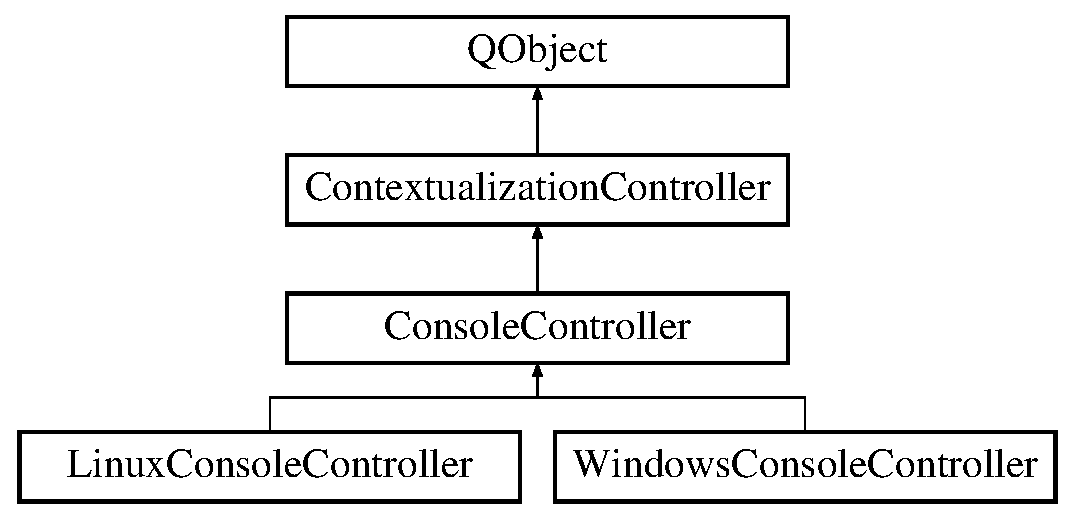
\includegraphics[height=4.000000cm]{classConsoleController}
\end{center}
\end{figure}
\subsection*{Public Types}
\begin{DoxyCompactItemize}
\item 
enum \mbox{\hyperlink{classConsoleController_a6bc36e6ee00aa2da0fd9be549b4251d9}{Action\+Type}} \{ \newline
\mbox{\hyperlink{classConsoleController_a6bc36e6ee00aa2da0fd9be549b4251d9a0fada6cf25abb68366ac353a6ec646e0}{Print\+Help}} = 0, 
\mbox{\hyperlink{classConsoleController_a6bc36e6ee00aa2da0fd9be549b4251d9ab376541b60038f69f8575f6fe680f9d2}{No\+Action}}, 
\mbox{\hyperlink{classConsoleController_a6bc36e6ee00aa2da0fd9be549b4251d9a04bb2e774b79ceb4bc2979c400e8feea}{List\+Projects}}, 
\mbox{\hyperlink{classConsoleController_a6bc36e6ee00aa2da0fd9be549b4251d9a230f00a5b6250550356eb456475fe757}{Detail\+Project}}, 
\newline
\mbox{\hyperlink{classConsoleController_a6bc36e6ee00aa2da0fd9be549b4251d9a9963a057c42713ecf9380500367f621b}{New\+Project}}, 
\mbox{\hyperlink{classConsoleController_a6bc36e6ee00aa2da0fd9be549b4251d9aa620b51a7f0e47c93da8f023ca37a81b}{Delete\+Project}}, 
\mbox{\hyperlink{classConsoleController_a6bc36e6ee00aa2da0fd9be549b4251d9a39ac9ee6f36481423172c8c7957beb50}{Select\+Project}}, 
\mbox{\hyperlink{classConsoleController_a6bc36e6ee00aa2da0fd9be549b4251d9a784b89a27e92a50096f0af414cc7f4ad}{Clear\+Strings}}, 
\newline
\mbox{\hyperlink{classConsoleController_a6bc36e6ee00aa2da0fd9be549b4251d9a4d8a085e65fdc727d7642a25db2403b2}{Clear\+Image}}, 
\mbox{\hyperlink{classConsoleController_a6bc36e6ee00aa2da0fd9be549b4251d9adc51bd8437c400c4193fa01650c087a0}{Clear\+All}}, 
\mbox{\hyperlink{classConsoleController_a6bc36e6ee00aa2da0fd9be549b4251d9a121c3067d3adf19104793ce9020fb543}{Add\+String}}, 
\mbox{\hyperlink{classConsoleController_a6bc36e6ee00aa2da0fd9be549b4251d9adf314576f39f9dfe3ce14758e7482422}{Remove\+String}}, 
\newline
\mbox{\hyperlink{classConsoleController_a6bc36e6ee00aa2da0fd9be549b4251d9abe2b103c6a30c1a23b13772970452b03}{Select\+String}}, 
\mbox{\hyperlink{classConsoleController_a6bc36e6ee00aa2da0fd9be549b4251d9acedfdd10ac8c789aa7d4dd9f78bd3937}{Unselect\+String}}, 
\mbox{\hyperlink{classConsoleController_a6bc36e6ee00aa2da0fd9be549b4251d9a346b6628a5522d04a57e23fd96b14e94}{Set\+Image}}, 
\mbox{\hyperlink{classConsoleController_a6bc36e6ee00aa2da0fd9be549b4251d9ac281d38e622624b8d89974cd1a437243}{Capture\+Area}}, 
\newline
\mbox{\hyperlink{classConsoleController_a6bc36e6ee00aa2da0fd9be549b4251d9af2fd8b4a218c3ddbc0fd91c5b1667693}{Detect\+Strings}}, 
\mbox{\hyperlink{classConsoleController_a6bc36e6ee00aa2da0fd9be549b4251d9ab2dae62af54e26573bd66ca8f9ee3f0a}{Export\+Project}}, 
\mbox{\hyperlink{classConsoleController_a6bc36e6ee00aa2da0fd9be549b4251d9aa66215a16eaf6c015d2569d4574572a9}{Import\+Project}}, 
\mbox{\hyperlink{classConsoleController_a6bc36e6ee00aa2da0fd9be549b4251d9a20e0cfce6c39df1ac1c1552ddf2dde22}{Send}}, 
\newline
\mbox{\hyperlink{classConsoleController_a6bc36e6ee00aa2da0fd9be549b4251d9a465c31f22f889f262d21e867223c19a9}{Process\+Files}}, 
\mbox{\hyperlink{classConsoleController_a6bc36e6ee00aa2da0fd9be549b4251d9a019ca0fceccfad49f6abea9cee533222}{Print\+Clear\+Help}}, 
\mbox{\hyperlink{classConsoleController_a6bc36e6ee00aa2da0fd9be549b4251d9ad1953c9265bcc1cb3663f2ccc23c5810}{Print\+Add\+Help}}, 
\mbox{\hyperlink{classConsoleController_a6bc36e6ee00aa2da0fd9be549b4251d9a1a9ee810a12e81b7cbcb5f74a59e1b76}{Print\+Detect\+Help}}, 
\newline
\mbox{\hyperlink{classConsoleController_a6bc36e6ee00aa2da0fd9be549b4251d9a2cc22e62323a75b556c4e7568f9e588f}{Print\+Image\+Help}}
 \}
\begin{DoxyCompactList}\small\item\em Constains all actions that can be done by the exec function. \end{DoxyCompactList}\end{DoxyCompactItemize}
\subsection*{Public Member Functions}
\begin{DoxyCompactItemize}
\item 
\mbox{\Hypertarget{classConsoleController_aed7f998b076f322a0c45f0a0e57202c4}\label{classConsoleController_aed7f998b076f322a0c45f0a0e57202c4}} 
\mbox{\hyperlink{classConsoleController_aed7f998b076f322a0c45f0a0e57202c4}{Console\+Controller}} ()
\begin{DoxyCompactList}\small\item\em Creates an empty controller. \end{DoxyCompactList}\item 
\mbox{\hyperlink{classConsoleController_aaf8a775d3f675bcf9e7facd959217fdc}{Console\+Controller}} (int argc, char $\ast$$\ast$argv)
\begin{DoxyCompactList}\small\item\em Creates a controller decoding arguments received by argument. \end{DoxyCompactList}\item 
void \mbox{\hyperlink{classConsoleController_accdfd546eef82cfe4d0942426a3b6fac}{exec}} ()
\begin{DoxyCompactList}\small\item\em Executes the logic of controller. \end{DoxyCompactList}\item 
bool \mbox{\hyperlink{classConsoleController_ab9fdcba75eecb1f28c1fcd3b97183fe8}{decode\+Arguments}} (int argc, char $\ast$$\ast$argv)
\begin{DoxyCompactList}\small\item\em Decode arguments entered to set the behavior of the exec method. \end{DoxyCompactList}\item 
void \mbox{\hyperlink{classConsoleController_a13eaf91bd8d72afeaa3792255983e019}{set\+Action}} (\mbox{\hyperlink{classConsoleController_a6bc36e6ee00aa2da0fd9be549b4251d9}{Action\+Type}} action, Q\+Variant parameter=Q\+Variant())
\begin{DoxyCompactList}\small\item\em Sets the action to be executed and his parameter,. \end{DoxyCompactList}\item 
\mbox{\Hypertarget{classConsoleController_a771c221ac40cd6441f13c76bd08b6927}\label{classConsoleController_a771c221ac40cd6441f13c76bd08b6927}} 
void \mbox{\hyperlink{classConsoleController_a771c221ac40cd6441f13c76bd08b6927}{print\+Usage}} ()
\begin{DoxyCompactList}\small\item\em Print in screen the general usage of application. \end{DoxyCompactList}\item 
\mbox{\Hypertarget{classConsoleController_a08cea6c7cb62ea9961af568daeec69c5}\label{classConsoleController_a08cea6c7cb62ea9961af568daeec69c5}} 
void \mbox{\hyperlink{classConsoleController_a08cea6c7cb62ea9961af568daeec69c5}{print\+Clear\+Details}} ()
\begin{DoxyCompactList}\small\item\em Print extended help for clear command. \end{DoxyCompactList}\item 
\mbox{\Hypertarget{classConsoleController_a5e2c72a9589fc8b5a2d9ba5c905850c8}\label{classConsoleController_a5e2c72a9589fc8b5a2d9ba5c905850c8}} 
void \mbox{\hyperlink{classConsoleController_a5e2c72a9589fc8b5a2d9ba5c905850c8}{print\+Add\+Details}} ()
\begin{DoxyCompactList}\small\item\em Print extended help for add command. \end{DoxyCompactList}\item 
\mbox{\Hypertarget{classConsoleController_aeef4c9eb3a199d0674c0841eadad6d7e}\label{classConsoleController_aeef4c9eb3a199d0674c0841eadad6d7e}} 
void \mbox{\hyperlink{classConsoleController_aeef4c9eb3a199d0674c0841eadad6d7e}{print\+Detect\+Details}} ()
\begin{DoxyCompactList}\small\item\em Print extended help for detect command. \end{DoxyCompactList}\item 
\mbox{\Hypertarget{classConsoleController_ae99f394b6610fd7c771e31d864526756}\label{classConsoleController_ae99f394b6610fd7c771e31d864526756}} 
void \mbox{\hyperlink{classConsoleController_ae99f394b6610fd7c771e31d864526756}{print\+Image\+Details}} ()
\begin{DoxyCompactList}\small\item\em Print extended help for image command. \end{DoxyCompactList}\item 
\mbox{\Hypertarget{classConsoleController_a5dd7913a42068df42c3de6dc1f313537}\label{classConsoleController_a5dd7913a42068df42c3de6dc1f313537}} 
void \mbox{\hyperlink{classConsoleController_a5dd7913a42068df42c3de6dc1f313537}{print\+Detect\+Options}} ()
\begin{DoxyCompactList}\small\item\em Print extended help for detect command. \end{DoxyCompactList}\end{DoxyCompactItemize}
\subsection*{Additional Inherited Members}


\subsection{Detailed Description}
The Console\+Contextualization\+Controller class is responsible for controll the Contextualization Tool application when is executed from a terminal (C\+LI). 

This is the controller class that works a C\+LI environment. 

Definition at line 26 of file consolecontroller.\+h.



\subsection{Member Enumeration Documentation}
\mbox{\Hypertarget{classConsoleController_a6bc36e6ee00aa2da0fd9be549b4251d9}\label{classConsoleController_a6bc36e6ee00aa2da0fd9be549b4251d9}} 
\index{Console\+Controller@{Console\+Controller}!Action\+Type@{Action\+Type}}
\index{Action\+Type@{Action\+Type}!Console\+Controller@{Console\+Controller}}
\subsubsection{\texorpdfstring{Action\+Type}{ActionType}}
{\footnotesize\ttfamily enum \mbox{\hyperlink{classConsoleController_a6bc36e6ee00aa2da0fd9be549b4251d9}{Console\+Controller\+::\+Action\+Type}}}



Constains all actions that can be done by the exec function. 

\begin{DoxyEnumFields}{Enumerator}
\raisebox{\heightof{T}}[0pt][0pt]{\index{Print\+Help@{Print\+Help}!Console\+Controller@{Console\+Controller}}\index{Console\+Controller@{Console\+Controller}!Print\+Help@{Print\+Help}}}\mbox{\Hypertarget{classConsoleController_a6bc36e6ee00aa2da0fd9be549b4251d9a0fada6cf25abb68366ac353a6ec646e0}\label{classConsoleController_a6bc36e6ee00aa2da0fd9be549b4251d9a0fada6cf25abb68366ac353a6ec646e0}} 
Print\+Help&Indicates that the app have to print the general help. \\
\hline

\raisebox{\heightof{T}}[0pt][0pt]{\index{No\+Action@{No\+Action}!Console\+Controller@{Console\+Controller}}\index{Console\+Controller@{Console\+Controller}!No\+Action@{No\+Action}}}\mbox{\Hypertarget{classConsoleController_a6bc36e6ee00aa2da0fd9be549b4251d9ab376541b60038f69f8575f6fe680f9d2}\label{classConsoleController_a6bc36e6ee00aa2da0fd9be549b4251d9ab376541b60038f69f8575f6fe680f9d2}} 
No\+Action&Indicates that the app have to do anything. \\
\hline

\raisebox{\heightof{T}}[0pt][0pt]{\index{List\+Projects@{List\+Projects}!Console\+Controller@{Console\+Controller}}\index{Console\+Controller@{Console\+Controller}!List\+Projects@{List\+Projects}}}\mbox{\Hypertarget{classConsoleController_a6bc36e6ee00aa2da0fd9be549b4251d9a04bb2e774b79ceb4bc2979c400e8feea}\label{classConsoleController_a6bc36e6ee00aa2da0fd9be549b4251d9a04bb2e774b79ceb4bc2979c400e8feea}} 
List\+Projects&Indicates that the app have to list all available projects. \\
\hline

\raisebox{\heightof{T}}[0pt][0pt]{\index{Detail\+Project@{Detail\+Project}!Console\+Controller@{Console\+Controller}}\index{Console\+Controller@{Console\+Controller}!Detail\+Project@{Detail\+Project}}}\mbox{\Hypertarget{classConsoleController_a6bc36e6ee00aa2da0fd9be549b4251d9a230f00a5b6250550356eb456475fe757}\label{classConsoleController_a6bc36e6ee00aa2da0fd9be549b4251d9a230f00a5b6250550356eb456475fe757}} 
Detail\+Project&Indicates that the app have to show detail for avitve project. \\
\hline

\raisebox{\heightof{T}}[0pt][0pt]{\index{New\+Project@{New\+Project}!Console\+Controller@{Console\+Controller}}\index{Console\+Controller@{Console\+Controller}!New\+Project@{New\+Project}}}\mbox{\Hypertarget{classConsoleController_a6bc36e6ee00aa2da0fd9be549b4251d9a9963a057c42713ecf9380500367f621b}\label{classConsoleController_a6bc36e6ee00aa2da0fd9be549b4251d9a9963a057c42713ecf9380500367f621b}} 
New\+Project&Indicates that the app have to create new project. \\
\hline

\raisebox{\heightof{T}}[0pt][0pt]{\index{Delete\+Project@{Delete\+Project}!Console\+Controller@{Console\+Controller}}\index{Console\+Controller@{Console\+Controller}!Delete\+Project@{Delete\+Project}}}\mbox{\Hypertarget{classConsoleController_a6bc36e6ee00aa2da0fd9be549b4251d9aa620b51a7f0e47c93da8f023ca37a81b}\label{classConsoleController_a6bc36e6ee00aa2da0fd9be549b4251d9aa620b51a7f0e47c93da8f023ca37a81b}} 
Delete\+Project&Indicates that the app have to delete a project. \\
\hline

\raisebox{\heightof{T}}[0pt][0pt]{\index{Select\+Project@{Select\+Project}!Console\+Controller@{Console\+Controller}}\index{Console\+Controller@{Console\+Controller}!Select\+Project@{Select\+Project}}}\mbox{\Hypertarget{classConsoleController_a6bc36e6ee00aa2da0fd9be549b4251d9a39ac9ee6f36481423172c8c7957beb50}\label{classConsoleController_a6bc36e6ee00aa2da0fd9be549b4251d9a39ac9ee6f36481423172c8c7957beb50}} 
Select\+Project&Indicates that the app have to ativate a project. \\
\hline

\raisebox{\heightof{T}}[0pt][0pt]{\index{Clear\+Strings@{Clear\+Strings}!Console\+Controller@{Console\+Controller}}\index{Console\+Controller@{Console\+Controller}!Clear\+Strings@{Clear\+Strings}}}\mbox{\Hypertarget{classConsoleController_a6bc36e6ee00aa2da0fd9be549b4251d9a784b89a27e92a50096f0af414cc7f4ad}\label{classConsoleController_a6bc36e6ee00aa2da0fd9be549b4251d9a784b89a27e92a50096f0af414cc7f4ad}} 
Clear\+Strings&Indicates that the app have to clear all strings from the active project. \\
\hline

\raisebox{\heightof{T}}[0pt][0pt]{\index{Clear\+Image@{Clear\+Image}!Console\+Controller@{Console\+Controller}}\index{Console\+Controller@{Console\+Controller}!Clear\+Image@{Clear\+Image}}}\mbox{\Hypertarget{classConsoleController_a6bc36e6ee00aa2da0fd9be549b4251d9a4d8a085e65fdc727d7642a25db2403b2}\label{classConsoleController_a6bc36e6ee00aa2da0fd9be549b4251d9a4d8a085e65fdc727d7642a25db2403b2}} 
Clear\+Image&Indicates that the app have to unset current image from the active project. \\
\hline

\raisebox{\heightof{T}}[0pt][0pt]{\index{Clear\+All@{Clear\+All}!Console\+Controller@{Console\+Controller}}\index{Console\+Controller@{Console\+Controller}!Clear\+All@{Clear\+All}}}\mbox{\Hypertarget{classConsoleController_a6bc36e6ee00aa2da0fd9be549b4251d9adc51bd8437c400c4193fa01650c087a0}\label{classConsoleController_a6bc36e6ee00aa2da0fd9be549b4251d9adc51bd8437c400c4193fa01650c087a0}} 
Clear\+All&Indicates that the app have to empty the active project. \\
\hline

\raisebox{\heightof{T}}[0pt][0pt]{\index{Add\+String@{Add\+String}!Console\+Controller@{Console\+Controller}}\index{Console\+Controller@{Console\+Controller}!Add\+String@{Add\+String}}}\mbox{\Hypertarget{classConsoleController_a6bc36e6ee00aa2da0fd9be549b4251d9a121c3067d3adf19104793ce9020fb543}\label{classConsoleController_a6bc36e6ee00aa2da0fd9be549b4251d9a121c3067d3adf19104793ce9020fb543}} 
Add\+String&Indicates that the app have to add new string in the active project. \\
\hline

\raisebox{\heightof{T}}[0pt][0pt]{\index{Remove\+String@{Remove\+String}!Console\+Controller@{Console\+Controller}}\index{Console\+Controller@{Console\+Controller}!Remove\+String@{Remove\+String}}}\mbox{\Hypertarget{classConsoleController_a6bc36e6ee00aa2da0fd9be549b4251d9adf314576f39f9dfe3ce14758e7482422}\label{classConsoleController_a6bc36e6ee00aa2da0fd9be549b4251d9adf314576f39f9dfe3ce14758e7482422}} 
Remove\+String&Indicates that the app have to remove a string from the active project. \\
\hline

\raisebox{\heightof{T}}[0pt][0pt]{\index{Select\+String@{Select\+String}!Console\+Controller@{Console\+Controller}}\index{Console\+Controller@{Console\+Controller}!Select\+String@{Select\+String}}}\mbox{\Hypertarget{classConsoleController_a6bc36e6ee00aa2da0fd9be549b4251d9abe2b103c6a30c1a23b13772970452b03}\label{classConsoleController_a6bc36e6ee00aa2da0fd9be549b4251d9abe2b103c6a30c1a23b13772970452b03}} 
Select\+String&Indicates that the app have to select the string indicated by user. \\
\hline

\raisebox{\heightof{T}}[0pt][0pt]{\index{Unselect\+String@{Unselect\+String}!Console\+Controller@{Console\+Controller}}\index{Console\+Controller@{Console\+Controller}!Unselect\+String@{Unselect\+String}}}\mbox{\Hypertarget{classConsoleController_a6bc36e6ee00aa2da0fd9be549b4251d9acedfdd10ac8c789aa7d4dd9f78bd3937}\label{classConsoleController_a6bc36e6ee00aa2da0fd9be549b4251d9acedfdd10ac8c789aa7d4dd9f78bd3937}} 
Unselect\+String&Indicates that the app have to unselect the string indicated by user. \\
\hline

\raisebox{\heightof{T}}[0pt][0pt]{\index{Set\+Image@{Set\+Image}!Console\+Controller@{Console\+Controller}}\index{Console\+Controller@{Console\+Controller}!Set\+Image@{Set\+Image}}}\mbox{\Hypertarget{classConsoleController_a6bc36e6ee00aa2da0fd9be549b4251d9a346b6628a5522d04a57e23fd96b14e94}\label{classConsoleController_a6bc36e6ee00aa2da0fd9be549b4251d9a346b6628a5522d04a57e23fd96b14e94}} 
Set\+Image&Indicates that the app have to set the image in the active project. \\
\hline

\raisebox{\heightof{T}}[0pt][0pt]{\index{Capture\+Area@{Capture\+Area}!Console\+Controller@{Console\+Controller}}\index{Console\+Controller@{Console\+Controller}!Capture\+Area@{Capture\+Area}}}\mbox{\Hypertarget{classConsoleController_a6bc36e6ee00aa2da0fd9be549b4251d9ac281d38e622624b8d89974cd1a437243}\label{classConsoleController_a6bc36e6ee00aa2da0fd9be549b4251d9ac281d38e622624b8d89974cd1a437243}} 
Capture\+Area&Indicates that the app have to let the user capture an area of sreen and set it as image model. \\
\hline

\raisebox{\heightof{T}}[0pt][0pt]{\index{Detect\+Strings@{Detect\+Strings}!Console\+Controller@{Console\+Controller}}\index{Console\+Controller@{Console\+Controller}!Detect\+Strings@{Detect\+Strings}}}\mbox{\Hypertarget{classConsoleController_a6bc36e6ee00aa2da0fd9be549b4251d9af2fd8b4a218c3ddbc0fd91c5b1667693}\label{classConsoleController_a6bc36e6ee00aa2da0fd9be549b4251d9af2fd8b4a218c3ddbc0fd91c5b1667693}} 
Detect\+Strings&Indicates that the app have to extract strings from image model and add it in active project. \\
\hline

\raisebox{\heightof{T}}[0pt][0pt]{\index{Export\+Project@{Export\+Project}!Console\+Controller@{Console\+Controller}}\index{Console\+Controller@{Console\+Controller}!Export\+Project@{Export\+Project}}}\mbox{\Hypertarget{classConsoleController_a6bc36e6ee00aa2da0fd9be549b4251d9ab2dae62af54e26573bd66ca8f9ee3f0a}\label{classConsoleController_a6bc36e6ee00aa2da0fd9be549b4251d9ab2dae62af54e26573bd66ca8f9ee3f0a}} 
Export\+Project&Indicates that the app have to save the active project in the path entered by the user. \\
\hline

\raisebox{\heightof{T}}[0pt][0pt]{\index{Import\+Project@{Import\+Project}!Console\+Controller@{Console\+Controller}}\index{Console\+Controller@{Console\+Controller}!Import\+Project@{Import\+Project}}}\mbox{\Hypertarget{classConsoleController_a6bc36e6ee00aa2da0fd9be549b4251d9aa66215a16eaf6c015d2569d4574572a9}\label{classConsoleController_a6bc36e6ee00aa2da0fd9be549b4251d9aa66215a16eaf6c015d2569d4574572a9}} 
Import\+Project&Indicates that the app have to import a project entered by the user. \\
\hline

\raisebox{\heightof{T}}[0pt][0pt]{\index{Send@{Send}!Console\+Controller@{Console\+Controller}}\index{Console\+Controller@{Console\+Controller}!Send@{Send}}}\mbox{\Hypertarget{classConsoleController_a6bc36e6ee00aa2da0fd9be549b4251d9a20e0cfce6c39df1ac1c1552ddf2dde22}\label{classConsoleController_a6bc36e6ee00aa2da0fd9be549b4251d9a20e0cfce6c39df1ac1c1552ddf2dde22}} 
Send&Indicates that the app have to send the active contextualization. \\
\hline

\raisebox{\heightof{T}}[0pt][0pt]{\index{Process\+Files@{Process\+Files}!Console\+Controller@{Console\+Controller}}\index{Console\+Controller@{Console\+Controller}!Process\+Files@{Process\+Files}}}\mbox{\Hypertarget{classConsoleController_a6bc36e6ee00aa2da0fd9be549b4251d9a465c31f22f889f262d21e867223c19a9}\label{classConsoleController_a6bc36e6ee00aa2da0fd9be549b4251d9a465c31f22f889f262d21e867223c19a9}} 
Process\+Files&Indicates that the app have to process files and storage V\+A\+L\+I\+D\+A\+D\+ED strings. \\
\hline

\raisebox{\heightof{T}}[0pt][0pt]{\index{Print\+Clear\+Help@{Print\+Clear\+Help}!Console\+Controller@{Console\+Controller}}\index{Console\+Controller@{Console\+Controller}!Print\+Clear\+Help@{Print\+Clear\+Help}}}\mbox{\Hypertarget{classConsoleController_a6bc36e6ee00aa2da0fd9be549b4251d9a019ca0fceccfad49f6abea9cee533222}\label{classConsoleController_a6bc36e6ee00aa2da0fd9be549b4251d9a019ca0fceccfad49f6abea9cee533222}} 
Print\+Clear\+Help&Indicates that the app have to print detailed help for clear command. \\
\hline

\raisebox{\heightof{T}}[0pt][0pt]{\index{Print\+Add\+Help@{Print\+Add\+Help}!Console\+Controller@{Console\+Controller}}\index{Console\+Controller@{Console\+Controller}!Print\+Add\+Help@{Print\+Add\+Help}}}\mbox{\Hypertarget{classConsoleController_a6bc36e6ee00aa2da0fd9be549b4251d9ad1953c9265bcc1cb3663f2ccc23c5810}\label{classConsoleController_a6bc36e6ee00aa2da0fd9be549b4251d9ad1953c9265bcc1cb3663f2ccc23c5810}} 
Print\+Add\+Help&Indicates that the app have to print extended help for add command. \\
\hline

\raisebox{\heightof{T}}[0pt][0pt]{\index{Print\+Detect\+Help@{Print\+Detect\+Help}!Console\+Controller@{Console\+Controller}}\index{Console\+Controller@{Console\+Controller}!Print\+Detect\+Help@{Print\+Detect\+Help}}}\mbox{\Hypertarget{classConsoleController_a6bc36e6ee00aa2da0fd9be549b4251d9a1a9ee810a12e81b7cbcb5f74a59e1b76}\label{classConsoleController_a6bc36e6ee00aa2da0fd9be549b4251d9a1a9ee810a12e81b7cbcb5f74a59e1b76}} 
Print\+Detect\+Help&Indicates that the app have to print extended help for detect command. \\
\hline

\raisebox{\heightof{T}}[0pt][0pt]{\index{Print\+Image\+Help@{Print\+Image\+Help}!Console\+Controller@{Console\+Controller}}\index{Console\+Controller@{Console\+Controller}!Print\+Image\+Help@{Print\+Image\+Help}}}\mbox{\Hypertarget{classConsoleController_a6bc36e6ee00aa2da0fd9be549b4251d9a2cc22e62323a75b556c4e7568f9e588f}\label{classConsoleController_a6bc36e6ee00aa2da0fd9be549b4251d9a2cc22e62323a75b556c4e7568f9e588f}} 
Print\+Image\+Help&Indicates that the app have to print extended help for image command. \\
\hline

\end{DoxyEnumFields}


Definition at line 33 of file consolecontroller.\+h.



\subsection{Constructor \& Destructor Documentation}
\mbox{\Hypertarget{classConsoleController_aaf8a775d3f675bcf9e7facd959217fdc}\label{classConsoleController_aaf8a775d3f675bcf9e7facd959217fdc}} 
\index{Console\+Controller@{Console\+Controller}!Console\+Controller@{Console\+Controller}}
\index{Console\+Controller@{Console\+Controller}!Console\+Controller@{Console\+Controller}}
\subsubsection{\texorpdfstring{Console\+Controller()}{ConsoleController()}}
{\footnotesize\ttfamily Console\+Controller\+::\+Console\+Controller (\begin{DoxyParamCaption}\item[{int}]{argc,  }\item[{char $\ast$$\ast$}]{argv }\end{DoxyParamCaption})}



Creates a controller decoding arguments received by argument. 


\begin{DoxyParams}{Parameters}
{\em argc} & Number of argv elements. \\
\hline
{\em argv} & Arguments entered by the user when executed the app. \\
\hline
\end{DoxyParams}


Definition at line 22 of file consolecontroller.\+cpp.



\subsection{Member Function Documentation}
\mbox{\Hypertarget{classConsoleController_ab9fdcba75eecb1f28c1fcd3b97183fe8}\label{classConsoleController_ab9fdcba75eecb1f28c1fcd3b97183fe8}} 
\index{Console\+Controller@{Console\+Controller}!decode\+Arguments@{decode\+Arguments}}
\index{decode\+Arguments@{decode\+Arguments}!Console\+Controller@{Console\+Controller}}
\subsubsection{\texorpdfstring{decode\+Arguments()}{decodeArguments()}}
{\footnotesize\ttfamily bool Console\+Controller\+::decode\+Arguments (\begin{DoxyParamCaption}\item[{int}]{argc,  }\item[{char $\ast$$\ast$}]{argv }\end{DoxyParamCaption})}



Decode arguments entered to set the behavior of the exec method. 

The first element of argv always must be the name of the app. 
\begin{DoxyParams}{Parameters}
{\em argc} & Number of argv elements. \\
\hline
{\em argv} & Arguments to decode. \\
\hline
\end{DoxyParams}
\begin{DoxyReturn}{Returns}

\end{DoxyReturn}


Definition at line 120 of file consolecontroller.\+cpp.

\mbox{\Hypertarget{classConsoleController_accdfd546eef82cfe4d0942426a3b6fac}\label{classConsoleController_accdfd546eef82cfe4d0942426a3b6fac}} 
\index{Console\+Controller@{Console\+Controller}!exec@{exec}}
\index{exec@{exec}!Console\+Controller@{Console\+Controller}}
\subsubsection{\texorpdfstring{exec()}{exec()}}
{\footnotesize\ttfamily void Console\+Controller\+::exec (\begin{DoxyParamCaption}{ }\end{DoxyParamCaption})}



Executes the logic of controller. 

It has mutiples type of behavior depending the value of action\+\_\+ variable.

Types of action can be shown in Action\+Type enum. 

Definition at line 36 of file consolecontroller.\+cpp.

\mbox{\Hypertarget{classConsoleController_a13eaf91bd8d72afeaa3792255983e019}\label{classConsoleController_a13eaf91bd8d72afeaa3792255983e019}} 
\index{Console\+Controller@{Console\+Controller}!set\+Action@{set\+Action}}
\index{set\+Action@{set\+Action}!Console\+Controller@{Console\+Controller}}
\subsubsection{\texorpdfstring{set\+Action()}{setAction()}}
{\footnotesize\ttfamily void Console\+Controller\+::set\+Action (\begin{DoxyParamCaption}\item[{\mbox{\hyperlink{classConsoleController_a6bc36e6ee00aa2da0fd9be549b4251d9}{Action\+Type}}}]{action,  }\item[{Q\+Variant}]{parameter = {\ttfamily QVariant()} }\end{DoxyParamCaption})\hspace{0.3cm}{\ttfamily [inline]}}



Sets the action to be executed and his parameter,. 


\begin{DoxyParams}{Parameters}
{\em action} & Actions to be executed by \mbox{\hyperlink{classConsoleController_accdfd546eef82cfe4d0942426a3b6fac}{exec()}} function. \\
\hline
{\em parameter} & Required parameter to execute the action. \\
\hline
\end{DoxyParams}


Definition at line 244 of file consolecontroller.\+cpp.



The documentation for this class was generated from the following files\+:\begin{DoxyCompactItemize}
\item 
src/contextualization/controller/\mbox{\hyperlink{consolecontroller_8h}{consolecontroller.\+h}}\item 
src/contextualization/controller/\mbox{\hyperlink{consolecontroller_8cpp}{consolecontroller.\+cpp}}\end{DoxyCompactItemize}

\hypertarget{classContextualizationController}{}\section{Contextualization\+Controller Class Reference}
\label{classContextualizationController}\index{Contextualization\+Controller@{Contextualization\+Controller}}


This is the controller base class.  




{\ttfamily \#include $<$contextualizationcontroller.\+h$>$}

Inheritance diagram for Contextualization\+Controller\+:\begin{figure}[H]
\begin{center}
\leavevmode
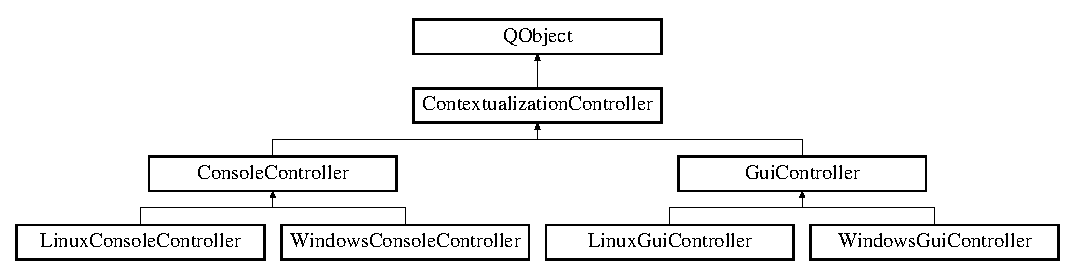
\includegraphics[height=3.255814cm]{classContextualizationController}
\end{center}
\end{figure}
\subsection*{Public Types}
\begin{DoxyCompactItemize}
\item 
enum \mbox{\hyperlink{classContextualizationController_a78e15dc8f6f1e0cb4df6d86b921be8a4}{Model\+Error}} \{ \mbox{\hyperlink{classContextualizationController_a78e15dc8f6f1e0cb4df6d86b921be8a4a6ccff3cdedbdcfcdfc1eb59c4b088d24}{Ok\+Model}} = 0, 
\mbox{\hyperlink{classContextualizationController_a78e15dc8f6f1e0cb4df6d86b921be8a4adba539af7fd279d01da3a2a1e91e40ca}{No\+Image}}, 
\mbox{\hyperlink{classContextualizationController_a78e15dc8f6f1e0cb4df6d86b921be8a4a5d1b78a6b1296da8bf43b62432d090c5}{Image\+Not\+Exist}}, 
\mbox{\hyperlink{classContextualizationController_a78e15dc8f6f1e0cb4df6d86b921be8a4a2e771e637c2e37c6b410a96c9f48adfd}{No\+Strings}}
 \}
\begin{DoxyCompactList}\small\item\em The Model\+Error enum. \end{DoxyCompactList}\item 
enum \mbox{\hyperlink{classContextualizationController_acb38587f7f9e610a5950956b345d69fd}{Code\+Error}} \{ \newline
\mbox{\hyperlink{classContextualizationController_acb38587f7f9e610a5950956b345d69fdac799a856f8460c5e6b100f08191b2d94}{No\+Error}} = 0, 
\mbox{\hyperlink{classContextualizationController_acb38587f7f9e610a5950956b345d69fda067a46ac62df6062561a10108b8e77a9}{Null\+Pointer}}, 
\mbox{\hyperlink{classContextualizationController_acb38587f7f9e610a5950956b345d69fda4a6ad284235290da632cd7b621ae53be}{String\+Already\+Exists}}, 
\mbox{\hyperlink{classContextualizationController_acb38587f7f9e610a5950956b345d69fdac9ac40727cb32c37655f627ecd1450d4}{No\+Import\+File}}, 
\newline
\mbox{\hyperlink{classContextualizationController_acb38587f7f9e610a5950956b345d69fda705a292a89a7c137ed934a1ede90968a}{Import\+File\+Format}}, 
\mbox{\hyperlink{classContextualizationController_acb38587f7f9e610a5950956b345d69fdad866e236894ecf819409ebb4d44b7fd1}{File\+Not\+Exists}}, 
\mbox{\hyperlink{classContextualizationController_acb38587f7f9e610a5950956b345d69fda3da219148b52a6691d2dbcd9f40ed627}{No\+Remote\+Host}}, 
\mbox{\hyperlink{classContextualizationController_acb38587f7f9e610a5950956b345d69fda5360679b825af2b3b97283fae1a9717a}{No\+Valid\+Ip}}, 
\newline
\mbox{\hyperlink{classContextualizationController_acb38587f7f9e610a5950956b345d69fda860490b2223e4e78d29a514fb51f6fc5}{Sshpass\+Error}} = 254, 
\mbox{\hyperlink{classContextualizationController_acb38587f7f9e610a5950956b345d69fda7447fb0b9cf45b0adc6da65c65c34253}{Ssh\+Error}} = 255, 
\mbox{\hyperlink{classContextualizationController_acb38587f7f9e610a5950956b345d69fda841e3c0b31b4da700505de6d3b30dabe}{Write\+File}} = -\/1
 \}
\begin{DoxyCompactList}\small\item\em The Code\+Error enum. \end{DoxyCompactList}\item 
enum \mbox{\hyperlink{classContextualizationController_a211b7dd2dba820139e8055b4f88fdced}{Match\+Type}} \{ \mbox{\hyperlink{classContextualizationController_a211b7dd2dba820139e8055b4f88fdcedab921b1883492c5a7511b20ec6a5f24f3}{By\+ID}} = 0, 
\mbox{\hyperlink{classContextualizationController_a211b7dd2dba820139e8055b4f88fdceda0e89844c93d199f9e314fc1a1ddae400}{By\+Value}}, 
\mbox{\hyperlink{classContextualizationController_a211b7dd2dba820139e8055b4f88fdceda54d0f26a3c6d7f680f2bcbd383f1d9df}{By\+Approximate\+Value}}
 \}
\begin{DoxyCompactList}\small\item\em The Match\+Type enum. \end{DoxyCompactList}\end{DoxyCompactItemize}
\subsection*{Signals}
\begin{DoxyCompactItemize}
\item 
\mbox{\Hypertarget{classContextualizationController_a0040eddc367f6685480818a2fd9d7a25}\label{classContextualizationController_a0040eddc367f6685480818a2fd9d7a25}} 
void \mbox{\hyperlink{classContextualizationController_a0040eddc367f6685480818a2fd9d7a25}{strings\+List\+Changed}} ()
\begin{DoxyCompactList}\small\item\em The signal is emitted when a new string is added to the model or a string is removed from the model. \end{DoxyCompactList}\item 
\mbox{\Hypertarget{classContextualizationController_ac101eb9c6edbc62b829257c4cfcc9fe1}\label{classContextualizationController_ac101eb9c6edbc62b829257c4cfcc9fe1}} 
void \mbox{\hyperlink{classContextualizationController_ac101eb9c6edbc62b829257c4cfcc9fe1}{image\+Changed}} ()
\begin{DoxyCompactList}\small\item\em The signal is emitted when a image is setted on the model. \end{DoxyCompactList}\end{DoxyCompactItemize}
\subsection*{Public Member Functions}
\begin{DoxyCompactItemize}
\item 
\mbox{\hyperlink{classContextualizationController_a055cc7f78056ccc0d0a55023402a29ee}{Contextualization\+Controller}} (Q\+Object $\ast$parent=Q\+\_\+\+N\+U\+L\+L\+P\+TR)
\begin{DoxyCompactList}\small\item\em Constructs a controller setting his member variables. \end{DoxyCompactList}\item 
\mbox{\Hypertarget{classContextualizationController_ae5b1fa3bf3a7b92c8454e8cd98558989}\label{classContextualizationController_ae5b1fa3bf3a7b92c8454e8cd98558989}} 
\mbox{\hyperlink{classContextualizationController_ae5b1fa3bf3a7b92c8454e8cd98558989}{$\sim$\+Contextualization\+Controller}} ()
\begin{DoxyCompactList}\small\item\em Destroys the controller. \end{DoxyCompactList}\end{DoxyCompactItemize}
\subsection*{Protected Slots}
\begin{DoxyCompactItemize}
\item 
virtual void \mbox{\hyperlink{classContextualizationController_afea4c16fa2728506e6301e46891bf73f}{add}} (Q\+String new\+String, int match\+Type)=0
\begin{DoxyCompactList}\small\item\em Tries to add a new string into the model. \end{DoxyCompactList}\item 
virtual void \mbox{\hyperlink{classContextualizationController_ae06d4c794e77321439668aadc141aca5}{remove}} (Q\+String string\+Id)=0
\begin{DoxyCompactList}\small\item\em Tries to remove the string in the model with the identifier receiven by parameter. \end{DoxyCompactList}\item 
\mbox{\Hypertarget{classContextualizationController_a2f19977180ae0d6ecd3900951d686fe3}\label{classContextualizationController_a2f19977180ae0d6ecd3900951d686fe3}} 
virtual void \mbox{\hyperlink{classContextualizationController_a2f19977180ae0d6ecd3900951d686fe3}{clear}} ()=0
\begin{DoxyCompactList}\small\item\em Removes all strings in the model. \end{DoxyCompactList}\item 
virtual void \mbox{\hyperlink{classContextualizationController_ad9e65625e6dc228858cf2c9606606691}{capture}} (bool detect\+Strings\+On\+Load)=0
\begin{DoxyCompactList}\small\item\em Make a screen capture. \end{DoxyCompactList}\item 
virtual void \mbox{\hyperlink{classContextualizationController_a3b93cb8ddf7ec41936d0e3ab980644eb}{load}} (bool detect\+Strings\+On\+Load)=0
\begin{DoxyCompactList}\small\item\em Loads an image in the model. \end{DoxyCompactList}\item 
\mbox{\Hypertarget{classContextualizationController_a0b79fa3dbd9e95325df5d1bd8507c7a5}\label{classContextualizationController_a0b79fa3dbd9e95325df5d1bd8507c7a5}} 
virtual void \mbox{\hyperlink{classContextualizationController_a0b79fa3dbd9e95325df5d1bd8507c7a5}{detect}} ()=0
\begin{DoxyCompactList}\small\item\em Detects strings in the current image of the model and tries to add them into. \end{DoxyCompactList}\item 
\mbox{\Hypertarget{classContextualizationController_a6c22f71d82e58ed54994dd6da55fba5d}\label{classContextualizationController_a6c22f71d82e58ed54994dd6da55fba5d}} 
virtual void \mbox{\hyperlink{classContextualizationController_a6c22f71d82e58ed54994dd6da55fba5d}{send}} ()=0
\begin{DoxyCompactList}\small\item\em Tries to send the active contextualization to a remote host. \end{DoxyCompactList}\item 
\mbox{\Hypertarget{classContextualizationController_aef30a9a0c8c18ef27c58cfd71d000502}\label{classContextualizationController_aef30a9a0c8c18ef27c58cfd71d000502}} 
virtual void \mbox{\hyperlink{classContextualizationController_aef30a9a0c8c18ef27c58cfd71d000502}{cancel}} ()=0
\begin{DoxyCompactList}\small\item\em Ensures that the user wants to cancel the project and closes the application in an orderly manner. \end{DoxyCompactList}\item 
\mbox{\Hypertarget{classContextualizationController_a4fc34afd044a02b28cf1ccaa16e6d696}\label{classContextualizationController_a4fc34afd044a02b28cf1ccaa16e6d696}} 
virtual bool \mbox{\hyperlink{classContextualizationController_a4fc34afd044a02b28cf1ccaa16e6d696}{save}} ()=0
\begin{DoxyCompactList}\small\item\em Saves current project. \end{DoxyCompactList}\item 
\mbox{\Hypertarget{classContextualizationController_aacbc46aa9cf35b5e5d159ad829f03c0b}\label{classContextualizationController_aacbc46aa9cf35b5e5d159ad829f03c0b}} 
virtual bool \mbox{\hyperlink{classContextualizationController_aacbc46aa9cf35b5e5d159ad829f03c0b}{save\+As}} ()=0
\begin{DoxyCompactList}\small\item\em Opens a dialog and saves current project in the path specied for the user. \end{DoxyCompactList}\item 
\mbox{\Hypertarget{classContextualizationController_ab5f48377aa2aa821695a08145bdbf522}\label{classContextualizationController_ab5f48377aa2aa821695a08145bdbf522}} 
virtual void \mbox{\hyperlink{classContextualizationController_ab5f48377aa2aa821695a08145bdbf522}{open}} ()=0
\begin{DoxyCompactList}\small\item\em Opens a project saves on disk. \end{DoxyCompactList}\item 
\mbox{\Hypertarget{classContextualizationController_ab0cd81ecd067cc0c6c475ce597d0f414}\label{classContextualizationController_ab0cd81ecd067cc0c6c475ce597d0f414}} 
virtual void \mbox{\hyperlink{classContextualizationController_ab0cd81ecd067cc0c6c475ce597d0f414}{refresh}} ()
\begin{DoxyCompactList}\small\item\em Refreshes all components on current contextualization (Done\+Fp\+File, Image, Strings...). \end{DoxyCompactList}\item 
\mbox{\Hypertarget{classContextualizationController_a57d48e9139331145d82c1be284ecdaa5}\label{classContextualizationController_a57d48e9139331145d82c1be284ecdaa5}} 
virtual void \mbox{\hyperlink{classContextualizationController_a57d48e9139331145d82c1be284ecdaa5}{new\+Project}} ()=0
\begin{DoxyCompactList}\small\item\em Creates a new empty project. \end{DoxyCompactList}\item 
\mbox{\Hypertarget{classContextualizationController_a52f5a73a589942dcdf7299097aee36d1}\label{classContextualizationController_a52f5a73a589942dcdf7299097aee36d1}} 
virtual void \mbox{\hyperlink{classContextualizationController_a52f5a73a589942dcdf7299097aee36d1}{process\+Files}} ()=0
\begin{DoxyCompactList}\small\item\em Process V\+A\+L\+I\+D\+A\+T\+ED strings in fp files and storage it in database. \end{DoxyCompactList}\end{DoxyCompactItemize}
\subsection*{Protected Member Functions}
\begin{DoxyCompactItemize}
\item 
\mbox{\hyperlink{classContextualizationController_acb38587f7f9e610a5950956b345d69fd}{Code\+Error}} \mbox{\hyperlink{classContextualizationController_ae2b31282f2258673757c77592f7ded00}{import\+Project\+From\+Json\+File}} (const Q\+String \&path)
\begin{DoxyCompactList}\small\item\em Imports projet from json file. \end{DoxyCompactList}\item 
bool \mbox{\hyperlink{classContextualizationController_a26fc3969db0e2217dc6994f819c78572}{export\+To\+Json\+File}} (const Q\+String \&path)
\begin{DoxyCompactList}\small\item\em Exports project to json file. \end{DoxyCompactList}\item 
\mbox{\hyperlink{classContextualizationController_a78e15dc8f6f1e0cb4df6d86b921be8a4}{Contextualization\+Controller\+::\+Model\+Error}} \mbox{\hyperlink{classContextualizationController_a6b806979e0b4e5a3ce3af09230f66fef}{validate\+Model}} ()
\begin{DoxyCompactList}\small\item\em Checks the actual state of the model. \end{DoxyCompactList}\item 
Q\+String \mbox{\hyperlink{classContextualizationController_a737d2562702b3b0da946e7b2f9fa336d}{generate\+Contextualization}} ()
\begin{DoxyCompactList}\small\item\em Generates a packet with the contextualization data. \end{DoxyCompactList}\item 
\mbox{\hyperlink{classContextualizationController_acb38587f7f9e610a5950956b345d69fd}{Code\+Error}} \mbox{\hyperlink{classContextualizationController_a46ec193d423be47137f34d746145801f}{send\+Contextualization}} (Q\+String const \&path, Q\+String user, Q\+String password)
\begin{DoxyCompactList}\small\item\em Process that is responsible for sending the file received by parameter. \end{DoxyCompactList}\item 
Q\+List$<$ \mbox{\hyperlink{classFirmwareString}{Firmware\+String}} $\ast$ $>$ \mbox{\hyperlink{classContextualizationController_ae6817457c7b00d17bb676a4989d59858}{detect\+Strings\+On\+Image}} (Q\+String image)
\begin{DoxyCompactList}\small\item\em Extracts the strings contained in the image set in the model. \end{DoxyCompactList}\item 
Q\+List$<$ \mbox{\hyperlink{classFirmwareString}{Firmware\+String}} $\ast$ $>$ \mbox{\hyperlink{classContextualizationController_a4afb43a5914ef1c7e2a6bb9357cdd822}{fast\+Detect\+Strings\+On\+Image}} (Q\+String image)
\begin{DoxyCompactList}\small\item\em Extracts the strings contained in the image set in the model. \end{DoxyCompactList}\item 
Q\+List$<$ \mbox{\hyperlink{classFirmwareString}{Firmware\+String}} $\ast$ $>$ \mbox{\hyperlink{classContextualizationController_a97436fb5b350bcc6be500b0fe2ecc1b7}{process\+Extracted\+Strings}} (Q\+String\+List strings)
\begin{DoxyCompactList}\small\item\em Processes received strings. \end{DoxyCompactList}\item 
Q\+List$<$ \mbox{\hyperlink{classFirmwareString}{Firmware\+String}} $\ast$ $>$ \mbox{\hyperlink{classContextualizationController_a5f94a4894e3a3c0920dc534346527fa0}{find\+String}} (const Q\+String \&text, const \mbox{\hyperlink{classContextualizationController_a211b7dd2dba820139e8055b4f88fdced}{Match\+Type}} match\+Type=\mbox{\hyperlink{classContextualizationController_a211b7dd2dba820139e8055b4f88fdcedab921b1883492c5a7511b20ec6a5f24f3}{By\+ID}})
\begin{DoxyCompactList}\small\item\em Find the text received by parameter in fp file. \end{DoxyCompactList}\item 
bool \mbox{\hyperlink{classContextualizationController_a0d726ece69d0876729c1c801f9c25230}{is\+Valid\+State}} (Q\+String \&state)
\begin{DoxyCompactList}\small\item\em Checks the parameter state is a valid state. \end{DoxyCompactList}\item 
\mbox{\hyperlink{classContextualizationController_acb38587f7f9e610a5950956b345d69fd}{Code\+Error}} \mbox{\hyperlink{classContextualizationController_abb80030963c4abd056a200fefbf8b4e9}{add\+String}} (\mbox{\hyperlink{classFirmwareString}{Firmware\+String}} $\ast$fw\+String)
\begin{DoxyCompactList}\small\item\em Adds a new string on the model. \end{DoxyCompactList}\item 
int \mbox{\hyperlink{classContextualizationController_a4af8f49a57b9d9a7daf5b51d45620ed6}{add\+Strings}} (const Q\+List$<$ \mbox{\hyperlink{classFirmwareString}{Firmware\+String}} $\ast$$>$ \&strings)
\begin{DoxyCompactList}\small\item\em Adds new strings on the model. \end{DoxyCompactList}\item 
bool \mbox{\hyperlink{classContextualizationController_adedb36b408caff11f15632998e7b9413}{remove\+String}} (Q\+String string\+Id)
\begin{DoxyCompactList}\small\item\em Removes the string in the model with the id received by parameter. \end{DoxyCompactList}\item 
bool \mbox{\hyperlink{classContextualizationController_a0fb2ae8db12aba7888504f832bb63bd5}{remove\+String}} (int row)
\begin{DoxyCompactList}\small\item\em Removes the string in the model row number received by parameter. \end{DoxyCompactList}\item 
\mbox{\Hypertarget{classContextualizationController_af9eb5f70f45cd3c501a8af97a4b280d4}\label{classContextualizationController_af9eb5f70f45cd3c501a8af97a4b280d4}} 
bool \mbox{\hyperlink{classContextualizationController_af9eb5f70f45cd3c501a8af97a4b280d4}{remove\+All\+Strings}} ()
\begin{DoxyCompactList}\small\item\em Remove all strings in the model. \end{DoxyCompactList}\item 
bool \mbox{\hyperlink{classContextualizationController_a943a8703d6e67fa5a08b4b8d73697dfc}{select\+String}} (const Q\+String id, bool state)
\begin{DoxyCompactList}\small\item\em Select the string with the identifier received by parameter. \end{DoxyCompactList}\item 
\mbox{\Hypertarget{classContextualizationController_af003f565ad5d3a45fb8b7e66a52487fa}\label{classContextualizationController_af003f565ad5d3a45fb8b7e66a52487fa}} 
void \mbox{\hyperlink{classContextualizationController_af003f565ad5d3a45fb8b7e66a52487fa}{clear\+Image}} ()
\begin{DoxyCompactList}\small\item\em Sets a no image in the model. \end{DoxyCompactList}\item 
virtual Q\+String \mbox{\hyperlink{classContextualizationController_a121919886590cd4955bbcc2d8b747b26}{take\+Capture\+Area}} ()=0
\begin{DoxyCompactList}\small\item\em Starts a process that allow user capture an area of the screen. \end{DoxyCompactList}\item 
bool \mbox{\hyperlink{classContextualizationController_afd1e07f8b9439ff36656bfc7163df892}{set\+Image}} (const Q\+String \&image)
\begin{DoxyCompactList}\small\item\em set\+Image \end{DoxyCompactList}\item 
bool \mbox{\hyperlink{classContextualizationController_a7eaa7277a256b9dbf26573a651e442bf}{is\+Fw\+String\+Already\+Exists}} (\mbox{\hyperlink{classFirmwareString}{Firmware\+String}} \&fw\+String)
\begin{DoxyCompactList}\small\item\em Checks that the \mbox{\hyperlink{classFirmwareString}{Firmware\+String}} is not already in the model. \end{DoxyCompactList}\item 
int \mbox{\hyperlink{classContextualizationController_a43b14faa02f64178e6f18f94022447fa}{erase\+Exist\+Strings}} (Q\+List$<$ \mbox{\hyperlink{classFirmwareString}{Firmware\+String}} $\ast$$>$ $\ast$strings)
\begin{DoxyCompactList}\small\item\em Erases, from the string list received by parameter, strings that already are in the model. \end{DoxyCompactList}\item 
Q\+String \mbox{\hyperlink{classContextualizationController_afd648aaf148c3db3fb5e3af88e6de2e5}{get\+Image\+Of\+Model}} ()
\begin{DoxyCompactList}\small\item\em Returns the actual image of the model. \end{DoxyCompactList}\item 
Q\+List$<$ Q\+Object $\ast$ $>$ \mbox{\hyperlink{classContextualizationController_a6c8aba56f5b97fc3042c6e5c8e04e124}{get\+Table\+Model}} ()
\begin{DoxyCompactList}\small\item\em Returns the model to be used by List\+View, Table\+View or similar Q\+ML object. \end{DoxyCompactList}\item 
Q\+String \mbox{\hyperlink{classContextualizationController_ab3824ba2a20c6f4b511fb6169a4349da}{get\+Date\+Time}} (Q\+String format=\char`\"{}yyyy\+\_\+\+M\+M\+\_\+dd\+\_\+hh\+\_\+mm\+\_\+ss\char`\"{})
\begin{DoxyCompactList}\small\item\em Returns a current date time with the format received by parameter. \end{DoxyCompactList}\item 
\mbox{\Hypertarget{classContextualizationController_a3b3d997f77ec6cd8cfe7569b81c31d3f}\label{classContextualizationController_a3b3d997f77ec6cd8cfe7569b81c31d3f}} 
void \mbox{\hyperlink{classContextualizationController_a3b3d997f77ec6cd8cfe7569b81c31d3f}{load\+Config}} ()
\begin{DoxyCompactList}\small\item\em Reads the configuration file, if it exists, and sets the class members to the values in the file. \end{DoxyCompactList}\item 
\mbox{\Hypertarget{classContextualizationController_a4cfa5ebd6d0e2c1843fe6073c02873f3}\label{classContextualizationController_a4cfa5ebd6d0e2c1843fe6073c02873f3}} 
void \mbox{\hyperlink{classContextualizationController_a4cfa5ebd6d0e2c1843fe6073c02873f3}{save\+Config}} ()
\begin{DoxyCompactList}\small\item\em Saves config in configuration file to can be recuperated in the next run of contetualization tool. \end{DoxyCompactList}\item 
virtual int \mbox{\hyperlink{classContextualizationController_af142a8bbd561278c3423ccad3b40c910}{generate\+Done\+Fp\+File}} ()
\begin{DoxyCompactList}\small\item\em Creates a copy of english\+Fp file in /tmp with only firmware strings with D\+O\+NE status. \end{DoxyCompactList}\item 
int \mbox{\hyperlink{classContextualizationController_a627fba866e282e4e7dff813781ed88cb}{filter\+Strings\+By\+State}} (Q\+List$<$ \mbox{\hyperlink{classFirmwareString}{Firmware\+String}} $\ast$$>$ $\ast$list, const Q\+String \&state)
\begin{DoxyCompactList}\small\item\em Filters a list of firmware strings. Remove from the list all strings that have not the same state as the one received by parameter. \end{DoxyCompactList}\item 
Q\+String\+List \mbox{\hyperlink{classContextualizationController_a2bef3de188caf57cad70e47bcf7495d1}{split\+Image}} (const Q\+String \&image, int chunk\+Width, int chunk\+Height, bool $\ast$some\+Error=Q\+\_\+\+N\+U\+L\+L\+P\+TR)
\begin{DoxyCompactList}\small\item\em Splits an image in one or more chunks depending of chunk size received by argument. \end{DoxyCompactList}\item 
Q\+String \mbox{\hyperlink{classContextualizationController_a5d60cf7ca2c78b74bb6a5ad5a5b04e9e}{get\+Parameter\+From\+Config\+File}} (const Q\+String parameter)
\begin{DoxyCompactList}\small\item\em Returns a value of a parameter in config file. \end{DoxyCompactList}\item 
bool \mbox{\hyperlink{classContextualizationController_a6e92320baf8dbbf148bd3b3e97c5d332}{set\+Parameter\+In\+Config\+File}} (const Q\+String parameter, const Q\+String value)
\begin{DoxyCompactList}\small\item\em Sets a parameter in configuration file. \end{DoxyCompactList}\item 
bool \mbox{\hyperlink{classContextualizationController_a0ec0241ee096fa917e3ab7de448e5509}{proccess\+And\+Storage}} ()
\begin{DoxyCompactList}\small\item\em Reads all fp language files that there was congigurated in database. \end{DoxyCompactList}\end{DoxyCompactItemize}
\subsection*{Protected Attributes}
\begin{DoxyCompactItemize}
\item 
\mbox{\Hypertarget{classContextualizationController_a31b85e006b135987dd34ce6443cc9ad1}\label{classContextualizationController_a31b85e006b135987dd34ce6443cc9ad1}} 
\mbox{\hyperlink{classContextualizationModel}{Contextualization\+Model}} $\ast$ \mbox{\hyperlink{classContextualizationController_a31b85e006b135987dd34ce6443cc9ad1}{model\+\_\+}}
\begin{DoxyCompactList}\small\item\em Pointer to the contextualization model. \end{DoxyCompactList}\item 
\mbox{\Hypertarget{classContextualizationController_aaaea6627d8d88579150001d37916f618}\label{classContextualizationController_aaaea6627d8d88579150001d37916f618}} 
Q\+String \mbox{\hyperlink{classContextualizationController_aaaea6627d8d88579150001d37916f618}{english\+Fp\+File\+\_\+}}
\begin{DoxyCompactList}\small\item\em Original file where be all firmware strings. \end{DoxyCompactList}\item 
\mbox{\Hypertarget{classContextualizationController_a07888f57aa02355d2e0230d6a99f2251}\label{classContextualizationController_a07888f57aa02355d2e0230d6a99f2251}} 
Q\+String \mbox{\hyperlink{classContextualizationController_a07888f57aa02355d2e0230d6a99f2251}{username\+\_\+}}
\begin{DoxyCompactList}\small\item\em Username who run the app. \end{DoxyCompactList}\item 
\mbox{\Hypertarget{classContextualizationController_a78b977fec84729a2f9b4cc4a3a57a42e}\label{classContextualizationController_a78b977fec84729a2f9b4cc4a3a57a42e}} 
Q\+String\+List \mbox{\hyperlink{classContextualizationController_a78b977fec84729a2f9b4cc4a3a57a42e}{valid\+States\+\_\+}}
\begin{DoxyCompactList}\small\item\em Valid states of firmware strings. \end{DoxyCompactList}\item 
\mbox{\Hypertarget{classContextualizationController_afdc03867fd96587139618c736c350ead}\label{classContextualizationController_afdc03867fd96587139618c736c350ead}} 
Q\+String \mbox{\hyperlink{classContextualizationController_afdc03867fd96587139618c736c350ead}{remote\+Host\+\_\+}}
\begin{DoxyCompactList}\small\item\em Host where the contextualization will be sent. \end{DoxyCompactList}\item 
\mbox{\Hypertarget{classContextualizationController_a8313b2b6332dd76f286e5f24a6329b02}\label{classContextualizationController_a8313b2b6332dd76f286e5f24a6329b02}} 
bool \mbox{\hyperlink{classContextualizationController_a8313b2b6332dd76f286e5f24a6329b02}{only\+Done\+Strings\+\_\+}}
\begin{DoxyCompactList}\small\item\em If is true, only string with state D\+O\+NE will be found. \end{DoxyCompactList}\item 
\mbox{\Hypertarget{classContextualizationController_a2ac26ea74b41512a52f677ac6c8fa83f}\label{classContextualizationController_a2ac26ea74b41512a52f677ac6c8fa83f}} 
bool \mbox{\hyperlink{classContextualizationController_a2ac26ea74b41512a52f677ac6c8fa83f}{case\+Sensitive\+\_\+}}
\begin{DoxyCompactList}\small\item\em Indicates if searches will be case sensitive or not. \end{DoxyCompactList}\end{DoxyCompactItemize}
\subsection*{Static Protected Attributes}
\begin{DoxyCompactItemize}
\item 
\mbox{\Hypertarget{classContextualizationController_a8e94ee12efc5fb6aba91341b4cc47a26}\label{classContextualizationController_a8e94ee12efc5fb6aba91341b4cc47a26}} 
static const int \mbox{\hyperlink{classContextualizationController_a8e94ee12efc5fb6aba91341b4cc47a26}{C\+H\+U\+N\+K\+\_\+\+W\+I\+D\+TH}} = 300
\begin{DoxyCompactList}\small\item\em Width of each chunk when a image is splitted. \end{DoxyCompactList}\item 
\mbox{\Hypertarget{classContextualizationController_ae9896f11f9e129fa4ea9d482c18d8b82}\label{classContextualizationController_ae9896f11f9e129fa4ea9d482c18d8b82}} 
static const int \mbox{\hyperlink{classContextualizationController_ae9896f11f9e129fa4ea9d482c18d8b82}{C\+H\+U\+N\+K\+\_\+\+H\+E\+I\+G\+HT}} = 150
\begin{DoxyCompactList}\small\item\em Height of each chunk when a image is splitted. \end{DoxyCompactList}\item 
\mbox{\Hypertarget{classContextualizationController_a88ea18a10d1edd6cd15f41b6126e813e}\label{classContextualizationController_a88ea18a10d1edd6cd15f41b6126e813e}} 
static const Q\+String \mbox{\hyperlink{classContextualizationController_a88ea18a10d1edd6cd15f41b6126e813e}{I\+M\+A\+G\+E\+S\+\_\+\+F\+O\+L\+D\+ER}} = Q\+Dir(\char`\"{}../storage/images\char`\"{}).absolute\+Path() + \textquotesingle{}/\textquotesingle{}
\begin{DoxyCompactList}\small\item\em Directory where will save project images. \end{DoxyCompactList}\item 
\mbox{\Hypertarget{classContextualizationController_a33d73ba5d5ef0e4c7a47dbb85cea7a7e}\label{classContextualizationController_a33d73ba5d5ef0e4c7a47dbb85cea7a7e}} 
static const Q\+String \mbox{\hyperlink{classContextualizationController_a33d73ba5d5ef0e4c7a47dbb85cea7a7e}{P\+R\+O\+J\+E\+C\+T\+S\+\_\+\+F\+O\+L\+D\+ER}} = Q\+Dir(\char`\"{}../storage/projects\char`\"{}).absolute\+Path() + \textquotesingle{}/\textquotesingle{}
\begin{DoxyCompactList}\small\item\em Directory where will save projects. \end{DoxyCompactList}\item 
\mbox{\Hypertarget{classContextualizationController_ad01707b9671cf54a78960d7fdfa25463}\label{classContextualizationController_ad01707b9671cf54a78960d7fdfa25463}} 
static const Q\+String \mbox{\hyperlink{classContextualizationController_ad01707b9671cf54a78960d7fdfa25463}{C\+O\+N\+F\+I\+G\+\_\+\+F\+O\+L\+D\+ER}} = Q\+Dir(\char`\"{}../config\char`\"{}).absolute\+Path() + \textquotesingle{}/\textquotesingle{}
\begin{DoxyCompactList}\small\item\em Directory where will save configurations. \end{DoxyCompactList}\item 
\mbox{\Hypertarget{classContextualizationController_a3d9769435b8558c75379938e3e78ca95}\label{classContextualizationController_a3d9769435b8558c75379938e3e78ca95}} 
static const Q\+String \mbox{\hyperlink{classContextualizationController_a3d9769435b8558c75379938e3e78ca95}{D\+O\+N\+E\+\_\+\+F\+P\+\_\+\+F\+I\+LE}} = \mbox{\hyperlink{classUtils_a85a0cb065fa4399c42ce834952420d7a}{Utils\+::get\+Tmp\+Directory}}() + \char`\"{}/done\+Fp\+File.\+fp\char`\"{}
\begin{DoxyCompactList}\small\item\em File path where the firmware strings will be found. \end{DoxyCompactList}\end{DoxyCompactItemize}


\subsection{Detailed Description}
This is the controller base class. 

Definition at line 35 of file contextualizationcontroller.\+h.



\subsection{Member Enumeration Documentation}
\mbox{\Hypertarget{classContextualizationController_acb38587f7f9e610a5950956b345d69fd}\label{classContextualizationController_acb38587f7f9e610a5950956b345d69fd}} 
\index{Contextualization\+Controller@{Contextualization\+Controller}!Code\+Error@{Code\+Error}}
\index{Code\+Error@{Code\+Error}!Contextualization\+Controller@{Contextualization\+Controller}}
\subsubsection{\texorpdfstring{Code\+Error}{CodeError}}
{\footnotesize\ttfamily enum \mbox{\hyperlink{classContextualizationController_acb38587f7f9e610a5950956b345d69fd}{Contextualization\+Controller\+::\+Code\+Error}}}



The Code\+Error enum. 

Contains all general error that can happen during any process of the controller.

W\+A\+R\+N\+I\+N\+G!! Don\textquotesingle{}t change the default values of enum. Binary program returns this number values. \begin{DoxyEnumFields}{Enumerator}
\raisebox{\heightof{T}}[0pt][0pt]{\index{No\+Error@{No\+Error}!Contextualization\+Controller@{Contextualization\+Controller}}\index{Contextualization\+Controller@{Contextualization\+Controller}!No\+Error@{No\+Error}}}\mbox{\Hypertarget{classContextualizationController_acb38587f7f9e610a5950956b345d69fdac799a856f8460c5e6b100f08191b2d94}\label{classContextualizationController_acb38587f7f9e610a5950956b345d69fdac799a856f8460c5e6b100f08191b2d94}} 
No\+Error&Indicates that there aren\textquotesingle{}t any error during the process. \\
\hline

\raisebox{\heightof{T}}[0pt][0pt]{\index{Null\+Pointer@{Null\+Pointer}!Contextualization\+Controller@{Contextualization\+Controller}}\index{Contextualization\+Controller@{Contextualization\+Controller}!Null\+Pointer@{Null\+Pointer}}}\mbox{\Hypertarget{classContextualizationController_acb38587f7f9e610a5950956b345d69fda067a46ac62df6062561a10108b8e77a9}\label{classContextualizationController_acb38587f7f9e610a5950956b345d69fda067a46ac62df6062561a10108b8e77a9}} 
Null\+Pointer&Indicates that a null pointer has been received. \\
\hline

\raisebox{\heightof{T}}[0pt][0pt]{\index{String\+Already\+Exists@{String\+Already\+Exists}!Contextualization\+Controller@{Contextualization\+Controller}}\index{Contextualization\+Controller@{Contextualization\+Controller}!String\+Already\+Exists@{String\+Already\+Exists}}}\mbox{\Hypertarget{classContextualizationController_acb38587f7f9e610a5950956b345d69fda4a6ad284235290da632cd7b621ae53be}\label{classContextualizationController_acb38587f7f9e610a5950956b345d69fda4a6ad284235290da632cd7b621ae53be}} 
String\+Already\+Exists&Indicates that the string to process already exists in the model. \\
\hline

\raisebox{\heightof{T}}[0pt][0pt]{\index{No\+Import\+File@{No\+Import\+File}!Contextualization\+Controller@{Contextualization\+Controller}}\index{Contextualization\+Controller@{Contextualization\+Controller}!No\+Import\+File@{No\+Import\+File}}}\mbox{\Hypertarget{classContextualizationController_acb38587f7f9e610a5950956b345d69fdac9ac40727cb32c37655f627ecd1450d4}\label{classContextualizationController_acb38587f7f9e610a5950956b345d69fdac9ac40727cb32c37655f627ecd1450d4}} 
No\+Import\+File&Indicates that file to import can\textquotesingle{}t ber readed. \\
\hline

\raisebox{\heightof{T}}[0pt][0pt]{\index{Import\+File\+Format@{Import\+File\+Format}!Contextualization\+Controller@{Contextualization\+Controller}}\index{Contextualization\+Controller@{Contextualization\+Controller}!Import\+File\+Format@{Import\+File\+Format}}}\mbox{\Hypertarget{classContextualizationController_acb38587f7f9e610a5950956b345d69fda705a292a89a7c137ed934a1ede90968a}\label{classContextualizationController_acb38587f7f9e610a5950956b345d69fda705a292a89a7c137ed934a1ede90968a}} 
Import\+File\+Format&Indicates that the file to import has not a correct format. \\
\hline

\raisebox{\heightof{T}}[0pt][0pt]{\index{File\+Not\+Exists@{File\+Not\+Exists}!Contextualization\+Controller@{Contextualization\+Controller}}\index{Contextualization\+Controller@{Contextualization\+Controller}!File\+Not\+Exists@{File\+Not\+Exists}}}\mbox{\Hypertarget{classContextualizationController_acb38587f7f9e610a5950956b345d69fdad866e236894ecf819409ebb4d44b7fd1}\label{classContextualizationController_acb38587f7f9e610a5950956b345d69fdad866e236894ecf819409ebb4d44b7fd1}} 
File\+Not\+Exists&Indicates that the file to read doesn\textquotesingle{}t exist. \\
\hline

\raisebox{\heightof{T}}[0pt][0pt]{\index{No\+Remote\+Host@{No\+Remote\+Host}!Contextualization\+Controller@{Contextualization\+Controller}}\index{Contextualization\+Controller@{Contextualization\+Controller}!No\+Remote\+Host@{No\+Remote\+Host}}}\mbox{\Hypertarget{classContextualizationController_acb38587f7f9e610a5950956b345d69fda3da219148b52a6691d2dbcd9f40ed627}\label{classContextualizationController_acb38587f7f9e610a5950956b345d69fda3da219148b52a6691d2dbcd9f40ed627}} 
No\+Remote\+Host&Indicates that there is no host to send the file. \\
\hline

\raisebox{\heightof{T}}[0pt][0pt]{\index{No\+Valid\+Ip@{No\+Valid\+Ip}!Contextualization\+Controller@{Contextualization\+Controller}}\index{Contextualization\+Controller@{Contextualization\+Controller}!No\+Valid\+Ip@{No\+Valid\+Ip}}}\mbox{\Hypertarget{classContextualizationController_acb38587f7f9e610a5950956b345d69fda5360679b825af2b3b97283fae1a9717a}\label{classContextualizationController_acb38587f7f9e610a5950956b345d69fda5360679b825af2b3b97283fae1a9717a}} 
No\+Valid\+Ip&Indicates that the IP to use is not valid. \\
\hline

\raisebox{\heightof{T}}[0pt][0pt]{\index{Sshpass\+Error@{Sshpass\+Error}!Contextualization\+Controller@{Contextualization\+Controller}}\index{Contextualization\+Controller@{Contextualization\+Controller}!Sshpass\+Error@{Sshpass\+Error}}}\mbox{\Hypertarget{classContextualizationController_acb38587f7f9e610a5950956b345d69fda860490b2223e4e78d29a514fb51f6fc5}\label{classContextualizationController_acb38587f7f9e610a5950956b345d69fda860490b2223e4e78d29a514fb51f6fc5}} 
Sshpass\+Error&Indicates that an error ocurred in sshpass process. \\
\hline

\raisebox{\heightof{T}}[0pt][0pt]{\index{Ssh\+Error@{Ssh\+Error}!Contextualization\+Controller@{Contextualization\+Controller}}\index{Contextualization\+Controller@{Contextualization\+Controller}!Ssh\+Error@{Ssh\+Error}}}\mbox{\Hypertarget{classContextualizationController_acb38587f7f9e610a5950956b345d69fda7447fb0b9cf45b0adc6da65c65c34253}\label{classContextualizationController_acb38587f7f9e610a5950956b345d69fda7447fb0b9cf45b0adc6da65c65c34253}} 
Ssh\+Error&Indicates that an error ocurred in ssh process. \\
\hline

\raisebox{\heightof{T}}[0pt][0pt]{\index{Write\+File@{Write\+File}!Contextualization\+Controller@{Contextualization\+Controller}}\index{Contextualization\+Controller@{Contextualization\+Controller}!Write\+File@{Write\+File}}}\mbox{\Hypertarget{classContextualizationController_acb38587f7f9e610a5950956b345d69fda841e3c0b31b4da700505de6d3b30dabe}\label{classContextualizationController_acb38587f7f9e610a5950956b345d69fda841e3c0b31b4da700505de6d3b30dabe}} 
Write\+File&Indicates that the last try to write in disk wrong. \\
\hline

\end{DoxyEnumFields}


Definition at line 60 of file contextualizationcontroller.\+h.

\mbox{\Hypertarget{classContextualizationController_a211b7dd2dba820139e8055b4f88fdced}\label{classContextualizationController_a211b7dd2dba820139e8055b4f88fdced}} 
\index{Contextualization\+Controller@{Contextualization\+Controller}!Match\+Type@{Match\+Type}}
\index{Match\+Type@{Match\+Type}!Contextualization\+Controller@{Contextualization\+Controller}}
\subsubsection{\texorpdfstring{Match\+Type}{MatchType}}
{\footnotesize\ttfamily enum \mbox{\hyperlink{classContextualizationController_a211b7dd2dba820139e8055b4f88fdced}{Contextualization\+Controller\+::\+Match\+Type}}}



The Match\+Type enum. 

Contains all match types by which you can search a string. \begin{DoxyEnumFields}{Enumerator}
\raisebox{\heightof{T}}[0pt][0pt]{\index{By\+ID@{By\+ID}!Contextualization\+Controller@{Contextualization\+Controller}}\index{Contextualization\+Controller@{Contextualization\+Controller}!By\+ID@{By\+ID}}}\mbox{\Hypertarget{classContextualizationController_a211b7dd2dba820139e8055b4f88fdcedab921b1883492c5a7511b20ec6a5f24f3}\label{classContextualizationController_a211b7dd2dba820139e8055b4f88fdcedab921b1883492c5a7511b20ec6a5f24f3}} 
By\+ID&The match will be done taking strings with the same idetifier. \\
\hline

\raisebox{\heightof{T}}[0pt][0pt]{\index{By\+Value@{By\+Value}!Contextualization\+Controller@{Contextualization\+Controller}}\index{Contextualization\+Controller@{Contextualization\+Controller}!By\+Value@{By\+Value}}}\mbox{\Hypertarget{classContextualizationController_a211b7dd2dba820139e8055b4f88fdceda0e89844c93d199f9e314fc1a1ddae400}\label{classContextualizationController_a211b7dd2dba820139e8055b4f88fdceda0e89844c93d199f9e314fc1a1ddae400}} 
By\+Value&The match will be done taking strings with the same value. \\
\hline

\raisebox{\heightof{T}}[0pt][0pt]{\index{By\+Approximate\+Value@{By\+Approximate\+Value}!Contextualization\+Controller@{Contextualization\+Controller}}\index{Contextualization\+Controller@{Contextualization\+Controller}!By\+Approximate\+Value@{By\+Approximate\+Value}}}\mbox{\Hypertarget{classContextualizationController_a211b7dd2dba820139e8055b4f88fdceda54d0f26a3c6d7f680f2bcbd383f1d9df}\label{classContextualizationController_a211b7dd2dba820139e8055b4f88fdceda54d0f26a3c6d7f680f2bcbd383f1d9df}} 
By\+Approximate\+Value&The match will be done taking strings with similar value to the one you are looking for. \\
\hline

\end{DoxyEnumFields}


Definition at line 79 of file contextualizationcontroller.\+h.

\mbox{\Hypertarget{classContextualizationController_a78e15dc8f6f1e0cb4df6d86b921be8a4}\label{classContextualizationController_a78e15dc8f6f1e0cb4df6d86b921be8a4}} 
\index{Contextualization\+Controller@{Contextualization\+Controller}!Model\+Error@{Model\+Error}}
\index{Model\+Error@{Model\+Error}!Contextualization\+Controller@{Contextualization\+Controller}}
\subsubsection{\texorpdfstring{Model\+Error}{ModelError}}
{\footnotesize\ttfamily enum \mbox{\hyperlink{classContextualizationController_a78e15dc8f6f1e0cb4df6d86b921be8a4}{Contextualization\+Controller\+::\+Model\+Error}}}



The Model\+Error enum. 

Contains all errors that can has the model. \begin{DoxyEnumFields}{Enumerator}
\raisebox{\heightof{T}}[0pt][0pt]{\index{Ok\+Model@{Ok\+Model}!Contextualization\+Controller@{Contextualization\+Controller}}\index{Contextualization\+Controller@{Contextualization\+Controller}!Ok\+Model@{Ok\+Model}}}\mbox{\Hypertarget{classContextualizationController_a78e15dc8f6f1e0cb4df6d86b921be8a4a6ccff3cdedbdcfcdfc1eb59c4b088d24}\label{classContextualizationController_a78e15dc8f6f1e0cb4df6d86b921be8a4a6ccff3cdedbdcfcdfc1eb59c4b088d24}} 
Ok\+Model&Indicates that the model has not any error. \\
\hline

\raisebox{\heightof{T}}[0pt][0pt]{\index{No\+Image@{No\+Image}!Contextualization\+Controller@{Contextualization\+Controller}}\index{Contextualization\+Controller@{Contextualization\+Controller}!No\+Image@{No\+Image}}}\mbox{\Hypertarget{classContextualizationController_a78e15dc8f6f1e0cb4df6d86b921be8a4adba539af7fd279d01da3a2a1e91e40ca}\label{classContextualizationController_a78e15dc8f6f1e0cb4df6d86b921be8a4adba539af7fd279d01da3a2a1e91e40ca}} 
No\+Image&Indicates that the model has not setted a image. \\
\hline

\raisebox{\heightof{T}}[0pt][0pt]{\index{Image\+Not\+Exist@{Image\+Not\+Exist}!Contextualization\+Controller@{Contextualization\+Controller}}\index{Contextualization\+Controller@{Contextualization\+Controller}!Image\+Not\+Exist@{Image\+Not\+Exist}}}\mbox{\Hypertarget{classContextualizationController_a78e15dc8f6f1e0cb4df6d86b921be8a4a5d1b78a6b1296da8bf43b62432d090c5}\label{classContextualizationController_a78e15dc8f6f1e0cb4df6d86b921be8a4a5d1b78a6b1296da8bf43b62432d090c5}} 
Image\+Not\+Exist&Indicates that the image setted in the model doesn\textquotesingle{}t exist. \\
\hline

\raisebox{\heightof{T}}[0pt][0pt]{\index{No\+Strings@{No\+Strings}!Contextualization\+Controller@{Contextualization\+Controller}}\index{Contextualization\+Controller@{Contextualization\+Controller}!No\+Strings@{No\+Strings}}}\mbox{\Hypertarget{classContextualizationController_a78e15dc8f6f1e0cb4df6d86b921be8a4a2e771e637c2e37c6b410a96c9f48adfd}\label{classContextualizationController_a78e15dc8f6f1e0cb4df6d86b921be8a4a2e771e637c2e37c6b410a96c9f48adfd}} 
No\+Strings&Indicates that the model has not any image associated. \\
\hline

\end{DoxyEnumFields}


Definition at line 46 of file contextualizationcontroller.\+h.



\subsection{Constructor \& Destructor Documentation}
\mbox{\Hypertarget{classContextualizationController_a055cc7f78056ccc0d0a55023402a29ee}\label{classContextualizationController_a055cc7f78056ccc0d0a55023402a29ee}} 
\index{Contextualization\+Controller@{Contextualization\+Controller}!Contextualization\+Controller@{Contextualization\+Controller}}
\index{Contextualization\+Controller@{Contextualization\+Controller}!Contextualization\+Controller@{Contextualization\+Controller}}
\subsubsection{\texorpdfstring{Contextualization\+Controller()}{ContextualizationController()}}
{\footnotesize\ttfamily Contextualization\+Controller\+::\+Contextualization\+Controller (\begin{DoxyParamCaption}\item[{Q\+Object $\ast$}]{parent = {\ttfamily Q\+\_\+NULLPTR} }\end{DoxyParamCaption})}



Constructs a controller setting his member variables. 

Reads the configuration file and sets the values. If controller can\textquotesingle{}t read the configuration file or hasn\textquotesingle{}t a correct formart, controller sets a default values on member vaiables. 
\begin{DoxyParams}{Parameters}
{\em parent} & \\
\hline
\end{DoxyParams}


Definition at line 20 of file contextualizationcontroller.\+cpp.



\subsection{Member Function Documentation}
\mbox{\Hypertarget{classContextualizationController_afea4c16fa2728506e6301e46891bf73f}\label{classContextualizationController_afea4c16fa2728506e6301e46891bf73f}} 
\index{Contextualization\+Controller@{Contextualization\+Controller}!add@{add}}
\index{add@{add}!Contextualization\+Controller@{Contextualization\+Controller}}
\subsubsection{\texorpdfstring{add}{add}}
{\footnotesize\ttfamily virtual void Contextualization\+Controller\+::add (\begin{DoxyParamCaption}\item[{Q\+String}]{new\+String,  }\item[{int}]{match\+Type }\end{DoxyParamCaption})\hspace{0.3cm}{\ttfamily [protected]}, {\ttfamily [pure virtual]}, {\ttfamily [slot]}}



Tries to add a new string into the model. 

This slot interacts with the user through the screen showing messages. 
\begin{DoxyParams}{Parameters}
{\em new\+String} & New strign to add. \\
\hline
{\em match\+Type} & Mode in which the string is to be searched for \\
\hline
\end{DoxyParams}
\mbox{\Hypertarget{classContextualizationController_abb80030963c4abd056a200fefbf8b4e9}\label{classContextualizationController_abb80030963c4abd056a200fefbf8b4e9}} 
\index{Contextualization\+Controller@{Contextualization\+Controller}!add\+String@{add\+String}}
\index{add\+String@{add\+String}!Contextualization\+Controller@{Contextualization\+Controller}}
\subsubsection{\texorpdfstring{add\+String()}{addString()}}
{\footnotesize\ttfamily \mbox{\hyperlink{classContextualizationController_acb38587f7f9e610a5950956b345d69fd}{Contextualization\+Controller\+::\+Code\+Error}} Contextualization\+Controller\+::add\+String (\begin{DoxyParamCaption}\item[{\mbox{\hyperlink{classFirmwareString}{Firmware\+String}} $\ast$}]{fw\+String }\end{DoxyParamCaption})\hspace{0.3cm}{\ttfamily [protected]}}



Adds a new string on the model. 

The \mbox{\hyperlink{classFirmwareString}{Firmware\+String}} is added on the model of the tool if is not wrong or is already in the model. If the parameter fw\+String is null, nothing is done. Return true if \mbox{\hyperlink{classFirmwareString}{Firmware\+String}} is added successfully and false if not. 
\begin{DoxyParams}{Parameters}
{\em fw\+String} & The string to add on the model. \\
\hline
\end{DoxyParams}
\begin{DoxyReturn}{Returns}
Error code. 
\end{DoxyReturn}


Definition at line 377 of file contextualizationcontroller.\+cpp.

\mbox{\Hypertarget{classContextualizationController_a4af8f49a57b9d9a7daf5b51d45620ed6}\label{classContextualizationController_a4af8f49a57b9d9a7daf5b51d45620ed6}} 
\index{Contextualization\+Controller@{Contextualization\+Controller}!add\+Strings@{add\+Strings}}
\index{add\+Strings@{add\+Strings}!Contextualization\+Controller@{Contextualization\+Controller}}
\subsubsection{\texorpdfstring{add\+Strings()}{addStrings()}}
{\footnotesize\ttfamily int Contextualization\+Controller\+::add\+Strings (\begin{DoxyParamCaption}\item[{const Q\+List$<$ \mbox{\hyperlink{classFirmwareString}{Firmware\+String}} $\ast$$>$ \&}]{strings }\end{DoxyParamCaption})\hspace{0.3cm}{\ttfamily [protected]}}



Adds new strings on the model. 

Append all strings in the list that are not wrong or are already in the model. Returns the number of strings that have been added to the model. 
\begin{DoxyParams}{Parameters}
{\em strings} & Strings list to be added in the model. \\
\hline
\end{DoxyParams}
\begin{DoxyReturn}{Returns}

\end{DoxyReturn}


Definition at line 395 of file contextualizationcontroller.\+cpp.

\mbox{\Hypertarget{classContextualizationController_ad9e65625e6dc228858cf2c9606606691}\label{classContextualizationController_ad9e65625e6dc228858cf2c9606606691}} 
\index{Contextualization\+Controller@{Contextualization\+Controller}!capture@{capture}}
\index{capture@{capture}!Contextualization\+Controller@{Contextualization\+Controller}}
\subsubsection{\texorpdfstring{capture}{capture}}
{\footnotesize\ttfamily virtual void Contextualization\+Controller\+::capture (\begin{DoxyParamCaption}\item[{bool}]{detect\+Strings\+On\+Load }\end{DoxyParamCaption})\hspace{0.3cm}{\ttfamily [protected]}, {\ttfamily [pure virtual]}, {\ttfamily [slot]}}



Make a screen capture. 


\begin{DoxyParams}{Parameters}
{\em detect\+Strings\+On\+Load} & Flag to know if is neccesary detect strings on capture. \\
\hline
\end{DoxyParams}
\mbox{\Hypertarget{classContextualizationController_ae6817457c7b00d17bb676a4989d59858}\label{classContextualizationController_ae6817457c7b00d17bb676a4989d59858}} 
\index{Contextualization\+Controller@{Contextualization\+Controller}!detect\+Strings\+On\+Image@{detect\+Strings\+On\+Image}}
\index{detect\+Strings\+On\+Image@{detect\+Strings\+On\+Image}!Contextualization\+Controller@{Contextualization\+Controller}}
\subsubsection{\texorpdfstring{detect\+Strings\+On\+Image()}{detectStringsOnImage()}}
{\footnotesize\ttfamily Q\+List$<$ \mbox{\hyperlink{classFirmwareString}{Firmware\+String}} $\ast$ $>$ Contextualization\+Controller\+::detect\+Strings\+On\+Image (\begin{DoxyParamCaption}\item[{Q\+String}]{image }\end{DoxyParamCaption})\hspace{0.3cm}{\ttfamily [protected]}}



Extracts the strings contained in the image set in the model. 

Returns a Q\+List of \mbox{\hyperlink{classFirmwareString}{Firmware\+String}} containing all of strings extracted converted in \mbox{\hyperlink{classFirmwareString}{Firmware\+String}} objects if are in the fp file. Each firmware string on Q\+List is a \mbox{\hyperlink{classFirmwareString}{Firmware\+String}} Object extracted from the image. 
\begin{DoxyParams}{Parameters}
{\em image} & Path of image where strings will be detected. \\
\hline
\end{DoxyParams}
\begin{DoxyReturn}{Returns}
List of \mbox{\hyperlink{classFirmwareString}{Firmware\+String}} found on image. 
\end{DoxyReturn}


Definition at line 237 of file contextualizationcontroller.\+cpp.

\mbox{\Hypertarget{classContextualizationController_a43b14faa02f64178e6f18f94022447fa}\label{classContextualizationController_a43b14faa02f64178e6f18f94022447fa}} 
\index{Contextualization\+Controller@{Contextualization\+Controller}!erase\+Exist\+Strings@{erase\+Exist\+Strings}}
\index{erase\+Exist\+Strings@{erase\+Exist\+Strings}!Contextualization\+Controller@{Contextualization\+Controller}}
\subsubsection{\texorpdfstring{erase\+Exist\+Strings()}{eraseExistStrings()}}
{\footnotesize\ttfamily int Contextualization\+Controller\+::erase\+Exist\+Strings (\begin{DoxyParamCaption}\item[{Q\+List$<$ \mbox{\hyperlink{classFirmwareString}{Firmware\+String}} $\ast$$>$ $\ast$}]{strings }\end{DoxyParamCaption})\hspace{0.3cm}{\ttfamily [protected]}}



Erases, from the string list received by parameter, strings that already are in the model. 

Return the number of strings erased from the strings list. 
\begin{DoxyParams}{Parameters}
{\em strings} & List of strings to be processed. \\
\hline
\end{DoxyParams}
\begin{DoxyReturn}{Returns}
int 
\end{DoxyReturn}


Definition at line 477 of file contextualizationcontroller.\+cpp.

\mbox{\Hypertarget{classContextualizationController_a26fc3969db0e2217dc6994f819c78572}\label{classContextualizationController_a26fc3969db0e2217dc6994f819c78572}} 
\index{Contextualization\+Controller@{Contextualization\+Controller}!export\+To\+Json\+File@{export\+To\+Json\+File}}
\index{export\+To\+Json\+File@{export\+To\+Json\+File}!Contextualization\+Controller@{Contextualization\+Controller}}
\subsubsection{\texorpdfstring{export\+To\+Json\+File()}{exportToJsonFile()}}
{\footnotesize\ttfamily bool Contextualization\+Controller\+::export\+To\+Json\+File (\begin{DoxyParamCaption}\item[{const Q\+String \&}]{path }\end{DoxyParamCaption})\hspace{0.3cm}{\ttfamily [protected]}}



Exports project to json file. 

Codes the actual model to J\+S\+ON format and sabe data in the file received by parameter. Returns true if project was exported succesfully, otherwise, returns false. 
\begin{DoxyParams}{Parameters}
{\em path} & File path where be saved data project. \\
\hline
\end{DoxyParams}
\begin{DoxyReturn}{Returns}
bool 
\end{DoxyReturn}


Definition at line 94 of file contextualizationcontroller.\+cpp.

\mbox{\Hypertarget{classContextualizationController_a4afb43a5914ef1c7e2a6bb9357cdd822}\label{classContextualizationController_a4afb43a5914ef1c7e2a6bb9357cdd822}} 
\index{Contextualization\+Controller@{Contextualization\+Controller}!fast\+Detect\+Strings\+On\+Image@{fast\+Detect\+Strings\+On\+Image}}
\index{fast\+Detect\+Strings\+On\+Image@{fast\+Detect\+Strings\+On\+Image}!Contextualization\+Controller@{Contextualization\+Controller}}
\subsubsection{\texorpdfstring{fast\+Detect\+Strings\+On\+Image()}{fastDetectStringsOnImage()}}
{\footnotesize\ttfamily Q\+List$<$ \mbox{\hyperlink{classFirmwareString}{Firmware\+String}} $\ast$ $>$ Contextualization\+Controller\+::fast\+Detect\+Strings\+On\+Image (\begin{DoxyParamCaption}\item[{Q\+String}]{image }\end{DoxyParamCaption})\hspace{0.3cm}{\ttfamily [protected]}}



Extracts the strings contained in the image set in the model. 

Returns a Q\+List of \mbox{\hyperlink{classFirmwareString}{Firmware\+String}} containing all of strings extracted converted in \mbox{\hyperlink{classFirmwareString}{Firmware\+String}} objects if are in the fp file. Each firmware string on Q\+List is a \mbox{\hyperlink{classFirmwareString}{Firmware\+String}} Object extracted from the image. This is that \#send\+Contextualization(\+Q\+String image), this is more fast but less precise. 
\begin{DoxyParams}{Parameters}
{\em image} & Path of image where strings will be detected. \\
\hline
\end{DoxyParams}
\begin{DoxyReturn}{Returns}
List of \mbox{\hyperlink{classFirmwareString}{Firmware\+String}} found on image. 
\end{DoxyReturn}


Definition at line 292 of file contextualizationcontroller.\+cpp.

\mbox{\Hypertarget{classContextualizationController_a627fba866e282e4e7dff813781ed88cb}\label{classContextualizationController_a627fba866e282e4e7dff813781ed88cb}} 
\index{Contextualization\+Controller@{Contextualization\+Controller}!filter\+Strings\+By\+State@{filter\+Strings\+By\+State}}
\index{filter\+Strings\+By\+State@{filter\+Strings\+By\+State}!Contextualization\+Controller@{Contextualization\+Controller}}
\subsubsection{\texorpdfstring{filter\+Strings\+By\+State()}{filterStringsByState()}}
{\footnotesize\ttfamily int Contextualization\+Controller\+::filter\+Strings\+By\+State (\begin{DoxyParamCaption}\item[{Q\+List$<$ \mbox{\hyperlink{classFirmwareString}{Firmware\+String}} $\ast$$>$ $\ast$}]{list,  }\item[{const Q\+String \&}]{state }\end{DoxyParamCaption})\hspace{0.3cm}{\ttfamily [protected]}}



Filters a list of firmware strings. Remove from the list all strings that have not the same state as the one received by parameter. 

Returns number of strings removed. 
\begin{DoxyParams}{Parameters}
{\em list} & Firmware strings list to be filtered. \\
\hline
{\em state} & State that will be filtered. \\
\hline
\end{DoxyParams}
\begin{DoxyReturn}{Returns}
Number of removed strings. 
\end{DoxyReturn}


Definition at line 598 of file contextualizationcontroller.\+cpp.

\mbox{\Hypertarget{classContextualizationController_a5f94a4894e3a3c0920dc534346527fa0}\label{classContextualizationController_a5f94a4894e3a3c0920dc534346527fa0}} 
\index{Contextualization\+Controller@{Contextualization\+Controller}!find\+String@{find\+String}}
\index{find\+String@{find\+String}!Contextualization\+Controller@{Contextualization\+Controller}}
\subsubsection{\texorpdfstring{find\+String()}{findString()}}
{\footnotesize\ttfamily Q\+List$<$ \mbox{\hyperlink{classFirmwareString}{Firmware\+String}} $\ast$ $>$ Contextualization\+Controller\+::find\+String (\begin{DoxyParamCaption}\item[{const Q\+String \&}]{text,  }\item[{const \mbox{\hyperlink{classContextualizationController_a211b7dd2dba820139e8055b4f88fdced}{Match\+Type}}}]{match\+Type = {\ttfamily \mbox{\hyperlink{classContextualizationController_a211b7dd2dba820139e8055b4f88fdcedab921b1883492c5a7511b20ec6a5f24f3}{By\+ID}}} }\end{DoxyParamCaption})\hspace{0.3cm}{\ttfamily [protected]}}



Find the text received by parameter in fp file. 

There are diferrent find types. The second parameter indicates the member class of \mbox{\hyperlink{classFirmwareString}{Firmware\+String}} that the text received by parameter have to be compared. Returns a firmware string list containing all strings that be found. 
\begin{DoxyParams}{Parameters}
{\em text} & Text to be found. \\
\hline
{\em match\+Type} & Type of find to be done. \\
\hline
\end{DoxyParams}
\begin{DoxyReturn}{Returns}

\end{DoxyReturn}
If only have to find strings with D\+O\+NE state, tries to do search in D\+O\+N\+E\+\_\+\+F\+P\+\_\+\+F\+IlE, else use english\+Fp\+File\+\_\+.

Tries to use D\+O\+N\+E\+\_\+\+F\+P\+\_\+\+F\+I\+LE if is possible to do searches faster.

Definition at line 315 of file contextualizationcontroller.\+cpp.

\mbox{\Hypertarget{classContextualizationController_a737d2562702b3b0da946e7b2f9fa336d}\label{classContextualizationController_a737d2562702b3b0da946e7b2f9fa336d}} 
\index{Contextualization\+Controller@{Contextualization\+Controller}!generate\+Contextualization@{generate\+Contextualization}}
\index{generate\+Contextualization@{generate\+Contextualization}!Contextualization\+Controller@{Contextualization\+Controller}}
\subsubsection{\texorpdfstring{generate\+Contextualization()}{generateContextualization()}}
{\footnotesize\ttfamily Q\+String Contextualization\+Controller\+::generate\+Contextualization (\begin{DoxyParamCaption}{ }\end{DoxyParamCaption})\hspace{0.3cm}{\ttfamily [protected]}}



Generates a packet with the contextualization data. 

After verifying that the model contains no errors, it packages all the information in a zip file with the data to be sent. If there aren\textquotesingle{}t errors, returns the path of the zip file, else returns an empty Q\+String. \begin{DoxyReturn}{Returns}
Q\+String 
\end{DoxyReturn}


Definition at line 142 of file contextualizationcontroller.\+cpp.

\mbox{\Hypertarget{classContextualizationController_af142a8bbd561278c3423ccad3b40c910}\label{classContextualizationController_af142a8bbd561278c3423ccad3b40c910}} 
\index{Contextualization\+Controller@{Contextualization\+Controller}!generate\+Done\+Fp\+File@{generate\+Done\+Fp\+File}}
\index{generate\+Done\+Fp\+File@{generate\+Done\+Fp\+File}!Contextualization\+Controller@{Contextualization\+Controller}}
\subsubsection{\texorpdfstring{generate\+Done\+Fp\+File()}{generateDoneFpFile()}}
{\footnotesize\ttfamily int Contextualization\+Controller\+::generate\+Done\+Fp\+File (\begin{DoxyParamCaption}{ }\end{DoxyParamCaption})\hspace{0.3cm}{\ttfamily [protected]}, {\ttfamily [virtual]}}



Creates a copy of english\+Fp file in /tmp with only firmware strings with D\+O\+NE status. 

If copy was created succesfully returns 0, otherwise returns the code error. \begin{DoxyReturn}{Returns}
Code error 
\end{DoxyReturn}


Reimplemented in \mbox{\hyperlink{classWindowsConsoleController_afca6af922fe103845177580d6af4859e}{Windows\+Console\+Controller}}, and \mbox{\hyperlink{classWindowsGuiController_aa78e32ce3635fc99f846d545d4a320b3}{Windows\+Gui\+Controller}}.



Definition at line 581 of file contextualizationcontroller.\+cpp.

\mbox{\Hypertarget{classContextualizationController_ab3824ba2a20c6f4b511fb6169a4349da}\label{classContextualizationController_ab3824ba2a20c6f4b511fb6169a4349da}} 
\index{Contextualization\+Controller@{Contextualization\+Controller}!get\+Date\+Time@{get\+Date\+Time}}
\index{get\+Date\+Time@{get\+Date\+Time}!Contextualization\+Controller@{Contextualization\+Controller}}
\subsubsection{\texorpdfstring{get\+Date\+Time()}{getDateTime()}}
{\footnotesize\ttfamily Q\+String Contextualization\+Controller\+::get\+Date\+Time (\begin{DoxyParamCaption}\item[{Q\+String}]{format = {\ttfamily \char`\"{}yyyy\+\_\+MM\+\_\+dd\+\_\+hh\+\_\+mm\+\_\+ss\char`\"{}} }\end{DoxyParamCaption})\hspace{0.3cm}{\ttfamily [protected]}}



Returns a current date time with the format received by parameter. 


\begin{DoxyParams}{Parameters}
{\em format} & Format to returns the date time. \\
\hline
\end{DoxyParams}
\begin{DoxyReturn}{Returns}
Date time. 
\end{DoxyReturn}
\mbox{\Hypertarget{classContextualizationController_afd648aaf148c3db3fb5e3af88e6de2e5}\label{classContextualizationController_afd648aaf148c3db3fb5e3af88e6de2e5}} 
\index{Contextualization\+Controller@{Contextualization\+Controller}!get\+Image\+Of\+Model@{get\+Image\+Of\+Model}}
\index{get\+Image\+Of\+Model@{get\+Image\+Of\+Model}!Contextualization\+Controller@{Contextualization\+Controller}}
\subsubsection{\texorpdfstring{get\+Image\+Of\+Model()}{getImageOfModel()}}
{\footnotesize\ttfamily Q\+String Contextualization\+Controller\+::get\+Image\+Of\+Model (\begin{DoxyParamCaption}{ }\end{DoxyParamCaption})\hspace{0.3cm}{\ttfamily [protected]}}



Returns the actual image of the model. 

\begin{DoxyReturn}{Returns}
Absolute image path. 
\end{DoxyReturn}


Definition at line 496 of file contextualizationcontroller.\+cpp.

\mbox{\Hypertarget{classContextualizationController_a5d60cf7ca2c78b74bb6a5ad5a5b04e9e}\label{classContextualizationController_a5d60cf7ca2c78b74bb6a5ad5a5b04e9e}} 
\index{Contextualization\+Controller@{Contextualization\+Controller}!get\+Parameter\+From\+Config\+File@{get\+Parameter\+From\+Config\+File}}
\index{get\+Parameter\+From\+Config\+File@{get\+Parameter\+From\+Config\+File}!Contextualization\+Controller@{Contextualization\+Controller}}
\subsubsection{\texorpdfstring{get\+Parameter\+From\+Config\+File()}{getParameterFromConfigFile()}}
{\footnotesize\ttfamily Q\+String Contextualization\+Controller\+::get\+Parameter\+From\+Config\+File (\begin{DoxyParamCaption}\item[{const Q\+String}]{parameter }\end{DoxyParamCaption})\hspace{0.3cm}{\ttfamily [protected]}}



Returns a value of a parameter in config file. 


\begin{DoxyParams}{Parameters}
{\em parameter} & Parameter name to be returned. \\
\hline
\end{DoxyParams}
\begin{DoxyReturn}{Returns}
Value 
\end{DoxyReturn}


Definition at line 669 of file contextualizationcontroller.\+cpp.

\mbox{\Hypertarget{classContextualizationController_a6c8aba56f5b97fc3042c6e5c8e04e124}\label{classContextualizationController_a6c8aba56f5b97fc3042c6e5c8e04e124}} 
\index{Contextualization\+Controller@{Contextualization\+Controller}!get\+Table\+Model@{get\+Table\+Model}}
\index{get\+Table\+Model@{get\+Table\+Model}!Contextualization\+Controller@{Contextualization\+Controller}}
\subsubsection{\texorpdfstring{get\+Table\+Model()}{getTableModel()}}
{\footnotesize\ttfamily Q\+List$<$ Q\+Object $\ast$ $>$ Contextualization\+Controller\+::get\+Table\+Model (\begin{DoxyParamCaption}{ }\end{DoxyParamCaption})\hspace{0.3cm}{\ttfamily [protected]}}



Returns the model to be used by List\+View, Table\+View or similar Q\+ML object. 

\begin{DoxyReturn}{Returns}
A model. 
\end{DoxyReturn}


Definition at line 501 of file contextualizationcontroller.\+cpp.

\mbox{\Hypertarget{classContextualizationController_ae2b31282f2258673757c77592f7ded00}\label{classContextualizationController_ae2b31282f2258673757c77592f7ded00}} 
\index{Contextualization\+Controller@{Contextualization\+Controller}!import\+Project\+From\+Json\+File@{import\+Project\+From\+Json\+File}}
\index{import\+Project\+From\+Json\+File@{import\+Project\+From\+Json\+File}!Contextualization\+Controller@{Contextualization\+Controller}}
\subsubsection{\texorpdfstring{import\+Project\+From\+Json\+File()}{importProjectFromJsonFile()}}
{\footnotesize\ttfamily \mbox{\hyperlink{classContextualizationController_acb38587f7f9e610a5950956b345d69fd}{Contextualization\+Controller\+::\+Code\+Error}} Contextualization\+Controller\+::import\+Project\+From\+Json\+File (\begin{DoxyParamCaption}\item[{const Q\+String \&}]{path }\end{DoxyParamCaption})\hspace{0.3cm}{\ttfamily [protected]}}



Imports projet from json file. 

Decodes J\+S\+ON format of the file received by parameter and try to convert it in a \mbox{\hyperlink{classContextualizationModel}{Contextualization\+Model}} object. Returns a \#\+Error code. 
\begin{DoxyParams}{Parameters}
{\em path} & File path where be readed data project. \\
\hline
\end{DoxyParams}
\begin{DoxyReturn}{Returns}
int 
\end{DoxyReturn}


Definition at line 66 of file contextualizationcontroller.\+cpp.

\mbox{\Hypertarget{classContextualizationController_a7eaa7277a256b9dbf26573a651e442bf}\label{classContextualizationController_a7eaa7277a256b9dbf26573a651e442bf}} 
\index{Contextualization\+Controller@{Contextualization\+Controller}!is\+Fw\+String\+Already\+Exists@{is\+Fw\+String\+Already\+Exists}}
\index{is\+Fw\+String\+Already\+Exists@{is\+Fw\+String\+Already\+Exists}!Contextualization\+Controller@{Contextualization\+Controller}}
\subsubsection{\texorpdfstring{is\+Fw\+String\+Already\+Exists()}{isFwStringAlreadyExists()}}
{\footnotesize\ttfamily bool Contextualization\+Controller\+::is\+Fw\+String\+Already\+Exists (\begin{DoxyParamCaption}\item[{\mbox{\hyperlink{classFirmwareString}{Firmware\+String}} \&}]{fw\+String }\end{DoxyParamCaption})\hspace{0.3cm}{\ttfamily [protected]}}



Checks that the \mbox{\hyperlink{classFirmwareString}{Firmware\+String}} is not already in the model. 

If the \mbox{\hyperlink{classFirmwareString}{Firmware\+String}} has no empty id, checks that there is not any \mbox{\hyperlink{classFirmwareString}{Firmware\+String}} with the same id. If the \mbox{\hyperlink{classFirmwareString}{Firmware\+String}} id is empty, then checks that there is not any \mbox{\hyperlink{classFirmwareString}{Firmware\+String}} with the same value. 
\begin{DoxyParams}{Parameters}
{\em fw\+String} & \\
\hline
\end{DoxyParams}
\begin{DoxyReturn}{Returns}
bool 
\end{DoxyReturn}


Definition at line 456 of file contextualizationcontroller.\+cpp.

\mbox{\Hypertarget{classContextualizationController_a0d726ece69d0876729c1c801f9c25230}\label{classContextualizationController_a0d726ece69d0876729c1c801f9c25230}} 
\index{Contextualization\+Controller@{Contextualization\+Controller}!is\+Valid\+State@{is\+Valid\+State}}
\index{is\+Valid\+State@{is\+Valid\+State}!Contextualization\+Controller@{Contextualization\+Controller}}
\subsubsection{\texorpdfstring{is\+Valid\+State()}{isValidState()}}
{\footnotesize\ttfamily bool Contextualization\+Controller\+::is\+Valid\+State (\begin{DoxyParamCaption}\item[{Q\+String \&}]{state }\end{DoxyParamCaption})\hspace{0.3cm}{\ttfamily [protected]}}



Checks the parameter state is a valid state. 

Valid states are stored in a private Q\+String\+List validstates. Return true if the state is a valid state and return false if not. 
\begin{DoxyParams}{Parameters}
{\em state} & Q\+String state to check. \\
\hline
\end{DoxyParams}
\begin{DoxyReturn}{Returns}
bool 
\end{DoxyReturn}


Definition at line 369 of file contextualizationcontroller.\+cpp.

\mbox{\Hypertarget{classContextualizationController_a3b93cb8ddf7ec41936d0e3ab980644eb}\label{classContextualizationController_a3b93cb8ddf7ec41936d0e3ab980644eb}} 
\index{Contextualization\+Controller@{Contextualization\+Controller}!load@{load}}
\index{load@{load}!Contextualization\+Controller@{Contextualization\+Controller}}
\subsubsection{\texorpdfstring{load}{load}}
{\footnotesize\ttfamily virtual void Contextualization\+Controller\+::load (\begin{DoxyParamCaption}\item[{bool}]{detect\+Strings\+On\+Load }\end{DoxyParamCaption})\hspace{0.3cm}{\ttfamily [protected]}, {\ttfamily [pure virtual]}, {\ttfamily [slot]}}



Loads an image in the model. 


\begin{DoxyParams}{Parameters}
{\em detect\+Strings\+On\+Load} & Flag to know if is neccesary detect strings on capture. \\
\hline
\end{DoxyParams}
\mbox{\Hypertarget{classContextualizationController_a0ec0241ee096fa917e3ab7de448e5509}\label{classContextualizationController_a0ec0241ee096fa917e3ab7de448e5509}} 
\index{Contextualization\+Controller@{Contextualization\+Controller}!proccess\+And\+Storage@{proccess\+And\+Storage}}
\index{proccess\+And\+Storage@{proccess\+And\+Storage}!Contextualization\+Controller@{Contextualization\+Controller}}
\subsubsection{\texorpdfstring{proccess\+And\+Storage()}{proccessAndStorage()}}
{\footnotesize\ttfamily bool Contextualization\+Controller\+::proccess\+And\+Storage (\begin{DoxyParamCaption}{ }\end{DoxyParamCaption})\hspace{0.3cm}{\ttfamily [protected]}}



Reads all fp language files that there was congigurated in database. 

Process all strings and storage in database strings with state V\+A\+L\+I\+D\+A\+D\+ED. \begin{DoxyReturn}{Returns}
bool 
\end{DoxyReturn}


Definition at line 738 of file contextualizationcontroller.\+cpp.

\mbox{\Hypertarget{classContextualizationController_a97436fb5b350bcc6be500b0fe2ecc1b7}\label{classContextualizationController_a97436fb5b350bcc6be500b0fe2ecc1b7}} 
\index{Contextualization\+Controller@{Contextualization\+Controller}!process\+Extracted\+Strings@{process\+Extracted\+Strings}}
\index{process\+Extracted\+Strings@{process\+Extracted\+Strings}!Contextualization\+Controller@{Contextualization\+Controller}}
\subsubsection{\texorpdfstring{process\+Extracted\+Strings()}{processExtractedStrings()}}
{\footnotesize\ttfamily Q\+List$<$ \mbox{\hyperlink{classFirmwareString}{Firmware\+String}} $\ast$ $>$ Contextualization\+Controller\+::process\+Extracted\+Strings (\begin{DoxyParamCaption}\item[{Q\+String\+List}]{strings }\end{DoxyParamCaption})\hspace{0.3cm}{\ttfamily [protected]}}



Processes received strings. 

Tries to find the strings value in fp file and strings that are in the file are returned converted in \mbox{\hyperlink{classFirmwareString}{Firmware\+String}} object. Returns Q\+List of \mbox{\hyperlink{classFirmwareString}{Firmware\+String}} containing strings found in fp file.. 
\begin{DoxyParams}{Parameters}
{\em strings} & \mbox{\hyperlink{classString}{String}} value to be processed. \\
\hline
\end{DoxyParams}
\begin{DoxyReturn}{Returns}
List of Firmware\+Stirng found in fp file. 
\end{DoxyReturn}


Definition at line 300 of file contextualizationcontroller.\+cpp.

\mbox{\Hypertarget{classContextualizationController_ae06d4c794e77321439668aadc141aca5}\label{classContextualizationController_ae06d4c794e77321439668aadc141aca5}} 
\index{Contextualization\+Controller@{Contextualization\+Controller}!remove@{remove}}
\index{remove@{remove}!Contextualization\+Controller@{Contextualization\+Controller}}
\subsubsection{\texorpdfstring{remove}{remove}}
{\footnotesize\ttfamily virtual void Contextualization\+Controller\+::remove (\begin{DoxyParamCaption}\item[{Q\+String}]{string\+Id }\end{DoxyParamCaption})\hspace{0.3cm}{\ttfamily [protected]}, {\ttfamily [pure virtual]}, {\ttfamily [slot]}}



Tries to remove the string in the model with the identifier receiven by parameter. 


\begin{DoxyParams}{Parameters}
{\em string\+Id} & Idetifier for string to remove. \\
\hline
\end{DoxyParams}
\mbox{\Hypertarget{classContextualizationController_adedb36b408caff11f15632998e7b9413}\label{classContextualizationController_adedb36b408caff11f15632998e7b9413}} 
\index{Contextualization\+Controller@{Contextualization\+Controller}!remove\+String@{remove\+String}}
\index{remove\+String@{remove\+String}!Contextualization\+Controller@{Contextualization\+Controller}}
\subsubsection{\texorpdfstring{remove\+String()}{removeString()}\hspace{0.1cm}{\footnotesize\ttfamily [1/2]}}
{\footnotesize\ttfamily bool Contextualization\+Controller\+::remove\+String (\begin{DoxyParamCaption}\item[{Q\+String}]{string\+Id }\end{DoxyParamCaption})\hspace{0.3cm}{\ttfamily [protected]}}



Removes the string in the model with the id received by parameter. 

Returns true if the string was removed succesfully or false if the string is not in the model. 
\begin{DoxyParams}{Parameters}
{\em row} & Row number of the string to be removed. \\
\hline
\end{DoxyParams}
\begin{DoxyReturn}{Returns}
bool 
\end{DoxyReturn}


Definition at line 408 of file contextualizationcontroller.\+cpp.

\mbox{\Hypertarget{classContextualizationController_a0fb2ae8db12aba7888504f832bb63bd5}\label{classContextualizationController_a0fb2ae8db12aba7888504f832bb63bd5}} 
\index{Contextualization\+Controller@{Contextualization\+Controller}!remove\+String@{remove\+String}}
\index{remove\+String@{remove\+String}!Contextualization\+Controller@{Contextualization\+Controller}}
\subsubsection{\texorpdfstring{remove\+String()}{removeString()}\hspace{0.1cm}{\footnotesize\ttfamily [2/2]}}
{\footnotesize\ttfamily bool Contextualization\+Controller\+::remove\+String (\begin{DoxyParamCaption}\item[{int}]{row }\end{DoxyParamCaption})\hspace{0.3cm}{\ttfamily [protected]}}



Removes the string in the model row number received by parameter. 

Returns true if the string was removed succesfully or false if the string is not in the model. 
\begin{DoxyParams}{Parameters}
{\em row} & Row number of the string to be removed. \\
\hline
\end{DoxyParams}
\begin{DoxyReturn}{Returns}
bool 
\end{DoxyReturn}


Definition at line 413 of file contextualizationcontroller.\+cpp.

\mbox{\Hypertarget{classContextualizationController_a943a8703d6e67fa5a08b4b8d73697dfc}\label{classContextualizationController_a943a8703d6e67fa5a08b4b8d73697dfc}} 
\index{Contextualization\+Controller@{Contextualization\+Controller}!select\+String@{select\+String}}
\index{select\+String@{select\+String}!Contextualization\+Controller@{Contextualization\+Controller}}
\subsubsection{\texorpdfstring{select\+String()}{selectString()}}
{\footnotesize\ttfamily bool Contextualization\+Controller\+::select\+String (\begin{DoxyParamCaption}\item[{const Q\+String}]{id,  }\item[{bool}]{state }\end{DoxyParamCaption})\hspace{0.3cm}{\ttfamily [protected]}}



Select the string with the identifier received by parameter. 

Returns true if string was selected succesfully, otherwise, returns false. 
\begin{DoxyParams}{Parameters}
{\em id} & Identifier of strogn to select. \\
\hline
{\em state} & Selection state \\
\hline
\end{DoxyParams}
\begin{DoxyReturn}{Returns}
bool 
\end{DoxyReturn}


Definition at line 429 of file contextualizationcontroller.\+cpp.

\mbox{\Hypertarget{classContextualizationController_a46ec193d423be47137f34d746145801f}\label{classContextualizationController_a46ec193d423be47137f34d746145801f}} 
\index{Contextualization\+Controller@{Contextualization\+Controller}!send\+Contextualization@{send\+Contextualization}}
\index{send\+Contextualization@{send\+Contextualization}!Contextualization\+Controller@{Contextualization\+Controller}}
\subsubsection{\texorpdfstring{send\+Contextualization()}{sendContextualization()}}
{\footnotesize\ttfamily \mbox{\hyperlink{classContextualizationController_acb38587f7f9e610a5950956b345d69fd}{Contextualization\+Controller\+::\+Code\+Error}} Contextualization\+Controller\+::send\+Contextualization (\begin{DoxyParamCaption}\item[{Q\+String const \&}]{path,  }\item[{Q\+String}]{user,  }\item[{Q\+String}]{password }\end{DoxyParamCaption})\hspace{0.3cm}{\ttfamily [protected]}}



Process that is responsible for sending the file received by parameter. 

Using credentials received por parameters, sends by S\+F\+TP protocol the file. Return the code error returned by S\+F\+TP process or a \mbox{\hyperlink{classContextualizationController_acb38587f7f9e610a5950956b345d69fd}{Code\+Error}} If there were any errors during the process. 
\begin{DoxyParams}{Parameters}
{\em path} & File path to send. \\
\hline
{\em user} & Username credential. \\
\hline
{\em password} & Password credential. \\
\hline
\end{DoxyParams}
\begin{DoxyReturn}{Returns}

\end{DoxyReturn}


Definition at line 182 of file contextualizationcontroller.\+cpp.

\mbox{\Hypertarget{classContextualizationController_afd1e07f8b9439ff36656bfc7163df892}\label{classContextualizationController_afd1e07f8b9439ff36656bfc7163df892}} 
\index{Contextualization\+Controller@{Contextualization\+Controller}!set\+Image@{set\+Image}}
\index{set\+Image@{set\+Image}!Contextualization\+Controller@{Contextualization\+Controller}}
\subsubsection{\texorpdfstring{set\+Image()}{setImage()}}
{\footnotesize\ttfamily bool Contextualization\+Controller\+::set\+Image (\begin{DoxyParamCaption}\item[{const Q\+String \&}]{image }\end{DoxyParamCaption})\hspace{0.3cm}{\ttfamily [protected]}}



set\+Image 


\begin{DoxyParams}{Parameters}
{\em image} & Path of image that will be set to the model. Returns true if the image is setted succesfully or returns false if the image can not setted. \\
\hline
\end{DoxyParams}
\begin{DoxyReturn}{Returns}
bool 
\end{DoxyReturn}


Definition at line 439 of file contextualizationcontroller.\+cpp.

\mbox{\Hypertarget{classContextualizationController_a6e92320baf8dbbf148bd3b3e97c5d332}\label{classContextualizationController_a6e92320baf8dbbf148bd3b3e97c5d332}} 
\index{Contextualization\+Controller@{Contextualization\+Controller}!set\+Parameter\+In\+Config\+File@{set\+Parameter\+In\+Config\+File}}
\index{set\+Parameter\+In\+Config\+File@{set\+Parameter\+In\+Config\+File}!Contextualization\+Controller@{Contextualization\+Controller}}
\subsubsection{\texorpdfstring{set\+Parameter\+In\+Config\+File()}{setParameterInConfigFile()}}
{\footnotesize\ttfamily bool Contextualization\+Controller\+::set\+Parameter\+In\+Config\+File (\begin{DoxyParamCaption}\item[{const Q\+String}]{parameter,  }\item[{const Q\+String}]{value }\end{DoxyParamCaption})\hspace{0.3cm}{\ttfamily [protected]}}



Sets a parameter in configuration file. 

Returns true if parameter is saved succesfully, otherwhise returns false. 
\begin{DoxyParams}{Parameters}
{\em parameter} & Parameter name \\
\hline
{\em value} & Parameter value \\
\hline
\end{DoxyParams}
\begin{DoxyReturn}{Returns}
bool 
\end{DoxyReturn}


Definition at line 704 of file contextualizationcontroller.\+cpp.

\mbox{\Hypertarget{classContextualizationController_a2bef3de188caf57cad70e47bcf7495d1}\label{classContextualizationController_a2bef3de188caf57cad70e47bcf7495d1}} 
\index{Contextualization\+Controller@{Contextualization\+Controller}!split\+Image@{split\+Image}}
\index{split\+Image@{split\+Image}!Contextualization\+Controller@{Contextualization\+Controller}}
\subsubsection{\texorpdfstring{split\+Image()}{splitImage()}}
{\footnotesize\ttfamily Q\+String\+List Contextualization\+Controller\+::split\+Image (\begin{DoxyParamCaption}\item[{const Q\+String \&}]{image,  }\item[{int}]{chunk\+Width,  }\item[{int}]{chunk\+Height,  }\item[{bool $\ast$}]{some\+Error = {\ttfamily Q\+\_\+NULLPTR} }\end{DoxyParamCaption})\hspace{0.3cm}{\ttfamily [protected]}}



Splits an image in one or more chunks depending of chunk size received by argument. 

If the width of the image is not divisible by the chunk\+Width respectively, the last chunk of the row will narrower than all the others. Works the same way for height of image and chunk\+Height. Chunks are saved on disk.

Returns a list with path of image chunks. Only returns chunks that have been saved on disk succesfully.

If ok is nonnull pointer, ok will be set to true if all chunks are saved on disk succesfully. 
\begin{DoxyParams}{Parameters}
{\em image} & Image to split. \\
\hline
{\em chunk\+Width} & Width of each part of image. \\
\hline
{\em chunk\+Height} & Height of each part of image. \\
\hline
\end{DoxyParams}
\begin{DoxyReturn}{Returns}
Q\+String\+List with chunks of image. 
\end{DoxyReturn}


Definition at line 617 of file contextualizationcontroller.\+cpp.

\mbox{\Hypertarget{classContextualizationController_a121919886590cd4955bbcc2d8b747b26}\label{classContextualizationController_a121919886590cd4955bbcc2d8b747b26}} 
\index{Contextualization\+Controller@{Contextualization\+Controller}!take\+Capture\+Area@{take\+Capture\+Area}}
\index{take\+Capture\+Area@{take\+Capture\+Area}!Contextualization\+Controller@{Contextualization\+Controller}}
\subsubsection{\texorpdfstring{take\+Capture\+Area()}{takeCaptureArea()}}
{\footnotesize\ttfamily virtual Q\+String Contextualization\+Controller\+::take\+Capture\+Area (\begin{DoxyParamCaption}{ }\end{DoxyParamCaption})\hspace{0.3cm}{\ttfamily [protected]}, {\ttfamily [pure virtual]}}



Starts a process that allow user capture an area of the screen. 

The user have to select the area to capture with the mouse. Return the path where the capture is stored or an empty Q\+String if an error ocurred. \begin{DoxyReturn}{Returns}
Q\+String 
\end{DoxyReturn}


Implemented in \mbox{\hyperlink{classWindowsConsoleController_ab536d94896c62a1920a6dbfd4b83c18b}{Windows\+Console\+Controller}}, \mbox{\hyperlink{classLinuxConsoleController_ac9944bf1302b077c733802349359e777}{Linux\+Console\+Controller}}, \mbox{\hyperlink{classLinuxGuiController_a8242963a9c5f4b967902f8ee576294ec}{Linux\+Gui\+Controller}}, and \mbox{\hyperlink{classWindowsGuiController_afcda369c002842873b3fb3cc3a593c06}{Windows\+Gui\+Controller}}.

\mbox{\Hypertarget{classContextualizationController_a6b806979e0b4e5a3ce3af09230f66fef}\label{classContextualizationController_a6b806979e0b4e5a3ce3af09230f66fef}} 
\index{Contextualization\+Controller@{Contextualization\+Controller}!validate\+Model@{validate\+Model}}
\index{validate\+Model@{validate\+Model}!Contextualization\+Controller@{Contextualization\+Controller}}
\subsubsection{\texorpdfstring{validate\+Model()}{validateModel()}}
{\footnotesize\ttfamily \mbox{\hyperlink{classContextualizationController_a78e15dc8f6f1e0cb4df6d86b921be8a4}{Contextualization\+Controller\+::\+Model\+Error}} Contextualization\+Controller\+::validate\+Model (\begin{DoxyParamCaption}{ }\end{DoxyParamCaption})\hspace{0.3cm}{\ttfamily [protected]}}



Checks the actual state of the model. 

Returns the error code of the actual state of the model. \begin{DoxyReturn}{Returns}
\mbox{\hyperlink{classContextualizationController_a78e15dc8f6f1e0cb4df6d86b921be8a4}{Model\+Error}} 
\end{DoxyReturn}


Definition at line 119 of file contextualizationcontroller.\+cpp.



The documentation for this class was generated from the following files\+:\begin{DoxyCompactItemize}
\item 
src/contextualization/controller/\mbox{\hyperlink{contextualizationcontroller_8h}{contextualizationcontroller.\+h}}\item 
src/contextualization/controller/\mbox{\hyperlink{contextualizationcontroller_8cpp}{contextualizationcontroller.\+cpp}}\end{DoxyCompactItemize}

\hypertarget{classContextualizationFactoryAbstract}{}\section{Contextualization\+Factory\+Abstract Class Reference}
\label{classContextualizationFactoryAbstract}\index{Contextualization\+Factory\+Abstract@{Contextualization\+Factory\+Abstract}}


This is a interface factory to create a concrete class of \mbox{\hyperlink{classContextualizationController}{Contextualization\+Controller}}.  




{\ttfamily \#include $<$contextualizationfactoryabstract.\+h$>$}

Inheritance diagram for Contextualization\+Factory\+Abstract\+:\begin{figure}[H]
\begin{center}
\leavevmode
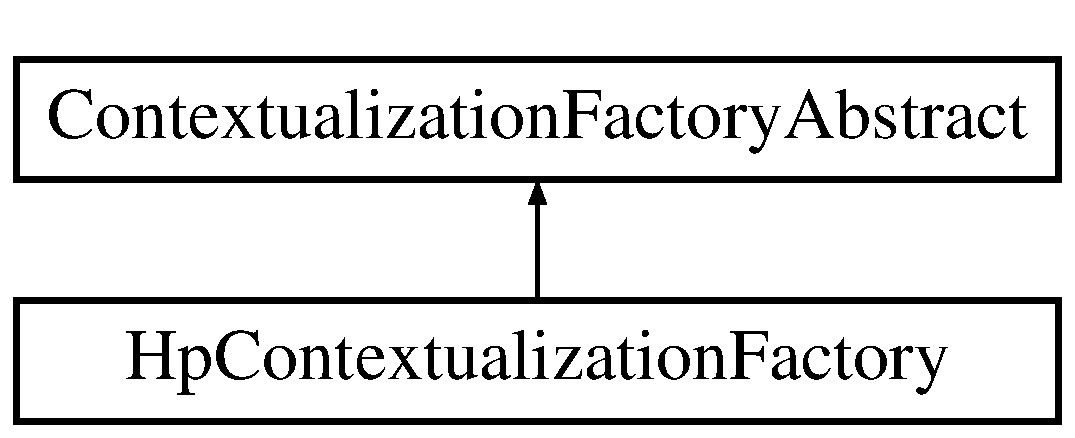
\includegraphics[height=2.000000cm]{classContextualizationFactoryAbstract}
\end{center}
\end{figure}
\subsection*{Public Types}
\begin{DoxyCompactItemize}
\item 
\mbox{\Hypertarget{classContextualizationFactoryAbstract_a87cd3e6ea2f582fe98286a73d3b28f60}\label{classContextualizationFactoryAbstract_a87cd3e6ea2f582fe98286a73d3b28f60}} 
enum \mbox{\hyperlink{classContextualizationFactoryAbstract_a87cd3e6ea2f582fe98286a73d3b28f60}{Kernel\+Type}} \{ {\bfseries Windows}, 
{\bfseries Linux}, 
{\bfseries Undefined}
 \}
\begin{DoxyCompactList}\small\item\em Kernel types for which Contextuation\+Controller are implemented. \end{DoxyCompactList}\end{DoxyCompactItemize}
\subsection*{Public Member Functions}
\begin{DoxyCompactItemize}
\item 
\mbox{\Hypertarget{classContextualizationFactoryAbstract_a5f3886dc42bb68d69c5ed39e204d982c}\label{classContextualizationFactoryAbstract_a5f3886dc42bb68d69c5ed39e204d982c}} 
\mbox{\hyperlink{classContextualizationFactoryAbstract_a5f3886dc42bb68d69c5ed39e204d982c}{Contextualization\+Factory\+Abstract}} ()
\begin{DoxyCompactList}\small\item\em Creates an empty \mbox{\hyperlink{classContextualizationFactoryAbstract}{Contextualization\+Factory\+Abstract}}. \end{DoxyCompactList}\item 
virtual \mbox{\hyperlink{classContextualizationController}{Contextualization\+Controller}} $\ast$ \mbox{\hyperlink{classContextualizationFactoryAbstract_a0898ad4d3a109c5767a1e596bf444e4a}{create\+Controller}} (char $\ast$$\ast$params, int count)=0
\begin{DoxyCompactList}\small\item\em Instantiates a new controller for a contextualization. \end{DoxyCompactList}\end{DoxyCompactItemize}
\subsection*{Protected Member Functions}
\begin{DoxyCompactItemize}
\item 
\mbox{\hyperlink{classContextualizationFactoryAbstract_a87cd3e6ea2f582fe98286a73d3b28f60}{Kernel\+Type}} \mbox{\hyperlink{classContextualizationFactoryAbstract_a2d7958c0f68ad388f832abcb7777397d}{get\+Current\+Kernel\+Type}} ()
\begin{DoxyCompactList}\small\item\em Returns the kernel type where the app is running. \end{DoxyCompactList}\end{DoxyCompactItemize}


\subsection{Detailed Description}
This is a interface factory to create a concrete class of \mbox{\hyperlink{classContextualizationController}{Contextualization\+Controller}}. 

Definition at line 17 of file contextualizationfactoryabstract.\+h.



\subsection{Member Function Documentation}
\mbox{\Hypertarget{classContextualizationFactoryAbstract_a0898ad4d3a109c5767a1e596bf444e4a}\label{classContextualizationFactoryAbstract_a0898ad4d3a109c5767a1e596bf444e4a}} 
\index{Contextualization\+Factory\+Abstract@{Contextualization\+Factory\+Abstract}!create\+Controller@{create\+Controller}}
\index{create\+Controller@{create\+Controller}!Contextualization\+Factory\+Abstract@{Contextualization\+Factory\+Abstract}}
\subsubsection{\texorpdfstring{create\+Controller()}{createController()}}
{\footnotesize\ttfamily virtual \mbox{\hyperlink{classContextualizationController}{Contextualization\+Controller}}$\ast$ Contextualization\+Factory\+Abstract\+::create\+Controller (\begin{DoxyParamCaption}\item[{char $\ast$$\ast$}]{params,  }\item[{int}]{count }\end{DoxyParamCaption})\hspace{0.3cm}{\ttfamily [pure virtual]}}



Instantiates a new controller for a contextualization. 

This is a pure vistual function that must to be implemented in inherits classes. 
\begin{DoxyParams}{Parameters}
{\em params} & Array params. \\
\hline
{\em count} & Number of elements of params. \\
\hline
\end{DoxyParams}
\begin{DoxyReturn}{Returns}
A new controller. 
\end{DoxyReturn}


Implemented in \mbox{\hyperlink{classHpContextualizationFactory_ad9d9c11a2827c8854c4cadbf38b4e7ca}{Hp\+Contextualization\+Factory}}.

\mbox{\Hypertarget{classContextualizationFactoryAbstract_a2d7958c0f68ad388f832abcb7777397d}\label{classContextualizationFactoryAbstract_a2d7958c0f68ad388f832abcb7777397d}} 
\index{Contextualization\+Factory\+Abstract@{Contextualization\+Factory\+Abstract}!get\+Current\+Kernel\+Type@{get\+Current\+Kernel\+Type}}
\index{get\+Current\+Kernel\+Type@{get\+Current\+Kernel\+Type}!Contextualization\+Factory\+Abstract@{Contextualization\+Factory\+Abstract}}
\subsubsection{\texorpdfstring{get\+Current\+Kernel\+Type()}{getCurrentKernelType()}}
{\footnotesize\ttfamily \mbox{\hyperlink{classContextualizationFactoryAbstract_a87cd3e6ea2f582fe98286a73d3b28f60}{Contextualization\+Factory\+Abstract\+::\+Kernel\+Type}} Contextualization\+Factory\+Abstract\+::get\+Current\+Kernel\+Type (\begin{DoxyParamCaption}{ }\end{DoxyParamCaption})\hspace{0.3cm}{\ttfamily [protected]}}



Returns the kernel type where the app is running. 

\begin{DoxyReturn}{Returns}
Kernel type of the current system. 
\end{DoxyReturn}


Definition at line 18 of file contextualizationfactoryabstract.\+cpp.



The documentation for this class was generated from the following files\+:\begin{DoxyCompactItemize}
\item 
src/tools/\mbox{\hyperlink{contextualizationfactoryabstract_8h}{contextualizationfactoryabstract.\+h}}\item 
src/tools/\mbox{\hyperlink{contextualizationfactoryabstract_8cpp}{contextualizationfactoryabstract.\+cpp}}\end{DoxyCompactItemize}

\hypertarget{classContextualizationModel}{}\section{Contextualization\+Model Class Reference}
\label{classContextualizationModel}\index{Contextualization\+Model@{Contextualization\+Model}}


This is the model class of a M\+VC architecture on Contextualization Tool app.  




{\ttfamily \#include $<$contextualizationmodel.\+h$>$}

Inheritance diagram for Contextualization\+Model\+:\begin{figure}[H]
\begin{center}
\leavevmode
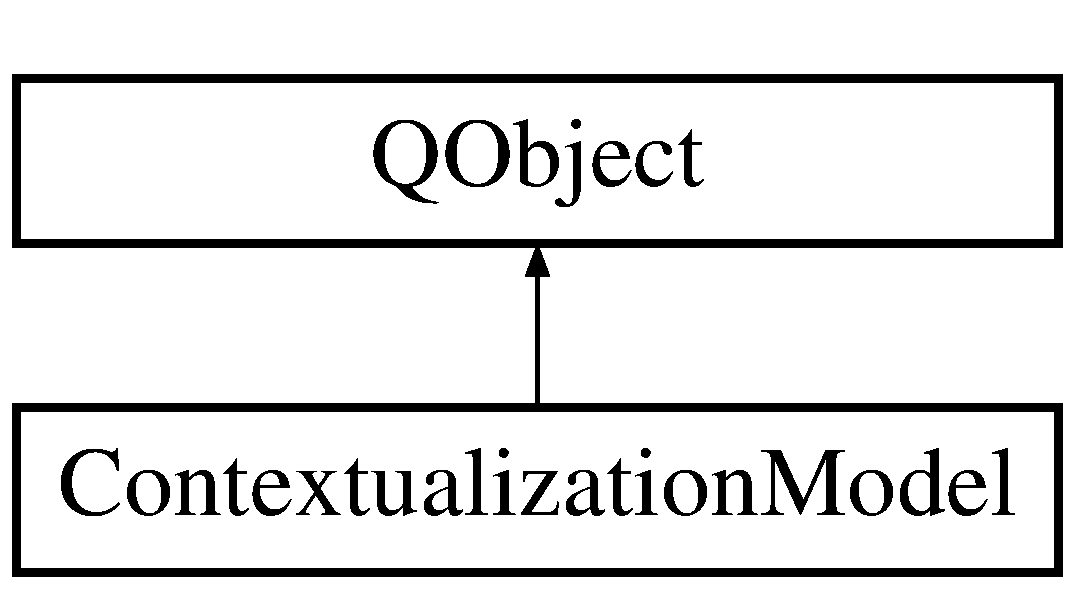
\includegraphics[height=2.000000cm]{classContextualizationModel}
\end{center}
\end{figure}
\subsection*{Signals}
\begin{DoxyCompactItemize}
\item 
\mbox{\Hypertarget{classContextualizationModel_a7b2878843e87cff00f5bce5bcb2d4949}\label{classContextualizationModel_a7b2878843e87cff00f5bce5bcb2d4949}} 
void \mbox{\hyperlink{classContextualizationModel_a7b2878843e87cff00f5bce5bcb2d4949}{strings\+List\+Changed}} ()
\begin{DoxyCompactList}\small\item\em This signal is emited when a string is modified on model. \end{DoxyCompactList}\item 
\mbox{\Hypertarget{classContextualizationModel_abc9b77f8362faea337fbd18fb25ee93a}\label{classContextualizationModel_abc9b77f8362faea337fbd18fb25ee93a}} 
void \mbox{\hyperlink{classContextualizationModel_abc9b77f8362faea337fbd18fb25ee93a}{image\+Changed}} ()
\begin{DoxyCompactList}\small\item\em This signal is emited when the image of model is changed. \end{DoxyCompactList}\end{DoxyCompactItemize}
\subsection*{Public Member Functions}
\begin{DoxyCompactItemize}
\item 
\mbox{\hyperlink{classContextualizationModel_a109126afb677af159e77adecf36fb6f2}{Contextualization\+Model}} (Q\+String image=\char`\"{}\char`\"{}, Q\+List$<$ \mbox{\hyperlink{classFirmwareString}{Firmware\+String}} $\ast$$>$ list=Q\+List$<$ \mbox{\hyperlink{classFirmwareString}{Firmware\+String}} $\ast$$>$())
\begin{DoxyCompactList}\small\item\em Constructs a model. \end{DoxyCompactList}\item 
\mbox{\Hypertarget{classContextualizationModel_a232b273faa1bdb051c7a7f61d6601370}\label{classContextualizationModel_a232b273faa1bdb051c7a7f61d6601370}} 
\mbox{\hyperlink{classContextualizationModel_a232b273faa1bdb051c7a7f61d6601370}{$\sim$\+Contextualization\+Model}} ()
\begin{DoxyCompactList}\small\item\em Destroys the model. \end{DoxyCompactList}\item 
void \mbox{\hyperlink{classContextualizationModel_aa87bafc64440304e8d9efd7f23f9b897}{add\+String}} (const Q\+String \&id, const Q\+String \&value, const Q\+String \&description, const Q\+String \&max\+Length, const Q\+String \&state, const bool selected)
\begin{DoxyCompactList}\small\item\em Adds new string to the model. \end{DoxyCompactList}\item 
void \mbox{\hyperlink{classContextualizationModel_aad4004198e03fb3e9bba770f0f76489e}{add\+String}} (\mbox{\hyperlink{classFirmwareString}{Firmware\+String}} $\ast$new\+String)
\begin{DoxyCompactList}\small\item\em Adds new string to the model. \end{DoxyCompactList}\item 
void \mbox{\hyperlink{classContextualizationModel_a24021cc16a5215c9765602b311fe9f77}{add\+Strings}} (Q\+List$<$ \mbox{\hyperlink{classFirmwareString}{Firmware\+String}} $\ast$$>$ \&strings)
\begin{DoxyCompactList}\small\item\em Adds new string to the model. \end{DoxyCompactList}\item 
bool \mbox{\hyperlink{classContextualizationModel_a65def773aab689eb131482834d711a22}{remove\+String}} (Q\+String \&id)
\begin{DoxyCompactList}\small\item\em Removes string with the identifier received by parameter. \end{DoxyCompactList}\item 
bool \mbox{\hyperlink{classContextualizationModel_a83ce3eb84747d052182a52b481314a85}{remove\+String}} (int pos)
\begin{DoxyCompactList}\small\item\em Removes string that are in position received by parameter. \end{DoxyCompactList}\item 
\mbox{\Hypertarget{classContextualizationModel_a09f646708d9dfaa87d064622a4776194}\label{classContextualizationModel_a09f646708d9dfaa87d064622a4776194}} 
void \mbox{\hyperlink{classContextualizationModel_a09f646708d9dfaa87d064622a4776194}{remove\+All\+Strings}} ()
\begin{DoxyCompactList}\small\item\em Removes all items from the firmware strings list. \end{DoxyCompactList}\item 
bool \mbox{\hyperlink{classContextualizationModel_a4aafa9c9e08d2b7a52b17871f755f34b}{select\+String}} (const Q\+String id)
\begin{DoxyCompactList}\small\item\em Selects string with the identifier received by parameter. \end{DoxyCompactList}\item 
bool \mbox{\hyperlink{classContextualizationModel_a7690c31f0c498607a8137d9d5acb3b32}{unselect\+String}} (const Q\+String id)
\begin{DoxyCompactList}\small\item\em Unselects string with the identifier received by parameter. \end{DoxyCompactList}\item 
Q\+List$<$ Q\+Object $\ast$ $>$ \& \mbox{\hyperlink{classContextualizationModel_ac098ebbf5cce5aac14182adddf7610e4}{get\+Strings\+List}} ()
\begin{DoxyCompactList}\small\item\em Returns the firmware strings list. \end{DoxyCompactList}\item 
void \mbox{\hyperlink{classContextualizationModel_a0d3ac87546d9b527c23cc69d0e4e0954}{set\+Image}} (Q\+String path)
\begin{DoxyCompactList}\small\item\em Sets the image of the model. \end{DoxyCompactList}\item 
Q\+String \mbox{\hyperlink{classContextualizationModel_a930b89fa044d406be44836cde09be11c}{get\+Image}} ()
\begin{DoxyCompactList}\small\item\em Returns the image associated to the model. \end{DoxyCompactList}\item 
bool \mbox{\hyperlink{classContextualizationModel_a0d5c107172b0d2e4026cae63d3193f4e}{is\+Empty}} ()
\begin{DoxyCompactList}\small\item\em Checks if the model is empty. \end{DoxyCompactList}\item 
bool \mbox{\hyperlink{classContextualizationModel_a47cf0c1ba3e6a86f264c501c9fb7e4e5}{has\+Image}} ()
\begin{DoxyCompactList}\small\item\em Returns true if the model has a valid image associated. \end{DoxyCompactList}\item 
bool \mbox{\hyperlink{classContextualizationModel_a369461aa31404ea4ff1c04fc2bd21f92}{has\+Strings}} ()
\begin{DoxyCompactList}\small\item\em Returns true if the model has any string. \end{DoxyCompactList}\item 
void \mbox{\hyperlink{classContextualizationModel_a17eeedb3696fd1d759761c0184d3dedc}{clear}} ()
\begin{DoxyCompactList}\small\item\em Empty the model. \end{DoxyCompactList}\item 
Q\+String \mbox{\hyperlink{classContextualizationModel_aeaea29193156f1c1d2a38a24de6ebbd5}{to\+Json}} (Q\+Json\+Document\+::\+Json\+Format format=Q\+Json\+Document\+::\+Compact)
\begin{DoxyCompactList}\small\item\em Returns the model converted to a J\+S\+ON Q\+String. \end{DoxyCompactList}\item 
Q\+Json\+Object \mbox{\hyperlink{classContextualizationModel_ac68d84aa77be188dfe51c850c0d5fd4e}{to\+Json\+Object}} ()
\begin{DoxyCompactList}\small\item\em Returns the model converted to a \#\+Q\+Json\+Object. \end{DoxyCompactList}\item 
\mbox{\hyperlink{classContextualizationModel}{Contextualization\+Model}} \& \mbox{\hyperlink{classContextualizationModel_a7c8d0dea4d32c2b573f1f58b0c01b81b}{operator=}} (\mbox{\hyperlink{classContextualizationModel}{Contextualization\+Model}} \&other)
\begin{DoxyCompactList}\small\item\em Assigns other to this model and returns a reference to this model. \end{DoxyCompactList}\end{DoxyCompactItemize}
\subsection*{Static Public Member Functions}
\begin{DoxyCompactItemize}
\item 
static \mbox{\hyperlink{classContextualizationModel}{Contextualization\+Model}} $\ast$ \mbox{\hyperlink{classContextualizationModel_aa334a054aa36564d56e812a1a9e6de30}{from\+Json}} (Q\+String \&json)
\begin{DoxyCompactList}\small\item\em Returns a \mbox{\hyperlink{classContextualizationModel}{Contextualization\+Model}} initializated with the J\+S\+ON string json. \end{DoxyCompactList}\item 
static \mbox{\hyperlink{classContextualizationModel}{Contextualization\+Model}} $\ast$ \mbox{\hyperlink{classContextualizationModel_a08ac67d6c9c3b949e9085d131fa47619}{from\+Json}} (Q\+Byte\+Array \&json)
\begin{DoxyCompactList}\small\item\em Returns a \mbox{\hyperlink{classContextualizationModel}{Contextualization\+Model}} initializated with the \#\+Q\+Byte\+Array data json. \end{DoxyCompactList}\end{DoxyCompactItemize}


\subsection{Detailed Description}
This is the model class of a M\+VC architecture on Contextualization Tool app. 

Definition at line 23 of file contextualizationmodel.\+h.



\subsection{Constructor \& Destructor Documentation}
\mbox{\Hypertarget{classContextualizationModel_a109126afb677af159e77adecf36fb6f2}\label{classContextualizationModel_a109126afb677af159e77adecf36fb6f2}} 
\index{Contextualization\+Model@{Contextualization\+Model}!Contextualization\+Model@{Contextualization\+Model}}
\index{Contextualization\+Model@{Contextualization\+Model}!Contextualization\+Model@{Contextualization\+Model}}
\subsubsection{\texorpdfstring{Contextualization\+Model()}{ContextualizationModel()}}
{\footnotesize\ttfamily Contextualization\+Model\+::\+Contextualization\+Model (\begin{DoxyParamCaption}\item[{Q\+String}]{image = {\ttfamily \char`\"{}\char`\"{}},  }\item[{Q\+List$<$ \mbox{\hyperlink{classFirmwareString}{Firmware\+String}} $\ast$$>$}]{list = {\ttfamily QList$<$\mbox{\hyperlink{classFirmwareString}{Firmware\+String}}~$\ast$$>$()} }\end{DoxyParamCaption})}



Constructs a model. 

Creates a model setting the image as the image received by parameter. Also adds to the model strings received in the list of the second parameter. If no parameters are received, create an empty model. 
\begin{DoxyParams}{Parameters}
{\em image} & File path of image to associate to the model. \\
\hline
{\em list} & List of strings to add on the model. \\
\hline
\end{DoxyParams}


Definition at line 13 of file contextualizationmodel.\+cpp.



\subsection{Member Function Documentation}
\mbox{\Hypertarget{classContextualizationModel_aa87bafc64440304e8d9efd7f23f9b897}\label{classContextualizationModel_aa87bafc64440304e8d9efd7f23f9b897}} 
\index{Contextualization\+Model@{Contextualization\+Model}!add\+String@{add\+String}}
\index{add\+String@{add\+String}!Contextualization\+Model@{Contextualization\+Model}}
\subsubsection{\texorpdfstring{add\+String()}{addString()}\hspace{0.1cm}{\footnotesize\ttfamily [1/2]}}
{\footnotesize\ttfamily void Contextualization\+Model\+::add\+String (\begin{DoxyParamCaption}\item[{const Q\+String \&}]{id,  }\item[{const Q\+String \&}]{value,  }\item[{const Q\+String \&}]{description,  }\item[{const Q\+String \&}]{max\+Length,  }\item[{const Q\+String \&}]{state,  }\item[{const bool}]{selected }\end{DoxyParamCaption})}



Adds new string to the model. 


\begin{DoxyParams}{Parameters}
{\em id} & \mbox{\hyperlink{classString}{String}} ID. \\
\hline
{\em value} & \mbox{\hyperlink{classString}{String}} value. \\
\hline
{\em description} & \mbox{\hyperlink{classString}{String}} description. \\
\hline
{\em max\+Length} & \mbox{\hyperlink{classString}{String}} max length. \\
\hline
{\em state} & \mbox{\hyperlink{classString}{String}} state. \\
\hline
{\em selected} & Indicates if the string is selected. \\
\hline
\end{DoxyParams}


Definition at line 30 of file contextualizationmodel.\+cpp.

\mbox{\Hypertarget{classContextualizationModel_aad4004198e03fb3e9bba770f0f76489e}\label{classContextualizationModel_aad4004198e03fb3e9bba770f0f76489e}} 
\index{Contextualization\+Model@{Contextualization\+Model}!add\+String@{add\+String}}
\index{add\+String@{add\+String}!Contextualization\+Model@{Contextualization\+Model}}
\subsubsection{\texorpdfstring{add\+String()}{addString()}\hspace{0.1cm}{\footnotesize\ttfamily [2/2]}}
{\footnotesize\ttfamily void Contextualization\+Model\+::add\+String (\begin{DoxyParamCaption}\item[{\mbox{\hyperlink{classFirmwareString}{Firmware\+String}} $\ast$}]{new\+String }\end{DoxyParamCaption})}



Adds new string to the model. 


\begin{DoxyParams}{Parameters}
{\em new\+String} & \\
\hline
\end{DoxyParams}


Definition at line 42 of file contextualizationmodel.\+cpp.

\mbox{\Hypertarget{classContextualizationModel_a24021cc16a5215c9765602b311fe9f77}\label{classContextualizationModel_a24021cc16a5215c9765602b311fe9f77}} 
\index{Contextualization\+Model@{Contextualization\+Model}!add\+Strings@{add\+Strings}}
\index{add\+Strings@{add\+Strings}!Contextualization\+Model@{Contextualization\+Model}}
\subsubsection{\texorpdfstring{add\+Strings()}{addStrings()}}
{\footnotesize\ttfamily void Contextualization\+Model\+::add\+Strings (\begin{DoxyParamCaption}\item[{Q\+List$<$ \mbox{\hyperlink{classFirmwareString}{Firmware\+String}} $\ast$$>$ \&}]{strings }\end{DoxyParamCaption})}



Adds new string to the model. 

Adds all strings in the list received by parameter. 
\begin{DoxyParams}{Parameters}
{\em strings} & List of strings to add. \\
\hline
\end{DoxyParams}


Definition at line 49 of file contextualizationmodel.\+cpp.

\mbox{\Hypertarget{classContextualizationModel_a17eeedb3696fd1d759761c0184d3dedc}\label{classContextualizationModel_a17eeedb3696fd1d759761c0184d3dedc}} 
\index{Contextualization\+Model@{Contextualization\+Model}!clear@{clear}}
\index{clear@{clear}!Contextualization\+Model@{Contextualization\+Model}}
\subsubsection{\texorpdfstring{clear()}{clear()}}
{\footnotesize\ttfamily void Contextualization\+Model\+::clear (\begin{DoxyParamCaption}{ }\end{DoxyParamCaption})}



Empty the model. 

Unsets the path of image and removes all items from the firmware strings list. 

Definition at line 179 of file contextualizationmodel.\+cpp.

\mbox{\Hypertarget{classContextualizationModel_aa334a054aa36564d56e812a1a9e6de30}\label{classContextualizationModel_aa334a054aa36564d56e812a1a9e6de30}} 
\index{Contextualization\+Model@{Contextualization\+Model}!from\+Json@{from\+Json}}
\index{from\+Json@{from\+Json}!Contextualization\+Model@{Contextualization\+Model}}
\subsubsection{\texorpdfstring{from\+Json()}{fromJson()}\hspace{0.1cm}{\footnotesize\ttfamily [1/2]}}
{\footnotesize\ttfamily \mbox{\hyperlink{classContextualizationModel}{Contextualization\+Model}} $\ast$ Contextualization\+Model\+::from\+Json (\begin{DoxyParamCaption}\item[{Q\+String \&}]{json }\end{DoxyParamCaption})\hspace{0.3cm}{\ttfamily [static]}}



Returns a \mbox{\hyperlink{classContextualizationModel}{Contextualization\+Model}} initializated with the J\+S\+ON string json. 

If the J\+S\+ON data received is not valid, return an empty model. 
\begin{DoxyParams}{Parameters}
{\em json} & \mbox{\hyperlink{classString}{String}} in J\+S\+ON format to be converted. \\
\hline
\end{DoxyParams}
\begin{DoxyReturn}{Returns}
\mbox{\hyperlink{classContextualizationModel}{Contextualization\+Model}} 
\end{DoxyReturn}


Definition at line 207 of file contextualizationmodel.\+cpp.

\mbox{\Hypertarget{classContextualizationModel_a08ac67d6c9c3b949e9085d131fa47619}\label{classContextualizationModel_a08ac67d6c9c3b949e9085d131fa47619}} 
\index{Contextualization\+Model@{Contextualization\+Model}!from\+Json@{from\+Json}}
\index{from\+Json@{from\+Json}!Contextualization\+Model@{Contextualization\+Model}}
\subsubsection{\texorpdfstring{from\+Json()}{fromJson()}\hspace{0.1cm}{\footnotesize\ttfamily [2/2]}}
{\footnotesize\ttfamily \mbox{\hyperlink{classContextualizationModel}{Contextualization\+Model}} $\ast$ Contextualization\+Model\+::from\+Json (\begin{DoxyParamCaption}\item[{Q\+Byte\+Array \&}]{json }\end{DoxyParamCaption})\hspace{0.3cm}{\ttfamily [static]}}



Returns a \mbox{\hyperlink{classContextualizationModel}{Contextualization\+Model}} initializated with the \#\+Q\+Byte\+Array data json. 

If the J\+S\+ON data received is not valid, return an empty model. 
\begin{DoxyParams}{Parameters}
{\em json} & Q\+Byte\+Array in J\+S\+ON format to be converted. \\
\hline
\end{DoxyParams}
\begin{DoxyReturn}{Returns}
\mbox{\hyperlink{classContextualizationModel}{Contextualization\+Model}} 
\end{DoxyReturn}
$<$ Release memory because of an error on json decode process. 

Definition at line 214 of file contextualizationmodel.\+cpp.

\mbox{\Hypertarget{classContextualizationModel_a930b89fa044d406be44836cde09be11c}\label{classContextualizationModel_a930b89fa044d406be44836cde09be11c}} 
\index{Contextualization\+Model@{Contextualization\+Model}!get\+Image@{get\+Image}}
\index{get\+Image@{get\+Image}!Contextualization\+Model@{Contextualization\+Model}}
\subsubsection{\texorpdfstring{get\+Image()}{getImage()}}
{\footnotesize\ttfamily Q\+String Contextualization\+Model\+::get\+Image (\begin{DoxyParamCaption}{ }\end{DoxyParamCaption})}



Returns the image associated to the model. 

\begin{DoxyReturn}{Returns}
Q\+String 
\end{DoxyReturn}


Definition at line 155 of file contextualizationmodel.\+cpp.

\mbox{\Hypertarget{classContextualizationModel_ac098ebbf5cce5aac14182adddf7610e4}\label{classContextualizationModel_ac098ebbf5cce5aac14182adddf7610e4}} 
\index{Contextualization\+Model@{Contextualization\+Model}!get\+Strings\+List@{get\+Strings\+List}}
\index{get\+Strings\+List@{get\+Strings\+List}!Contextualization\+Model@{Contextualization\+Model}}
\subsubsection{\texorpdfstring{get\+Strings\+List()}{getStringsList()}}
{\footnotesize\ttfamily Q\+List$<$ Q\+Object $\ast$ $>$ \& Contextualization\+Model\+::get\+Strings\+List (\begin{DoxyParamCaption}{ }\end{DoxyParamCaption})}



Returns the firmware strings list. 

\begin{DoxyReturn}{Returns}
Q\+List$<$\+Firmware\+String $\ast$$>$ \& 
\end{DoxyReturn}


Definition at line 141 of file contextualizationmodel.\+cpp.

\mbox{\Hypertarget{classContextualizationModel_a47cf0c1ba3e6a86f264c501c9fb7e4e5}\label{classContextualizationModel_a47cf0c1ba3e6a86f264c501c9fb7e4e5}} 
\index{Contextualization\+Model@{Contextualization\+Model}!has\+Image@{has\+Image}}
\index{has\+Image@{has\+Image}!Contextualization\+Model@{Contextualization\+Model}}
\subsubsection{\texorpdfstring{has\+Image()}{hasImage()}}
{\footnotesize\ttfamily bool Contextualization\+Model\+::has\+Image (\begin{DoxyParamCaption}{ }\end{DoxyParamCaption})}



Returns true if the model has a valid image associated. 

\begin{DoxyReturn}{Returns}
bool 
\end{DoxyReturn}


Definition at line 169 of file contextualizationmodel.\+cpp.

\mbox{\Hypertarget{classContextualizationModel_a369461aa31404ea4ff1c04fc2bd21f92}\label{classContextualizationModel_a369461aa31404ea4ff1c04fc2bd21f92}} 
\index{Contextualization\+Model@{Contextualization\+Model}!has\+Strings@{has\+Strings}}
\index{has\+Strings@{has\+Strings}!Contextualization\+Model@{Contextualization\+Model}}
\subsubsection{\texorpdfstring{has\+Strings()}{hasStrings()}}
{\footnotesize\ttfamily bool Contextualization\+Model\+::has\+Strings (\begin{DoxyParamCaption}{ }\end{DoxyParamCaption})}



Returns true if the model has any string. 

\begin{DoxyReturn}{Returns}
bool. 
\end{DoxyReturn}


Definition at line 174 of file contextualizationmodel.\+cpp.

\mbox{\Hypertarget{classContextualizationModel_a0d5c107172b0d2e4026cae63d3193f4e}\label{classContextualizationModel_a0d5c107172b0d2e4026cae63d3193f4e}} 
\index{Contextualization\+Model@{Contextualization\+Model}!is\+Empty@{is\+Empty}}
\index{is\+Empty@{is\+Empty}!Contextualization\+Model@{Contextualization\+Model}}
\subsubsection{\texorpdfstring{is\+Empty()}{isEmpty()}}
{\footnotesize\ttfamily bool Contextualization\+Model\+::is\+Empty (\begin{DoxyParamCaption}{ }\end{DoxyParamCaption})}



Checks if the model is empty. 

The model is empty when there aren\textquotesingle{}t any image in the model and the firmware strings list is empty. Return true if model is empty. \begin{DoxyReturn}{Returns}

\end{DoxyReturn}


Definition at line 160 of file contextualizationmodel.\+cpp.

\mbox{\Hypertarget{classContextualizationModel_a7c8d0dea4d32c2b573f1f58b0c01b81b}\label{classContextualizationModel_a7c8d0dea4d32c2b573f1f58b0c01b81b}} 
\index{Contextualization\+Model@{Contextualization\+Model}!operator=@{operator=}}
\index{operator=@{operator=}!Contextualization\+Model@{Contextualization\+Model}}
\subsubsection{\texorpdfstring{operator=()}{operator=()}}
{\footnotesize\ttfamily \mbox{\hyperlink{classContextualizationModel}{Contextualization\+Model}} \& Contextualization\+Model\+::operator= (\begin{DoxyParamCaption}\item[{\mbox{\hyperlink{classContextualizationModel}{Contextualization\+Model}} \&}]{other }\end{DoxyParamCaption})}



Assigns other to this model and returns a reference to this model. 


\begin{DoxyParams}{Parameters}
{\em other} & Model to be copied. \\
\hline
\end{DoxyParams}
\begin{DoxyReturn}{Returns}
Reference to this model. 
\end{DoxyReturn}


Definition at line 269 of file contextualizationmodel.\+cpp.

\mbox{\Hypertarget{classContextualizationModel_a65def773aab689eb131482834d711a22}\label{classContextualizationModel_a65def773aab689eb131482834d711a22}} 
\index{Contextualization\+Model@{Contextualization\+Model}!remove\+String@{remove\+String}}
\index{remove\+String@{remove\+String}!Contextualization\+Model@{Contextualization\+Model}}
\subsubsection{\texorpdfstring{remove\+String()}{removeString()}\hspace{0.1cm}{\footnotesize\ttfamily [1/2]}}
{\footnotesize\ttfamily bool Contextualization\+Model\+::remove\+String (\begin{DoxyParamCaption}\item[{Q\+String \&}]{id }\end{DoxyParamCaption})}



Removes string with the identifier received by parameter. 

Returns true if the string removed succesfuly. Returns false if there are not any string with this identifer. 
\begin{DoxyParams}{Parameters}
{\em id} & Identifier of firmware string to remove. \\
\hline
\end{DoxyParams}
\begin{DoxyReturn}{Returns}
bool 
\end{DoxyReturn}


Definition at line 56 of file contextualizationmodel.\+cpp.

\mbox{\Hypertarget{classContextualizationModel_a83ce3eb84747d052182a52b481314a85}\label{classContextualizationModel_a83ce3eb84747d052182a52b481314a85}} 
\index{Contextualization\+Model@{Contextualization\+Model}!remove\+String@{remove\+String}}
\index{remove\+String@{remove\+String}!Contextualization\+Model@{Contextualization\+Model}}
\subsubsection{\texorpdfstring{remove\+String()}{removeString()}\hspace{0.1cm}{\footnotesize\ttfamily [2/2]}}
{\footnotesize\ttfamily bool Contextualization\+Model\+::remove\+String (\begin{DoxyParamCaption}\item[{int}]{pos }\end{DoxyParamCaption})}



Removes string that are in position received by parameter. 

Returns true if the string removed succesfuly. Returns false if is not a valid position. 
\begin{DoxyParams}{Parameters}
{\em pos} & Position of the string in list. \\
\hline
\end{DoxyParams}
\begin{DoxyReturn}{Returns}
bool 
\end{DoxyReturn}


Definition at line 75 of file contextualizationmodel.\+cpp.

\mbox{\Hypertarget{classContextualizationModel_a4aafa9c9e08d2b7a52b17871f755f34b}\label{classContextualizationModel_a4aafa9c9e08d2b7a52b17871f755f34b}} 
\index{Contextualization\+Model@{Contextualization\+Model}!select\+String@{select\+String}}
\index{select\+String@{select\+String}!Contextualization\+Model@{Contextualization\+Model}}
\subsubsection{\texorpdfstring{select\+String()}{selectString()}}
{\footnotesize\ttfamily bool Contextualization\+Model\+::select\+String (\begin{DoxyParamCaption}\item[{const Q\+String}]{id }\end{DoxyParamCaption})}



Selects string with the identifier received by parameter. 

Returns true if the string selected succesfuly. Returns false if there are not any string with this identifer. 
\begin{DoxyParams}{Parameters}
{\em id} & Identifier of firmware string to remove. \\
\hline
\end{DoxyParams}
\begin{DoxyReturn}{Returns}
bool 
\end{DoxyReturn}


Definition at line 105 of file contextualizationmodel.\+cpp.

\mbox{\Hypertarget{classContextualizationModel_a0d3ac87546d9b527c23cc69d0e4e0954}\label{classContextualizationModel_a0d3ac87546d9b527c23cc69d0e4e0954}} 
\index{Contextualization\+Model@{Contextualization\+Model}!set\+Image@{set\+Image}}
\index{set\+Image@{set\+Image}!Contextualization\+Model@{Contextualization\+Model}}
\subsubsection{\texorpdfstring{set\+Image()}{setImage()}}
{\footnotesize\ttfamily void Contextualization\+Model\+::set\+Image (\begin{DoxyParamCaption}\item[{Q\+String}]{path }\end{DoxyParamCaption})}



Sets the image of the model. 


\begin{DoxyParams}{Parameters}
{\em path} & File path of the image. \\
\hline
\end{DoxyParams}


Definition at line 146 of file contextualizationmodel.\+cpp.

\mbox{\Hypertarget{classContextualizationModel_aeaea29193156f1c1d2a38a24de6ebbd5}\label{classContextualizationModel_aeaea29193156f1c1d2a38a24de6ebbd5}} 
\index{Contextualization\+Model@{Contextualization\+Model}!to\+Json@{to\+Json}}
\index{to\+Json@{to\+Json}!Contextualization\+Model@{Contextualization\+Model}}
\subsubsection{\texorpdfstring{to\+Json()}{toJson()}}
{\footnotesize\ttfamily Q\+String Contextualization\+Model\+::to\+Json (\begin{DoxyParamCaption}\item[{Q\+Json\+Document\+::\+Json\+Format}]{format = {\ttfamily QJsonDocument\+:\+:Compact} }\end{DoxyParamCaption})}



Returns the model converted to a J\+S\+ON Q\+String. 


\begin{DoxyParams}{Parameters}
{\em format} & Exit format of J\+S\+ON. \\
\hline
\end{DoxyParams}
\begin{DoxyReturn}{Returns}
Q\+String 
\end{DoxyReturn}


Definition at line 185 of file contextualizationmodel.\+cpp.

\mbox{\Hypertarget{classContextualizationModel_ac68d84aa77be188dfe51c850c0d5fd4e}\label{classContextualizationModel_ac68d84aa77be188dfe51c850c0d5fd4e}} 
\index{Contextualization\+Model@{Contextualization\+Model}!to\+Json\+Object@{to\+Json\+Object}}
\index{to\+Json\+Object@{to\+Json\+Object}!Contextualization\+Model@{Contextualization\+Model}}
\subsubsection{\texorpdfstring{to\+Json\+Object()}{toJsonObject()}}
{\footnotesize\ttfamily Q\+Json\+Object Contextualization\+Model\+::to\+Json\+Object (\begin{DoxyParamCaption}{ }\end{DoxyParamCaption})}



Returns the model converted to a \#\+Q\+Json\+Object. 

\begin{DoxyReturn}{Returns}
Q\+Json\+Object 
\end{DoxyReturn}


Definition at line 190 of file contextualizationmodel.\+cpp.

\mbox{\Hypertarget{classContextualizationModel_a7690c31f0c498607a8137d9d5acb3b32}\label{classContextualizationModel_a7690c31f0c498607a8137d9d5acb3b32}} 
\index{Contextualization\+Model@{Contextualization\+Model}!unselect\+String@{unselect\+String}}
\index{unselect\+String@{unselect\+String}!Contextualization\+Model@{Contextualization\+Model}}
\subsubsection{\texorpdfstring{unselect\+String()}{unselectString()}}
{\footnotesize\ttfamily bool Contextualization\+Model\+::unselect\+String (\begin{DoxyParamCaption}\item[{const Q\+String}]{id }\end{DoxyParamCaption})}



Unselects string with the identifier received by parameter. 

Returns true if the string selected succesfuly. Returns false if there are not any string with this identifer. 
\begin{DoxyParams}{Parameters}
{\em id} & Identifier of firmware string to remove. \\
\hline
\end{DoxyParams}
\begin{DoxyReturn}{Returns}
bool 
\end{DoxyReturn}


Definition at line 123 of file contextualizationmodel.\+cpp.



The documentation for this class was generated from the following files\+:\begin{DoxyCompactItemize}
\item 
src/contextualization/model/\mbox{\hyperlink{contextualizationmodel_8h}{contextualizationmodel.\+h}}\item 
src/contextualization/model/\mbox{\hyperlink{contextualizationmodel_8cpp}{contextualizationmodel.\+cpp}}\end{DoxyCompactItemize}

\hypertarget{classDatabaseConnectorAbstract}{}\section{Database\+Connector\+Abstract Class Reference}
\label{classDatabaseConnectorAbstract}\index{Database\+Connector\+Abstract@{Database\+Connector\+Abstract}}


This is an interface to access a different data bases.  




{\ttfamily \#include $<$databaseconnectorabstract.\+h$>$}

Inheritance diagram for Database\+Connector\+Abstract\+:\begin{figure}[H]
\begin{center}
\leavevmode
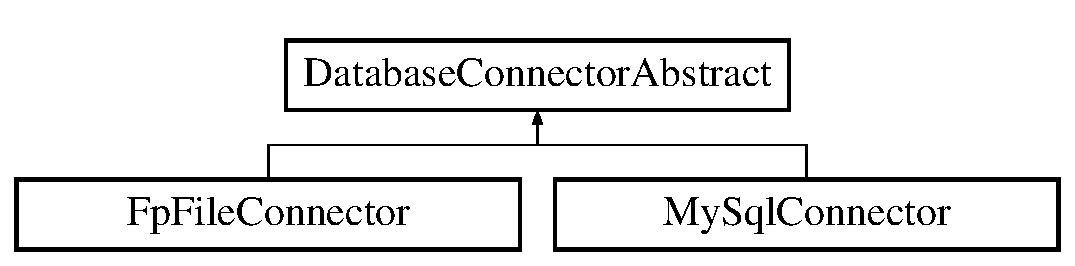
\includegraphics[height=2.000000cm]{classDatabaseConnectorAbstract}
\end{center}
\end{figure}
\subsection*{Public Member Functions}
\begin{DoxyCompactItemize}
\item 
\mbox{\Hypertarget{classDatabaseConnectorAbstract_a0a5f40156183723e5e01d5ab50418118}\label{classDatabaseConnectorAbstract_a0a5f40156183723e5e01d5ab50418118}} 
\mbox{\hyperlink{classDatabaseConnectorAbstract_a0a5f40156183723e5e01d5ab50418118}{Database\+Connector\+Abstract}} ()
\begin{DoxyCompactList}\small\item\em Creates an empty \mbox{\hyperlink{classDatabaseConnectorAbstract}{Database\+Connector\+Abstract}}. \end{DoxyCompactList}\item 
virtual Q\+List$<$ \mbox{\hyperlink{classString}{String}} $\ast$ $>$ \mbox{\hyperlink{classDatabaseConnectorAbstract_aeb4347bc18b6bed9a9b6120f68c10e9d}{get\+All\+Strings}} ()=0
\begin{DoxyCompactList}\small\item\em Returns a list containing all strings in the dababase. \end{DoxyCompactList}\item 
virtual Q\+List$<$ \mbox{\hyperlink{classString}{String}} $\ast$ $>$ \mbox{\hyperlink{classDatabaseConnectorAbstract_a1d33547045c5f8619f44290c932edb1b}{get\+Strings\+With\+Value}} (const Q\+String \&value, bool case\+Sensitive=true)=0
\begin{DoxyCompactList}\small\item\em Returns all strigns in database with the value received by argument. \end{DoxyCompactList}\item 
virtual Q\+List$<$ \mbox{\hyperlink{classString}{String}} $\ast$ $>$ \mbox{\hyperlink{classDatabaseConnectorAbstract_a5b0f30372ca105a94073267e969b74ee}{get\+Strings\+With\+Approximate\+Value}} (const Q\+String \&value, bool case\+Sensitive=true)=0
\begin{DoxyCompactList}\small\item\em Returns all strigns in database with a similar value received by argument. \end{DoxyCompactList}\item 
virtual Q\+List$<$ \mbox{\hyperlink{classString}{String}} $\ast$ $>$ \mbox{\hyperlink{classDatabaseConnectorAbstract_a757f25feaf50af012d25db8f27b1fef4}{get\+String\+With\+Id}} (const Q\+String \&id, bool case\+Sensitive=true)=0
\begin{DoxyCompactList}\small\item\em Returns all strigns in database with the identifier received by argument. \end{DoxyCompactList}\item 
virtual Q\+List$<$ \mbox{\hyperlink{classString}{String}} $\ast$ $>$ \mbox{\hyperlink{classDatabaseConnectorAbstract_a74952c7e14c891e33c84995066003c5a}{get\+Strings\+With\+State}} (const Q\+String state)=0
\begin{DoxyCompactList}\small\item\em Returns strings with state received by parameter. \end{DoxyCompactList}\item 
virtual bool \mbox{\hyperlink{classDatabaseConnectorAbstract_ac7cc5cf2deace9652810001722758206}{insert\+String}} (const \mbox{\hyperlink{classString}{String}} \&string, const Q\+String language)=0
\begin{DoxyCompactList}\small\item\em Inserts a new string in database. \end{DoxyCompactList}\item 
virtual int \mbox{\hyperlink{classDatabaseConnectorAbstract_a0e8c94cf0b38c797d6feef864a23347b}{insert\+Strings}} (const Q\+List$<$ \mbox{\hyperlink{classString}{String}} $\ast$$>$ \&strings, const Q\+String language)=0
\begin{DoxyCompactList}\small\item\em Inserts a set of strings into the database. \end{DoxyCompactList}\item 
virtual int \mbox{\hyperlink{classDatabaseConnectorAbstract_af482c0b4af4488c5897c04d0c4dff906}{remove\+Strings\+With\+Value}} (const Q\+String \&value, bool case\+Sensitive=true)=0
\begin{DoxyCompactList}\small\item\em Removes from databse all strigns with the value received by argument. \end{DoxyCompactList}\item 
virtual int \mbox{\hyperlink{classDatabaseConnectorAbstract_a8c2b0fa4e37d16c1b1ea1cafec166ca0}{remove\+Strings\+With\+Id}} (const Q\+String \&id, bool case\+Sensitive=true)=0
\begin{DoxyCompactList}\small\item\em Removes from databse the strign with the identifier received by argument. \end{DoxyCompactList}\item 
virtual Q\+String\+List \mbox{\hyperlink{classDatabaseConnectorAbstract_a77ff263d407366e54f3e8512c575ff5e}{get\+Languages}} ()=0
\begin{DoxyCompactList}\small\item\em Returns all languages stored in database. \end{DoxyCompactList}\item 
virtual Q\+String\+List \mbox{\hyperlink{classDatabaseConnectorAbstract_a98f5b2472bab6edc82ce2c5554319d7f}{get\+Language\+Ids}} ()=0
\begin{DoxyCompactList}\small\item\em Returns all language identifiers stored in database. \end{DoxyCompactList}\end{DoxyCompactItemize}
\subsection*{Protected Attributes}
\begin{DoxyCompactItemize}
\item 
\mbox{\Hypertarget{classDatabaseConnectorAbstract_a1ab06cd87949b36d40d4a26d0fc22ff3}\label{classDatabaseConnectorAbstract_a1ab06cd87949b36d40d4a26d0fc22ff3}} 
const int \mbox{\hyperlink{classDatabaseConnectorAbstract_a1ab06cd87949b36d40d4a26d0fc22ff3}{M\+I\+N\+\_\+\+L\+E\+N\+G\+T\+H\+\_\+\+F\+O\+R\+\_\+\+A\+P\+P\+R\+O\+X\+I\+M\+A\+TE}}
\begin{DoxyCompactList}\small\item\em Minimun length for string to do an approximate find. \end{DoxyCompactList}\item 
\mbox{\Hypertarget{classDatabaseConnectorAbstract_acb4ab89c1daae4bd7a252677fb87f66e}\label{classDatabaseConnectorAbstract_acb4ab89c1daae4bd7a252677fb87f66e}} 
const int \mbox{\hyperlink{classDatabaseConnectorAbstract_acb4ab89c1daae4bd7a252677fb87f66e}{M\+A\+X\+\_\+\+L\+E\+N\+G\+T\+H\+\_\+\+D\+I\+F\+F\+E\+R\+E\+N\+CE}}
\begin{DoxyCompactList}\small\item\em Greatest difference between value and string values found. \end{DoxyCompactList}\end{DoxyCompactItemize}


\subsection{Detailed Description}
This is an interface to access a different data bases. 

Definition at line 18 of file databaseconnectorabstract.\+h.



\subsection{Member Function Documentation}
\mbox{\Hypertarget{classDatabaseConnectorAbstract_aeb4347bc18b6bed9a9b6120f68c10e9d}\label{classDatabaseConnectorAbstract_aeb4347bc18b6bed9a9b6120f68c10e9d}} 
\index{Database\+Connector\+Abstract@{Database\+Connector\+Abstract}!get\+All\+Strings@{get\+All\+Strings}}
\index{get\+All\+Strings@{get\+All\+Strings}!Database\+Connector\+Abstract@{Database\+Connector\+Abstract}}
\subsubsection{\texorpdfstring{get\+All\+Strings()}{getAllStrings()}}
{\footnotesize\ttfamily virtual Q\+List$<$\mbox{\hyperlink{classString}{String}} $\ast$$>$ Database\+Connector\+Abstract\+::get\+All\+Strings (\begin{DoxyParamCaption}{ }\end{DoxyParamCaption})\hspace{0.3cm}{\ttfamily [pure virtual]}}



Returns a list containing all strings in the dababase. 

\begin{DoxyReturn}{Returns}
List with strings. 
\end{DoxyReturn}


Implemented in \mbox{\hyperlink{classMySqlConnector_ad6ff79c4049e3631800da97e8d7b7704}{My\+Sql\+Connector}}, and \mbox{\hyperlink{classFpFileConnector_ad392db922a5e04a670b84fc616192eea}{Fp\+File\+Connector}}.

\mbox{\Hypertarget{classDatabaseConnectorAbstract_a98f5b2472bab6edc82ce2c5554319d7f}\label{classDatabaseConnectorAbstract_a98f5b2472bab6edc82ce2c5554319d7f}} 
\index{Database\+Connector\+Abstract@{Database\+Connector\+Abstract}!get\+Language\+Ids@{get\+Language\+Ids}}
\index{get\+Language\+Ids@{get\+Language\+Ids}!Database\+Connector\+Abstract@{Database\+Connector\+Abstract}}
\subsubsection{\texorpdfstring{get\+Language\+Ids()}{getLanguageIds()}}
{\footnotesize\ttfamily virtual Q\+String\+List Database\+Connector\+Abstract\+::get\+Language\+Ids (\begin{DoxyParamCaption}{ }\end{DoxyParamCaption})\hspace{0.3cm}{\ttfamily [pure virtual]}}



Returns all language identifiers stored in database. 

\begin{DoxyReturn}{Returns}
Languages used. 
\end{DoxyReturn}


Implemented in \mbox{\hyperlink{classMySqlConnector_a3493828360c7edd217461e040fc1b00e}{My\+Sql\+Connector}}, and \mbox{\hyperlink{classFpFileConnector_a290016844ec3093b1c58db33fc86cd0a}{Fp\+File\+Connector}}.

\mbox{\Hypertarget{classDatabaseConnectorAbstract_a77ff263d407366e54f3e8512c575ff5e}\label{classDatabaseConnectorAbstract_a77ff263d407366e54f3e8512c575ff5e}} 
\index{Database\+Connector\+Abstract@{Database\+Connector\+Abstract}!get\+Languages@{get\+Languages}}
\index{get\+Languages@{get\+Languages}!Database\+Connector\+Abstract@{Database\+Connector\+Abstract}}
\subsubsection{\texorpdfstring{get\+Languages()}{getLanguages()}}
{\footnotesize\ttfamily virtual Q\+String\+List Database\+Connector\+Abstract\+::get\+Languages (\begin{DoxyParamCaption}{ }\end{DoxyParamCaption})\hspace{0.3cm}{\ttfamily [pure virtual]}}



Returns all languages stored in database. 

\begin{DoxyReturn}{Returns}
Languages used. 
\end{DoxyReturn}


Implemented in \mbox{\hyperlink{classMySqlConnector_a83be1a4d67e509b6604629660eb7c4a0}{My\+Sql\+Connector}}, and \mbox{\hyperlink{classFpFileConnector_a82b6ae6887737cfea3b982cb0874424e}{Fp\+File\+Connector}}.

\mbox{\Hypertarget{classDatabaseConnectorAbstract_a5b0f30372ca105a94073267e969b74ee}\label{classDatabaseConnectorAbstract_a5b0f30372ca105a94073267e969b74ee}} 
\index{Database\+Connector\+Abstract@{Database\+Connector\+Abstract}!get\+Strings\+With\+Approximate\+Value@{get\+Strings\+With\+Approximate\+Value}}
\index{get\+Strings\+With\+Approximate\+Value@{get\+Strings\+With\+Approximate\+Value}!Database\+Connector\+Abstract@{Database\+Connector\+Abstract}}
\subsubsection{\texorpdfstring{get\+Strings\+With\+Approximate\+Value()}{getStringsWithApproximateValue()}}
{\footnotesize\ttfamily virtual Q\+List$<$\mbox{\hyperlink{classString}{String}} $\ast$$>$ Database\+Connector\+Abstract\+::get\+Strings\+With\+Approximate\+Value (\begin{DoxyParamCaption}\item[{const Q\+String \&}]{value,  }\item[{bool}]{case\+Sensitive = {\ttfamily true} }\end{DoxyParamCaption})\hspace{0.3cm}{\ttfamily [pure virtual]}}



Returns all strigns in database with a similar value received by argument. 


\begin{DoxyParams}{Parameters}
{\em value} & \mbox{\hyperlink{classString}{String}} value. \\
\hline
\end{DoxyParams}
\begin{DoxyReturn}{Returns}
List with strings. 
\end{DoxyReturn}


Implemented in \mbox{\hyperlink{classMySqlConnector_a8a480141c72dc8da687b15f921ab1a4e}{My\+Sql\+Connector}}, and \mbox{\hyperlink{classFpFileConnector_adc85e526e1dab9f3de03cb8a2f33f7d1}{Fp\+File\+Connector}}.

\mbox{\Hypertarget{classDatabaseConnectorAbstract_a74952c7e14c891e33c84995066003c5a}\label{classDatabaseConnectorAbstract_a74952c7e14c891e33c84995066003c5a}} 
\index{Database\+Connector\+Abstract@{Database\+Connector\+Abstract}!get\+Strings\+With\+State@{get\+Strings\+With\+State}}
\index{get\+Strings\+With\+State@{get\+Strings\+With\+State}!Database\+Connector\+Abstract@{Database\+Connector\+Abstract}}
\subsubsection{\texorpdfstring{get\+Strings\+With\+State()}{getStringsWithState()}}
{\footnotesize\ttfamily virtual Q\+List$<$\mbox{\hyperlink{classString}{String}} $\ast$$>$ Database\+Connector\+Abstract\+::get\+Strings\+With\+State (\begin{DoxyParamCaption}\item[{const Q\+String}]{state }\end{DoxyParamCaption})\hspace{0.3cm}{\ttfamily [pure virtual]}}



Returns strings with state received by parameter. 


\begin{DoxyParams}{Parameters}
{\em state} & State to be found. \\
\hline
\end{DoxyParams}
\begin{DoxyReturn}{Returns}
\mbox{\hyperlink{classString}{String}} list eith indicated state. 
\end{DoxyReturn}


Implemented in \mbox{\hyperlink{classMySqlConnector_a821c3dcebcd763df1700881cb47685d5}{My\+Sql\+Connector}}, and \mbox{\hyperlink{classFpFileConnector_a4c671329fd2fd1b9c3a7d72de1028afd}{Fp\+File\+Connector}}.

\mbox{\Hypertarget{classDatabaseConnectorAbstract_a1d33547045c5f8619f44290c932edb1b}\label{classDatabaseConnectorAbstract_a1d33547045c5f8619f44290c932edb1b}} 
\index{Database\+Connector\+Abstract@{Database\+Connector\+Abstract}!get\+Strings\+With\+Value@{get\+Strings\+With\+Value}}
\index{get\+Strings\+With\+Value@{get\+Strings\+With\+Value}!Database\+Connector\+Abstract@{Database\+Connector\+Abstract}}
\subsubsection{\texorpdfstring{get\+Strings\+With\+Value()}{getStringsWithValue()}}
{\footnotesize\ttfamily virtual Q\+List$<$\mbox{\hyperlink{classString}{String}} $\ast$$>$ Database\+Connector\+Abstract\+::get\+Strings\+With\+Value (\begin{DoxyParamCaption}\item[{const Q\+String \&}]{value,  }\item[{bool}]{case\+Sensitive = {\ttfamily true} }\end{DoxyParamCaption})\hspace{0.3cm}{\ttfamily [pure virtual]}}



Returns all strigns in database with the value received by argument. 


\begin{DoxyParams}{Parameters}
{\em value} & \mbox{\hyperlink{classString}{String}} value. \\
\hline
\end{DoxyParams}
\begin{DoxyReturn}{Returns}
List with strings. 
\end{DoxyReturn}


Implemented in \mbox{\hyperlink{classMySqlConnector_ae7440816a5bda9e63ea526656c4001f5}{My\+Sql\+Connector}}, and \mbox{\hyperlink{classFpFileConnector_a72a6ca5a5b8a44783d2ed990b111675b}{Fp\+File\+Connector}}.

\mbox{\Hypertarget{classDatabaseConnectorAbstract_a757f25feaf50af012d25db8f27b1fef4}\label{classDatabaseConnectorAbstract_a757f25feaf50af012d25db8f27b1fef4}} 
\index{Database\+Connector\+Abstract@{Database\+Connector\+Abstract}!get\+String\+With\+Id@{get\+String\+With\+Id}}
\index{get\+String\+With\+Id@{get\+String\+With\+Id}!Database\+Connector\+Abstract@{Database\+Connector\+Abstract}}
\subsubsection{\texorpdfstring{get\+String\+With\+Id()}{getStringWithId()}}
{\footnotesize\ttfamily virtual Q\+List$<$\mbox{\hyperlink{classString}{String}} $\ast$$>$ Database\+Connector\+Abstract\+::get\+String\+With\+Id (\begin{DoxyParamCaption}\item[{const Q\+String \&}]{id,  }\item[{bool}]{case\+Sensitive = {\ttfamily true} }\end{DoxyParamCaption})\hspace{0.3cm}{\ttfamily [pure virtual]}}



Returns all strigns in database with the identifier received by argument. 


\begin{DoxyParams}{Parameters}
{\em value} & \mbox{\hyperlink{classString}{String}} identifier. \\
\hline
\end{DoxyParams}
\begin{DoxyReturn}{Returns}
List with strings. 
\end{DoxyReturn}


Implemented in \mbox{\hyperlink{classMySqlConnector_a269bbced50451ff0ce48cfc4f2bb6a3b}{My\+Sql\+Connector}}, and \mbox{\hyperlink{classFpFileConnector_a29a6df6ea88a1e44f6b04c600b45925c}{Fp\+File\+Connector}}.

\mbox{\Hypertarget{classDatabaseConnectorAbstract_ac7cc5cf2deace9652810001722758206}\label{classDatabaseConnectorAbstract_ac7cc5cf2deace9652810001722758206}} 
\index{Database\+Connector\+Abstract@{Database\+Connector\+Abstract}!insert\+String@{insert\+String}}
\index{insert\+String@{insert\+String}!Database\+Connector\+Abstract@{Database\+Connector\+Abstract}}
\subsubsection{\texorpdfstring{insert\+String()}{insertString()}}
{\footnotesize\ttfamily virtual bool Database\+Connector\+Abstract\+::insert\+String (\begin{DoxyParamCaption}\item[{const \mbox{\hyperlink{classString}{String}} \&}]{string,  }\item[{const Q\+String}]{language }\end{DoxyParamCaption})\hspace{0.3cm}{\ttfamily [pure virtual]}}



Inserts a new string in database. 

Returns true if the insertion was succesfull, otherwise, returns false. 
\begin{DoxyParams}{Parameters}
{\em string} & \mbox{\hyperlink{classString}{String}} instance to be inserted. \\
\hline
\end{DoxyParams}
\begin{DoxyReturn}{Returns}
bool 
\end{DoxyReturn}


Implemented in \mbox{\hyperlink{classMySqlConnector_a4608c0764241969454a55b42873cb86b}{My\+Sql\+Connector}}, and \mbox{\hyperlink{classFpFileConnector_ae4f79d6a1281a20702b0257de56822b2}{Fp\+File\+Connector}}.

\mbox{\Hypertarget{classDatabaseConnectorAbstract_a0e8c94cf0b38c797d6feef864a23347b}\label{classDatabaseConnectorAbstract_a0e8c94cf0b38c797d6feef864a23347b}} 
\index{Database\+Connector\+Abstract@{Database\+Connector\+Abstract}!insert\+Strings@{insert\+Strings}}
\index{insert\+Strings@{insert\+Strings}!Database\+Connector\+Abstract@{Database\+Connector\+Abstract}}
\subsubsection{\texorpdfstring{insert\+Strings()}{insertStrings()}}
{\footnotesize\ttfamily virtual int Database\+Connector\+Abstract\+::insert\+Strings (\begin{DoxyParamCaption}\item[{const Q\+List$<$ \mbox{\hyperlink{classString}{String}} $\ast$$>$ \&}]{strings,  }\item[{const Q\+String}]{language }\end{DoxyParamCaption})\hspace{0.3cm}{\ttfamily [pure virtual]}}



Inserts a set of strings into the database. 

Returns the number of inserted stirngs. 
\begin{DoxyParams}{Parameters}
{\em strings} & List with strings to be added into databse. \\
\hline
\end{DoxyParams}
\begin{DoxyReturn}{Returns}
bool 
\end{DoxyReturn}


Implemented in \mbox{\hyperlink{classMySqlConnector_a77a5169dd8a515b613642c88dac9798b}{My\+Sql\+Connector}}, and \mbox{\hyperlink{classFpFileConnector_a7f31d3e699ce4c489c2303370d032a7e}{Fp\+File\+Connector}}.

\mbox{\Hypertarget{classDatabaseConnectorAbstract_a8c2b0fa4e37d16c1b1ea1cafec166ca0}\label{classDatabaseConnectorAbstract_a8c2b0fa4e37d16c1b1ea1cafec166ca0}} 
\index{Database\+Connector\+Abstract@{Database\+Connector\+Abstract}!remove\+Strings\+With\+Id@{remove\+Strings\+With\+Id}}
\index{remove\+Strings\+With\+Id@{remove\+Strings\+With\+Id}!Database\+Connector\+Abstract@{Database\+Connector\+Abstract}}
\subsubsection{\texorpdfstring{remove\+Strings\+With\+Id()}{removeStringsWithId()}}
{\footnotesize\ttfamily virtual int Database\+Connector\+Abstract\+::remove\+Strings\+With\+Id (\begin{DoxyParamCaption}\item[{const Q\+String \&}]{id,  }\item[{bool}]{case\+Sensitive = {\ttfamily true} }\end{DoxyParamCaption})\hspace{0.3cm}{\ttfamily [pure virtual]}}



Removes from databse the strign with the identifier received by argument. 

Returns the number of removed stirngs. 
\begin{DoxyParams}{Parameters}
{\em value} & \mbox{\hyperlink{classString}{String}} identifier. \\
\hline
\end{DoxyParams}
\begin{DoxyReturn}{Returns}
bool 
\end{DoxyReturn}


Implemented in \mbox{\hyperlink{classMySqlConnector_a3c340e5310c56410d64ecd89e5cf6661}{My\+Sql\+Connector}}, and \mbox{\hyperlink{classFpFileConnector_a8e09804b3c21f6b56dcc70659bbf105f}{Fp\+File\+Connector}}.

\mbox{\Hypertarget{classDatabaseConnectorAbstract_af482c0b4af4488c5897c04d0c4dff906}\label{classDatabaseConnectorAbstract_af482c0b4af4488c5897c04d0c4dff906}} 
\index{Database\+Connector\+Abstract@{Database\+Connector\+Abstract}!remove\+Strings\+With\+Value@{remove\+Strings\+With\+Value}}
\index{remove\+Strings\+With\+Value@{remove\+Strings\+With\+Value}!Database\+Connector\+Abstract@{Database\+Connector\+Abstract}}
\subsubsection{\texorpdfstring{remove\+Strings\+With\+Value()}{removeStringsWithValue()}}
{\footnotesize\ttfamily virtual int Database\+Connector\+Abstract\+::remove\+Strings\+With\+Value (\begin{DoxyParamCaption}\item[{const Q\+String \&}]{value,  }\item[{bool}]{case\+Sensitive = {\ttfamily true} }\end{DoxyParamCaption})\hspace{0.3cm}{\ttfamily [pure virtual]}}



Removes from databse all strigns with the value received by argument. 

Returns the number of removed strings. 
\begin{DoxyParams}{Parameters}
{\em value} & \mbox{\hyperlink{classString}{String}} value. \\
\hline
\end{DoxyParams}
\begin{DoxyReturn}{Returns}
Number of removed strings 
\end{DoxyReturn}


Implemented in \mbox{\hyperlink{classMySqlConnector_a528aac591ea56ade27a096bb997abb2a}{My\+Sql\+Connector}}, and \mbox{\hyperlink{classFpFileConnector_a57c6eafd6b4c7dfbd927f6d4cb63d25c}{Fp\+File\+Connector}}.



The documentation for this class was generated from the following files\+:\begin{DoxyCompactItemize}
\item 
src/storage/\mbox{\hyperlink{databaseconnectorabstract_8h}{databaseconnectorabstract.\+h}}\item 
src/storage/\mbox{\hyperlink{databaseconnectorabstract_8cpp}{databaseconnectorabstract.\+cpp}}\end{DoxyCompactItemize}

\hypertarget{classFirmwareString}{}\section{Firmware\+String Class Reference}
\label{classFirmwareString}\index{Firmware\+String@{Firmware\+String}}


This a representation of a Firmware \mbox{\hyperlink{classString}{String}} used in HP company.  




{\ttfamily \#include $<$firmwarestring.\+h$>$}

Inheritance diagram for Firmware\+String\+:\begin{figure}[H]
\begin{center}
\leavevmode
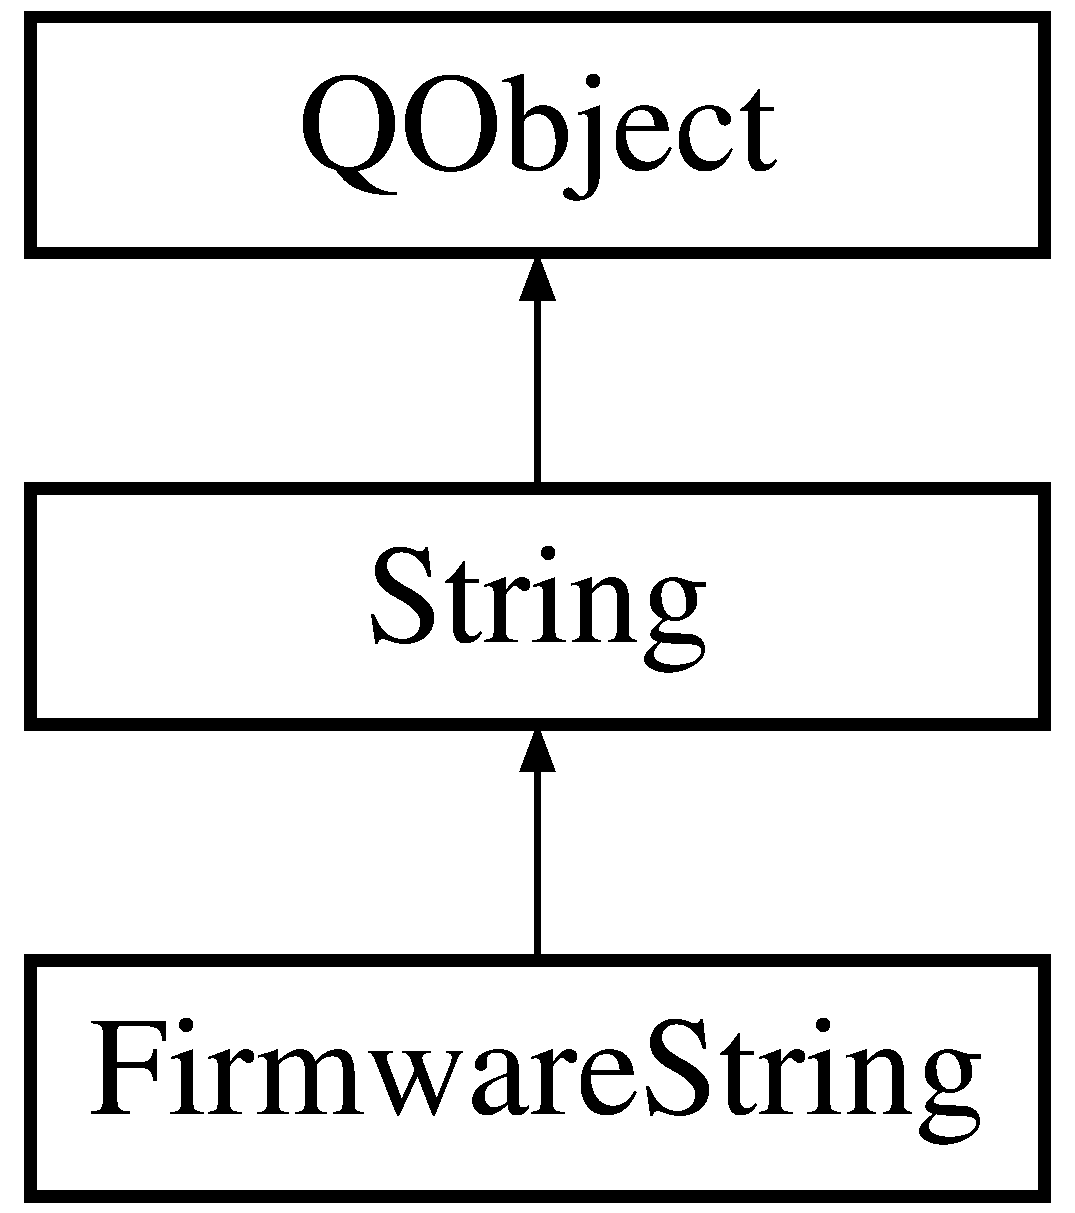
\includegraphics[height=3.000000cm]{classFirmwareString}
\end{center}
\end{figure}
\subsection*{Public Member Functions}
\begin{DoxyCompactItemize}
\item 
\mbox{\hyperlink{classFirmwareString_a624ab9d3c534ffd9c99665d2462e73ac}{Firmware\+String}} ()
\begin{DoxyCompactList}\small\item\em Constructs an empty string. \end{DoxyCompactList}\item 
\mbox{\hyperlink{classFirmwareString_a3439d83bad2ac371123d26560f4f3716}{Firmware\+String}} (\mbox{\hyperlink{classFirmwareString}{Firmware\+String}} \&other)
\begin{DoxyCompactList}\small\item\em Constructs a string replic from another received by parameter. \end{DoxyCompactList}\item 
\mbox{\hyperlink{classFirmwareString_a29f14882ef2a8274cebb7d153f0ea85b}{Firmware\+String}} (const Q\+String \&id, const Q\+String \&value, const Q\+String \&description, const Q\+String \&max\+Length, const Q\+String \&state, const bool selected=false, const bool editable=false)
\begin{DoxyCompactList}\small\item\em Constructs a firmware string with diferents value members received by parameter. \end{DoxyCompactList}\item 
\mbox{\hyperlink{classFirmwareString}{Firmware\+String}} \& \mbox{\hyperlink{classFirmwareString_aa2fe115e019e6362ca1fb151097ffe88}{operator=}} (const \mbox{\hyperlink{classFirmwareString}{Firmware\+String}} \&other)
\begin{DoxyCompactList}\small\item\em Assigns other to firmware string and returns a reference to this firmware string. \end{DoxyCompactList}\end{DoxyCompactItemize}
\subsection*{Static Public Member Functions}
\begin{DoxyCompactItemize}
\item 
static \mbox{\hyperlink{classFirmwareString}{Firmware\+String}} $\ast$ \mbox{\hyperlink{classFirmwareString_a94293dec7077d625c6b977f1f15bfd2d}{from\+Json}} (Q\+String \&json)
\begin{DoxyCompactList}\small\item\em Returns a \mbox{\hyperlink{classString}{String}} initializated with the J\+S\+ON string json. \end{DoxyCompactList}\item 
static \mbox{\hyperlink{classFirmwareString}{Firmware\+String}} $\ast$ \mbox{\hyperlink{classFirmwareString_a90a6e343748d41c0a0ab9eb7e4fccaee}{from\+Json}} (Q\+Byte\+Array \&json)
\begin{DoxyCompactList}\small\item\em Returns a \mbox{\hyperlink{classString}{String}} initializated with the \#\+Q\+Byte\+Array data json. \end{DoxyCompactList}\item 
static \mbox{\hyperlink{classFirmwareString}{Firmware\+String}} $\ast$ \mbox{\hyperlink{classFirmwareString_a0fcfdf14bbecd7c2c4464574b9ce9d91}{from\+Fp\+Line}} (const Q\+String \&fp\+Line)
\begin{DoxyCompactList}\small\item\em Converts a line of fp file in a \mbox{\hyperlink{classFirmwareString}{Firmware\+String}} if is possible. \end{DoxyCompactList}\end{DoxyCompactItemize}
\subsection*{Additional Inherited Members}


\subsection{Detailed Description}
This a representation of a Firmware \mbox{\hyperlink{classString}{String}} used in HP company. 

Definition at line 16 of file firmwarestring.\+h.



\subsection{Constructor \& Destructor Documentation}
\mbox{\Hypertarget{classFirmwareString_a624ab9d3c534ffd9c99665d2462e73ac}\label{classFirmwareString_a624ab9d3c534ffd9c99665d2462e73ac}} 
\index{Firmware\+String@{Firmware\+String}!Firmware\+String@{Firmware\+String}}
\index{Firmware\+String@{Firmware\+String}!Firmware\+String@{Firmware\+String}}
\subsubsection{\texorpdfstring{Firmware\+String()}{FirmwareString()}\hspace{0.1cm}{\footnotesize\ttfamily [1/3]}}
{\footnotesize\ttfamily Firmware\+String\+::\+Firmware\+String (\begin{DoxyParamCaption}{ }\end{DoxyParamCaption})}



Constructs an empty string. 



Definition at line 13 of file firmwarestring.\+cpp.

\mbox{\Hypertarget{classFirmwareString_a3439d83bad2ac371123d26560f4f3716}\label{classFirmwareString_a3439d83bad2ac371123d26560f4f3716}} 
\index{Firmware\+String@{Firmware\+String}!Firmware\+String@{Firmware\+String}}
\index{Firmware\+String@{Firmware\+String}!Firmware\+String@{Firmware\+String}}
\subsubsection{\texorpdfstring{Firmware\+String()}{FirmwareString()}\hspace{0.1cm}{\footnotesize\ttfamily [2/3]}}
{\footnotesize\ttfamily Firmware\+String\+::\+Firmware\+String (\begin{DoxyParamCaption}\item[{\mbox{\hyperlink{classFirmwareString}{Firmware\+String}} \&}]{other }\end{DoxyParamCaption})}



Constructs a string replic from another received by parameter. 


\begin{DoxyParams}{Parameters}
{\em other} & string to be duplicated. \\
\hline
\end{DoxyParams}


Definition at line 18 of file firmwarestring.\+cpp.

\mbox{\Hypertarget{classFirmwareString_a29f14882ef2a8274cebb7d153f0ea85b}\label{classFirmwareString_a29f14882ef2a8274cebb7d153f0ea85b}} 
\index{Firmware\+String@{Firmware\+String}!Firmware\+String@{Firmware\+String}}
\index{Firmware\+String@{Firmware\+String}!Firmware\+String@{Firmware\+String}}
\subsubsection{\texorpdfstring{Firmware\+String()}{FirmwareString()}\hspace{0.1cm}{\footnotesize\ttfamily [3/3]}}
{\footnotesize\ttfamily Firmware\+String\+::\+Firmware\+String (\begin{DoxyParamCaption}\item[{const Q\+String \&}]{id,  }\item[{const Q\+String \&}]{value,  }\item[{const Q\+String \&}]{description,  }\item[{const Q\+String \&}]{max\+Length,  }\item[{const Q\+String \&}]{state,  }\item[{const bool}]{selected = {\ttfamily false},  }\item[{const bool}]{editable = {\ttfamily false} }\end{DoxyParamCaption})}



Constructs a firmware string with diferents value members received by parameter. 


\begin{DoxyParams}{Parameters}
{\em id} & Firmware string identifier. \\
\hline
{\em value} & Firmware string value. \\
\hline
{\em description} & Firmware string description. \\
\hline
{\em max\+Length} & Firmware string max\+Length. \\
\hline
{\em state} & Firmware string state. \\
\hline
{\em selected} & Firmware string selected. \\
\hline
\end{DoxyParams}


Definition at line 29 of file firmwarestring.\+cpp.



\subsection{Member Function Documentation}
\mbox{\Hypertarget{classFirmwareString_a0fcfdf14bbecd7c2c4464574b9ce9d91}\label{classFirmwareString_a0fcfdf14bbecd7c2c4464574b9ce9d91}} 
\index{Firmware\+String@{Firmware\+String}!from\+Fp\+Line@{from\+Fp\+Line}}
\index{from\+Fp\+Line@{from\+Fp\+Line}!Firmware\+String@{Firmware\+String}}
\subsubsection{\texorpdfstring{from\+Fp\+Line()}{fromFpLine()}}
{\footnotesize\ttfamily \mbox{\hyperlink{classFirmwareString}{Firmware\+String}} $\ast$ Firmware\+String\+::from\+Fp\+Line (\begin{DoxyParamCaption}\item[{const Q\+String \&}]{fp\+Line }\end{DoxyParamCaption})\hspace{0.3cm}{\ttfamily [static]}}



Converts a line of fp file in a \mbox{\hyperlink{classFirmwareString}{Firmware\+String}} if is possible. 

Return null if there is a format error in the line. 
\begin{DoxyParams}{Parameters}
{\em line} & Contains string to fragment. \\
\hline
{\em line\+Number} & Contains the number of line on the file. \\
\hline
\end{DoxyParams}
\begin{DoxyReturn}{Returns}
\mbox{\hyperlink{classFirmwareString}{Firmware\+String}} $\ast$$\vert$null 
\end{DoxyReturn}


Definition at line 51 of file firmwarestring.\+cpp.

\mbox{\Hypertarget{classFirmwareString_a94293dec7077d625c6b977f1f15bfd2d}\label{classFirmwareString_a94293dec7077d625c6b977f1f15bfd2d}} 
\index{Firmware\+String@{Firmware\+String}!from\+Json@{from\+Json}}
\index{from\+Json@{from\+Json}!Firmware\+String@{Firmware\+String}}
\subsubsection{\texorpdfstring{from\+Json()}{fromJson()}\hspace{0.1cm}{\footnotesize\ttfamily [1/2]}}
{\footnotesize\ttfamily \mbox{\hyperlink{classFirmwareString}{Firmware\+String}} $\ast$ Firmware\+String\+::from\+Json (\begin{DoxyParamCaption}\item[{Q\+String \&}]{json }\end{DoxyParamCaption})\hspace{0.3cm}{\ttfamily [static]}}



Returns a \mbox{\hyperlink{classString}{String}} initializated with the J\+S\+ON string json. 

If the J\+S\+ON data received is not valid, return an empty model. 
\begin{DoxyParams}{Parameters}
{\em json} & \mbox{\hyperlink{classString}{String}} in J\+S\+ON format to be converted. \\
\hline
\end{DoxyParams}
\begin{DoxyReturn}{Returns}
\mbox{\hyperlink{classContextualizationModel}{Contextualization\+Model}} 
\end{DoxyReturn}


Definition at line 41 of file firmwarestring.\+cpp.

\mbox{\Hypertarget{classFirmwareString_a90a6e343748d41c0a0ab9eb7e4fccaee}\label{classFirmwareString_a90a6e343748d41c0a0ab9eb7e4fccaee}} 
\index{Firmware\+String@{Firmware\+String}!from\+Json@{from\+Json}}
\index{from\+Json@{from\+Json}!Firmware\+String@{Firmware\+String}}
\subsubsection{\texorpdfstring{from\+Json()}{fromJson()}\hspace{0.1cm}{\footnotesize\ttfamily [2/2]}}
{\footnotesize\ttfamily \mbox{\hyperlink{classFirmwareString}{Firmware\+String}} $\ast$ Firmware\+String\+::from\+Json (\begin{DoxyParamCaption}\item[{Q\+Byte\+Array \&}]{json }\end{DoxyParamCaption})\hspace{0.3cm}{\ttfamily [static]}}



Returns a \mbox{\hyperlink{classString}{String}} initializated with the \#\+Q\+Byte\+Array data json. 

If the J\+S\+ON data received is not valid, return an empty model. 
\begin{DoxyParams}{Parameters}
{\em json} & Q\+Byte\+Array in J\+S\+ON format to be converted. \\
\hline
\end{DoxyParams}
\begin{DoxyReturn}{Returns}
\mbox{\hyperlink{classString}{String}} 
\end{DoxyReturn}


Definition at line 46 of file firmwarestring.\+cpp.

\mbox{\Hypertarget{classFirmwareString_aa2fe115e019e6362ca1fb151097ffe88}\label{classFirmwareString_aa2fe115e019e6362ca1fb151097ffe88}} 
\index{Firmware\+String@{Firmware\+String}!operator=@{operator=}}
\index{operator=@{operator=}!Firmware\+String@{Firmware\+String}}
\subsubsection{\texorpdfstring{operator=()}{operator=()}}
{\footnotesize\ttfamily \mbox{\hyperlink{classFirmwareString}{Firmware\+String}} \& Firmware\+String\+::operator= (\begin{DoxyParamCaption}\item[{const \mbox{\hyperlink{classFirmwareString}{Firmware\+String}} \&}]{other }\end{DoxyParamCaption})}



Assigns other to firmware string and returns a reference to this firmware string. 


\begin{DoxyParams}{Parameters}
{\em other} & Model to be copied. \\
\hline
\end{DoxyParams}
\begin{DoxyReturn}{Returns}
Reference to this firmware string. 
\end{DoxyReturn}


Definition at line 119 of file firmwarestring.\+cpp.



The documentation for this class was generated from the following files\+:\begin{DoxyCompactItemize}
\item 
src/contextualization/model/\mbox{\hyperlink{firmwarestring_8h}{firmwarestring.\+h}}\item 
src/contextualization/model/\mbox{\hyperlink{firmwarestring_8cpp}{firmwarestring.\+cpp}}\end{DoxyCompactItemize}

\hypertarget{classFpFileConnector}{}\section{Fp\+File\+Connector Class Reference}
\label{classFpFileConnector}\index{Fp\+File\+Connector@{Fp\+File\+Connector}}


This is a class to access a database saved as fp file by HP company.  




{\ttfamily \#include $<$fpfileconnector.\+h$>$}

Inheritance diagram for Fp\+File\+Connector\+:\begin{figure}[H]
\begin{center}
\leavevmode
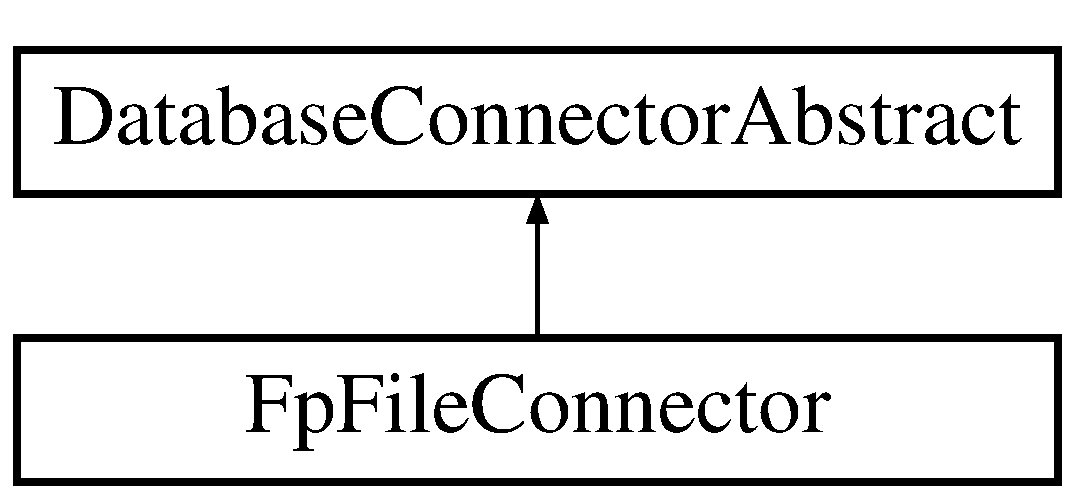
\includegraphics[height=2.000000cm]{classFpFileConnector}
\end{center}
\end{figure}
\subsection*{Public Member Functions}
\begin{DoxyCompactItemize}
\item 
\mbox{\Hypertarget{classFpFileConnector_a2e474f8746dd54729fe68c224ff24275}\label{classFpFileConnector_a2e474f8746dd54729fe68c224ff24275}} 
\mbox{\hyperlink{classFpFileConnector_a2e474f8746dd54729fe68c224ff24275}{Fp\+File\+Connector}} ()
\begin{DoxyCompactList}\small\item\em Creates an empty \mbox{\hyperlink{classFpFileConnector}{Fp\+File\+Connector}}. \end{DoxyCompactList}\item 
\mbox{\hyperlink{classFpFileConnector_a51b38b735ab4728601aef295d7b4c21f}{Fp\+File\+Connector}} (const Q\+String \&path)
\begin{DoxyCompactList}\small\item\em Creates a \mbox{\hyperlink{classFpFileConnector}{Fp\+File\+Connector}} and sets the path of file. \end{DoxyCompactList}\item 
Q\+String \mbox{\hyperlink{classFpFileConnector_af1a00dabd759abd0b59bf9e26edc73cf}{get\+Path}} ()
\begin{DoxyCompactList}\small\item\em Returns a path of database file. \end{DoxyCompactList}\item 
bool \mbox{\hyperlink{classFpFileConnector_a7a5c2987feae762ce359de702f5702e3}{set\+Path}} (const Q\+String \&path)
\begin{DoxyCompactList}\small\item\em Sets the path of database file. \end{DoxyCompactList}\item 
Q\+List$<$ \mbox{\hyperlink{classString}{String}} $\ast$ $>$ \mbox{\hyperlink{classFpFileConnector_ad392db922a5e04a670b84fc616192eea}{get\+All\+Strings}} () override
\item 
Q\+List$<$ \mbox{\hyperlink{classString}{String}} $\ast$ $>$ \mbox{\hyperlink{classFpFileConnector_a72a6ca5a5b8a44783d2ed990b111675b}{get\+Strings\+With\+Value}} (const Q\+String \&value, bool case\+Sensitive=true) override
\begin{DoxyCompactList}\small\item\em Returns all strigns in database with the value received by argument. \end{DoxyCompactList}\item 
Q\+List$<$ \mbox{\hyperlink{classString}{String}} $\ast$ $>$ \mbox{\hyperlink{classFpFileConnector_adc85e526e1dab9f3de03cb8a2f33f7d1}{get\+Strings\+With\+Approximate\+Value}} (const Q\+String \&value, bool case\+Sensitive=true) override
\begin{DoxyCompactList}\small\item\em Returns all strigns in database with a similar value received by argument. \end{DoxyCompactList}\item 
Q\+List$<$ \mbox{\hyperlink{classString}{String}} $\ast$ $>$ \mbox{\hyperlink{classFpFileConnector_a29a6df6ea88a1e44f6b04c600b45925c}{get\+String\+With\+Id}} (const Q\+String \&id, bool case\+Sensitive=true) override
\begin{DoxyCompactList}\small\item\em Returns all strigns in database with the identifier received by argument. \end{DoxyCompactList}\item 
Q\+List$<$ \mbox{\hyperlink{classString}{String}} $\ast$ $>$ \mbox{\hyperlink{classFpFileConnector_a4c671329fd2fd1b9c3a7d72de1028afd}{get\+Strings\+With\+State}} (const Q\+String state) override
\begin{DoxyCompactList}\small\item\em Returns strings with state received by parameter. \end{DoxyCompactList}\item 
bool \mbox{\hyperlink{classFpFileConnector_ae4f79d6a1281a20702b0257de56822b2}{insert\+String}} (const \mbox{\hyperlink{classString}{String}} \&string, const Q\+String language=Q\+String()) override
\begin{DoxyCompactList}\small\item\em Inserts a new string in database. \end{DoxyCompactList}\item 
int \mbox{\hyperlink{classFpFileConnector_a7f31d3e699ce4c489c2303370d032a7e}{insert\+Strings}} (const Q\+List$<$ \mbox{\hyperlink{classString}{String}} $\ast$$>$ \&strings, const Q\+String language=Q\+String()) override
\begin{DoxyCompactList}\small\item\em Inserts a set of strings into the database. \end{DoxyCompactList}\item 
int \mbox{\hyperlink{classFpFileConnector_a57c6eafd6b4c7dfbd927f6d4cb63d25c}{remove\+Strings\+With\+Value}} (const Q\+String \&value, bool case\+Sensitive=true) override
\begin{DoxyCompactList}\small\item\em Removes from databse all strigns with the value received by argument. \end{DoxyCompactList}\item 
int \mbox{\hyperlink{classFpFileConnector_a8e09804b3c21f6b56dcc70659bbf105f}{remove\+Strings\+With\+Id}} (const Q\+String \&id, bool case\+Sensitive=true) override
\begin{DoxyCompactList}\small\item\em Removes from databse the strign with the identifier received by argument. \end{DoxyCompactList}\item 
Q\+String\+List \mbox{\hyperlink{classFpFileConnector_a82b6ae6887737cfea3b982cb0874424e}{get\+Languages}} () override
\begin{DoxyCompactList}\small\item\em Returns all languages stored in database. \end{DoxyCompactList}\item 
Q\+String\+List \mbox{\hyperlink{classFpFileConnector_a290016844ec3093b1c58db33fc86cd0a}{get\+Language\+Ids}} () override
\begin{DoxyCompactList}\small\item\em Returns all language identifiers stored in database. \end{DoxyCompactList}\end{DoxyCompactItemize}
\subsection*{Additional Inherited Members}


\subsection{Detailed Description}
This is a class to access a database saved as fp file by HP company. 

Definition at line 21 of file fpfileconnector.\+h.



\subsection{Constructor \& Destructor Documentation}
\mbox{\Hypertarget{classFpFileConnector_a51b38b735ab4728601aef295d7b4c21f}\label{classFpFileConnector_a51b38b735ab4728601aef295d7b4c21f}} 
\index{Fp\+File\+Connector@{Fp\+File\+Connector}!Fp\+File\+Connector@{Fp\+File\+Connector}}
\index{Fp\+File\+Connector@{Fp\+File\+Connector}!Fp\+File\+Connector@{Fp\+File\+Connector}}
\subsubsection{\texorpdfstring{Fp\+File\+Connector()}{FpFileConnector()}}
{\footnotesize\ttfamily Fp\+File\+Connector\+::\+Fp\+File\+Connector (\begin{DoxyParamCaption}\item[{const Q\+String \&}]{path }\end{DoxyParamCaption})}



Creates a \mbox{\hyperlink{classFpFileConnector}{Fp\+File\+Connector}} and sets the path of file. 


\begin{DoxyParams}{Parameters}
{\em path} & Database file path \\
\hline
\end{DoxyParams}


\subsection{Member Function Documentation}
\mbox{\Hypertarget{classFpFileConnector_ad392db922a5e04a670b84fc616192eea}\label{classFpFileConnector_ad392db922a5e04a670b84fc616192eea}} 
\index{Fp\+File\+Connector@{Fp\+File\+Connector}!get\+All\+Strings@{get\+All\+Strings}}
\index{get\+All\+Strings@{get\+All\+Strings}!Fp\+File\+Connector@{Fp\+File\+Connector}}
\subsubsection{\texorpdfstring{get\+All\+Strings()}{getAllStrings()}}
{\footnotesize\ttfamily Q\+List$<$\mbox{\hyperlink{classString}{String}} $\ast$$>$ Fp\+File\+Connector\+::get\+All\+Strings (\begin{DoxyParamCaption}{ }\end{DoxyParamCaption})\hspace{0.3cm}{\ttfamily [override]}, {\ttfamily [virtual]}}







Implements \mbox{\hyperlink{classDatabaseConnectorAbstract_aeb4347bc18b6bed9a9b6120f68c10e9d}{Database\+Connector\+Abstract}}.

\mbox{\Hypertarget{classFpFileConnector_a290016844ec3093b1c58db33fc86cd0a}\label{classFpFileConnector_a290016844ec3093b1c58db33fc86cd0a}} 
\index{Fp\+File\+Connector@{Fp\+File\+Connector}!get\+Language\+Ids@{get\+Language\+Ids}}
\index{get\+Language\+Ids@{get\+Language\+Ids}!Fp\+File\+Connector@{Fp\+File\+Connector}}
\subsubsection{\texorpdfstring{get\+Language\+Ids()}{getLanguageIds()}}
{\footnotesize\ttfamily Q\+String\+List Fp\+File\+Connector\+::get\+Language\+Ids (\begin{DoxyParamCaption}{ }\end{DoxyParamCaption})\hspace{0.3cm}{\ttfamily [override]}, {\ttfamily [virtual]}}



Returns all language identifiers stored in database. 

\begin{DoxyReturn}{Returns}
Languages used. 
\end{DoxyReturn}


Implements \mbox{\hyperlink{classDatabaseConnectorAbstract_a98f5b2472bab6edc82ce2c5554319d7f}{Database\+Connector\+Abstract}}.

\mbox{\Hypertarget{classFpFileConnector_a82b6ae6887737cfea3b982cb0874424e}\label{classFpFileConnector_a82b6ae6887737cfea3b982cb0874424e}} 
\index{Fp\+File\+Connector@{Fp\+File\+Connector}!get\+Languages@{get\+Languages}}
\index{get\+Languages@{get\+Languages}!Fp\+File\+Connector@{Fp\+File\+Connector}}
\subsubsection{\texorpdfstring{get\+Languages()}{getLanguages()}}
{\footnotesize\ttfamily Q\+String\+List Fp\+File\+Connector\+::get\+Languages (\begin{DoxyParamCaption}{ }\end{DoxyParamCaption})\hspace{0.3cm}{\ttfamily [override]}, {\ttfamily [virtual]}}



Returns all languages stored in database. 

\begin{DoxyReturn}{Returns}
Languages used. 
\end{DoxyReturn}


Implements \mbox{\hyperlink{classDatabaseConnectorAbstract_a77ff263d407366e54f3e8512c575ff5e}{Database\+Connector\+Abstract}}.

\mbox{\Hypertarget{classFpFileConnector_af1a00dabd759abd0b59bf9e26edc73cf}\label{classFpFileConnector_af1a00dabd759abd0b59bf9e26edc73cf}} 
\index{Fp\+File\+Connector@{Fp\+File\+Connector}!get\+Path@{get\+Path}}
\index{get\+Path@{get\+Path}!Fp\+File\+Connector@{Fp\+File\+Connector}}
\subsubsection{\texorpdfstring{get\+Path()}{getPath()}}
{\footnotesize\ttfamily Q\+String Fp\+File\+Connector\+::get\+Path (\begin{DoxyParamCaption}{ }\end{DoxyParamCaption})}



Returns a path of database file. 

\begin{DoxyReturn}{Returns}
File path 
\end{DoxyReturn}
\mbox{\Hypertarget{classFpFileConnector_adc85e526e1dab9f3de03cb8a2f33f7d1}\label{classFpFileConnector_adc85e526e1dab9f3de03cb8a2f33f7d1}} 
\index{Fp\+File\+Connector@{Fp\+File\+Connector}!get\+Strings\+With\+Approximate\+Value@{get\+Strings\+With\+Approximate\+Value}}
\index{get\+Strings\+With\+Approximate\+Value@{get\+Strings\+With\+Approximate\+Value}!Fp\+File\+Connector@{Fp\+File\+Connector}}
\subsubsection{\texorpdfstring{get\+Strings\+With\+Approximate\+Value()}{getStringsWithApproximateValue()}}
{\footnotesize\ttfamily Q\+List$<$\mbox{\hyperlink{classString}{String}} $\ast$$>$ Fp\+File\+Connector\+::get\+Strings\+With\+Approximate\+Value (\begin{DoxyParamCaption}\item[{const Q\+String \&}]{value,  }\item[{bool}]{case\+Sensitive = {\ttfamily true} }\end{DoxyParamCaption})\hspace{0.3cm}{\ttfamily [override]}, {\ttfamily [virtual]}}



Returns all strigns in database with a similar value received by argument. 


\begin{DoxyParams}{Parameters}
{\em value} & \mbox{\hyperlink{classString}{String}} value. \\
\hline
\end{DoxyParams}
\begin{DoxyReturn}{Returns}
List with strings. 
\end{DoxyReturn}


Implements \mbox{\hyperlink{classDatabaseConnectorAbstract_a5b0f30372ca105a94073267e969b74ee}{Database\+Connector\+Abstract}}.

\mbox{\Hypertarget{classFpFileConnector_a4c671329fd2fd1b9c3a7d72de1028afd}\label{classFpFileConnector_a4c671329fd2fd1b9c3a7d72de1028afd}} 
\index{Fp\+File\+Connector@{Fp\+File\+Connector}!get\+Strings\+With\+State@{get\+Strings\+With\+State}}
\index{get\+Strings\+With\+State@{get\+Strings\+With\+State}!Fp\+File\+Connector@{Fp\+File\+Connector}}
\subsubsection{\texorpdfstring{get\+Strings\+With\+State()}{getStringsWithState()}}
{\footnotesize\ttfamily Q\+List$<$\mbox{\hyperlink{classString}{String}} $\ast$$>$ Fp\+File\+Connector\+::get\+Strings\+With\+State (\begin{DoxyParamCaption}\item[{const Q\+String}]{state }\end{DoxyParamCaption})\hspace{0.3cm}{\ttfamily [override]}, {\ttfamily [virtual]}}



Returns strings with state received by parameter. 


\begin{DoxyParams}{Parameters}
{\em state} & State to be found. \\
\hline
\end{DoxyParams}
\begin{DoxyReturn}{Returns}
\mbox{\hyperlink{classString}{String}} list eith indicated state. 
\end{DoxyReturn}


Implements \mbox{\hyperlink{classDatabaseConnectorAbstract_a74952c7e14c891e33c84995066003c5a}{Database\+Connector\+Abstract}}.

\mbox{\Hypertarget{classFpFileConnector_a72a6ca5a5b8a44783d2ed990b111675b}\label{classFpFileConnector_a72a6ca5a5b8a44783d2ed990b111675b}} 
\index{Fp\+File\+Connector@{Fp\+File\+Connector}!get\+Strings\+With\+Value@{get\+Strings\+With\+Value}}
\index{get\+Strings\+With\+Value@{get\+Strings\+With\+Value}!Fp\+File\+Connector@{Fp\+File\+Connector}}
\subsubsection{\texorpdfstring{get\+Strings\+With\+Value()}{getStringsWithValue()}}
{\footnotesize\ttfamily Q\+List$<$\mbox{\hyperlink{classString}{String}} $\ast$$>$ Fp\+File\+Connector\+::get\+Strings\+With\+Value (\begin{DoxyParamCaption}\item[{const Q\+String \&}]{value,  }\item[{bool}]{case\+Sensitive = {\ttfamily true} }\end{DoxyParamCaption})\hspace{0.3cm}{\ttfamily [override]}, {\ttfamily [virtual]}}



Returns all strigns in database with the value received by argument. 


\begin{DoxyParams}{Parameters}
{\em value} & \mbox{\hyperlink{classString}{String}} value. \\
\hline
\end{DoxyParams}
\begin{DoxyReturn}{Returns}
List with strings. 
\end{DoxyReturn}


Implements \mbox{\hyperlink{classDatabaseConnectorAbstract_a1d33547045c5f8619f44290c932edb1b}{Database\+Connector\+Abstract}}.

\mbox{\Hypertarget{classFpFileConnector_a29a6df6ea88a1e44f6b04c600b45925c}\label{classFpFileConnector_a29a6df6ea88a1e44f6b04c600b45925c}} 
\index{Fp\+File\+Connector@{Fp\+File\+Connector}!get\+String\+With\+Id@{get\+String\+With\+Id}}
\index{get\+String\+With\+Id@{get\+String\+With\+Id}!Fp\+File\+Connector@{Fp\+File\+Connector}}
\subsubsection{\texorpdfstring{get\+String\+With\+Id()}{getStringWithId()}}
{\footnotesize\ttfamily Q\+List$<$\mbox{\hyperlink{classString}{String}} $\ast$$>$ Fp\+File\+Connector\+::get\+String\+With\+Id (\begin{DoxyParamCaption}\item[{const Q\+String \&}]{id,  }\item[{bool}]{case\+Sensitive = {\ttfamily true} }\end{DoxyParamCaption})\hspace{0.3cm}{\ttfamily [override]}, {\ttfamily [virtual]}}



Returns all strigns in database with the identifier received by argument. 


\begin{DoxyParams}{Parameters}
{\em value} & \mbox{\hyperlink{classString}{String}} identifier. \\
\hline
\end{DoxyParams}
\begin{DoxyReturn}{Returns}
List with strings. 
\end{DoxyReturn}


Implements \mbox{\hyperlink{classDatabaseConnectorAbstract_a757f25feaf50af012d25db8f27b1fef4}{Database\+Connector\+Abstract}}.

\mbox{\Hypertarget{classFpFileConnector_ae4f79d6a1281a20702b0257de56822b2}\label{classFpFileConnector_ae4f79d6a1281a20702b0257de56822b2}} 
\index{Fp\+File\+Connector@{Fp\+File\+Connector}!insert\+String@{insert\+String}}
\index{insert\+String@{insert\+String}!Fp\+File\+Connector@{Fp\+File\+Connector}}
\subsubsection{\texorpdfstring{insert\+String()}{insertString()}}
{\footnotesize\ttfamily bool Fp\+File\+Connector\+::insert\+String (\begin{DoxyParamCaption}\item[{const \mbox{\hyperlink{classString}{String}} \&}]{string,  }\item[{const Q\+String}]{language = {\ttfamily QString()} }\end{DoxyParamCaption})\hspace{0.3cm}{\ttfamily [override]}, {\ttfamily [virtual]}}



Inserts a new string in database. 

Returns true if the insertion was succesfull, otherwise, returns false. 
\begin{DoxyParams}{Parameters}
{\em string} & \mbox{\hyperlink{classString}{String}} instance to be inserted. \\
\hline
\end{DoxyParams}
\begin{DoxyReturn}{Returns}
bool 
\end{DoxyReturn}


Implements \mbox{\hyperlink{classDatabaseConnectorAbstract_ac7cc5cf2deace9652810001722758206}{Database\+Connector\+Abstract}}.

\mbox{\Hypertarget{classFpFileConnector_a7f31d3e699ce4c489c2303370d032a7e}\label{classFpFileConnector_a7f31d3e699ce4c489c2303370d032a7e}} 
\index{Fp\+File\+Connector@{Fp\+File\+Connector}!insert\+Strings@{insert\+Strings}}
\index{insert\+Strings@{insert\+Strings}!Fp\+File\+Connector@{Fp\+File\+Connector}}
\subsubsection{\texorpdfstring{insert\+Strings()}{insertStrings()}}
{\footnotesize\ttfamily int Fp\+File\+Connector\+::insert\+Strings (\begin{DoxyParamCaption}\item[{const Q\+List$<$ \mbox{\hyperlink{classString}{String}} $\ast$$>$ \&}]{strings,  }\item[{const Q\+String}]{language = {\ttfamily QString()} }\end{DoxyParamCaption})\hspace{0.3cm}{\ttfamily [override]}, {\ttfamily [virtual]}}



Inserts a set of strings into the database. 

Returns the number of inserted stirngs. 
\begin{DoxyParams}{Parameters}
{\em strings} & List with strings to be added into databse. \\
\hline
\end{DoxyParams}
\begin{DoxyReturn}{Returns}
bool 
\end{DoxyReturn}


Implements \mbox{\hyperlink{classDatabaseConnectorAbstract_a0e8c94cf0b38c797d6feef864a23347b}{Database\+Connector\+Abstract}}.

\mbox{\Hypertarget{classFpFileConnector_a8e09804b3c21f6b56dcc70659bbf105f}\label{classFpFileConnector_a8e09804b3c21f6b56dcc70659bbf105f}} 
\index{Fp\+File\+Connector@{Fp\+File\+Connector}!remove\+Strings\+With\+Id@{remove\+Strings\+With\+Id}}
\index{remove\+Strings\+With\+Id@{remove\+Strings\+With\+Id}!Fp\+File\+Connector@{Fp\+File\+Connector}}
\subsubsection{\texorpdfstring{remove\+Strings\+With\+Id()}{removeStringsWithId()}}
{\footnotesize\ttfamily int Fp\+File\+Connector\+::remove\+Strings\+With\+Id (\begin{DoxyParamCaption}\item[{const Q\+String \&}]{id,  }\item[{bool}]{case\+Sensitive = {\ttfamily true} }\end{DoxyParamCaption})\hspace{0.3cm}{\ttfamily [override]}, {\ttfamily [virtual]}}



Removes from databse the strign with the identifier received by argument. 

Returns the number of removed stirngs. 
\begin{DoxyParams}{Parameters}
{\em value} & \mbox{\hyperlink{classString}{String}} identifier. \\
\hline
\end{DoxyParams}
\begin{DoxyReturn}{Returns}
bool 
\end{DoxyReturn}


Implements \mbox{\hyperlink{classDatabaseConnectorAbstract_a8c2b0fa4e37d16c1b1ea1cafec166ca0}{Database\+Connector\+Abstract}}.

\mbox{\Hypertarget{classFpFileConnector_a57c6eafd6b4c7dfbd927f6d4cb63d25c}\label{classFpFileConnector_a57c6eafd6b4c7dfbd927f6d4cb63d25c}} 
\index{Fp\+File\+Connector@{Fp\+File\+Connector}!remove\+Strings\+With\+Value@{remove\+Strings\+With\+Value}}
\index{remove\+Strings\+With\+Value@{remove\+Strings\+With\+Value}!Fp\+File\+Connector@{Fp\+File\+Connector}}
\subsubsection{\texorpdfstring{remove\+Strings\+With\+Value()}{removeStringsWithValue()}}
{\footnotesize\ttfamily int Fp\+File\+Connector\+::remove\+Strings\+With\+Value (\begin{DoxyParamCaption}\item[{const Q\+String \&}]{value,  }\item[{bool}]{case\+Sensitive = {\ttfamily true} }\end{DoxyParamCaption})\hspace{0.3cm}{\ttfamily [override]}, {\ttfamily [virtual]}}



Removes from databse all strigns with the value received by argument. 

Returns the number of removed strings. 
\begin{DoxyParams}{Parameters}
{\em value} & \mbox{\hyperlink{classString}{String}} value. \\
\hline
\end{DoxyParams}
\begin{DoxyReturn}{Returns}
Number of removed strings 
\end{DoxyReturn}


Implements \mbox{\hyperlink{classDatabaseConnectorAbstract_af482c0b4af4488c5897c04d0c4dff906}{Database\+Connector\+Abstract}}.

\mbox{\Hypertarget{classFpFileConnector_a7a5c2987feae762ce359de702f5702e3}\label{classFpFileConnector_a7a5c2987feae762ce359de702f5702e3}} 
\index{Fp\+File\+Connector@{Fp\+File\+Connector}!set\+Path@{set\+Path}}
\index{set\+Path@{set\+Path}!Fp\+File\+Connector@{Fp\+File\+Connector}}
\subsubsection{\texorpdfstring{set\+Path()}{setPath()}}
{\footnotesize\ttfamily bool Fp\+File\+Connector\+::set\+Path (\begin{DoxyParamCaption}\item[{const Q\+String \&}]{path }\end{DoxyParamCaption})}



Sets the path of database file. 

Returns true if the file exists and sets path succesfully, otherwise, returns false. \begin{DoxyReturn}{Returns}
bool 
\end{DoxyReturn}


The documentation for this class was generated from the following file\+:\begin{DoxyCompactItemize}
\item 
src/storage/\mbox{\hyperlink{fpfileconnector_8h}{fpfileconnector.\+h}}\end{DoxyCompactItemize}

\hypertarget{classGuiController}{}\section{Gui\+Controller Class Reference}
\label{classGuiController}\index{Gui\+Controller@{Gui\+Controller}}


This is the controller class that works a G\+UI environment.  




{\ttfamily \#include $<$guicontroller.\+h$>$}

Inheritance diagram for Gui\+Controller\+:\begin{figure}[H]
\begin{center}
\leavevmode
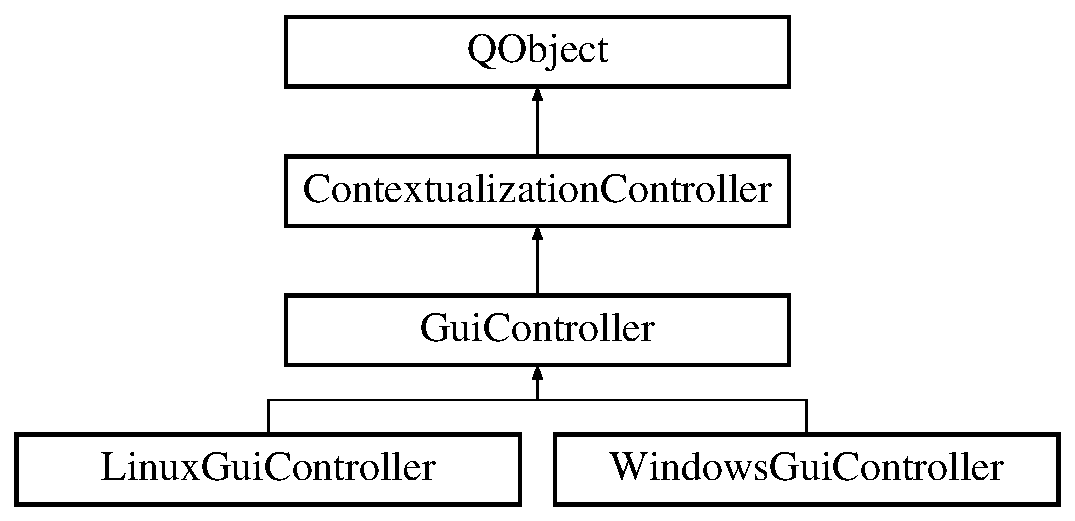
\includegraphics[height=4.000000cm]{classGuiController}
\end{center}
\end{figure}
\subsection*{Signals}
\begin{DoxyCompactItemize}
\item 
\mbox{\Hypertarget{classGuiController_a3bcaea6fb5694216afc69c4eca13b711}\label{classGuiController_a3bcaea6fb5694216afc69c4eca13b711}} 
void \mbox{\hyperlink{classGuiController_a3bcaea6fb5694216afc69c4eca13b711}{view\+Changed}} ()
\begin{DoxyCompactList}\small\item\em The singal is emitted when the pointer to the view changed. \end{DoxyCompactList}\item 
\mbox{\Hypertarget{classGuiController_a916ef2ef2d8d7b9ac4e63ee746dcdaaa}\label{classGuiController_a916ef2ef2d8d7b9ac4e63ee746dcdaaa}} 
void \mbox{\hyperlink{classGuiController_a916ef2ef2d8d7b9ac4e63ee746dcdaaa}{unchanged\+Project}} ()
\begin{DoxyCompactList}\small\item\em The signal is emitted when a current project is saved. \end{DoxyCompactList}\item 
\mbox{\Hypertarget{classGuiController_a20613f0b5eb1d49e4006a82ca80f17c5}\label{classGuiController_a20613f0b5eb1d49e4006a82ca80f17c5}} 
void \mbox{\hyperlink{classGuiController_a20613f0b5eb1d49e4006a82ca80f17c5}{strings\+List\+Changed}} ()
\begin{DoxyCompactList}\small\item\em The signal is emitted when a new string is added to the model or a string is removed from the model. \end{DoxyCompactList}\item 
\mbox{\Hypertarget{classGuiController_a8e5b5cd2b34a4c86d2b95acd1359b86a}\label{classGuiController_a8e5b5cd2b34a4c86d2b95acd1359b86a}} 
void \mbox{\hyperlink{classGuiController_a8e5b5cd2b34a4c86d2b95acd1359b86a}{image\+Changed}} ()
\begin{DoxyCompactList}\small\item\em The signal is emitted when a image is setted on the model. \end{DoxyCompactList}\end{DoxyCompactItemize}
\subsection*{Public Member Functions}
\begin{DoxyCompactItemize}
\item 
\mbox{\hyperlink{classGuiController_a853ee45214496ae1e59cd0139ecd1552}{Gui\+Controller}} (Q\+Quick\+Window $\ast$view=Q\+\_\+\+N\+U\+L\+L\+P\+TR, Q\+Object $\ast$parent=Q\+\_\+\+N\+U\+L\+L\+P\+TR)
\begin{DoxyCompactList}\small\item\em Creates an instance of a \mbox{\hyperlink{classGuiController}{Gui\+Controller}}. \end{DoxyCompactList}\item 
\mbox{\Hypertarget{classGuiController_a5b3332300c60a28c1f97a28ef51bac43}\label{classGuiController_a5b3332300c60a28c1f97a28ef51bac43}} 
\mbox{\hyperlink{classGuiController_a5b3332300c60a28c1f97a28ef51bac43}{$\sim$\+Gui\+Controller}} ()
\begin{DoxyCompactList}\small\item\em Destroys the \mbox{\hyperlink{classGuiController}{Gui\+Controller}}. \end{DoxyCompactList}\end{DoxyCompactItemize}
\subsection*{Properties}
\begin{DoxyCompactItemize}
\item 
\mbox{\Hypertarget{classGuiController_a10a671bf27008ab3e60e62b2106f8275}\label{classGuiController_a10a671bf27008ab3e60e62b2106f8275}} 
Q\+String {\bfseries image}
\item 
\mbox{\Hypertarget{classGuiController_a2ce97d522206f2adf3d38eb534f76d16}\label{classGuiController_a2ce97d522206f2adf3d38eb534f76d16}} 
Q\+List$<$ Q\+Object $\ast$ $>$ {\bfseries table\+Model}
\item 
\mbox{\Hypertarget{classGuiController_ad588a1633d6df3e17673232bc8a548dd}\label{classGuiController_ad588a1633d6df3e17673232bc8a548dd}} 
Q\+Quick\+Window {\bfseries view}
\item 
\mbox{\Hypertarget{classGuiController_a9130c47e3ab1205ed9c5a12a8afa9ec3}\label{classGuiController_a9130c47e3ab1205ed9c5a12a8afa9ec3}} 
bool {\bfseries only\+Done\+Strings}
\item 
\mbox{\Hypertarget{classGuiController_acf4e341b4f9b6c3c383c58531c494ecf}\label{classGuiController_acf4e341b4f9b6c3c383c58531c494ecf}} 
bool {\bfseries case\+Sensitive}
\end{DoxyCompactItemize}
\subsection*{Additional Inherited Members}


\subsection{Detailed Description}
This is the controller class that works a G\+UI environment. 

Definition at line 20 of file guicontroller.\+h.



\subsection{Constructor \& Destructor Documentation}
\mbox{\Hypertarget{classGuiController_a853ee45214496ae1e59cd0139ecd1552}\label{classGuiController_a853ee45214496ae1e59cd0139ecd1552}} 
\index{Gui\+Controller@{Gui\+Controller}!Gui\+Controller@{Gui\+Controller}}
\index{Gui\+Controller@{Gui\+Controller}!Gui\+Controller@{Gui\+Controller}}
\subsubsection{\texorpdfstring{Gui\+Controller()}{GuiController()}}
{\footnotesize\ttfamily Gui\+Controller\+::\+Gui\+Controller (\begin{DoxyParamCaption}\item[{Q\+Quick\+Window $\ast$}]{view = {\ttfamily Q\+\_\+NULLPTR},  }\item[{Q\+Object $\ast$}]{parent = {\ttfamily Q\+\_\+NULLPTR} }\end{DoxyParamCaption})}



Creates an instance of a \mbox{\hyperlink{classGuiController}{Gui\+Controller}}. 


\begin{DoxyParams}{Parameters}
{\em view} & Visual part of M\+VC. \\
\hline
{\em parent} & Parent object. \\
\hline
\end{DoxyParams}


Definition at line 13 of file guicontroller.\+cpp.



The documentation for this class was generated from the following files\+:\begin{DoxyCompactItemize}
\item 
src/contextualization/controller/\mbox{\hyperlink{guicontroller_8h}{guicontroller.\+h}}\item 
src/contextualization/controller/\mbox{\hyperlink{guicontroller_8cpp}{guicontroller.\+cpp}}\end{DoxyCompactItemize}

\hypertarget{classHpContextualizationFactory}{}\section{Hp\+Contextualization\+Factory Class Reference}
\label{classHpContextualizationFactory}\index{Hp\+Contextualization\+Factory@{Hp\+Contextualization\+Factory}}


This is a factory to create a concrete class of \mbox{\hyperlink{classContextualizationController}{Contextualization\+Controller}} specific for HP company.  




{\ttfamily \#include $<$hpcontextualizationfactory.\+h$>$}

Inheritance diagram for Hp\+Contextualization\+Factory\+:\begin{figure}[H]
\begin{center}
\leavevmode
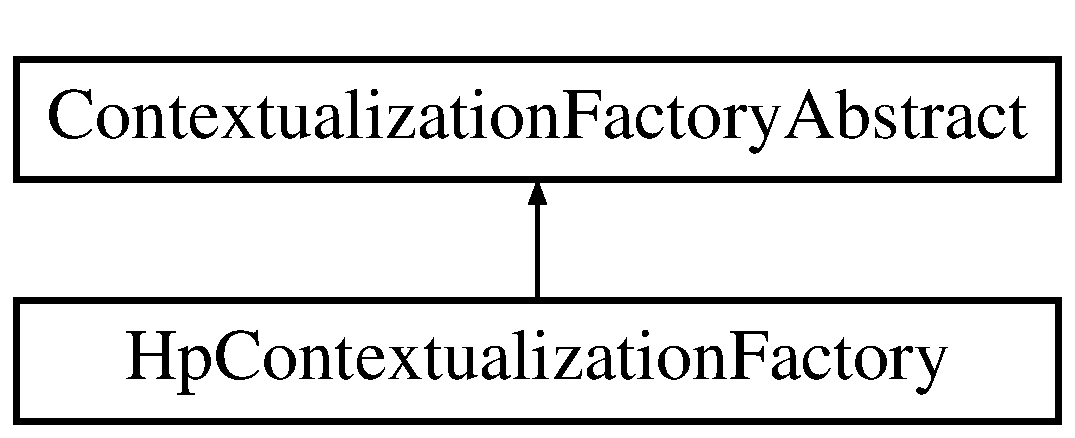
\includegraphics[height=2.000000cm]{classHpContextualizationFactory}
\end{center}
\end{figure}
\subsection*{Public Member Functions}
\begin{DoxyCompactItemize}
\item 
\mbox{\Hypertarget{classHpContextualizationFactory_afee11305ab5203745cddd4a837542ea3}\label{classHpContextualizationFactory_afee11305ab5203745cddd4a837542ea3}} 
\mbox{\hyperlink{classHpContextualizationFactory_afee11305ab5203745cddd4a837542ea3}{Hp\+Contextualization\+Factory}} ()
\begin{DoxyCompactList}\small\item\em Creates an empty \mbox{\hyperlink{classHpContextualizationFactory}{Hp\+Contextualization\+Factory}}. \end{DoxyCompactList}\item 
\mbox{\hyperlink{classContextualizationController}{Contextualization\+Controller}} $\ast$ \mbox{\hyperlink{classHpContextualizationFactory_ad9d9c11a2827c8854c4cadbf38b4e7ca}{create\+Controller}} (char $\ast$$\ast$params, int count) override
\begin{DoxyCompactList}\small\item\em Creates a new \mbox{\hyperlink{classContextualizationController}{Contextualization\+Controller}}. \end{DoxyCompactList}\end{DoxyCompactItemize}
\subsection*{Additional Inherited Members}


\subsection{Detailed Description}
This is a factory to create a concrete class of \mbox{\hyperlink{classContextualizationController}{Contextualization\+Controller}} specific for HP company. 

Definition at line 21 of file hpcontextualizationfactory.\+h.



\subsection{Member Function Documentation}
\mbox{\Hypertarget{classHpContextualizationFactory_ad9d9c11a2827c8854c4cadbf38b4e7ca}\label{classHpContextualizationFactory_ad9d9c11a2827c8854c4cadbf38b4e7ca}} 
\index{Hp\+Contextualization\+Factory@{Hp\+Contextualization\+Factory}!create\+Controller@{create\+Controller}}
\index{create\+Controller@{create\+Controller}!Hp\+Contextualization\+Factory@{Hp\+Contextualization\+Factory}}
\subsubsection{\texorpdfstring{create\+Controller()}{createController()}}
{\footnotesize\ttfamily \mbox{\hyperlink{classContextualizationController}{Contextualization\+Controller}} $\ast$ Hp\+Contextualization\+Factory\+::create\+Controller (\begin{DoxyParamCaption}\item[{char $\ast$$\ast$}]{params,  }\item[{int}]{count }\end{DoxyParamCaption})\hspace{0.3cm}{\ttfamily [override]}, {\ttfamily [virtual]}}



Creates a new \mbox{\hyperlink{classContextualizationController}{Contextualization\+Controller}}. 

Creates one type of \mbox{\hyperlink{classContextualizationController}{Contextualization\+Controller}} depending of received params and the operate system where de application is running. 
\begin{DoxyParams}{Parameters}
{\em params} & Array params. \\
\hline
{\em count} & Number of elements of params array. \\
\hline
\end{DoxyParams}
\begin{DoxyReturn}{Returns}
Contextualization pointer. 
\end{DoxyReturn}


Implements \mbox{\hyperlink{classContextualizationFactoryAbstract_a0898ad4d3a109c5767a1e596bf444e4a}{Contextualization\+Factory\+Abstract}}.



Definition at line 18 of file hpcontextualizationfactory.\+cpp.



The documentation for this class was generated from the following files\+:\begin{DoxyCompactItemize}
\item 
src/tools/\mbox{\hyperlink{hpcontextualizationfactory_8h}{hpcontextualizationfactory.\+h}}\item 
src/tools/\mbox{\hyperlink{hpcontextualizationfactory_8cpp}{hpcontextualizationfactory.\+cpp}}\end{DoxyCompactItemize}

\hypertarget{classLinuxConsoleController}{}\section{Linux\+Console\+Controller Class Reference}
\label{classLinuxConsoleController}\index{Linux\+Console\+Controller@{Linux\+Console\+Controller}}


This is the controller class that works a linux C\+LI environment.  




{\ttfamily \#include $<$linuxconsolecontroller.\+h$>$}

Inheritance diagram for Linux\+Console\+Controller\+:\begin{figure}[H]
\begin{center}
\leavevmode
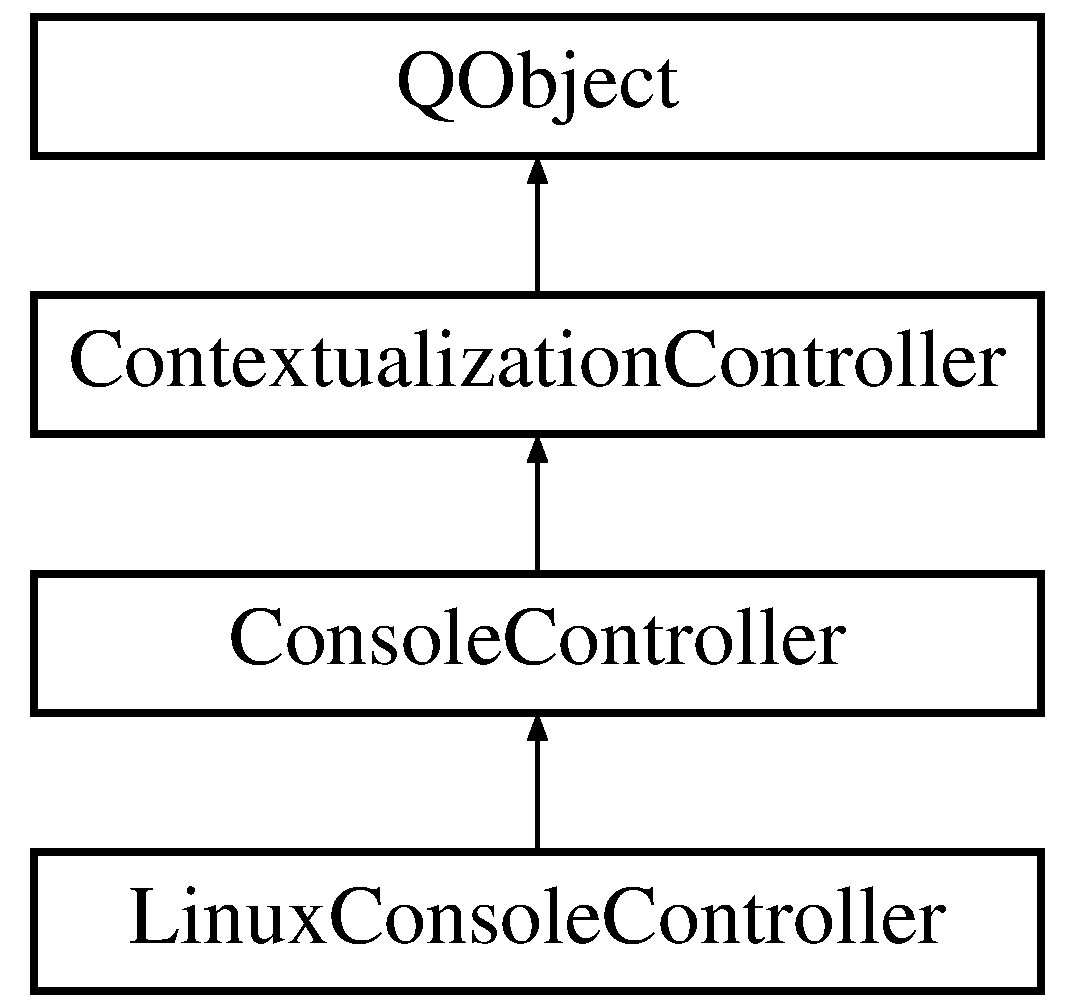
\includegraphics[height=4.000000cm]{classLinuxConsoleController}
\end{center}
\end{figure}
\subsection*{Public Member Functions}
\begin{DoxyCompactItemize}
\item 
\mbox{\Hypertarget{classLinuxConsoleController_a22dbaf4b36c07b2bc729287c93118853}\label{classLinuxConsoleController_a22dbaf4b36c07b2bc729287c93118853}} 
\mbox{\hyperlink{classLinuxConsoleController_a22dbaf4b36c07b2bc729287c93118853}{Linux\+Console\+Controller}} ()
\begin{DoxyCompactList}\small\item\em Creates an empty \mbox{\hyperlink{classLinuxConsoleController}{Linux\+Console\+Controller}}. \end{DoxyCompactList}\item 
\mbox{\hyperlink{classLinuxConsoleController_a28e3374d97058fa2649d2582686bfe6f}{Linux\+Console\+Controller}} (int argc, char $\ast$$\ast$argv)
\begin{DoxyCompactList}\small\item\em Creates a \mbox{\hyperlink{classLinuxConsoleController}{Linux\+Console\+Controller}} initialited with the parameter received in argv. \end{DoxyCompactList}\item 
Q\+String \mbox{\hyperlink{classLinuxConsoleController_ac9944bf1302b077c733802349359e777}{take\+Capture\+Area}} () override
\begin{DoxyCompactList}\small\item\em Starts a process that allow user capture an area of the screen. \end{DoxyCompactList}\end{DoxyCompactItemize}
\subsection*{Additional Inherited Members}


\subsection{Detailed Description}
This is the controller class that works a linux C\+LI environment. 

Definition at line 17 of file linuxconsolecontroller.\+h.



\subsection{Constructor \& Destructor Documentation}
\mbox{\Hypertarget{classLinuxConsoleController_a28e3374d97058fa2649d2582686bfe6f}\label{classLinuxConsoleController_a28e3374d97058fa2649d2582686bfe6f}} 
\index{Linux\+Console\+Controller@{Linux\+Console\+Controller}!Linux\+Console\+Controller@{Linux\+Console\+Controller}}
\index{Linux\+Console\+Controller@{Linux\+Console\+Controller}!Linux\+Console\+Controller@{Linux\+Console\+Controller}}
\subsubsection{\texorpdfstring{Linux\+Console\+Controller()}{LinuxConsoleController()}}
{\footnotesize\ttfamily Linux\+Console\+Controller\+::\+Linux\+Console\+Controller (\begin{DoxyParamCaption}\item[{int}]{argc,  }\item[{char $\ast$$\ast$}]{argv }\end{DoxyParamCaption})}



Creates a \mbox{\hyperlink{classLinuxConsoleController}{Linux\+Console\+Controller}} initialited with the parameter received in argv. 


\begin{DoxyParams}{Parameters}
{\em argc} & Number of elements of argv. \\
\hline
{\em argv} & Parameters \\
\hline
\end{DoxyParams}


Definition at line 18 of file linuxconsolecontroller.\+cpp.



\subsection{Member Function Documentation}
\mbox{\Hypertarget{classLinuxConsoleController_ac9944bf1302b077c733802349359e777}\label{classLinuxConsoleController_ac9944bf1302b077c733802349359e777}} 
\index{Linux\+Console\+Controller@{Linux\+Console\+Controller}!take\+Capture\+Area@{take\+Capture\+Area}}
\index{take\+Capture\+Area@{take\+Capture\+Area}!Linux\+Console\+Controller@{Linux\+Console\+Controller}}
\subsubsection{\texorpdfstring{take\+Capture\+Area()}{takeCaptureArea()}}
{\footnotesize\ttfamily Q\+String Linux\+Console\+Controller\+::take\+Capture\+Area (\begin{DoxyParamCaption}{ }\end{DoxyParamCaption})\hspace{0.3cm}{\ttfamily [override]}, {\ttfamily [virtual]}}



Starts a process that allow user capture an area of the screen. 

The user have to select the area to capture with the mouse. Return the path where the capture is stored or an empty Q\+String if an error ocurred. \begin{DoxyReturn}{Returns}
Q\+String 
\end{DoxyReturn}


Implements \mbox{\hyperlink{classContextualizationController_a121919886590cd4955bbcc2d8b747b26}{Contextualization\+Controller}}.



Definition at line 23 of file linuxconsolecontroller.\+cpp.



The documentation for this class was generated from the following files\+:\begin{DoxyCompactItemize}
\item 
src/contextualization/controller/\mbox{\hyperlink{linuxconsolecontroller_8h}{linuxconsolecontroller.\+h}}\item 
src/contextualization/controller/\mbox{\hyperlink{linuxconsolecontroller_8cpp}{linuxconsolecontroller.\+cpp}}\end{DoxyCompactItemize}

\hypertarget{classLinuxGuiController}{}\section{Linux\+Gui\+Controller Class Reference}
\label{classLinuxGuiController}\index{Linux\+Gui\+Controller@{Linux\+Gui\+Controller}}


This is the controller class that works a linux G\+UI environment.  




{\ttfamily \#include $<$linuxguicontroller.\+h$>$}

Inheritance diagram for Linux\+Gui\+Controller\+:\begin{figure}[H]
\begin{center}
\leavevmode
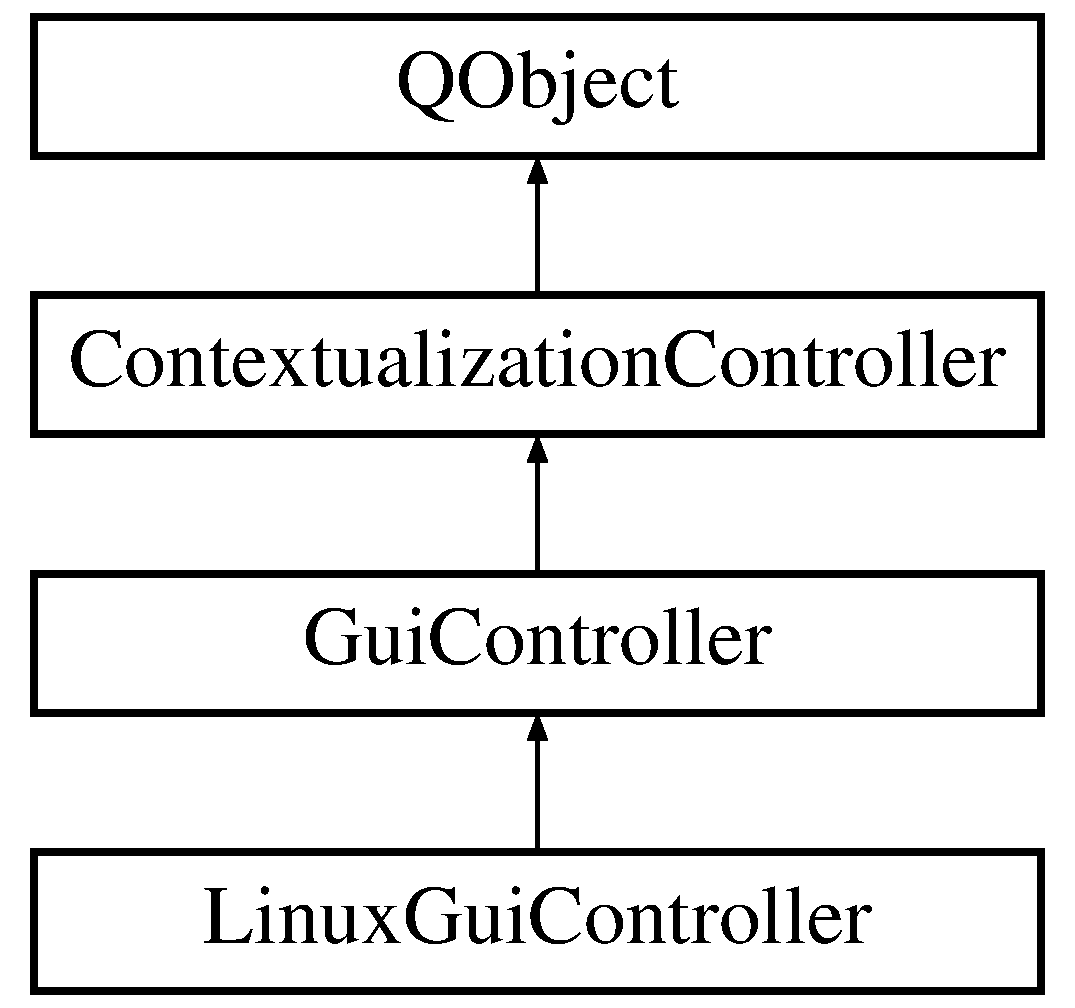
\includegraphics[height=4.000000cm]{classLinuxGuiController}
\end{center}
\end{figure}
\subsection*{Public Member Functions}
\begin{DoxyCompactItemize}
\item 
\mbox{\hyperlink{classLinuxGuiController_a26b28a0d7854973830048c9087a3cdf1}{Linux\+Gui\+Controller}} (Q\+Quick\+Window $\ast$view=Q\+\_\+\+N\+U\+L\+L\+P\+TR, Q\+Object $\ast$parent=Q\+\_\+\+N\+U\+L\+L\+P\+TR)
\begin{DoxyCompactList}\small\item\em \mbox{\hyperlink{classLinuxGuiController}{Linux\+Gui\+Controller}}. \end{DoxyCompactList}\item 
Q\+String \mbox{\hyperlink{classLinuxGuiController_a8242963a9c5f4b967902f8ee576294ec}{take\+Capture\+Area}} () override
\begin{DoxyCompactList}\small\item\em Starts a process that allow user capture an area of the screen. \end{DoxyCompactList}\end{DoxyCompactItemize}
\subsection*{Additional Inherited Members}


\subsection{Detailed Description}
This is the controller class that works a linux G\+UI environment. 

Definition at line 16 of file linuxguicontroller.\+h.



\subsection{Constructor \& Destructor Documentation}
\mbox{\Hypertarget{classLinuxGuiController_a26b28a0d7854973830048c9087a3cdf1}\label{classLinuxGuiController_a26b28a0d7854973830048c9087a3cdf1}} 
\index{Linux\+Gui\+Controller@{Linux\+Gui\+Controller}!Linux\+Gui\+Controller@{Linux\+Gui\+Controller}}
\index{Linux\+Gui\+Controller@{Linux\+Gui\+Controller}!Linux\+Gui\+Controller@{Linux\+Gui\+Controller}}
\subsubsection{\texorpdfstring{Linux\+Gui\+Controller()}{LinuxGuiController()}}
{\footnotesize\ttfamily Linux\+Gui\+Controller\+::\+Linux\+Gui\+Controller (\begin{DoxyParamCaption}\item[{Q\+Quick\+Window $\ast$}]{view = {\ttfamily Q\+\_\+NULLPTR},  }\item[{Q\+Object $\ast$}]{parent = {\ttfamily Q\+\_\+NULLPTR} }\end{DoxyParamCaption})}



\mbox{\hyperlink{classLinuxGuiController}{Linux\+Gui\+Controller}}. 


\begin{DoxyParams}{Parameters}
{\em view} & \\
\hline
{\em parent} & \\
\hline
\end{DoxyParams}


Definition at line 13 of file linuxguicontroller.\+cpp.



\subsection{Member Function Documentation}
\mbox{\Hypertarget{classLinuxGuiController_a8242963a9c5f4b967902f8ee576294ec}\label{classLinuxGuiController_a8242963a9c5f4b967902f8ee576294ec}} 
\index{Linux\+Gui\+Controller@{Linux\+Gui\+Controller}!take\+Capture\+Area@{take\+Capture\+Area}}
\index{take\+Capture\+Area@{take\+Capture\+Area}!Linux\+Gui\+Controller@{Linux\+Gui\+Controller}}
\subsubsection{\texorpdfstring{take\+Capture\+Area()}{takeCaptureArea()}}
{\footnotesize\ttfamily Q\+String Linux\+Gui\+Controller\+::take\+Capture\+Area (\begin{DoxyParamCaption}{ }\end{DoxyParamCaption})\hspace{0.3cm}{\ttfamily [override]}, {\ttfamily [virtual]}}



Starts a process that allow user capture an area of the screen. 

The user have to select the area to capture with the mouse. Return the path where the capture is stored or an empty Q\+String if an error ocurred. \begin{DoxyReturn}{Returns}
Q\+String 
\end{DoxyReturn}


Implements \mbox{\hyperlink{classContextualizationController_a121919886590cd4955bbcc2d8b747b26}{Contextualization\+Controller}}.



Definition at line 18 of file linuxguicontroller.\+cpp.



The documentation for this class was generated from the following files\+:\begin{DoxyCompactItemize}
\item 
src/contextualization/controller/\mbox{\hyperlink{linuxguicontroller_8h}{linuxguicontroller.\+h}}\item 
src/contextualization/controller/\mbox{\hyperlink{linuxguicontroller_8cpp}{linuxguicontroller.\+cpp}}\end{DoxyCompactItemize}

\hypertarget{classLog}{}\section{Log Class Reference}
\label{classLog}\index{Log@{Log}}


This is a static class to write logs in different channels.  




{\ttfamily \#include $<$log.\+h$>$}

\subsection*{Public Member Functions}
\begin{DoxyCompactItemize}
\item 
\mbox{\Hypertarget{classLog_af6071a60aa52b6c1b511f99b4bc1b8fe}\label{classLog_af6071a60aa52b6c1b511f99b4bc1b8fe}} 
\mbox{\hyperlink{classLog_af6071a60aa52b6c1b511f99b4bc1b8fe}{Log}} ()
\begin{DoxyCompactList}\small\item\em Constructs an empty log. Doesn\textquotesingle{}t do anything. \end{DoxyCompactList}\end{DoxyCompactItemize}
\subsection*{Static Public Member Functions}
\begin{DoxyCompactItemize}
\item 
static void \mbox{\hyperlink{classLog_a8291d71e5438b70ac71232a23606690a}{write\+Debug}} (Q\+String text)
\begin{DoxyCompactList}\small\item\em Appends a debug mensage containig text received by parameter in the debug file. \end{DoxyCompactList}\item 
static void \mbox{\hyperlink{classLog_a1808c128874dd41cca3536ed5672df12}{write\+Log}} (Q\+String text)
\begin{DoxyCompactList}\small\item\em Appends a log mensage containig text received by parameter in the log file. \end{DoxyCompactList}\item 
static void \mbox{\hyperlink{classLog_ae35819424f49efa88b29a0bccc962f93}{write\+Error}} (Q\+String text)
\begin{DoxyCompactList}\small\item\em Appends an error mensage containig text received by parameter in the error file. \end{DoxyCompactList}\end{DoxyCompactItemize}


\subsection{Detailed Description}
This is a static class to write logs in different channels. 

Definition at line 27 of file log.\+h.



\subsection{Member Function Documentation}
\mbox{\Hypertarget{classLog_a8291d71e5438b70ac71232a23606690a}\label{classLog_a8291d71e5438b70ac71232a23606690a}} 
\index{Log@{Log}!write\+Debug@{write\+Debug}}
\index{write\+Debug@{write\+Debug}!Log@{Log}}
\subsubsection{\texorpdfstring{write\+Debug()}{writeDebug()}}
{\footnotesize\ttfamily void Log\+::write\+Debug (\begin{DoxyParamCaption}\item[{Q\+String}]{text }\end{DoxyParamCaption})\hspace{0.3cm}{\ttfamily [static]}}



Appends a debug mensage containig text received by parameter in the debug file. 


\begin{DoxyParams}{Parameters}
{\em text} & Text to write in file. \\
\hline
\end{DoxyParams}


Definition at line 25 of file log.\+cpp.

\mbox{\Hypertarget{classLog_ae35819424f49efa88b29a0bccc962f93}\label{classLog_ae35819424f49efa88b29a0bccc962f93}} 
\index{Log@{Log}!write\+Error@{write\+Error}}
\index{write\+Error@{write\+Error}!Log@{Log}}
\subsubsection{\texorpdfstring{write\+Error()}{writeError()}}
{\footnotesize\ttfamily void Log\+::write\+Error (\begin{DoxyParamCaption}\item[{Q\+String}]{text }\end{DoxyParamCaption})\hspace{0.3cm}{\ttfamily [static]}}



Appends an error mensage containig text received by parameter in the error file. 


\begin{DoxyParams}{Parameters}
{\em text} & Text to write in file. \\
\hline
\end{DoxyParams}


Definition at line 42 of file log.\+cpp.

\mbox{\Hypertarget{classLog_a1808c128874dd41cca3536ed5672df12}\label{classLog_a1808c128874dd41cca3536ed5672df12}} 
\index{Log@{Log}!write\+Log@{write\+Log}}
\index{write\+Log@{write\+Log}!Log@{Log}}
\subsubsection{\texorpdfstring{write\+Log()}{writeLog()}}
{\footnotesize\ttfamily void Log\+::write\+Log (\begin{DoxyParamCaption}\item[{Q\+String}]{text }\end{DoxyParamCaption})\hspace{0.3cm}{\ttfamily [static]}}



Appends a log mensage containig text received by parameter in the log file. 


\begin{DoxyParams}{Parameters}
{\em text} & Text to write in file. \\
\hline
\end{DoxyParams}


Definition at line 34 of file log.\+cpp.



The documentation for this class was generated from the following files\+:\begin{DoxyCompactItemize}
\item 
src/tools/\mbox{\hyperlink{log_8h}{log.\+h}}\item 
src/tools/\mbox{\hyperlink{log_8cpp}{log.\+cpp}}\end{DoxyCompactItemize}

\hypertarget{classMySqlConnector}{}\section{My\+Sql\+Connector Class Reference}
\label{classMySqlConnector}\index{My\+Sql\+Connector@{My\+Sql\+Connector}}


This is a class to access a My\+S\+QL database.  




{\ttfamily \#include $<$mysqlconnector.\+h$>$}

Inheritance diagram for My\+Sql\+Connector\+:\begin{figure}[H]
\begin{center}
\leavevmode
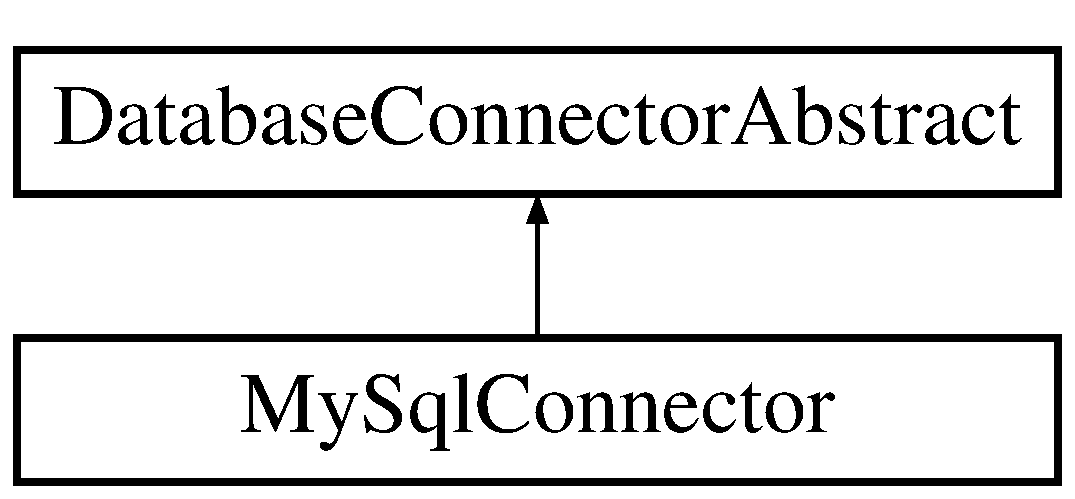
\includegraphics[height=2.000000cm]{classMySqlConnector}
\end{center}
\end{figure}
\subsection*{Public Member Functions}
\begin{DoxyCompactItemize}
\item 
\mbox{\Hypertarget{classMySqlConnector_af17a58a3749687938d0b3b15e276dab7}\label{classMySqlConnector_af17a58a3749687938d0b3b15e276dab7}} 
\mbox{\hyperlink{classMySqlConnector_af17a58a3749687938d0b3b15e276dab7}{My\+Sql\+Connector}} ()
\begin{DoxyCompactList}\small\item\em Creates an empty \mbox{\hyperlink{classMySqlConnector}{My\+Sql\+Connector}}. \end{DoxyCompactList}\item 
\mbox{\hyperlink{classMySqlConnector_a86344c8e5fb792da1da746bdea3a2474}{My\+Sql\+Connector}} (const Q\+String host, const Q\+String user, const Q\+String password, const Q\+String database=Q\+String())
\begin{DoxyCompactList}\small\item\em Creates a \mbox{\hyperlink{classMySqlConnector}{My\+Sql\+Connector}} setting values received by argument. \end{DoxyCompactList}\item 
Q\+String \mbox{\hyperlink{classMySqlConnector_ae652c2a79321d979121e2347cbb25ba0}{get\+User}} ()
\begin{DoxyCompactList}\small\item\em Returns a user name to access database. \end{DoxyCompactList}\item 
void \mbox{\hyperlink{classMySqlConnector_a0cf4bedae2d4093449590aa59d200ce8}{set\+User}} (const Q\+String user)
\begin{DoxyCompactList}\small\item\em Sets username to access database. \end{DoxyCompactList}\item 
void \mbox{\hyperlink{classMySqlConnector_a92af1c28da0953a69573b21f68b8a41f}{set\+Password}} (const Q\+String password)
\begin{DoxyCompactList}\small\item\em Sets password to access database. \end{DoxyCompactList}\item 
Q\+String \mbox{\hyperlink{classMySqlConnector_a9bada8a552b17c5e39e7d1c903201b4b}{get\+Data\+Base}} ()
\begin{DoxyCompactList}\small\item\em Returns a data base name to access database. \end{DoxyCompactList}\item 
void \mbox{\hyperlink{classMySqlConnector_a8688bfeb3bb6ba6181f5ce90dc8066d8}{set\+Data\+Base}} (const Q\+String data\+Base)
\begin{DoxyCompactList}\small\item\em Sets data base to access database. \end{DoxyCompactList}\item 
Q\+List$<$ \mbox{\hyperlink{classString}{String}} $\ast$ $>$ \mbox{\hyperlink{classMySqlConnector_ad6ff79c4049e3631800da97e8d7b7704}{get\+All\+Strings}} () override
\item 
Q\+List$<$ \mbox{\hyperlink{classString}{String}} $\ast$ $>$ \mbox{\hyperlink{classMySqlConnector_ae7440816a5bda9e63ea526656c4001f5}{get\+Strings\+With\+Value}} (const Q\+String \&value, bool case\+Sensitive=true) override
\begin{DoxyCompactList}\small\item\em Returns all strigns in database with the value received by argument. \end{DoxyCompactList}\item 
Q\+List$<$ \mbox{\hyperlink{classString}{String}} $\ast$ $>$ \mbox{\hyperlink{classMySqlConnector_a8a480141c72dc8da687b15f921ab1a4e}{get\+Strings\+With\+Approximate\+Value}} (const Q\+String \&value, bool case\+Sensitive=true) override
\begin{DoxyCompactList}\small\item\em Returns all strigns in database with a similar value received by argument. \end{DoxyCompactList}\item 
Q\+List$<$ \mbox{\hyperlink{classString}{String}} $\ast$ $>$ \mbox{\hyperlink{classMySqlConnector_a269bbced50451ff0ce48cfc4f2bb6a3b}{get\+String\+With\+Id}} (const Q\+String \&id, bool case\+Sensitive=true) override
\begin{DoxyCompactList}\small\item\em Returns all strigns in database with the identifier received by argument. \end{DoxyCompactList}\item 
Q\+List$<$ \mbox{\hyperlink{classString}{String}} $\ast$ $>$ \mbox{\hyperlink{classMySqlConnector_a821c3dcebcd763df1700881cb47685d5}{get\+Strings\+With\+State}} (const Q\+String state) override
\begin{DoxyCompactList}\small\item\em Returns strings with state received by parameter. \end{DoxyCompactList}\item 
bool \mbox{\hyperlink{classMySqlConnector_a4608c0764241969454a55b42873cb86b}{insert\+String}} (const \mbox{\hyperlink{classString}{String}} \&string, const Q\+String language) override
\begin{DoxyCompactList}\small\item\em Inserts a new string in database. \end{DoxyCompactList}\item 
int \mbox{\hyperlink{classMySqlConnector_a77a5169dd8a515b613642c88dac9798b}{insert\+Strings}} (const Q\+List$<$ \mbox{\hyperlink{classString}{String}} $\ast$$>$ \&strings, const Q\+String language) override
\begin{DoxyCompactList}\small\item\em Inserts a set of strings into the database. \end{DoxyCompactList}\item 
int \mbox{\hyperlink{classMySqlConnector_a528aac591ea56ade27a096bb997abb2a}{remove\+Strings\+With\+Value}} (const Q\+String \&value, bool case\+Sensitive=true) override
\begin{DoxyCompactList}\small\item\em Removes from databse all strigns with the value received by argument. \end{DoxyCompactList}\item 
int \mbox{\hyperlink{classMySqlConnector_a3c340e5310c56410d64ecd89e5cf6661}{remove\+Strings\+With\+Id}} (const Q\+String \&id, bool case\+Sensitive=true) override
\begin{DoxyCompactList}\small\item\em Removes from databse the strign with the identifier received by argument. \end{DoxyCompactList}\item 
Q\+String\+List \mbox{\hyperlink{classMySqlConnector_a83be1a4d67e509b6604629660eb7c4a0}{get\+Languages}} () override
\begin{DoxyCompactList}\small\item\em Returns all languages stored in database. \end{DoxyCompactList}\item 
Q\+String\+List \mbox{\hyperlink{classMySqlConnector_a3493828360c7edd217461e040fc1b00e}{get\+Language\+Ids}} () override
\begin{DoxyCompactList}\small\item\em Returns all language identifiers stored in database. \end{DoxyCompactList}\item 
Q\+String \mbox{\hyperlink{classMySqlConnector_a16a6f0883e2b384621e738f78c619af6}{get\+Key\+From\+Language}} (const Q\+String language)
\begin{DoxyCompactList}\small\item\em Returns the key of language received by parameter. \end{DoxyCompactList}\end{DoxyCompactItemize}
\subsection*{Additional Inherited Members}


\subsection{Detailed Description}
This is a class to access a My\+S\+QL database. 

Definition at line 20 of file mysqlconnector.\+h.



\subsection{Constructor \& Destructor Documentation}
\mbox{\Hypertarget{classMySqlConnector_a86344c8e5fb792da1da746bdea3a2474}\label{classMySqlConnector_a86344c8e5fb792da1da746bdea3a2474}} 
\index{My\+Sql\+Connector@{My\+Sql\+Connector}!My\+Sql\+Connector@{My\+Sql\+Connector}}
\index{My\+Sql\+Connector@{My\+Sql\+Connector}!My\+Sql\+Connector@{My\+Sql\+Connector}}
\subsubsection{\texorpdfstring{My\+Sql\+Connector()}{MySqlConnector()}}
{\footnotesize\ttfamily My\+Sql\+Connector\+::\+My\+Sql\+Connector (\begin{DoxyParamCaption}\item[{const Q\+String}]{host,  }\item[{const Q\+String}]{user,  }\item[{const Q\+String}]{password,  }\item[{const Q\+String}]{database = {\ttfamily QString()} }\end{DoxyParamCaption})}



Creates a \mbox{\hyperlink{classMySqlConnector}{My\+Sql\+Connector}} setting values received by argument. 


\begin{DoxyParams}{Parameters}
{\em user} & Username to access database. \\
\hline
{\em password} & Password for the username. \\
\hline
{\em database} & Data base name. \\
\hline
{\em table} & Table name. \\
\hline
\end{DoxyParams}


Definition at line 13 of file mysqlconnector.\+cpp.



\subsection{Member Function Documentation}
\mbox{\Hypertarget{classMySqlConnector_ad6ff79c4049e3631800da97e8d7b7704}\label{classMySqlConnector_ad6ff79c4049e3631800da97e8d7b7704}} 
\index{My\+Sql\+Connector@{My\+Sql\+Connector}!get\+All\+Strings@{get\+All\+Strings}}
\index{get\+All\+Strings@{get\+All\+Strings}!My\+Sql\+Connector@{My\+Sql\+Connector}}
\subsubsection{\texorpdfstring{get\+All\+Strings()}{getAllStrings()}}
{\footnotesize\ttfamily Q\+List$<$ \mbox{\hyperlink{classString}{String}} $\ast$ $>$ My\+Sql\+Connector\+::get\+All\+Strings (\begin{DoxyParamCaption}{ }\end{DoxyParamCaption})\hspace{0.3cm}{\ttfamily [override]}, {\ttfamily [virtual]}}







Implements \mbox{\hyperlink{classDatabaseConnectorAbstract_aeb4347bc18b6bed9a9b6120f68c10e9d}{Database\+Connector\+Abstract}}.



Definition at line 64 of file mysqlconnector.\+cpp.

\mbox{\Hypertarget{classMySqlConnector_a9bada8a552b17c5e39e7d1c903201b4b}\label{classMySqlConnector_a9bada8a552b17c5e39e7d1c903201b4b}} 
\index{My\+Sql\+Connector@{My\+Sql\+Connector}!get\+Data\+Base@{get\+Data\+Base}}
\index{get\+Data\+Base@{get\+Data\+Base}!My\+Sql\+Connector@{My\+Sql\+Connector}}
\subsubsection{\texorpdfstring{get\+Data\+Base()}{getDataBase()}}
{\footnotesize\ttfamily Q\+String My\+Sql\+Connector\+::get\+Data\+Base (\begin{DoxyParamCaption}{ }\end{DoxyParamCaption})}



Returns a data base name to access database. 

\begin{DoxyReturn}{Returns}
User name. 
\end{DoxyReturn}


Definition at line 54 of file mysqlconnector.\+cpp.

\mbox{\Hypertarget{classMySqlConnector_a16a6f0883e2b384621e738f78c619af6}\label{classMySqlConnector_a16a6f0883e2b384621e738f78c619af6}} 
\index{My\+Sql\+Connector@{My\+Sql\+Connector}!get\+Key\+From\+Language@{get\+Key\+From\+Language}}
\index{get\+Key\+From\+Language@{get\+Key\+From\+Language}!My\+Sql\+Connector@{My\+Sql\+Connector}}
\subsubsection{\texorpdfstring{get\+Key\+From\+Language()}{getKeyFromLanguage()}}
{\footnotesize\ttfamily Q\+String My\+Sql\+Connector\+::get\+Key\+From\+Language (\begin{DoxyParamCaption}\item[{const Q\+String}]{language }\end{DoxyParamCaption})}



Returns the key of language received by parameter. 


\begin{DoxyParams}{Parameters}
{\em language} & Language to match key \\
\hline
\end{DoxyParams}
\begin{DoxyReturn}{Returns}
Language ID 
\end{DoxyReturn}


Definition at line 326 of file mysqlconnector.\+cpp.

\mbox{\Hypertarget{classMySqlConnector_a3493828360c7edd217461e040fc1b00e}\label{classMySqlConnector_a3493828360c7edd217461e040fc1b00e}} 
\index{My\+Sql\+Connector@{My\+Sql\+Connector}!get\+Language\+Ids@{get\+Language\+Ids}}
\index{get\+Language\+Ids@{get\+Language\+Ids}!My\+Sql\+Connector@{My\+Sql\+Connector}}
\subsubsection{\texorpdfstring{get\+Language\+Ids()}{getLanguageIds()}}
{\footnotesize\ttfamily Q\+String\+List My\+Sql\+Connector\+::get\+Language\+Ids (\begin{DoxyParamCaption}{ }\end{DoxyParamCaption})\hspace{0.3cm}{\ttfamily [override]}, {\ttfamily [virtual]}}



Returns all language identifiers stored in database. 

\begin{DoxyReturn}{Returns}
Languages used. 
\end{DoxyReturn}


Implements \mbox{\hyperlink{classDatabaseConnectorAbstract_a98f5b2472bab6edc82ce2c5554319d7f}{Database\+Connector\+Abstract}}.



Definition at line 308 of file mysqlconnector.\+cpp.

\mbox{\Hypertarget{classMySqlConnector_a83be1a4d67e509b6604629660eb7c4a0}\label{classMySqlConnector_a83be1a4d67e509b6604629660eb7c4a0}} 
\index{My\+Sql\+Connector@{My\+Sql\+Connector}!get\+Languages@{get\+Languages}}
\index{get\+Languages@{get\+Languages}!My\+Sql\+Connector@{My\+Sql\+Connector}}
\subsubsection{\texorpdfstring{get\+Languages()}{getLanguages()}}
{\footnotesize\ttfamily Q\+String\+List My\+Sql\+Connector\+::get\+Languages (\begin{DoxyParamCaption}{ }\end{DoxyParamCaption})\hspace{0.3cm}{\ttfamily [override]}, {\ttfamily [virtual]}}



Returns all languages stored in database. 

\begin{DoxyReturn}{Returns}
Languages used. 
\end{DoxyReturn}


Implements \mbox{\hyperlink{classDatabaseConnectorAbstract_a77ff263d407366e54f3e8512c575ff5e}{Database\+Connector\+Abstract}}.



Definition at line 290 of file mysqlconnector.\+cpp.

\mbox{\Hypertarget{classMySqlConnector_a8a480141c72dc8da687b15f921ab1a4e}\label{classMySqlConnector_a8a480141c72dc8da687b15f921ab1a4e}} 
\index{My\+Sql\+Connector@{My\+Sql\+Connector}!get\+Strings\+With\+Approximate\+Value@{get\+Strings\+With\+Approximate\+Value}}
\index{get\+Strings\+With\+Approximate\+Value@{get\+Strings\+With\+Approximate\+Value}!My\+Sql\+Connector@{My\+Sql\+Connector}}
\subsubsection{\texorpdfstring{get\+Strings\+With\+Approximate\+Value()}{getStringsWithApproximateValue()}}
{\footnotesize\ttfamily Q\+List$<$ \mbox{\hyperlink{classString}{String}} $\ast$ $>$ My\+Sql\+Connector\+::get\+Strings\+With\+Approximate\+Value (\begin{DoxyParamCaption}\item[{const Q\+String \&}]{value,  }\item[{bool}]{case\+Sensitive = {\ttfamily true} }\end{DoxyParamCaption})\hspace{0.3cm}{\ttfamily [override]}, {\ttfamily [virtual]}}



Returns all strigns in database with a similar value received by argument. 


\begin{DoxyParams}{Parameters}
{\em value} & \mbox{\hyperlink{classString}{String}} value. \\
\hline
\end{DoxyParams}
\begin{DoxyReturn}{Returns}
List with strings. 
\end{DoxyReturn}
If the value belongs to a string, the fw\+String is saved, otherwise relsease memory of fw\+String. If size of both strings is longer than M\+I\+N\+\_\+\+L\+E\+N\+G\+T\+H\+\_\+\+F\+O\+R\+\_\+\+A\+P\+P\+R\+O\+X\+I\+M\+A\+TE and their size difference is less than M\+A\+X\+\_\+\+L\+E\+N\+G\+T\+H\+\_\+\+D\+I\+F\+F\+E\+R\+E\+N\+CE, a value is considered valid if it is contained within the fw\+String value or vice versa. If size of any strings is less than M\+I\+N\+\_\+\+L\+E\+N\+G\+T\+H\+\_\+\+F\+O\+R\+\_\+\+A\+P\+P\+R\+O\+X\+I\+M\+A\+TE, a value is considered valid only if it is equals than the value of fw\+String.

Implements \mbox{\hyperlink{classDatabaseConnectorAbstract_a5b0f30372ca105a94073267e969b74ee}{Database\+Connector\+Abstract}}.



Definition at line 120 of file mysqlconnector.\+cpp.

\mbox{\Hypertarget{classMySqlConnector_a821c3dcebcd763df1700881cb47685d5}\label{classMySqlConnector_a821c3dcebcd763df1700881cb47685d5}} 
\index{My\+Sql\+Connector@{My\+Sql\+Connector}!get\+Strings\+With\+State@{get\+Strings\+With\+State}}
\index{get\+Strings\+With\+State@{get\+Strings\+With\+State}!My\+Sql\+Connector@{My\+Sql\+Connector}}
\subsubsection{\texorpdfstring{get\+Strings\+With\+State()}{getStringsWithState()}}
{\footnotesize\ttfamily Q\+List$<$ \mbox{\hyperlink{classString}{String}} $\ast$ $>$ My\+Sql\+Connector\+::get\+Strings\+With\+State (\begin{DoxyParamCaption}\item[{const Q\+String}]{state }\end{DoxyParamCaption})\hspace{0.3cm}{\ttfamily [override]}, {\ttfamily [virtual]}}



Returns strings with state received by parameter. 


\begin{DoxyParams}{Parameters}
{\em state} & State to be found. \\
\hline
\end{DoxyParams}
\begin{DoxyReturn}{Returns}
\mbox{\hyperlink{classString}{String}} list eith indicated state. 
\end{DoxyReturn}


Implements \mbox{\hyperlink{classDatabaseConnectorAbstract_a74952c7e14c891e33c84995066003c5a}{Database\+Connector\+Abstract}}.



Definition at line 185 of file mysqlconnector.\+cpp.

\mbox{\Hypertarget{classMySqlConnector_ae7440816a5bda9e63ea526656c4001f5}\label{classMySqlConnector_ae7440816a5bda9e63ea526656c4001f5}} 
\index{My\+Sql\+Connector@{My\+Sql\+Connector}!get\+Strings\+With\+Value@{get\+Strings\+With\+Value}}
\index{get\+Strings\+With\+Value@{get\+Strings\+With\+Value}!My\+Sql\+Connector@{My\+Sql\+Connector}}
\subsubsection{\texorpdfstring{get\+Strings\+With\+Value()}{getStringsWithValue()}}
{\footnotesize\ttfamily Q\+List$<$ \mbox{\hyperlink{classString}{String}} $\ast$ $>$ My\+Sql\+Connector\+::get\+Strings\+With\+Value (\begin{DoxyParamCaption}\item[{const Q\+String \&}]{value,  }\item[{bool}]{case\+Sensitive = {\ttfamily true} }\end{DoxyParamCaption})\hspace{0.3cm}{\ttfamily [override]}, {\ttfamily [virtual]}}



Returns all strigns in database with the value received by argument. 


\begin{DoxyParams}{Parameters}
{\em value} & \mbox{\hyperlink{classString}{String}} value. \\
\hline
\end{DoxyParams}
\begin{DoxyReturn}{Returns}
List with strings. 
\end{DoxyReturn}


Implements \mbox{\hyperlink{classDatabaseConnectorAbstract_a1d33547045c5f8619f44290c932edb1b}{Database\+Connector\+Abstract}}.



Definition at line 88 of file mysqlconnector.\+cpp.

\mbox{\Hypertarget{classMySqlConnector_a269bbced50451ff0ce48cfc4f2bb6a3b}\label{classMySqlConnector_a269bbced50451ff0ce48cfc4f2bb6a3b}} 
\index{My\+Sql\+Connector@{My\+Sql\+Connector}!get\+String\+With\+Id@{get\+String\+With\+Id}}
\index{get\+String\+With\+Id@{get\+String\+With\+Id}!My\+Sql\+Connector@{My\+Sql\+Connector}}
\subsubsection{\texorpdfstring{get\+String\+With\+Id()}{getStringWithId()}}
{\footnotesize\ttfamily Q\+List$<$ \mbox{\hyperlink{classString}{String}} $\ast$ $>$ My\+Sql\+Connector\+::get\+String\+With\+Id (\begin{DoxyParamCaption}\item[{const Q\+String \&}]{id,  }\item[{bool}]{case\+Sensitive = {\ttfamily true} }\end{DoxyParamCaption})\hspace{0.3cm}{\ttfamily [override]}, {\ttfamily [virtual]}}



Returns all strigns in database with the identifier received by argument. 


\begin{DoxyParams}{Parameters}
{\em value} & \mbox{\hyperlink{classString}{String}} identifier. \\
\hline
\end{DoxyParams}
\begin{DoxyReturn}{Returns}
List with strings. 
\end{DoxyReturn}


Implements \mbox{\hyperlink{classDatabaseConnectorAbstract_a757f25feaf50af012d25db8f27b1fef4}{Database\+Connector\+Abstract}}.



Definition at line 153 of file mysqlconnector.\+cpp.

\mbox{\Hypertarget{classMySqlConnector_ae652c2a79321d979121e2347cbb25ba0}\label{classMySqlConnector_ae652c2a79321d979121e2347cbb25ba0}} 
\index{My\+Sql\+Connector@{My\+Sql\+Connector}!get\+User@{get\+User}}
\index{get\+User@{get\+User}!My\+Sql\+Connector@{My\+Sql\+Connector}}
\subsubsection{\texorpdfstring{get\+User()}{getUser()}}
{\footnotesize\ttfamily Q\+String My\+Sql\+Connector\+::get\+User (\begin{DoxyParamCaption}{ }\end{DoxyParamCaption})}



Returns a user name to access database. 

\begin{DoxyReturn}{Returns}
User name. 
\end{DoxyReturn}


Definition at line 39 of file mysqlconnector.\+cpp.

\mbox{\Hypertarget{classMySqlConnector_a4608c0764241969454a55b42873cb86b}\label{classMySqlConnector_a4608c0764241969454a55b42873cb86b}} 
\index{My\+Sql\+Connector@{My\+Sql\+Connector}!insert\+String@{insert\+String}}
\index{insert\+String@{insert\+String}!My\+Sql\+Connector@{My\+Sql\+Connector}}
\subsubsection{\texorpdfstring{insert\+String()}{insertString()}}
{\footnotesize\ttfamily bool My\+Sql\+Connector\+::insert\+String (\begin{DoxyParamCaption}\item[{const \mbox{\hyperlink{classString}{String}} \&}]{string,  }\item[{const Q\+String}]{language }\end{DoxyParamCaption})\hspace{0.3cm}{\ttfamily [override]}, {\ttfamily [virtual]}}



Inserts a new string in database. 

Returns true if the insertion was succesfull, otherwise, returns false. 
\begin{DoxyParams}{Parameters}
{\em string} & \mbox{\hyperlink{classString}{String}} instance to be inserted. \\
\hline
\end{DoxyParams}
\begin{DoxyReturn}{Returns}
bool 
\end{DoxyReturn}


Implements \mbox{\hyperlink{classDatabaseConnectorAbstract_ac7cc5cf2deace9652810001722758206}{Database\+Connector\+Abstract}}.



Definition at line 212 of file mysqlconnector.\+cpp.

\mbox{\Hypertarget{classMySqlConnector_a77a5169dd8a515b613642c88dac9798b}\label{classMySqlConnector_a77a5169dd8a515b613642c88dac9798b}} 
\index{My\+Sql\+Connector@{My\+Sql\+Connector}!insert\+Strings@{insert\+Strings}}
\index{insert\+Strings@{insert\+Strings}!My\+Sql\+Connector@{My\+Sql\+Connector}}
\subsubsection{\texorpdfstring{insert\+Strings()}{insertStrings()}}
{\footnotesize\ttfamily int My\+Sql\+Connector\+::insert\+Strings (\begin{DoxyParamCaption}\item[{const Q\+List$<$ \mbox{\hyperlink{classString}{String}} $\ast$$>$ \&}]{strings,  }\item[{const Q\+String}]{language }\end{DoxyParamCaption})\hspace{0.3cm}{\ttfamily [override]}, {\ttfamily [virtual]}}



Inserts a set of strings into the database. 

Returns the number of inserted stirngs. 
\begin{DoxyParams}{Parameters}
{\em strings} & List with strings to be added into databse. \\
\hline
\end{DoxyParams}
\begin{DoxyReturn}{Returns}
bool 
\end{DoxyReturn}


Implements \mbox{\hyperlink{classDatabaseConnectorAbstract_a0e8c94cf0b38c797d6feef864a23347b}{Database\+Connector\+Abstract}}.



Definition at line 233 of file mysqlconnector.\+cpp.

\mbox{\Hypertarget{classMySqlConnector_a3c340e5310c56410d64ecd89e5cf6661}\label{classMySqlConnector_a3c340e5310c56410d64ecd89e5cf6661}} 
\index{My\+Sql\+Connector@{My\+Sql\+Connector}!remove\+Strings\+With\+Id@{remove\+Strings\+With\+Id}}
\index{remove\+Strings\+With\+Id@{remove\+Strings\+With\+Id}!My\+Sql\+Connector@{My\+Sql\+Connector}}
\subsubsection{\texorpdfstring{remove\+Strings\+With\+Id()}{removeStringsWithId()}}
{\footnotesize\ttfamily int My\+Sql\+Connector\+::remove\+Strings\+With\+Id (\begin{DoxyParamCaption}\item[{const Q\+String \&}]{id,  }\item[{bool}]{case\+Sensitive = {\ttfamily true} }\end{DoxyParamCaption})\hspace{0.3cm}{\ttfamily [override]}, {\ttfamily [virtual]}}



Removes from databse the strign with the identifier received by argument. 

Returns the number of removed stirngs. 
\begin{DoxyParams}{Parameters}
{\em value} & \mbox{\hyperlink{classString}{String}} identifier. \\
\hline
\end{DoxyParams}
\begin{DoxyReturn}{Returns}
bool 
\end{DoxyReturn}


Implements \mbox{\hyperlink{classDatabaseConnectorAbstract_a8c2b0fa4e37d16c1b1ea1cafec166ca0}{Database\+Connector\+Abstract}}.



Definition at line 267 of file mysqlconnector.\+cpp.

\mbox{\Hypertarget{classMySqlConnector_a528aac591ea56ade27a096bb997abb2a}\label{classMySqlConnector_a528aac591ea56ade27a096bb997abb2a}} 
\index{My\+Sql\+Connector@{My\+Sql\+Connector}!remove\+Strings\+With\+Value@{remove\+Strings\+With\+Value}}
\index{remove\+Strings\+With\+Value@{remove\+Strings\+With\+Value}!My\+Sql\+Connector@{My\+Sql\+Connector}}
\subsubsection{\texorpdfstring{remove\+Strings\+With\+Value()}{removeStringsWithValue()}}
{\footnotesize\ttfamily int My\+Sql\+Connector\+::remove\+Strings\+With\+Value (\begin{DoxyParamCaption}\item[{const Q\+String \&}]{value,  }\item[{bool}]{case\+Sensitive = {\ttfamily true} }\end{DoxyParamCaption})\hspace{0.3cm}{\ttfamily [override]}, {\ttfamily [virtual]}}



Removes from databse all strigns with the value received by argument. 

Returns the number of removed strings. 
\begin{DoxyParams}{Parameters}
{\em value} & \mbox{\hyperlink{classString}{String}} value. \\
\hline
\end{DoxyParams}
\begin{DoxyReturn}{Returns}
Number of removed strings 
\end{DoxyReturn}


Implements \mbox{\hyperlink{classDatabaseConnectorAbstract_af482c0b4af4488c5897c04d0c4dff906}{Database\+Connector\+Abstract}}.



Definition at line 244 of file mysqlconnector.\+cpp.

\mbox{\Hypertarget{classMySqlConnector_a8688bfeb3bb6ba6181f5ce90dc8066d8}\label{classMySqlConnector_a8688bfeb3bb6ba6181f5ce90dc8066d8}} 
\index{My\+Sql\+Connector@{My\+Sql\+Connector}!set\+Data\+Base@{set\+Data\+Base}}
\index{set\+Data\+Base@{set\+Data\+Base}!My\+Sql\+Connector@{My\+Sql\+Connector}}
\subsubsection{\texorpdfstring{set\+Data\+Base()}{setDataBase()}}
{\footnotesize\ttfamily void My\+Sql\+Connector\+::set\+Data\+Base (\begin{DoxyParamCaption}\item[{const Q\+String}]{data\+Base }\end{DoxyParamCaption})}



Sets data base to access database. 


\begin{DoxyParams}{Parameters}
{\em user} & User name. \\
\hline
\end{DoxyParams}


Definition at line 59 of file mysqlconnector.\+cpp.

\mbox{\Hypertarget{classMySqlConnector_a92af1c28da0953a69573b21f68b8a41f}\label{classMySqlConnector_a92af1c28da0953a69573b21f68b8a41f}} 
\index{My\+Sql\+Connector@{My\+Sql\+Connector}!set\+Password@{set\+Password}}
\index{set\+Password@{set\+Password}!My\+Sql\+Connector@{My\+Sql\+Connector}}
\subsubsection{\texorpdfstring{set\+Password()}{setPassword()}}
{\footnotesize\ttfamily void My\+Sql\+Connector\+::set\+Password (\begin{DoxyParamCaption}\item[{const Q\+String}]{password }\end{DoxyParamCaption})}



Sets password to access database. 


\begin{DoxyParams}{Parameters}
{\em user} & Passwrod. \\
\hline
\end{DoxyParams}


Definition at line 49 of file mysqlconnector.\+cpp.

\mbox{\Hypertarget{classMySqlConnector_a0cf4bedae2d4093449590aa59d200ce8}\label{classMySqlConnector_a0cf4bedae2d4093449590aa59d200ce8}} 
\index{My\+Sql\+Connector@{My\+Sql\+Connector}!set\+User@{set\+User}}
\index{set\+User@{set\+User}!My\+Sql\+Connector@{My\+Sql\+Connector}}
\subsubsection{\texorpdfstring{set\+User()}{setUser()}}
{\footnotesize\ttfamily void My\+Sql\+Connector\+::set\+User (\begin{DoxyParamCaption}\item[{const Q\+String}]{user }\end{DoxyParamCaption})}



Sets username to access database. 


\begin{DoxyParams}{Parameters}
{\em user} & User name. \\
\hline
\end{DoxyParams}


Definition at line 44 of file mysqlconnector.\+cpp.



The documentation for this class was generated from the following files\+:\begin{DoxyCompactItemize}
\item 
src/storage/\mbox{\hyperlink{mysqlconnector_8h}{mysqlconnector.\+h}}\item 
src/storage/\mbox{\hyperlink{mysqlconnector_8cpp}{mysqlconnector.\+cpp}}\end{DoxyCompactItemize}

\hypertarget{classOcr}{}\section{Ocr Class Reference}
\label{classOcr}\index{Ocr@{Ocr}}


This is an interface for a optical character recognition api.  




{\ttfamily \#include $<$ocr.\+h$>$}

Inheritance diagram for Ocr\+:\begin{figure}[H]
\begin{center}
\leavevmode
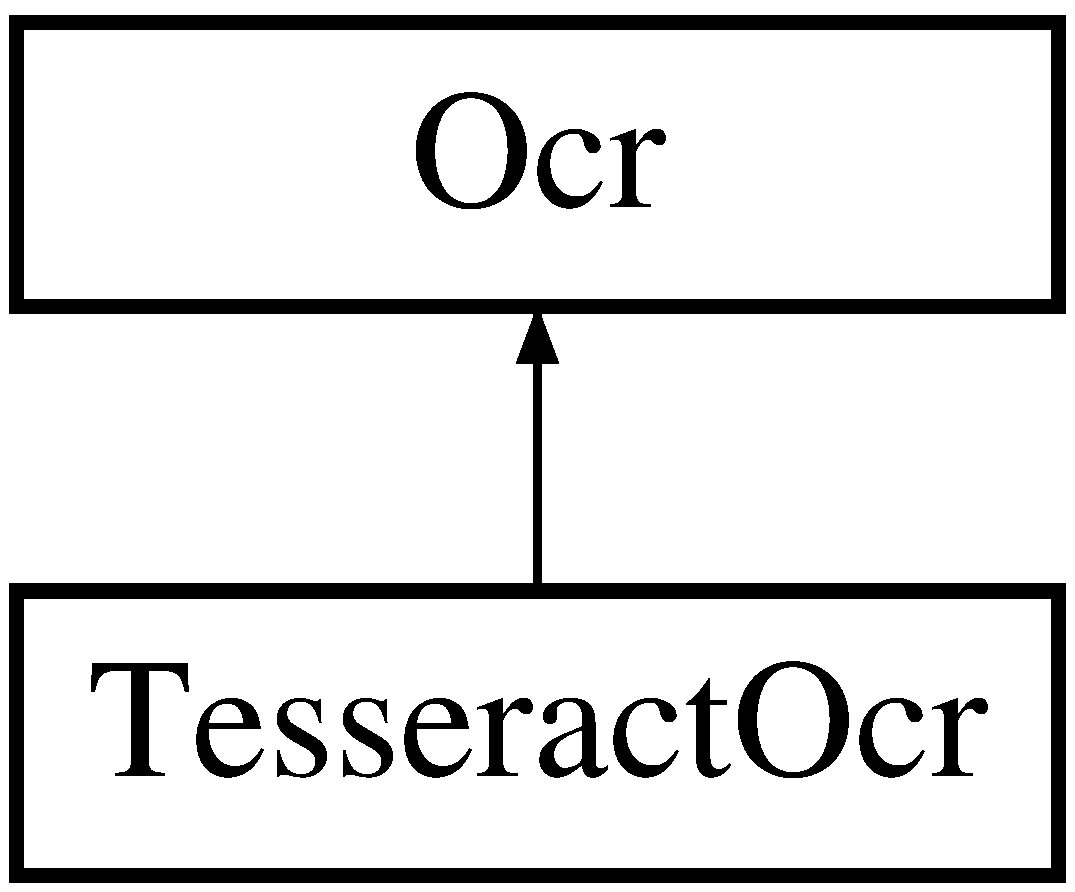
\includegraphics[height=2.000000cm]{classOcr}
\end{center}
\end{figure}
\subsection*{Public Member Functions}
\begin{DoxyCompactItemize}
\item 
\mbox{\hyperlink{classOcr_a285da90c44b929a9883a461de3e6578d}{Ocr}} ()
\begin{DoxyCompactList}\small\item\em Creates an empty \mbox{\hyperlink{classOcr}{Ocr}} object. \end{DoxyCompactList}\item 
\mbox{\Hypertarget{classOcr_a93ead91f7b64663ce6ed71ca4542d2f7}\label{classOcr_a93ead91f7b64663ce6ed71ca4542d2f7}} 
\mbox{\hyperlink{classOcr_a93ead91f7b64663ce6ed71ca4542d2f7}{$\sim$\+Ocr}} ()
\begin{DoxyCompactList}\small\item\em Destroys the ocr instance. \end{DoxyCompactList}\item 
virtual Q\+String\+List \mbox{\hyperlink{classOcr_a09a27b3a1f579c41ebda05f2a2cf4fed}{extract}} ()=0
\begin{DoxyCompactList}\small\item\em Extracts strings contained in the image. \end{DoxyCompactList}\item 
virtual Q\+String\+List \mbox{\hyperlink{classOcr_a1b0eed20f8e7f553401834849d044bd2}{get\+Available\+Languages}} () const =0
\begin{DoxyCompactList}\small\item\em Returns all available languages that can be used to extract strings from image. \end{DoxyCompactList}\item 
virtual Q\+String\+List \mbox{\hyperlink{classOcr_abf98eb2648c41446700515c3e6ed3a24}{get\+Languages}} () const
\begin{DoxyCompactList}\small\item\em Returns set languages to extract strings from image. \end{DoxyCompactList}\item 
virtual bool \mbox{\hyperlink{classOcr_ad2fb764c1c6766233ebbb53e62064bb8}{add\+Language}} (const Q\+String \&language)
\begin{DoxyCompactList}\small\item\em Add a language to try recognize characters in the image. \end{DoxyCompactList}\item 
virtual bool \mbox{\hyperlink{classOcr_a76001048da750374c987bef8171f1977}{remove\+Language}} (const Q\+String \&language)
\begin{DoxyCompactList}\small\item\em Remove a language to try recognize characters in the image. \end{DoxyCompactList}\item 
virtual bool \mbox{\hyperlink{classOcr_a0c9ebb9b531bdcd6789d4bf9cffb1d42}{is\+Available\+Language}} (const Q\+String \&language)
\begin{DoxyCompactList}\small\item\em Returns true if the language received by parameter is available to be used in the recognition, otherwise, returns false. \end{DoxyCompactList}\item 
Q\+String \mbox{\hyperlink{classOcr_a4bd4275b9b0503dd23dd553b4c0ef54c}{get\+Image}} () const
\begin{DoxyCompactList}\small\item\em Returns the path of image configured to recognize characters in. \end{DoxyCompactList}\item 
void \mbox{\hyperlink{classOcr_acdc41b9a0663c194d0fbede8c26ea319}{set\+Image}} (const Q\+String \&image)
\begin{DoxyCompactList}\small\item\em Sets the image path where try to recognize characters. \end{DoxyCompactList}\item 
Q\+String \mbox{\hyperlink{classOcr_a44f623335f8c26cc956b549a7bbf75fe}{get\+Data\+Path}} () const
\begin{DoxyCompactList}\small\item\em Returns folder path where are languages files. \end{DoxyCompactList}\item 
void \mbox{\hyperlink{classOcr_a0ec269340072accaa9d0932699b2a8ef}{set\+Data\+Path}} (const Q\+String \&datapath)
\begin{DoxyCompactList}\small\item\em Sets folder path where are languages files. \end{DoxyCompactList}\end{DoxyCompactItemize}
\subsection*{Protected Member Functions}
\begin{DoxyCompactItemize}
\item 
virtual Q\+String\+List \mbox{\hyperlink{classOcr_ac6f28693948e68e8958f1a27c73c79d1}{process\+Extration}} (const Q\+String \&source)=0
\begin{DoxyCompactList}\small\item\em Processes the text received by parameted. \end{DoxyCompactList}\end{DoxyCompactItemize}
\subsection*{Protected Attributes}
\begin{DoxyCompactItemize}
\item 
\mbox{\Hypertarget{classOcr_a731be039b828dfb1c1f3d5efdeaea9aa}\label{classOcr_a731be039b828dfb1c1f3d5efdeaea9aa}} 
Q\+File \mbox{\hyperlink{classOcr_a731be039b828dfb1c1f3d5efdeaea9aa}{image\+\_\+}}
\begin{DoxyCompactList}\small\item\em Image where will try to detect strings. \end{DoxyCompactList}\item 
\mbox{\Hypertarget{classOcr_ad5f11045f50c9d8a23d2cea235c509ad}\label{classOcr_ad5f11045f50c9d8a23d2cea235c509ad}} 
Q\+String \mbox{\hyperlink{classOcr_ad5f11045f50c9d8a23d2cea235c509ad}{language\+\_\+}}
\begin{DoxyCompactList}\small\item\em Languagues used to detect. \end{DoxyCompactList}\item 
\mbox{\Hypertarget{classOcr_a5c13f164c431cb4bc5a487eba75be7b4}\label{classOcr_a5c13f164c431cb4bc5a487eba75be7b4}} 
Q\+String \mbox{\hyperlink{classOcr_a5c13f164c431cb4bc5a487eba75be7b4}{datapath\+\_\+}}
\begin{DoxyCompactList}\small\item\em Path where are languages files. \end{DoxyCompactList}\end{DoxyCompactItemize}


\subsection{Detailed Description}
This is an interface for a optical character recognition api. 

Definition at line 23 of file ocr.\+h.



\subsection{Constructor \& Destructor Documentation}
\mbox{\Hypertarget{classOcr_a285da90c44b929a9883a461de3e6578d}\label{classOcr_a285da90c44b929a9883a461de3e6578d}} 
\index{Ocr@{Ocr}!Ocr@{Ocr}}
\index{Ocr@{Ocr}!Ocr@{Ocr}}
\subsubsection{\texorpdfstring{Ocr()}{Ocr()}}
{\footnotesize\ttfamily Ocr\+::\+Ocr (\begin{DoxyParamCaption}{ }\end{DoxyParamCaption})}



Creates an empty \mbox{\hyperlink{classOcr}{Ocr}} object. 

Sets default values. $<$ Default language always \char`\"{}eng\char`\"{}. 

Definition at line 13 of file ocr.\+cpp.



\subsection{Member Function Documentation}
\mbox{\Hypertarget{classOcr_ad2fb764c1c6766233ebbb53e62064bb8}\label{classOcr_ad2fb764c1c6766233ebbb53e62064bb8}} 
\index{Ocr@{Ocr}!add\+Language@{add\+Language}}
\index{add\+Language@{add\+Language}!Ocr@{Ocr}}
\subsubsection{\texorpdfstring{add\+Language()}{addLanguage()}}
{\footnotesize\ttfamily bool Ocr\+::add\+Language (\begin{DoxyParamCaption}\item[{const Q\+String \&}]{language }\end{DoxyParamCaption})\hspace{0.3cm}{\ttfamily [virtual]}}



Add a language to try recognize characters in the image. 

Check if the string recieved is an available language. Return true if the lenguage is added, if not return false.


\begin{DoxyParams}{Parameters}
{\em lang} & Q\+String that contains the language to add. \\
\hline
\end{DoxyParams}
\begin{DoxyReturn}{Returns}
true$\vert$false 
\end{DoxyReturn}


Definition at line 28 of file ocr.\+cpp.

\mbox{\Hypertarget{classOcr_a09a27b3a1f579c41ebda05f2a2cf4fed}\label{classOcr_a09a27b3a1f579c41ebda05f2a2cf4fed}} 
\index{Ocr@{Ocr}!extract@{extract}}
\index{extract@{extract}!Ocr@{Ocr}}
\subsubsection{\texorpdfstring{extract()}{extract()}}
{\footnotesize\ttfamily virtual Q\+String\+List Ocr\+::extract (\begin{DoxyParamCaption}{ }\end{DoxyParamCaption})\hspace{0.3cm}{\ttfamily [pure virtual]}}



Extracts strings contained in the image. 

Returns a Q\+Strings\+List containing the strings detected in the image. \begin{DoxyReturn}{Returns}
Strings list with strings extracted. 
\end{DoxyReturn}


Implemented in \mbox{\hyperlink{classTesseractOcr_a7e5a1d3e275f710ce187bc1c0b080327}{Tesseract\+Ocr}}.

\mbox{\Hypertarget{classOcr_a1b0eed20f8e7f553401834849d044bd2}\label{classOcr_a1b0eed20f8e7f553401834849d044bd2}} 
\index{Ocr@{Ocr}!get\+Available\+Languages@{get\+Available\+Languages}}
\index{get\+Available\+Languages@{get\+Available\+Languages}!Ocr@{Ocr}}
\subsubsection{\texorpdfstring{get\+Available\+Languages()}{getAvailableLanguages()}}
{\footnotesize\ttfamily virtual Q\+String\+List Ocr\+::get\+Available\+Languages (\begin{DoxyParamCaption}{ }\end{DoxyParamCaption}) const\hspace{0.3cm}{\ttfamily [pure virtual]}}



Returns all available languages that can be used to extract strings from image. 

\begin{DoxyReturn}{Returns}
List with all available languages. 
\end{DoxyReturn}


Implemented in \mbox{\hyperlink{classTesseractOcr_ad3486dcaa8a478c72ebaf76c43671326}{Tesseract\+Ocr}}.

\mbox{\Hypertarget{classOcr_a44f623335f8c26cc956b549a7bbf75fe}\label{classOcr_a44f623335f8c26cc956b549a7bbf75fe}} 
\index{Ocr@{Ocr}!get\+Data\+Path@{get\+Data\+Path}}
\index{get\+Data\+Path@{get\+Data\+Path}!Ocr@{Ocr}}
\subsubsection{\texorpdfstring{get\+Data\+Path()}{getDataPath()}}
{\footnotesize\ttfamily Q\+String Ocr\+::get\+Data\+Path (\begin{DoxyParamCaption}{ }\end{DoxyParamCaption}) const}



Returns folder path where are languages files. 

\begin{DoxyReturn}{Returns}
Folder path. 
\end{DoxyReturn}


Definition at line 74 of file ocr.\+cpp.

\mbox{\Hypertarget{classOcr_a4bd4275b9b0503dd23dd553b4c0ef54c}\label{classOcr_a4bd4275b9b0503dd23dd553b4c0ef54c}} 
\index{Ocr@{Ocr}!get\+Image@{get\+Image}}
\index{get\+Image@{get\+Image}!Ocr@{Ocr}}
\subsubsection{\texorpdfstring{get\+Image()}{getImage()}}
{\footnotesize\ttfamily Q\+String Ocr\+::get\+Image (\begin{DoxyParamCaption}{ }\end{DoxyParamCaption}) const}



Returns the path of image configured to recognize characters in. 

\begin{DoxyReturn}{Returns}
Image path. 
\end{DoxyReturn}


Definition at line 64 of file ocr.\+cpp.

\mbox{\Hypertarget{classOcr_abf98eb2648c41446700515c3e6ed3a24}\label{classOcr_abf98eb2648c41446700515c3e6ed3a24}} 
\index{Ocr@{Ocr}!get\+Languages@{get\+Languages}}
\index{get\+Languages@{get\+Languages}!Ocr@{Ocr}}
\subsubsection{\texorpdfstring{get\+Languages()}{getLanguages()}}
{\footnotesize\ttfamily Q\+String\+List Ocr\+::get\+Languages (\begin{DoxyParamCaption}{ }\end{DoxyParamCaption}) const\hspace{0.3cm}{\ttfamily [virtual]}}



Returns set languages to extract strings from image. 

\begin{DoxyReturn}{Returns}
List with set languages. 
\end{DoxyReturn}


Definition at line 23 of file ocr.\+cpp.

\mbox{\Hypertarget{classOcr_a0c9ebb9b531bdcd6789d4bf9cffb1d42}\label{classOcr_a0c9ebb9b531bdcd6789d4bf9cffb1d42}} 
\index{Ocr@{Ocr}!is\+Available\+Language@{is\+Available\+Language}}
\index{is\+Available\+Language@{is\+Available\+Language}!Ocr@{Ocr}}
\subsubsection{\texorpdfstring{is\+Available\+Language()}{isAvailableLanguage()}}
{\footnotesize\ttfamily bool Ocr\+::is\+Available\+Language (\begin{DoxyParamCaption}\item[{const Q\+String \&}]{language }\end{DoxyParamCaption})\hspace{0.3cm}{\ttfamily [virtual]}}



Returns true if the language received by parameter is available to be used in the recognition, otherwise, returns false. 


\begin{DoxyParams}{Parameters}
{\em language} & \mbox{\hyperlink{classString}{String}} language to check. \\
\hline
\end{DoxyParams}
\begin{DoxyReturn}{Returns}
bool 
\end{DoxyReturn}


Reimplemented in \mbox{\hyperlink{classTesseractOcr_aefe201ace3b144cb8834931b57f79bfd}{Tesseract\+Ocr}}.



Definition at line 57 of file ocr.\+cpp.

\mbox{\Hypertarget{classOcr_ac6f28693948e68e8958f1a27c73c79d1}\label{classOcr_ac6f28693948e68e8958f1a27c73c79d1}} 
\index{Ocr@{Ocr}!process\+Extration@{process\+Extration}}
\index{process\+Extration@{process\+Extration}!Ocr@{Ocr}}
\subsubsection{\texorpdfstring{process\+Extration()}{processExtration()}}
{\footnotesize\ttfamily Q\+String\+List Ocr\+::process\+Extration (\begin{DoxyParamCaption}\item[{const Q\+String \&}]{source }\end{DoxyParamCaption})\hspace{0.3cm}{\ttfamily [protected]}, {\ttfamily [pure virtual]}}



Processes the text received by parameted. 

Split the string in phrases and returns a list with phrases contained in source. 
\begin{DoxyParams}{Parameters}
{\em source} & \\
\hline
\end{DoxyParams}
\begin{DoxyReturn}{Returns}

\end{DoxyReturn}


Definition at line 84 of file ocr.\+cpp.

\mbox{\Hypertarget{classOcr_a76001048da750374c987bef8171f1977}\label{classOcr_a76001048da750374c987bef8171f1977}} 
\index{Ocr@{Ocr}!remove\+Language@{remove\+Language}}
\index{remove\+Language@{remove\+Language}!Ocr@{Ocr}}
\subsubsection{\texorpdfstring{remove\+Language()}{removeLanguage()}}
{\footnotesize\ttfamily bool Ocr\+::remove\+Language (\begin{DoxyParamCaption}\item[{const Q\+String \&}]{language }\end{DoxyParamCaption})\hspace{0.3cm}{\ttfamily [virtual]}}



Remove a language to try recognize characters in the image. 

Returns true if the language was removed succesfully, otherwise, returns false. 
\begin{DoxyParams}{Parameters}
{\em language} & \mbox{\hyperlink{classString}{String}} language to be removed. \\
\hline
\end{DoxyParams}
\begin{DoxyReturn}{Returns}
bool 
\end{DoxyReturn}


Definition at line 43 of file ocr.\+cpp.

\mbox{\Hypertarget{classOcr_a0ec269340072accaa9d0932699b2a8ef}\label{classOcr_a0ec269340072accaa9d0932699b2a8ef}} 
\index{Ocr@{Ocr}!set\+Data\+Path@{set\+Data\+Path}}
\index{set\+Data\+Path@{set\+Data\+Path}!Ocr@{Ocr}}
\subsubsection{\texorpdfstring{set\+Data\+Path()}{setDataPath()}}
{\footnotesize\ttfamily void Ocr\+::set\+Data\+Path (\begin{DoxyParamCaption}\item[{const Q\+String \&}]{datapath }\end{DoxyParamCaption})}



Sets folder path where are languages files. 


\begin{DoxyParams}{Parameters}
{\em datapath} & Folder path. \\
\hline
\end{DoxyParams}


Definition at line 79 of file ocr.\+cpp.

\mbox{\Hypertarget{classOcr_acdc41b9a0663c194d0fbede8c26ea319}\label{classOcr_acdc41b9a0663c194d0fbede8c26ea319}} 
\index{Ocr@{Ocr}!set\+Image@{set\+Image}}
\index{set\+Image@{set\+Image}!Ocr@{Ocr}}
\subsubsection{\texorpdfstring{set\+Image()}{setImage()}}
{\footnotesize\ttfamily void Ocr\+::set\+Image (\begin{DoxyParamCaption}\item[{const Q\+String \&}]{image }\end{DoxyParamCaption})}



Sets the image path where try to recognize characters. 


\begin{DoxyParams}{Parameters}
{\em image} & Path of image. \\
\hline
\end{DoxyParams}


Definition at line 69 of file ocr.\+cpp.



The documentation for this class was generated from the following files\+:\begin{DoxyCompactItemize}
\item 
src/optical\+\_\+character\+\_\+recognition/\mbox{\hyperlink{ocr_8h}{ocr.\+h}}\item 
src/optical\+\_\+character\+\_\+recognition/\mbox{\hyperlink{ocr_8cpp}{ocr.\+cpp}}\end{DoxyCompactItemize}

\hypertarget{classString}{}\section{String Class Reference}
\label{classString}\index{String@{String}}


This is the representation of a string with their properties.  




{\ttfamily \#include $<$string.\+h$>$}

Inheritance diagram for String\+:\begin{figure}[H]
\begin{center}
\leavevmode
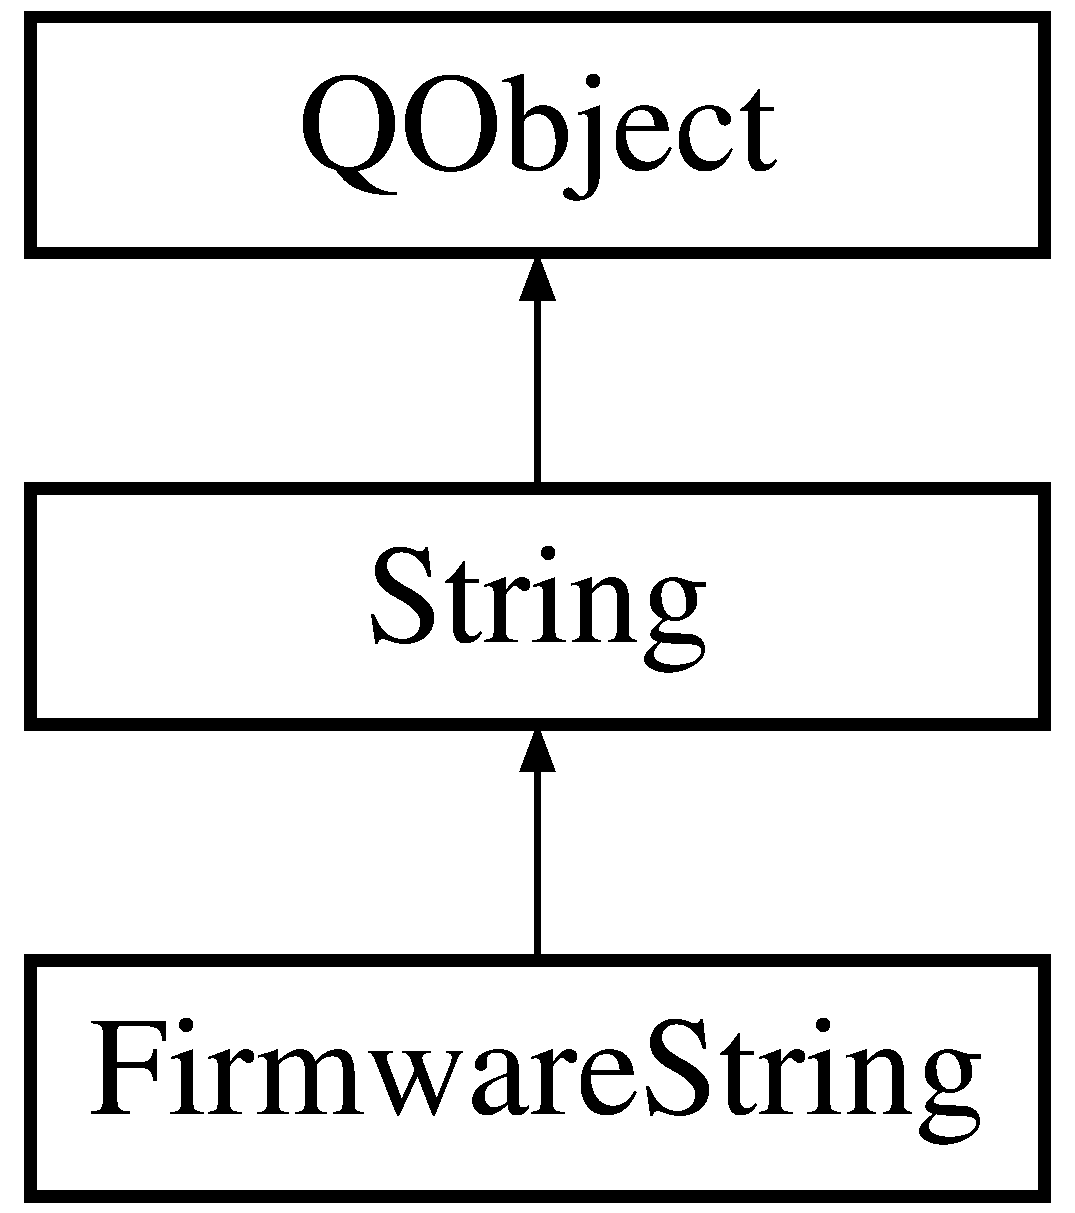
\includegraphics[height=3.000000cm]{classString}
\end{center}
\end{figure}
\subsection*{Signals}
\begin{DoxyCompactItemize}
\item 
\mbox{\Hypertarget{classString_a96493c66757b6aa5a5ac45c245d84740}\label{classString_a96493c66757b6aa5a5ac45c245d84740}} 
void \mbox{\hyperlink{classString_a96493c66757b6aa5a5ac45c245d84740}{id\+Changed}} ()
\begin{DoxyCompactList}\small\item\em The signal is emitted when the identifier of the string has changed. \end{DoxyCompactList}\item 
\mbox{\Hypertarget{classString_aa0c62ee31f5e0e91b8f68a13405db51b}\label{classString_aa0c62ee31f5e0e91b8f68a13405db51b}} 
void \mbox{\hyperlink{classString_aa0c62ee31f5e0e91b8f68a13405db51b}{value\+Changed}} ()
\begin{DoxyCompactList}\small\item\em The signal is emitted when the value of the string has changed. \end{DoxyCompactList}\item 
\mbox{\Hypertarget{classString_ada21cf632b6350cd959efc3b7c0a1b5f}\label{classString_ada21cf632b6350cd959efc3b7c0a1b5f}} 
void \mbox{\hyperlink{classString_ada21cf632b6350cd959efc3b7c0a1b5f}{description\+Changed}} ()
\begin{DoxyCompactList}\small\item\em The signal is emitted when the description of the string has changed. \end{DoxyCompactList}\item 
\mbox{\Hypertarget{classString_ae48fd165246597a387bcdc86aede6899}\label{classString_ae48fd165246597a387bcdc86aede6899}} 
void \mbox{\hyperlink{classString_ae48fd165246597a387bcdc86aede6899}{max\+Length\+Changed}} ()
\begin{DoxyCompactList}\small\item\em The signal is emitted when the max length of the string has changed. \end{DoxyCompactList}\item 
\mbox{\Hypertarget{classString_a9ffcae019b2cfb3a5e75ba4d390d725b}\label{classString_a9ffcae019b2cfb3a5e75ba4d390d725b}} 
void \mbox{\hyperlink{classString_a9ffcae019b2cfb3a5e75ba4d390d725b}{state\+Changed}} ()
\begin{DoxyCompactList}\small\item\em The signal is emitted when the state of the string has changed. \end{DoxyCompactList}\item 
\mbox{\Hypertarget{classString_ab6012061024cd0862b9a8ca9fbc1896d}\label{classString_ab6012061024cd0862b9a8ca9fbc1896d}} 
void \mbox{\hyperlink{classString_ab6012061024cd0862b9a8ca9fbc1896d}{selected\+Changed}} ()
\begin{DoxyCompactList}\small\item\em The signal is emitted when the string is selected or unselected. \end{DoxyCompactList}\item 
\mbox{\Hypertarget{classString_a9f37720f465dce86576a2ad347c386b0}\label{classString_a9f37720f465dce86576a2ad347c386b0}} 
void \mbox{\hyperlink{classString_a9f37720f465dce86576a2ad347c386b0}{editable\+Changed}} ()
\begin{DoxyCompactList}\small\item\em The signal is emitted when the editable parameter is changed. \end{DoxyCompactList}\end{DoxyCompactItemize}
\subsection*{Public Member Functions}
\begin{DoxyCompactItemize}
\item 
\mbox{\Hypertarget{classString_a8a7ef356e05eb9b1ea1ab518baee3095}\label{classString_a8a7ef356e05eb9b1ea1ab518baee3095}} 
\mbox{\hyperlink{classString_a8a7ef356e05eb9b1ea1ab518baee3095}{String}} ()
\begin{DoxyCompactList}\small\item\em Constructs an empty string. \end{DoxyCompactList}\item 
\mbox{\hyperlink{classString_addd6bcc4ba529bdc45d3fd69ad1a3569}{String}} (\mbox{\hyperlink{classString}{String}} \&other)
\begin{DoxyCompactList}\small\item\em Constructs a string replic from another received by parameter. \end{DoxyCompactList}\item 
\mbox{\hyperlink{classString_a4edf46375241ec3585f26758750b3d9e}{String}} (const Q\+String \&id, const Q\+String \&value, const Q\+String \&description, const Q\+String \&max\+Length, const Q\+String \&state, const bool selected=false, const bool editable=true)
\begin{DoxyCompactList}\small\item\em Constructs a string with diferents value members received by parameter. \end{DoxyCompactList}\item 
Q\+String \mbox{\hyperlink{classString_ab32615121278a445dba468c7ef18ee7a}{get\+Id}} () const
\begin{DoxyCompactList}\small\item\em Returns the identifier of the string. \end{DoxyCompactList}\item 
bool \mbox{\hyperlink{classString_a11c7a52caa2ebc68d27ecd9cb5a35d16}{set\+Id}} (const Q\+String \&id)
\begin{DoxyCompactList}\small\item\em Sets the identifier of the string. \end{DoxyCompactList}\item 
Q\+String \mbox{\hyperlink{classString_a926f7c30cfca26009604d0c765950c4b}{get\+Value}} () const
\begin{DoxyCompactList}\small\item\em Returns the value of the string. \end{DoxyCompactList}\item 
bool \mbox{\hyperlink{classString_ae863781e31fe2378468547159a9172a6}{set\+Value}} (const Q\+String \&value)
\begin{DoxyCompactList}\small\item\em Sets the value of the string. \end{DoxyCompactList}\item 
Q\+String \mbox{\hyperlink{classString_ae604e3af13ef6ba3113a7484edfc3c55}{get\+Description}} () const
\begin{DoxyCompactList}\small\item\em Returns the description of the string. \end{DoxyCompactList}\item 
bool \mbox{\hyperlink{classString_ac91f0504a470b1602952cfd657979e4b}{set\+Description}} (const Q\+String \&description)
\begin{DoxyCompactList}\small\item\em Sets the description of the string. \end{DoxyCompactList}\item 
Q\+String \mbox{\hyperlink{classString_af95fe7d7e2a8b604d7af3b7f0476ec0e}{get\+Max\+Length}} () const
\begin{DoxyCompactList}\small\item\em Returns the max length of the string. \end{DoxyCompactList}\item 
bool \mbox{\hyperlink{classString_a141c695ac9095099e0d27a3f1b01a1ca}{set\+Max\+Length}} (const Q\+String \&max\+Length)
\begin{DoxyCompactList}\small\item\em Sets the max length of the string. \end{DoxyCompactList}\item 
Q\+String \mbox{\hyperlink{classString_ae5ee38919f5a360e0283baedb11c48e0}{get\+State}} () const
\begin{DoxyCompactList}\small\item\em Returns the state of the string. \end{DoxyCompactList}\item 
bool \mbox{\hyperlink{classString_a7b1b070889aef0e2e9eb4d7d55161cf3}{set\+State}} (const Q\+String \&state)
\begin{DoxyCompactList}\small\item\em Sets the state of the string. \end{DoxyCompactList}\item 
bool \mbox{\hyperlink{classString_a43fe9257fb504215834afa322313f8c9}{is\+Empty}} ()
\begin{DoxyCompactList}\small\item\em Returns true if string is empty. \end{DoxyCompactList}\item 
bool \mbox{\hyperlink{classString_a3f5ffd092dd9870ae281b2e08d3b69dd}{is\+Selected}} () const
\begin{DoxyCompactList}\small\item\em Returns true if string is selected, else returns false. \end{DoxyCompactList}\item 
\mbox{\Hypertarget{classString_ad575beeccbf4ae38bc5eab1ebfff3216}\label{classString_ad575beeccbf4ae38bc5eab1ebfff3216}} 
void \mbox{\hyperlink{classString_ad575beeccbf4ae38bc5eab1ebfff3216}{select}} ()
\begin{DoxyCompactList}\small\item\em Changes the string to selected. \end{DoxyCompactList}\item 
\mbox{\Hypertarget{classString_a26bc857fbf7077d23667cd0b1e9ecd6d}\label{classString_a26bc857fbf7077d23667cd0b1e9ecd6d}} 
void \mbox{\hyperlink{classString_a26bc857fbf7077d23667cd0b1e9ecd6d}{unselect}} ()
\begin{DoxyCompactList}\small\item\em Changes the string to unselected. \end{DoxyCompactList}\item 
void \mbox{\hyperlink{classString_a68737226a49a262c0a4952473788a77a}{set\+Selected}} (bool selected)
\begin{DoxyCompactList}\small\item\em Changes the string to selected or unselected depending on the value received by parameter. \end{DoxyCompactList}\item 
bool \mbox{\hyperlink{classString_a64c436144f008a40743c64b5094700bb}{is\+Editable}} () const
\begin{DoxyCompactList}\small\item\em Returns the editable state of the string. \end{DoxyCompactList}\item 
void \mbox{\hyperlink{classString_ae2ff38f8907c105ef577012a8db3f46e}{set\+Editable}} (bool editable)
\begin{DoxyCompactList}\small\item\em Sets the editable parameter of the string. \end{DoxyCompactList}\item 
Q\+String \mbox{\hyperlink{classString_ab73513e47b7572940944d54963056d07}{to\+Fp\+File\+Format}} () const
\begin{DoxyCompactList}\small\item\em Returns the model converted to a string with the format in file fp. \end{DoxyCompactList}\item 
Q\+String \mbox{\hyperlink{classString_a3dca5b8881d9f531a7ee9bbaf2fff535}{to\+Json}} (Q\+Json\+Document\+::\+Json\+Format format=Q\+Json\+Document\+::\+Compact)
\begin{DoxyCompactList}\small\item\em Returns the string converted to a J\+S\+ON Q\+String. \end{DoxyCompactList}\item 
Q\+Json\+Object \mbox{\hyperlink{classString_a44e35d48e6bf3efe128d3855d242a131}{to\+Json\+Object}} ()
\begin{DoxyCompactList}\small\item\em Returns the string converted to a \#\+Q\+Json\+Object. \end{DoxyCompactList}\item 
\mbox{\hyperlink{classString}{String}} \& \mbox{\hyperlink{classString_a734f34a0b7a42bcad30c368d6e8c5469}{operator=}} (const \mbox{\hyperlink{classString}{String}} \&other)
\begin{DoxyCompactList}\small\item\em Assigns other to string and returns a reference to this string. \end{DoxyCompactList}\end{DoxyCompactItemize}
\subsection*{Static Public Member Functions}
\begin{DoxyCompactItemize}
\item 
static \mbox{\hyperlink{classString}{String}} $\ast$ \mbox{\hyperlink{classString_af406afb78e8dae5e7d2deef41d1f9ed7}{from\+Json}} (Q\+String \&json)
\begin{DoxyCompactList}\small\item\em Returns a \mbox{\hyperlink{classString}{String}} initializated with the J\+S\+ON string json. \end{DoxyCompactList}\item 
static \mbox{\hyperlink{classString}{String}} $\ast$ \mbox{\hyperlink{classString_ab785f3109ff1638b4fb2b052de6cac03}{from\+Json}} (Q\+Byte\+Array \&json)
\begin{DoxyCompactList}\small\item\em Returns a \mbox{\hyperlink{classString}{String}} initializated with the \#\+Q\+Byte\+Array data json. \end{DoxyCompactList}\end{DoxyCompactItemize}
\subsection*{Protected Attributes}
\begin{DoxyCompactItemize}
\item 
\mbox{\Hypertarget{classString_a57119b0e8878311777ccf94ea542f745}\label{classString_a57119b0e8878311777ccf94ea542f745}} 
Q\+String {\bfseries id\+\_\+}
\item 
\mbox{\Hypertarget{classString_a4168491f40c415cd410fbab1cccfc523}\label{classString_a4168491f40c415cd410fbab1cccfc523}} 
Q\+String {\bfseries value\+\_\+}
\item 
\mbox{\Hypertarget{classString_a87cbb04e3c7fd009a4323e95d39cfd1e}\label{classString_a87cbb04e3c7fd009a4323e95d39cfd1e}} 
Q\+String {\bfseries description\+\_\+}
\item 
\mbox{\Hypertarget{classString_a8463d3d3d595bc50b4f37908f4e6aa74}\label{classString_a8463d3d3d595bc50b4f37908f4e6aa74}} 
Q\+String {\bfseries max\+Length\+\_\+}
\item 
\mbox{\Hypertarget{classString_acb000d4634c91cdffcc89e44c534c008}\label{classString_acb000d4634c91cdffcc89e44c534c008}} 
Q\+String {\bfseries state\+\_\+}
\item 
\mbox{\Hypertarget{classString_a2c7623a98c3bec1ae8658952dca0b1bf}\label{classString_a2c7623a98c3bec1ae8658952dca0b1bf}} 
bool {\bfseries selected\+\_\+}
\item 
\mbox{\Hypertarget{classString_ac8f7b0d152b7aaedb6eadb2c15ed23b5}\label{classString_ac8f7b0d152b7aaedb6eadb2c15ed23b5}} 
bool {\bfseries editable\+\_\+}
\end{DoxyCompactItemize}
\subsection*{Properties}
\begin{DoxyCompactItemize}
\item 
\mbox{\Hypertarget{classString_a82cd6049ff79198e7d24ed97b7a6c4c3}\label{classString_a82cd6049ff79198e7d24ed97b7a6c4c3}} 
Q\+String {\bfseries id}
\item 
\mbox{\Hypertarget{classString_a08d78cc301801cdac26795f3070fab9c}\label{classString_a08d78cc301801cdac26795f3070fab9c}} 
Q\+String {\bfseries value}
\item 
\mbox{\Hypertarget{classString_aa3d3e472e670f550eb5f9e26aeee81d6}\label{classString_aa3d3e472e670f550eb5f9e26aeee81d6}} 
Q\+String {\bfseries description}
\item 
\mbox{\Hypertarget{classString_a7a711e734960d3e721a6439d96289ce2}\label{classString_a7a711e734960d3e721a6439d96289ce2}} 
Q\+String {\bfseries max\+Length}
\item 
\mbox{\Hypertarget{classString_ab4d9446f69355dc0c9bdd3ecda847679}\label{classString_ab4d9446f69355dc0c9bdd3ecda847679}} 
Q\+String {\bfseries state}
\item 
\mbox{\Hypertarget{classString_aa80dde9547a7d229060f9bb094ee28f1}\label{classString_aa80dde9547a7d229060f9bb094ee28f1}} 
bool {\bfseries selected}
\item 
\mbox{\Hypertarget{classString_a11a02211f65634f17ea47cb8b1a272ed}\label{classString_a11a02211f65634f17ea47cb8b1a272ed}} 
bool {\bfseries editable}
\end{DoxyCompactItemize}


\subsection{Detailed Description}
This is the representation of a string with their properties. 

Definition at line 19 of file string.\+h.



\subsection{Constructor \& Destructor Documentation}
\mbox{\Hypertarget{classString_addd6bcc4ba529bdc45d3fd69ad1a3569}\label{classString_addd6bcc4ba529bdc45d3fd69ad1a3569}} 
\index{String@{String}!String@{String}}
\index{String@{String}!String@{String}}
\subsubsection{\texorpdfstring{String()}{String()}\hspace{0.1cm}{\footnotesize\ttfamily [1/2]}}
{\footnotesize\ttfamily String\+::\+String (\begin{DoxyParamCaption}\item[{\mbox{\hyperlink{classString}{String}} \&}]{other }\end{DoxyParamCaption})}



Constructs a string replic from another received by parameter. 


\begin{DoxyParams}{Parameters}
{\em other} & string to be duplicated. \\
\hline
\end{DoxyParams}


Definition at line 23 of file string.\+cpp.

\mbox{\Hypertarget{classString_a4edf46375241ec3585f26758750b3d9e}\label{classString_a4edf46375241ec3585f26758750b3d9e}} 
\index{String@{String}!String@{String}}
\index{String@{String}!String@{String}}
\subsubsection{\texorpdfstring{String()}{String()}\hspace{0.1cm}{\footnotesize\ttfamily [2/2]}}
{\footnotesize\ttfamily String\+::\+String (\begin{DoxyParamCaption}\item[{const Q\+String \&}]{id,  }\item[{const Q\+String \&}]{value,  }\item[{const Q\+String \&}]{description,  }\item[{const Q\+String \&}]{max\+Length,  }\item[{const Q\+String \&}]{state,  }\item[{const bool}]{selected = {\ttfamily false},  }\item[{const bool}]{editable = {\ttfamily true} }\end{DoxyParamCaption})}



Constructs a string with diferents value members received by parameter. 


\begin{DoxyParams}{Parameters}
{\em id} & \mbox{\hyperlink{classString}{String}} identifier. \\
\hline
{\em value} & \mbox{\hyperlink{classString}{String}} value. \\
\hline
{\em description} & \mbox{\hyperlink{classString}{String}} description. \\
\hline
{\em max\+Length} & \mbox{\hyperlink{classString}{String}} max\+Length. \\
\hline
{\em state} & \mbox{\hyperlink{classString}{String}} state. \\
\hline
{\em selected} & \mbox{\hyperlink{classString}{String}} selected. \\
\hline
{\em editable} & \mbox{\hyperlink{classString}{String}} editable state. \\
\hline
\end{DoxyParams}


Definition at line 34 of file string.\+cpp.



\subsection{Member Function Documentation}
\mbox{\Hypertarget{classString_af406afb78e8dae5e7d2deef41d1f9ed7}\label{classString_af406afb78e8dae5e7d2deef41d1f9ed7}} 
\index{String@{String}!from\+Json@{from\+Json}}
\index{from\+Json@{from\+Json}!String@{String}}
\subsubsection{\texorpdfstring{from\+Json()}{fromJson()}\hspace{0.1cm}{\footnotesize\ttfamily [1/2]}}
{\footnotesize\ttfamily \mbox{\hyperlink{classString}{String}} $\ast$ String\+::from\+Json (\begin{DoxyParamCaption}\item[{Q\+String \&}]{json }\end{DoxyParamCaption})\hspace{0.3cm}{\ttfamily [static]}}



Returns a \mbox{\hyperlink{classString}{String}} initializated with the J\+S\+ON string json. 

If the J\+S\+ON data received is not valid, return an empty model. 
\begin{DoxyParams}{Parameters}
{\em json} & \mbox{\hyperlink{classString}{String}} in J\+S\+ON format to be converted. \\
\hline
\end{DoxyParams}
\begin{DoxyReturn}{Returns}
\mbox{\hyperlink{classContextualizationModel}{Contextualization\+Model}} 
\end{DoxyReturn}


Definition at line 218 of file string.\+cpp.

\mbox{\Hypertarget{classString_ab785f3109ff1638b4fb2b052de6cac03}\label{classString_ab785f3109ff1638b4fb2b052de6cac03}} 
\index{String@{String}!from\+Json@{from\+Json}}
\index{from\+Json@{from\+Json}!String@{String}}
\subsubsection{\texorpdfstring{from\+Json()}{fromJson()}\hspace{0.1cm}{\footnotesize\ttfamily [2/2]}}
{\footnotesize\ttfamily \mbox{\hyperlink{classString}{String}} $\ast$ String\+::from\+Json (\begin{DoxyParamCaption}\item[{Q\+Byte\+Array \&}]{json }\end{DoxyParamCaption})\hspace{0.3cm}{\ttfamily [static]}}



Returns a \mbox{\hyperlink{classString}{String}} initializated with the \#\+Q\+Byte\+Array data json. 

If the J\+S\+ON data received is not valid, return an empty model. 
\begin{DoxyParams}{Parameters}
{\em json} & Q\+Byte\+Array in J\+S\+ON format to be converted. \\
\hline
\end{DoxyParams}
\begin{DoxyReturn}{Returns}
\mbox{\hyperlink{classString}{String}} 
\end{DoxyReturn}


Definition at line 225 of file string.\+cpp.

\mbox{\Hypertarget{classString_ae604e3af13ef6ba3113a7484edfc3c55}\label{classString_ae604e3af13ef6ba3113a7484edfc3c55}} 
\index{String@{String}!get\+Description@{get\+Description}}
\index{get\+Description@{get\+Description}!String@{String}}
\subsubsection{\texorpdfstring{get\+Description()}{getDescription()}}
{\footnotesize\ttfamily Q\+String String\+::get\+Description (\begin{DoxyParamCaption}{ }\end{DoxyParamCaption}) const}



Returns the description of the string. 

\begin{DoxyReturn}{Returns}
Description of the string. 
\end{DoxyReturn}


Definition at line 86 of file string.\+cpp.

\mbox{\Hypertarget{classString_ab32615121278a445dba468c7ef18ee7a}\label{classString_ab32615121278a445dba468c7ef18ee7a}} 
\index{String@{String}!get\+Id@{get\+Id}}
\index{get\+Id@{get\+Id}!String@{String}}
\subsubsection{\texorpdfstring{get\+Id()}{getId()}}
{\footnotesize\ttfamily Q\+String String\+::get\+Id (\begin{DoxyParamCaption}{ }\end{DoxyParamCaption}) const}



Returns the identifier of the string. 

\begin{DoxyReturn}{Returns}
Identifier of the string. 
\end{DoxyReturn}


Definition at line 52 of file string.\+cpp.

\mbox{\Hypertarget{classString_af95fe7d7e2a8b604d7af3b7f0476ec0e}\label{classString_af95fe7d7e2a8b604d7af3b7f0476ec0e}} 
\index{String@{String}!get\+Max\+Length@{get\+Max\+Length}}
\index{get\+Max\+Length@{get\+Max\+Length}!String@{String}}
\subsubsection{\texorpdfstring{get\+Max\+Length()}{getMaxLength()}}
{\footnotesize\ttfamily Q\+String String\+::get\+Max\+Length (\begin{DoxyParamCaption}{ }\end{DoxyParamCaption}) const}



Returns the max length of the string. 

\begin{DoxyReturn}{Returns}
Max length of the string. 
\end{DoxyReturn}


Definition at line 103 of file string.\+cpp.

\mbox{\Hypertarget{classString_ae5ee38919f5a360e0283baedb11c48e0}\label{classString_ae5ee38919f5a360e0283baedb11c48e0}} 
\index{String@{String}!get\+State@{get\+State}}
\index{get\+State@{get\+State}!String@{String}}
\subsubsection{\texorpdfstring{get\+State()}{getState()}}
{\footnotesize\ttfamily Q\+String String\+::get\+State (\begin{DoxyParamCaption}{ }\end{DoxyParamCaption}) const}



Returns the state of the string. 

\begin{DoxyReturn}{Returns}
State of the string. 
\end{DoxyReturn}


Definition at line 120 of file string.\+cpp.

\mbox{\Hypertarget{classString_a926f7c30cfca26009604d0c765950c4b}\label{classString_a926f7c30cfca26009604d0c765950c4b}} 
\index{String@{String}!get\+Value@{get\+Value}}
\index{get\+Value@{get\+Value}!String@{String}}
\subsubsection{\texorpdfstring{get\+Value()}{getValue()}}
{\footnotesize\ttfamily Q\+String String\+::get\+Value (\begin{DoxyParamCaption}{ }\end{DoxyParamCaption}) const}



Returns the value of the string. 

Returns true if the identifier was set, otherwise, returns false. \begin{DoxyReturn}{Returns}
Value of the string. 
\end{DoxyReturn}


Definition at line 69 of file string.\+cpp.

\mbox{\Hypertarget{classString_a64c436144f008a40743c64b5094700bb}\label{classString_a64c436144f008a40743c64b5094700bb}} 
\index{String@{String}!is\+Editable@{is\+Editable}}
\index{is\+Editable@{is\+Editable}!String@{String}}
\subsubsection{\texorpdfstring{is\+Editable()}{isEditable()}}
{\footnotesize\ttfamily bool String\+::is\+Editable (\begin{DoxyParamCaption}{ }\end{DoxyParamCaption}) const}



Returns the editable state of the string. 

\begin{DoxyReturn}{Returns}
Editable state of the string. 
\end{DoxyReturn}


Definition at line 172 of file string.\+cpp.

\mbox{\Hypertarget{classString_a43fe9257fb504215834afa322313f8c9}\label{classString_a43fe9257fb504215834afa322313f8c9}} 
\index{String@{String}!is\+Empty@{is\+Empty}}
\index{is\+Empty@{is\+Empty}!String@{String}}
\subsubsection{\texorpdfstring{is\+Empty()}{isEmpty()}}
{\footnotesize\ttfamily bool String\+::is\+Empty (\begin{DoxyParamCaption}{ }\end{DoxyParamCaption})}



Returns true if string is empty. 

A string is empty if has a null o empty value. \begin{DoxyReturn}{Returns}
bool 
\end{DoxyReturn}


Definition at line 137 of file string.\+cpp.

\mbox{\Hypertarget{classString_a3f5ffd092dd9870ae281b2e08d3b69dd}\label{classString_a3f5ffd092dd9870ae281b2e08d3b69dd}} 
\index{String@{String}!is\+Selected@{is\+Selected}}
\index{is\+Selected@{is\+Selected}!String@{String}}
\subsubsection{\texorpdfstring{is\+Selected()}{isSelected()}}
{\footnotesize\ttfamily bool String\+::is\+Selected (\begin{DoxyParamCaption}{ }\end{DoxyParamCaption}) const}



Returns true if string is selected, else returns false. 

\begin{DoxyReturn}{Returns}
bool 
\end{DoxyReturn}


Definition at line 146 of file string.\+cpp.

\mbox{\Hypertarget{classString_a734f34a0b7a42bcad30c368d6e8c5469}\label{classString_a734f34a0b7a42bcad30c368d6e8c5469}} 
\index{String@{String}!operator=@{operator=}}
\index{operator=@{operator=}!String@{String}}
\subsubsection{\texorpdfstring{operator=()}{operator=()}}
{\footnotesize\ttfamily \mbox{\hyperlink{classString}{String}} \& String\+::operator= (\begin{DoxyParamCaption}\item[{const \mbox{\hyperlink{classString}{String}} \&}]{other }\end{DoxyParamCaption})}



Assigns other to string and returns a reference to this string. 

Overloads from\+String(\+Q\+String \&json) function. 
\begin{DoxyParams}{Parameters}
{\em other} & Model to be copied. \\
\hline
\end{DoxyParams}
\begin{DoxyReturn}{Returns}
Reference to this string. 
\end{DoxyReturn}


Definition at line 262 of file string.\+cpp.

\mbox{\Hypertarget{classString_ac91f0504a470b1602952cfd657979e4b}\label{classString_ac91f0504a470b1602952cfd657979e4b}} 
\index{String@{String}!set\+Description@{set\+Description}}
\index{set\+Description@{set\+Description}!String@{String}}
\subsubsection{\texorpdfstring{set\+Description()}{setDescription()}}
{\footnotesize\ttfamily bool String\+::set\+Description (\begin{DoxyParamCaption}\item[{const Q\+String \&}]{description }\end{DoxyParamCaption})}



Sets the description of the string. 

Returns true if the description was set, otherwise, returns false. 
\begin{DoxyParams}{Parameters}
{\em description} & New description of the string. \\
\hline
\end{DoxyParams}


Definition at line 91 of file string.\+cpp.

\mbox{\Hypertarget{classString_ae2ff38f8907c105ef577012a8db3f46e}\label{classString_ae2ff38f8907c105ef577012a8db3f46e}} 
\index{String@{String}!set\+Editable@{set\+Editable}}
\index{set\+Editable@{set\+Editable}!String@{String}}
\subsubsection{\texorpdfstring{set\+Editable()}{setEditable()}}
{\footnotesize\ttfamily void String\+::set\+Editable (\begin{DoxyParamCaption}\item[{bool}]{editable }\end{DoxyParamCaption})}



Sets the editable parameter of the string. 


\begin{DoxyParams}{Parameters}
{\em state} & New editable state of the string. \\
\hline
\end{DoxyParams}


Definition at line 177 of file string.\+cpp.

\mbox{\Hypertarget{classString_a11c7a52caa2ebc68d27ecd9cb5a35d16}\label{classString_a11c7a52caa2ebc68d27ecd9cb5a35d16}} 
\index{String@{String}!set\+Id@{set\+Id}}
\index{set\+Id@{set\+Id}!String@{String}}
\subsubsection{\texorpdfstring{set\+Id()}{setId()}}
{\footnotesize\ttfamily bool String\+::set\+Id (\begin{DoxyParamCaption}\item[{const Q\+String \&}]{id }\end{DoxyParamCaption})}



Sets the identifier of the string. 


\begin{DoxyParams}{Parameters}
{\em id} & New identifier of the string. \\
\hline
\end{DoxyParams}


Definition at line 57 of file string.\+cpp.

\mbox{\Hypertarget{classString_a141c695ac9095099e0d27a3f1b01a1ca}\label{classString_a141c695ac9095099e0d27a3f1b01a1ca}} 
\index{String@{String}!set\+Max\+Length@{set\+Max\+Length}}
\index{set\+Max\+Length@{set\+Max\+Length}!String@{String}}
\subsubsection{\texorpdfstring{set\+Max\+Length()}{setMaxLength()}}
{\footnotesize\ttfamily bool String\+::set\+Max\+Length (\begin{DoxyParamCaption}\item[{const Q\+String \&}]{max\+Length }\end{DoxyParamCaption})}



Sets the max length of the string. 

Returns true if the max length was set, otherwise, returns false. 
\begin{DoxyParams}{Parameters}
{\em max\+Length} & New max length of the string. \\
\hline
\end{DoxyParams}


Definition at line 108 of file string.\+cpp.

\mbox{\Hypertarget{classString_a68737226a49a262c0a4952473788a77a}\label{classString_a68737226a49a262c0a4952473788a77a}} 
\index{String@{String}!set\+Selected@{set\+Selected}}
\index{set\+Selected@{set\+Selected}!String@{String}}
\subsubsection{\texorpdfstring{set\+Selected()}{setSelected()}}
{\footnotesize\ttfamily void String\+::set\+Selected (\begin{DoxyParamCaption}\item[{bool}]{selected }\end{DoxyParamCaption})}



Changes the string to selected or unselected depending on the value received by parameter. 


\begin{DoxyParams}{Parameters}
{\em selected} & New selection state of the string.. \\
\hline
\end{DoxyParams}


Definition at line 165 of file string.\+cpp.

\mbox{\Hypertarget{classString_a7b1b070889aef0e2e9eb4d7d55161cf3}\label{classString_a7b1b070889aef0e2e9eb4d7d55161cf3}} 
\index{String@{String}!set\+State@{set\+State}}
\index{set\+State@{set\+State}!String@{String}}
\subsubsection{\texorpdfstring{set\+State()}{setState()}}
{\footnotesize\ttfamily bool String\+::set\+State (\begin{DoxyParamCaption}\item[{const Q\+String \&}]{state }\end{DoxyParamCaption})}



Sets the state of the string. 

Returns true if the state was set, otherwise, returns false. 
\begin{DoxyParams}{Parameters}
{\em state} & New state of the string. \\
\hline
\end{DoxyParams}


Definition at line 125 of file string.\+cpp.

\mbox{\Hypertarget{classString_ae863781e31fe2378468547159a9172a6}\label{classString_ae863781e31fe2378468547159a9172a6}} 
\index{String@{String}!set\+Value@{set\+Value}}
\index{set\+Value@{set\+Value}!String@{String}}
\subsubsection{\texorpdfstring{set\+Value()}{setValue()}}
{\footnotesize\ttfamily bool String\+::set\+Value (\begin{DoxyParamCaption}\item[{const Q\+String \&}]{value }\end{DoxyParamCaption})}



Sets the value of the string. 

Returns true if the value was set, otherwise, returns false. 
\begin{DoxyParams}{Parameters}
{\em value} & New value of the string. \\
\hline
\end{DoxyParams}


Definition at line 74 of file string.\+cpp.

\mbox{\Hypertarget{classString_ab73513e47b7572940944d54963056d07}\label{classString_ab73513e47b7572940944d54963056d07}} 
\index{String@{String}!to\+Fp\+File\+Format@{to\+Fp\+File\+Format}}
\index{to\+Fp\+File\+Format@{to\+Fp\+File\+Format}!String@{String}}
\subsubsection{\texorpdfstring{to\+Fp\+File\+Format()}{toFpFileFormat()}}
{\footnotesize\ttfamily Q\+String String\+::to\+Fp\+File\+Format (\begin{DoxyParamCaption}{ }\end{DoxyParamCaption}) const}



Returns the model converted to a string with the format in file fp. 

\begin{DoxyReturn}{Returns}
A string. 
\end{DoxyReturn}


Definition at line 184 of file string.\+cpp.

\mbox{\Hypertarget{classString_a3dca5b8881d9f531a7ee9bbaf2fff535}\label{classString_a3dca5b8881d9f531a7ee9bbaf2fff535}} 
\index{String@{String}!to\+Json@{to\+Json}}
\index{to\+Json@{to\+Json}!String@{String}}
\subsubsection{\texorpdfstring{to\+Json()}{toJson()}}
{\footnotesize\ttfamily Q\+String String\+::to\+Json (\begin{DoxyParamCaption}\item[{Q\+Json\+Document\+::\+Json\+Format}]{format = {\ttfamily QJsonDocument\+:\+:Compact} }\end{DoxyParamCaption})}



Returns the string converted to a J\+S\+ON Q\+String. 


\begin{DoxyParams}{Parameters}
{\em format} & Exit format of J\+S\+ON. \\
\hline
\end{DoxyParams}
\begin{DoxyReturn}{Returns}
A J\+S\+ON string, 
\end{DoxyReturn}


Definition at line 199 of file string.\+cpp.

\mbox{\Hypertarget{classString_a44e35d48e6bf3efe128d3855d242a131}\label{classString_a44e35d48e6bf3efe128d3855d242a131}} 
\index{String@{String}!to\+Json\+Object@{to\+Json\+Object}}
\index{to\+Json\+Object@{to\+Json\+Object}!String@{String}}
\subsubsection{\texorpdfstring{to\+Json\+Object()}{toJsonObject()}}
{\footnotesize\ttfamily Q\+Json\+Object String\+::to\+Json\+Object (\begin{DoxyParamCaption}{ }\end{DoxyParamCaption})}



Returns the string converted to a \#\+Q\+Json\+Object. 

\begin{DoxyReturn}{Returns}
Q\+Json\+Object 
\end{DoxyReturn}


Definition at line 204 of file string.\+cpp.



The documentation for this class was generated from the following files\+:\begin{DoxyCompactItemize}
\item 
src/contextualization/model/\mbox{\hyperlink{string_8h}{string.\+h}}\item 
src/contextualization/model/\mbox{\hyperlink{string_8cpp}{string.\+cpp}}\end{DoxyCompactItemize}

\hypertarget{classTesseractOcr}{}\section{Tesseract\+Ocr Class Reference}
\label{classTesseractOcr}\index{Tesseract\+Ocr@{Tesseract\+Ocr}}


This is a tool to detect string on images using tesseract api (\href{https://github.com/tesseract-ocr/tesseract}{\tt https\+://github.\+com/tesseract-\/ocr/tesseract}).  




{\ttfamily \#include $<$tesseractocr.\+h$>$}

Inheritance diagram for Tesseract\+Ocr\+:\begin{figure}[H]
\begin{center}
\leavevmode
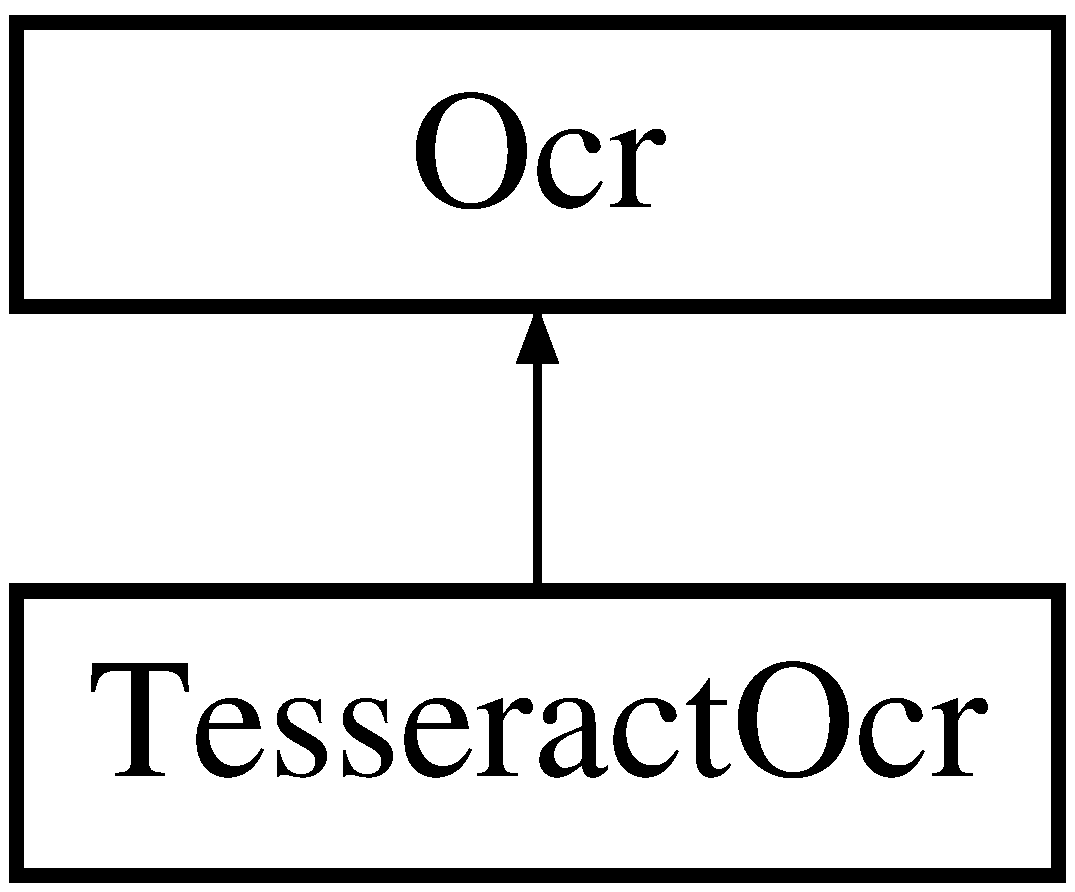
\includegraphics[height=2.000000cm]{classTesseractOcr}
\end{center}
\end{figure}
\subsection*{Public Member Functions}
\begin{DoxyCompactItemize}
\item 
\mbox{\hyperlink{classTesseractOcr_a9e62c15a4f8e4c8a0a614cf04ec8dea6}{Tesseract\+Ocr}} ()
\begin{DoxyCompactList}\small\item\em Creates an empty \mbox{\hyperlink{classTesseractOcr}{Tesseract\+Ocr}} instance. \end{DoxyCompactList}\item 
\mbox{\hyperlink{classTesseractOcr_ad550fd8468a1b1ee0b915c7202281dc7}{Tesseract\+Ocr}} (Q\+String image, Q\+String datapath=Q\+Dir(\char`\"{}../tesseract/tessdata\char`\"{}).absolute\+Path()+\textquotesingle{}/\textquotesingle{}, tesseract\+::\+Ocr\+Engine\+Mode engine\+Mode=tesseract\+::\+O\+E\+M\+\_\+\+T\+E\+S\+S\+E\+R\+A\+C\+T\+\_\+\+L\+S\+T\+M\+\_\+\+C\+O\+M\+B\+I\+N\+ED, tesseract\+::\+Page\+Seg\+Mode page\+Seg\+Mode=tesseract\+::\+P\+S\+M\+\_\+\+A\+U\+TO)
\begin{DoxyCompactList}\small\item\em Creates a \mbox{\hyperlink{classTesseractOcr}{Tesseract\+Ocr}} instante with the values received by parameter. \end{DoxyCompactList}\item 
\mbox{\hyperlink{classTesseractOcr_a8cac9f702b0eb765b522375d4aae08e9}{Tesseract\+Ocr}} (const \mbox{\hyperlink{classTesseractOcr}{Tesseract\+Ocr}} \&other)
\begin{DoxyCompactList}\small\item\em Creates a copy from other \mbox{\hyperlink{classTesseractOcr}{Tesseract\+Ocr}} instance. \end{DoxyCompactList}\item 
\mbox{\Hypertarget{classTesseractOcr_ad7d20b699dec0f1939c58eb0cc952406}\label{classTesseractOcr_ad7d20b699dec0f1939c58eb0cc952406}} 
\mbox{\hyperlink{classTesseractOcr_ad7d20b699dec0f1939c58eb0cc952406}{$\sim$\+Tesseract\+Ocr}} ()
\begin{DoxyCompactList}\small\item\em Destroys the tesseract ocr instance. \end{DoxyCompactList}\item 
Q\+String\+List \mbox{\hyperlink{classTesseractOcr_a7e5a1d3e275f710ce187bc1c0b080327}{extract}} () override
\begin{DoxyCompactList}\small\item\em Extracts strings contained in the image. \end{DoxyCompactList}\item 
Q\+String\+List \mbox{\hyperlink{classTesseractOcr_ad3486dcaa8a478c72ebaf76c43671326}{get\+Available\+Languages}} () const override
\begin{DoxyCompactList}\small\item\em Returns all available languages that can be used to extract strings from image. \end{DoxyCompactList}\item 
bool \mbox{\hyperlink{classTesseractOcr_aefe201ace3b144cb8834931b57f79bfd}{is\+Available\+Language}} (const Q\+String \&language) override
\begin{DoxyCompactList}\small\item\em Returns true if the language received by parameter is available to be used in the recognition, otherwise, returns false. \end{DoxyCompactList}\item 
tesseract\+::\+Page\+Seg\+Mode \mbox{\hyperlink{classTesseractOcr_afd6329838570d29a97834f3c91f0bb2c}{get\+Page\+Seg\+Mode}} () const
\begin{DoxyCompactList}\small\item\em Returns the page segmentation mode configured to be used. \end{DoxyCompactList}\item 
void \mbox{\hyperlink{classTesseractOcr_a16b1a94b0829a668e2f3ebc48c6e9e37}{set\+Page\+Seg\+Mode}} (tesseract\+::\+Page\+Seg\+Mode page\+Seg\+Mode)
\begin{DoxyCompactList}\small\item\em Sets the page segmentation mode to be used in the extraction. \end{DoxyCompactList}\item 
tesseract\+::\+Ocr\+Engine\+Mode \mbox{\hyperlink{classTesseractOcr_a911234ba57781e4e33515e2f0eab4320}{get\+Engine\+Mode}} () const
\begin{DoxyCompactList}\small\item\em Returns the engine mode configured to be used. \end{DoxyCompactList}\item 
void \mbox{\hyperlink{classTesseractOcr_acd714224045f4808b732f865164e1e1a}{set\+Engine\+Mode}} (tesseract\+::\+Ocr\+Engine\+Mode engine\+Mode)
\begin{DoxyCompactList}\small\item\em Sets the engine mode to be used in the extraction. \end{DoxyCompactList}\item 
\mbox{\hyperlink{classTesseractOcr}{Tesseract\+Ocr}} \& \mbox{\hyperlink{classTesseractOcr_ae1327017072b55801ce9ebdbab956b6a}{operator=}} (const \mbox{\hyperlink{classTesseractOcr}{Tesseract\+Ocr}} \&other)
\begin{DoxyCompactList}\small\item\em Assigns other to \mbox{\hyperlink{classTesseractOcr}{Tesseract\+Ocr}} and returns a reference to this \mbox{\hyperlink{classTesseractOcr}{Tesseract\+Ocr}} object. \end{DoxyCompactList}\end{DoxyCompactItemize}
\subsection*{Additional Inherited Members}


\subsection{Detailed Description}
This is a tool to detect string on images using tesseract api (\href{https://github.com/tesseract-ocr/tesseract}{\tt https\+://github.\+com/tesseract-\/ocr/tesseract}). 

Definition at line 21 of file tesseractocr.\+h.



\subsection{Constructor \& Destructor Documentation}
\mbox{\Hypertarget{classTesseractOcr_a9e62c15a4f8e4c8a0a614cf04ec8dea6}\label{classTesseractOcr_a9e62c15a4f8e4c8a0a614cf04ec8dea6}} 
\index{Tesseract\+Ocr@{Tesseract\+Ocr}!Tesseract\+Ocr@{Tesseract\+Ocr}}
\index{Tesseract\+Ocr@{Tesseract\+Ocr}!Tesseract\+Ocr@{Tesseract\+Ocr}}
\subsubsection{\texorpdfstring{Tesseract\+Ocr()}{TesseractOcr()}\hspace{0.1cm}{\footnotesize\ttfamily [1/3]}}
{\footnotesize\ttfamily Tesseract\+Ocr\+::\+Tesseract\+Ocr (\begin{DoxyParamCaption}{ }\end{DoxyParamCaption})}



Creates an empty \mbox{\hyperlink{classTesseractOcr}{Tesseract\+Ocr}} instance. 

Sets default values. 

Definition at line 14 of file tesseractocr.\+cpp.

\mbox{\Hypertarget{classTesseractOcr_ad550fd8468a1b1ee0b915c7202281dc7}\label{classTesseractOcr_ad550fd8468a1b1ee0b915c7202281dc7}} 
\index{Tesseract\+Ocr@{Tesseract\+Ocr}!Tesseract\+Ocr@{Tesseract\+Ocr}}
\index{Tesseract\+Ocr@{Tesseract\+Ocr}!Tesseract\+Ocr@{Tesseract\+Ocr}}
\subsubsection{\texorpdfstring{Tesseract\+Ocr()}{TesseractOcr()}\hspace{0.1cm}{\footnotesize\ttfamily [2/3]}}
{\footnotesize\ttfamily Tesseract\+Ocr\+::\+Tesseract\+Ocr (\begin{DoxyParamCaption}\item[{Q\+String}]{image,  }\item[{Q\+String}]{datapath = {\ttfamily QDir(\char`\"{}../tesseract/tessdata\char`\"{}).absolutePath()~+~\textquotesingle{}/\textquotesingle{}},  }\item[{tesseract\+::\+Ocr\+Engine\+Mode}]{engine\+Mode = {\ttfamily tesseract\+:\+:OEM\+\_\+TESSERACT\+\_\+LSTM\+\_\+COMBINED},  }\item[{tesseract\+::\+Page\+Seg\+Mode}]{page\+Seg\+Mode = {\ttfamily tesseract\+:\+:PSM\+\_\+AUTO} }\end{DoxyParamCaption})}



Creates a \mbox{\hyperlink{classTesseractOcr}{Tesseract\+Ocr}} instante with the values received by parameter. 


\begin{DoxyParams}{Parameters}
{\em image} & Path of image where strings will be ectracted. \\
\hline
{\em datapath} & Folder path where data languages will be. \\
\hline
{\em engine\+Mode} & Engine mode wich will use tesseract. \\
\hline
{\em page\+Seg\+Mode} & Page segmentation mode will use tesseract. \\
\hline
\end{DoxyParams}
$<$ Default language always \char`\"{}eng\char`\"{}.

$<$ Necessary for the api to work. 

Definition at line 19 of file tesseractocr.\+cpp.

\mbox{\Hypertarget{classTesseractOcr_a8cac9f702b0eb765b522375d4aae08e9}\label{classTesseractOcr_a8cac9f702b0eb765b522375d4aae08e9}} 
\index{Tesseract\+Ocr@{Tesseract\+Ocr}!Tesseract\+Ocr@{Tesseract\+Ocr}}
\index{Tesseract\+Ocr@{Tesseract\+Ocr}!Tesseract\+Ocr@{Tesseract\+Ocr}}
\subsubsection{\texorpdfstring{Tesseract\+Ocr()}{TesseractOcr()}\hspace{0.1cm}{\footnotesize\ttfamily [3/3]}}
{\footnotesize\ttfamily Tesseract\+Ocr\+::\+Tesseract\+Ocr (\begin{DoxyParamCaption}\item[{const \mbox{\hyperlink{classTesseractOcr}{Tesseract\+Ocr}} \&}]{other }\end{DoxyParamCaption})}



Creates a copy from other \mbox{\hyperlink{classTesseractOcr}{Tesseract\+Ocr}} instance. 


\begin{DoxyParams}{Parameters}
{\em other} & \\
\hline
\end{DoxyParams}
$<$ Necessary for the api to work. 

Definition at line 35 of file tesseractocr.\+cpp.



\subsection{Member Function Documentation}
\mbox{\Hypertarget{classTesseractOcr_a7e5a1d3e275f710ce187bc1c0b080327}\label{classTesseractOcr_a7e5a1d3e275f710ce187bc1c0b080327}} 
\index{Tesseract\+Ocr@{Tesseract\+Ocr}!extract@{extract}}
\index{extract@{extract}!Tesseract\+Ocr@{Tesseract\+Ocr}}
\subsubsection{\texorpdfstring{extract()}{extract()}}
{\footnotesize\ttfamily Q\+String\+List Tesseract\+Ocr\+::extract (\begin{DoxyParamCaption}{ }\end{DoxyParamCaption})\hspace{0.3cm}{\ttfamily [override]}, {\ttfamily [virtual]}}



Extracts strings contained in the image. 

Returns a Q\+Strings\+List containing the strings detected in the image. \begin{DoxyReturn}{Returns}
Strings list with strings extracted. 
\end{DoxyReturn}


Implements \mbox{\hyperlink{classOcr_a09a27b3a1f579c41ebda05f2a2cf4fed}{Ocr}}.



Definition at line 53 of file tesseractocr.\+cpp.

\mbox{\Hypertarget{classTesseractOcr_ad3486dcaa8a478c72ebaf76c43671326}\label{classTesseractOcr_ad3486dcaa8a478c72ebaf76c43671326}} 
\index{Tesseract\+Ocr@{Tesseract\+Ocr}!get\+Available\+Languages@{get\+Available\+Languages}}
\index{get\+Available\+Languages@{get\+Available\+Languages}!Tesseract\+Ocr@{Tesseract\+Ocr}}
\subsubsection{\texorpdfstring{get\+Available\+Languages()}{getAvailableLanguages()}}
{\footnotesize\ttfamily Q\+String\+List Tesseract\+Ocr\+::get\+Available\+Languages (\begin{DoxyParamCaption}{ }\end{DoxyParamCaption}) const\hspace{0.3cm}{\ttfamily [override]}, {\ttfamily [virtual]}}



Returns all available languages that can be used to extract strings from image. 

\begin{DoxyReturn}{Returns}
List with all available languages. 
\end{DoxyReturn}


Implements \mbox{\hyperlink{classOcr_a1b0eed20f8e7f553401834849d044bd2}{Ocr}}.



Definition at line 125 of file tesseractocr.\+cpp.

\mbox{\Hypertarget{classTesseractOcr_a911234ba57781e4e33515e2f0eab4320}\label{classTesseractOcr_a911234ba57781e4e33515e2f0eab4320}} 
\index{Tesseract\+Ocr@{Tesseract\+Ocr}!get\+Engine\+Mode@{get\+Engine\+Mode}}
\index{get\+Engine\+Mode@{get\+Engine\+Mode}!Tesseract\+Ocr@{Tesseract\+Ocr}}
\subsubsection{\texorpdfstring{get\+Engine\+Mode()}{getEngineMode()}}
{\footnotesize\ttfamily tesseract\+::\+Ocr\+Engine\+Mode Tesseract\+Ocr\+::get\+Engine\+Mode (\begin{DoxyParamCaption}{ }\end{DoxyParamCaption}) const}



Returns the engine mode configured to be used. 

\begin{DoxyReturn}{Returns}

\end{DoxyReturn}


Definition at line 159 of file tesseractocr.\+cpp.

\mbox{\Hypertarget{classTesseractOcr_afd6329838570d29a97834f3c91f0bb2c}\label{classTesseractOcr_afd6329838570d29a97834f3c91f0bb2c}} 
\index{Tesseract\+Ocr@{Tesseract\+Ocr}!get\+Page\+Seg\+Mode@{get\+Page\+Seg\+Mode}}
\index{get\+Page\+Seg\+Mode@{get\+Page\+Seg\+Mode}!Tesseract\+Ocr@{Tesseract\+Ocr}}
\subsubsection{\texorpdfstring{get\+Page\+Seg\+Mode()}{getPageSegMode()}}
{\footnotesize\ttfamily tesseract\+::\+Page\+Seg\+Mode Tesseract\+Ocr\+::get\+Page\+Seg\+Mode (\begin{DoxyParamCaption}{ }\end{DoxyParamCaption}) const}



Returns the page segmentation mode configured to be used. 

\begin{DoxyReturn}{Returns}
Page segmentation mode. 
\end{DoxyReturn}


Definition at line 149 of file tesseractocr.\+cpp.

\mbox{\Hypertarget{classTesseractOcr_aefe201ace3b144cb8834931b57f79bfd}\label{classTesseractOcr_aefe201ace3b144cb8834931b57f79bfd}} 
\index{Tesseract\+Ocr@{Tesseract\+Ocr}!is\+Available\+Language@{is\+Available\+Language}}
\index{is\+Available\+Language@{is\+Available\+Language}!Tesseract\+Ocr@{Tesseract\+Ocr}}
\subsubsection{\texorpdfstring{is\+Available\+Language()}{isAvailableLanguage()}}
{\footnotesize\ttfamily bool Tesseract\+Ocr\+::is\+Available\+Language (\begin{DoxyParamCaption}\item[{const Q\+String \&}]{language }\end{DoxyParamCaption})\hspace{0.3cm}{\ttfamily [override]}, {\ttfamily [virtual]}}



Returns true if the language received by parameter is available to be used in the recognition, otherwise, returns false. 


\begin{DoxyParams}{Parameters}
{\em language} & \mbox{\hyperlink{classString}{String}} language to check. \\
\hline
\end{DoxyParams}
\begin{DoxyReturn}{Returns}
bool 
\end{DoxyReturn}


Reimplemented from \mbox{\hyperlink{classOcr_a0c9ebb9b531bdcd6789d4bf9cffb1d42}{Ocr}}.



Definition at line 144 of file tesseractocr.\+cpp.

\mbox{\Hypertarget{classTesseractOcr_ae1327017072b55801ce9ebdbab956b6a}\label{classTesseractOcr_ae1327017072b55801ce9ebdbab956b6a}} 
\index{Tesseract\+Ocr@{Tesseract\+Ocr}!operator=@{operator=}}
\index{operator=@{operator=}!Tesseract\+Ocr@{Tesseract\+Ocr}}
\subsubsection{\texorpdfstring{operator=()}{operator=()}}
{\footnotesize\ttfamily \mbox{\hyperlink{classTesseractOcr}{Tesseract\+Ocr}} \& Tesseract\+Ocr\+::operator= (\begin{DoxyParamCaption}\item[{const \mbox{\hyperlink{classTesseractOcr}{Tesseract\+Ocr}} \&}]{other }\end{DoxyParamCaption})}



Assigns other to \mbox{\hyperlink{classTesseractOcr}{Tesseract\+Ocr}} and returns a reference to this \mbox{\hyperlink{classTesseractOcr}{Tesseract\+Ocr}} object. 


\begin{DoxyParams}{Parameters}
{\em other} & \mbox{\hyperlink{classTesseractOcr}{Tesseract\+Ocr}} object to be copied. \\
\hline
\end{DoxyParams}
\begin{DoxyReturn}{Returns}
Reference to this \mbox{\hyperlink{classTesseractOcr}{Tesseract\+Ocr}} object. 
\end{DoxyReturn}


Definition at line 212 of file tesseractocr.\+cpp.

\mbox{\Hypertarget{classTesseractOcr_acd714224045f4808b732f865164e1e1a}\label{classTesseractOcr_acd714224045f4808b732f865164e1e1a}} 
\index{Tesseract\+Ocr@{Tesseract\+Ocr}!set\+Engine\+Mode@{set\+Engine\+Mode}}
\index{set\+Engine\+Mode@{set\+Engine\+Mode}!Tesseract\+Ocr@{Tesseract\+Ocr}}
\subsubsection{\texorpdfstring{set\+Engine\+Mode()}{setEngineMode()}}
{\footnotesize\ttfamily void Tesseract\+Ocr\+::set\+Engine\+Mode (\begin{DoxyParamCaption}\item[{tesseract\+::\+Ocr\+Engine\+Mode}]{engine\+Mode }\end{DoxyParamCaption})}



Sets the engine mode to be used in the extraction. 


\begin{DoxyParams}{Parameters}
{\em engine\+Mode} & Engine mode. \\
\hline
\end{DoxyParams}


Definition at line 164 of file tesseractocr.\+cpp.

\mbox{\Hypertarget{classTesseractOcr_a16b1a94b0829a668e2f3ebc48c6e9e37}\label{classTesseractOcr_a16b1a94b0829a668e2f3ebc48c6e9e37}} 
\index{Tesseract\+Ocr@{Tesseract\+Ocr}!set\+Page\+Seg\+Mode@{set\+Page\+Seg\+Mode}}
\index{set\+Page\+Seg\+Mode@{set\+Page\+Seg\+Mode}!Tesseract\+Ocr@{Tesseract\+Ocr}}
\subsubsection{\texorpdfstring{set\+Page\+Seg\+Mode()}{setPageSegMode()}}
{\footnotesize\ttfamily void Tesseract\+Ocr\+::set\+Page\+Seg\+Mode (\begin{DoxyParamCaption}\item[{tesseract\+::\+Page\+Seg\+Mode}]{page\+Seg\+Mode }\end{DoxyParamCaption})}



Sets the page segmentation mode to be used in the extraction. 


\begin{DoxyParams}{Parameters}
{\em page\+Seg\+Mode} & Page segmentation mode. \\
\hline
\end{DoxyParams}


Definition at line 154 of file tesseractocr.\+cpp.



The documentation for this class was generated from the following files\+:\begin{DoxyCompactItemize}
\item 
src/optical\+\_\+character\+\_\+recognition/\mbox{\hyperlink{tesseractocr_8h}{tesseractocr.\+h}}\item 
src/optical\+\_\+character\+\_\+recognition/\mbox{\hyperlink{tesseractocr_8cpp}{tesseractocr.\+cpp}}\end{DoxyCompactItemize}

\hypertarget{classUtils}{}\section{Utils Class Reference}
\label{classUtils}\index{Utils@{Utils}}


This is static class with a lot of different utilities.  




{\ttfamily \#include $<$utils.\+h$>$}

\subsection*{Public Types}
\begin{DoxyCompactItemize}
\item 
enum \mbox{\hyperlink{classUtils_a32d52b4a749614335d60c2c3969b8df2}{Text\+Modifier}} \{ \newline
\mbox{\hyperlink{classUtils_a32d52b4a749614335d60c2c3969b8df2a39f1a78939e1d4ce79bcc88d8f0d6a1f}{F\+G\+\_\+\+B\+L\+A\+CK}} = 30, 
\mbox{\hyperlink{classUtils_a32d52b4a749614335d60c2c3969b8df2aecba2732375982cddf19e735b12bf9dc}{F\+G\+\_\+\+R\+ED}} = 31, 
\mbox{\hyperlink{classUtils_a32d52b4a749614335d60c2c3969b8df2afa2e3860716ac053c70f6a89f5a47e45}{F\+G\+\_\+\+G\+R\+E\+EN}} = 32, 
\mbox{\hyperlink{classUtils_a32d52b4a749614335d60c2c3969b8df2aa72d90f0070ff5f60c1226c7eee4d76e}{F\+G\+\_\+\+Y\+E\+L\+L\+OW}} = 33, 
\newline
\mbox{\hyperlink{classUtils_a32d52b4a749614335d60c2c3969b8df2a238297e309e520bd2796c968314b37d4}{F\+G\+\_\+\+B\+L\+UE}} = 34, 
\mbox{\hyperlink{classUtils_a32d52b4a749614335d60c2c3969b8df2a9fb8bfe4dbdecd2dea8dcc13691b6bfe}{F\+G\+\_\+\+M\+A\+G\+E\+N\+TA}} = 35, 
\mbox{\hyperlink{classUtils_a32d52b4a749614335d60c2c3969b8df2a7496759502c74e2fb1b6b41e40d708da}{F\+G\+\_\+\+C\+Y\+AN}} = 36, 
\mbox{\hyperlink{classUtils_a32d52b4a749614335d60c2c3969b8df2a0773c8537cc757b3f91ef3f056fc8e01}{F\+G\+\_\+\+W\+H\+I\+TE}} = 37, 
\newline
\mbox{\hyperlink{classUtils_a32d52b4a749614335d60c2c3969b8df2ae53e180d7734261c1eeb6f5b8046ee24}{B\+G\+\_\+\+B\+L\+A\+CK}} = 40, 
\mbox{\hyperlink{classUtils_a32d52b4a749614335d60c2c3969b8df2ae42dc37bb30e3d6a339e31b8799a0cc8}{B\+G\+\_\+\+R\+ED}} = 41, 
\mbox{\hyperlink{classUtils_a32d52b4a749614335d60c2c3969b8df2a304cda86f4e91dd0f25fe5cc49fa386f}{B\+G\+\_\+\+G\+R\+E\+EN}} = 42, 
\mbox{\hyperlink{classUtils_a32d52b4a749614335d60c2c3969b8df2a605748c9069d2aa85ecfc1b18546e65e}{B\+G\+\_\+\+Y\+E\+L\+L\+OW}} = 43, 
\newline
\mbox{\hyperlink{classUtils_a32d52b4a749614335d60c2c3969b8df2a4b3dbf96f2aa0105ccaee7642a0b9c43}{B\+G\+\_\+\+B\+L\+UE}} = 44, 
\mbox{\hyperlink{classUtils_a32d52b4a749614335d60c2c3969b8df2ab40a0e2307f8eaf9045c3e7871a67c37}{B\+G\+\_\+\+M\+A\+G\+E\+N\+TA}} = 45, 
\mbox{\hyperlink{classUtils_a32d52b4a749614335d60c2c3969b8df2a98728a943fa0b495de3d0aafc6000943}{B\+G\+\_\+\+C\+Y\+AN}} = 46, 
\mbox{\hyperlink{classUtils_a32d52b4a749614335d60c2c3969b8df2a4294fd26d218c1fae6ac2d0fe0fb99a3}{B\+G\+\_\+\+W\+H\+I\+TE}} = 47, 
\newline
\mbox{\hyperlink{classUtils_a32d52b4a749614335d60c2c3969b8df2a12907a9ced1317d0c7ba02f2dbe0b6ec}{R\+E\+S\+ET}} = 0, 
\mbox{\hyperlink{classUtils_a32d52b4a749614335d60c2c3969b8df2a34a3c1317c33b3b51ada23abfb30d0c3}{B\+O\+LD}} = 1, 
\mbox{\hyperlink{classUtils_a32d52b4a749614335d60c2c3969b8df2a0cdd170af17e97c899264ba026990145}{U\+N\+D\+E\+R\+L\+NE}} = 4, 
\mbox{\hyperlink{classUtils_a32d52b4a749614335d60c2c3969b8df2a69b78b99d4b769427fc5bff4cd756353}{I\+N\+V\+E\+R\+SE}} = 7, 
\newline
\mbox{\hyperlink{classUtils_a32d52b4a749614335d60c2c3969b8df2a30a8134b5e0cce11651d7cefdda133f3}{B\+O\+L\+D\+\_\+\+O\+FF}} = 21, 
\mbox{\hyperlink{classUtils_a32d52b4a749614335d60c2c3969b8df2a175f014d51622f39f71f5a275e52ffa0}{U\+N\+D\+E\+R\+L\+I\+N\+E\+\_\+\+O\+FF}} = 24, 
\mbox{\hyperlink{classUtils_a32d52b4a749614335d60c2c3969b8df2acb9181d52a5eaa0e2f557896d42f4139}{I\+N\+V\+E\+R\+S\+E\+\_\+\+O\+FF}} = 27
 \}
\end{DoxyCompactItemize}
\subsection*{Public Member Functions}
\begin{DoxyCompactItemize}
\item 
\mbox{\Hypertarget{classUtils_a452e78692c87ed5c7c993b6c6ac4981a}\label{classUtils_a452e78692c87ed5c7c993b6c6ac4981a}} 
\mbox{\hyperlink{classUtils_a452e78692c87ed5c7c993b6c6ac4981a}{Utils}} ()
\begin{DoxyCompactList}\small\item\em Creates an empty \mbox{\hyperlink{classUtils}{Utils}} object. \end{DoxyCompactList}\end{DoxyCompactItemize}
\subsection*{Static Public Member Functions}
\begin{DoxyCompactItemize}
\item 
static void \mbox{\hyperlink{classUtils_ac24a694013a7415b517f63a0641a0fb6}{error\+Message}} (const Q\+String \&text, const Q\+String \&informative\+Text)
\begin{DoxyCompactList}\small\item\em Creates a dialog and displayed it as a modal dialog. The dialog shown is an error dialog. \end{DoxyCompactList}\item 
static int \mbox{\hyperlink{classUtils_a3ff1c4308ffae59e9cc2bec504a1448a}{warning\+Message}} (const Q\+String \&text, const Q\+String \&informative\+Text)
\begin{DoxyCompactList}\small\item\em Creates a dialog and displayed it as a modal dialog. The dialog is a warning dialog. and only has to possible responses\+: Yes or No. \end{DoxyCompactList}\item 
static void \mbox{\hyperlink{classUtils_aeb00036fda3bd7faa92e805579fffa3e}{informative\+Message}} (const Q\+String \&text, const Q\+String \&informative\+Text)
\begin{DoxyCompactList}\small\item\em Creates a dialog and displayed it as a modal dialog. The dialog shown is an informative dialog. \end{DoxyCompactList}\item 
static bool \mbox{\hyperlink{classUtils_a77efde99fa16c21245f66273c7fded3a}{append\+File}} (const Q\+String \&path, const Q\+String \&text)
\begin{DoxyCompactList}\small\item\em Appends a text on a file. \end{DoxyCompactList}\item 
static bool \mbox{\hyperlink{classUtils_ae41ebd024526737fbaaada06e229b3c5}{write\+File}} (const Q\+String \&path, const Q\+String \&text)
\begin{DoxyCompactList}\small\item\em Write a text on a file. \end{DoxyCompactList}\item 
static Q\+Byte\+Array \mbox{\hyperlink{classUtils_a8ab4445ab51c372f969d3088ef0b73d9}{read\+All\+File}} (const Q\+String \&path)
\begin{DoxyCompactList}\small\item\em Read completely the file received by parameter. \end{DoxyCompactList}\item 
static int \mbox{\hyperlink{classUtils_a0ba873605d1b72ee448c18507d898d21}{execute\+Program}} (const Q\+String \&program, const Q\+String\+List \&arguments=Q\+String\+List(), const Q\+String \&standard\+Output=Q\+Process\+::null\+Device(), const Q\+String \&working\+Directory=Q\+String(), const int timeout=-\/1)
\begin{DoxyCompactList}\small\item\em Executes binary program. \end{DoxyCompactList}\item 
static Q\+String \mbox{\hyperlink{classUtils_ad33c4bda97a81483e4b34e692e747d0b}{zip\+Compress\+Directory\+Contents}} (const Q\+String \&directory, const Q\+String \&zip\+Destination, const Q\+String \&zip\+Name=\char`\"{}compressed\char`\"{})
\begin{DoxyCompactList}\small\item\em Compresses all files and folders in the directory received by argument. \end{DoxyCompactList}\item 
static Q\+Future$<$ void $>$ \mbox{\hyperlink{classUtils_a12f3c653e90f7ed38287f0a8897f60d5}{start\+Progress\+Dialog\+Counter}} (Q\+Progress\+Dialog $\ast$dialog, bool $\ast$has\+Finished, int timeout=40)
\begin{DoxyCompactList}\small\item\em Simulates a progress on a Q\+Progress\+Dialog. \end{DoxyCompactList}\item 
static bool \mbox{\hyperlink{classUtils_a1909e9cbf006b2ea0681d7c32605aca6}{is\+Valid\+Ip}} (const Q\+String \&ip)
\begin{DoxyCompactList}\small\item\em Returns true if is a valid ip, otherwise returns false. \end{DoxyCompactList}\item 
static Q\+String \mbox{\hyperlink{classUtils_aedd4143ac5a4b343d1486b9629a2d185}{get\+Date\+Time}} (Q\+String format=\char`\"{}yyyy\+\_\+\+M\+M\+\_\+dd\+\_\+hh\+\_\+mm\+\_\+ss\char`\"{})
\begin{DoxyCompactList}\small\item\em Returns a current date time with the format received by parameter. \end{DoxyCompactList}\item 
static Q\+String \mbox{\hyperlink{classUtils_a85a0cb065fa4399c42ce834952420d7a}{get\+Tmp\+Directory}} ()
\begin{DoxyCompactList}\small\item\em Returns a temporal directory of system. \end{DoxyCompactList}\item 
static Q\+String \mbox{\hyperlink{classUtils_a9885ad8eac3df9b5e22363dd1e9ff5b2}{format\+Text}} (const Q\+String \&text, Q\+List$<$ \mbox{\hyperlink{classUtils_a32d52b4a749614335d60c2c3969b8df2}{Text\+Modifier}} $>$ modifiers)
\begin{DoxyCompactList}\small\item\em Returns a text applying mofifiers to be used in terminal. \end{DoxyCompactList}\end{DoxyCompactItemize}


\subsection{Detailed Description}
This is static class with a lot of different utilities. 

Definition at line 25 of file utils.\+h.



\subsection{Member Enumeration Documentation}
\mbox{\Hypertarget{classUtils_a32d52b4a749614335d60c2c3969b8df2}\label{classUtils_a32d52b4a749614335d60c2c3969b8df2}} 
\index{Utils@{Utils}!Text\+Modifier@{Text\+Modifier}}
\index{Text\+Modifier@{Text\+Modifier}!Utils@{Utils}}
\subsubsection{\texorpdfstring{Text\+Modifier}{TextModifier}}
{\footnotesize\ttfamily enum \mbox{\hyperlink{classUtils_a32d52b4a749614335d60c2c3969b8df2}{Utils\+::\+Text\+Modifier}}}

\begin{DoxyEnumFields}{Enumerator}
\raisebox{\heightof{T}}[0pt][0pt]{\index{F\+G\+\_\+\+B\+L\+A\+CK@{F\+G\+\_\+\+B\+L\+A\+CK}!Utils@{Utils}}\index{Utils@{Utils}!F\+G\+\_\+\+B\+L\+A\+CK@{F\+G\+\_\+\+B\+L\+A\+CK}}}\mbox{\Hypertarget{classUtils_a32d52b4a749614335d60c2c3969b8df2a39f1a78939e1d4ce79bcc88d8f0d6a1f}\label{classUtils_a32d52b4a749614335d60c2c3969b8df2a39f1a78939e1d4ce79bcc88d8f0d6a1f}} 
F\+G\+\_\+\+B\+L\+A\+CK&Black foreground. \\
\hline

\raisebox{\heightof{T}}[0pt][0pt]{\index{F\+G\+\_\+\+R\+ED@{F\+G\+\_\+\+R\+ED}!Utils@{Utils}}\index{Utils@{Utils}!F\+G\+\_\+\+R\+ED@{F\+G\+\_\+\+R\+ED}}}\mbox{\Hypertarget{classUtils_a32d52b4a749614335d60c2c3969b8df2aecba2732375982cddf19e735b12bf9dc}\label{classUtils_a32d52b4a749614335d60c2c3969b8df2aecba2732375982cddf19e735b12bf9dc}} 
F\+G\+\_\+\+R\+ED&Red foreground. \\
\hline

\raisebox{\heightof{T}}[0pt][0pt]{\index{F\+G\+\_\+\+G\+R\+E\+EN@{F\+G\+\_\+\+G\+R\+E\+EN}!Utils@{Utils}}\index{Utils@{Utils}!F\+G\+\_\+\+G\+R\+E\+EN@{F\+G\+\_\+\+G\+R\+E\+EN}}}\mbox{\Hypertarget{classUtils_a32d52b4a749614335d60c2c3969b8df2afa2e3860716ac053c70f6a89f5a47e45}\label{classUtils_a32d52b4a749614335d60c2c3969b8df2afa2e3860716ac053c70f6a89f5a47e45}} 
F\+G\+\_\+\+G\+R\+E\+EN&Green foreground. \\
\hline

\raisebox{\heightof{T}}[0pt][0pt]{\index{F\+G\+\_\+\+Y\+E\+L\+L\+OW@{F\+G\+\_\+\+Y\+E\+L\+L\+OW}!Utils@{Utils}}\index{Utils@{Utils}!F\+G\+\_\+\+Y\+E\+L\+L\+OW@{F\+G\+\_\+\+Y\+E\+L\+L\+OW}}}\mbox{\Hypertarget{classUtils_a32d52b4a749614335d60c2c3969b8df2aa72d90f0070ff5f60c1226c7eee4d76e}\label{classUtils_a32d52b4a749614335d60c2c3969b8df2aa72d90f0070ff5f60c1226c7eee4d76e}} 
F\+G\+\_\+\+Y\+E\+L\+L\+OW&Yellow foreground. \\
\hline

\raisebox{\heightof{T}}[0pt][0pt]{\index{F\+G\+\_\+\+B\+L\+UE@{F\+G\+\_\+\+B\+L\+UE}!Utils@{Utils}}\index{Utils@{Utils}!F\+G\+\_\+\+B\+L\+UE@{F\+G\+\_\+\+B\+L\+UE}}}\mbox{\Hypertarget{classUtils_a32d52b4a749614335d60c2c3969b8df2a238297e309e520bd2796c968314b37d4}\label{classUtils_a32d52b4a749614335d60c2c3969b8df2a238297e309e520bd2796c968314b37d4}} 
F\+G\+\_\+\+B\+L\+UE&Blue foreground. \\
\hline

\raisebox{\heightof{T}}[0pt][0pt]{\index{F\+G\+\_\+\+M\+A\+G\+E\+N\+TA@{F\+G\+\_\+\+M\+A\+G\+E\+N\+TA}!Utils@{Utils}}\index{Utils@{Utils}!F\+G\+\_\+\+M\+A\+G\+E\+N\+TA@{F\+G\+\_\+\+M\+A\+G\+E\+N\+TA}}}\mbox{\Hypertarget{classUtils_a32d52b4a749614335d60c2c3969b8df2a9fb8bfe4dbdecd2dea8dcc13691b6bfe}\label{classUtils_a32d52b4a749614335d60c2c3969b8df2a9fb8bfe4dbdecd2dea8dcc13691b6bfe}} 
F\+G\+\_\+\+M\+A\+G\+E\+N\+TA&Magenta foreground. \\
\hline

\raisebox{\heightof{T}}[0pt][0pt]{\index{F\+G\+\_\+\+C\+Y\+AN@{F\+G\+\_\+\+C\+Y\+AN}!Utils@{Utils}}\index{Utils@{Utils}!F\+G\+\_\+\+C\+Y\+AN@{F\+G\+\_\+\+C\+Y\+AN}}}\mbox{\Hypertarget{classUtils_a32d52b4a749614335d60c2c3969b8df2a7496759502c74e2fb1b6b41e40d708da}\label{classUtils_a32d52b4a749614335d60c2c3969b8df2a7496759502c74e2fb1b6b41e40d708da}} 
F\+G\+\_\+\+C\+Y\+AN&Cyan foreground. \\
\hline

\raisebox{\heightof{T}}[0pt][0pt]{\index{F\+G\+\_\+\+W\+H\+I\+TE@{F\+G\+\_\+\+W\+H\+I\+TE}!Utils@{Utils}}\index{Utils@{Utils}!F\+G\+\_\+\+W\+H\+I\+TE@{F\+G\+\_\+\+W\+H\+I\+TE}}}\mbox{\Hypertarget{classUtils_a32d52b4a749614335d60c2c3969b8df2a0773c8537cc757b3f91ef3f056fc8e01}\label{classUtils_a32d52b4a749614335d60c2c3969b8df2a0773c8537cc757b3f91ef3f056fc8e01}} 
F\+G\+\_\+\+W\+H\+I\+TE&White foreground. \\
\hline

\raisebox{\heightof{T}}[0pt][0pt]{\index{B\+G\+\_\+\+B\+L\+A\+CK@{B\+G\+\_\+\+B\+L\+A\+CK}!Utils@{Utils}}\index{Utils@{Utils}!B\+G\+\_\+\+B\+L\+A\+CK@{B\+G\+\_\+\+B\+L\+A\+CK}}}\mbox{\Hypertarget{classUtils_a32d52b4a749614335d60c2c3969b8df2ae53e180d7734261c1eeb6f5b8046ee24}\label{classUtils_a32d52b4a749614335d60c2c3969b8df2ae53e180d7734261c1eeb6f5b8046ee24}} 
B\+G\+\_\+\+B\+L\+A\+CK&Black background. \\
\hline

\raisebox{\heightof{T}}[0pt][0pt]{\index{B\+G\+\_\+\+R\+ED@{B\+G\+\_\+\+R\+ED}!Utils@{Utils}}\index{Utils@{Utils}!B\+G\+\_\+\+R\+ED@{B\+G\+\_\+\+R\+ED}}}\mbox{\Hypertarget{classUtils_a32d52b4a749614335d60c2c3969b8df2ae42dc37bb30e3d6a339e31b8799a0cc8}\label{classUtils_a32d52b4a749614335d60c2c3969b8df2ae42dc37bb30e3d6a339e31b8799a0cc8}} 
B\+G\+\_\+\+R\+ED&Red background. \\
\hline

\raisebox{\heightof{T}}[0pt][0pt]{\index{B\+G\+\_\+\+G\+R\+E\+EN@{B\+G\+\_\+\+G\+R\+E\+EN}!Utils@{Utils}}\index{Utils@{Utils}!B\+G\+\_\+\+G\+R\+E\+EN@{B\+G\+\_\+\+G\+R\+E\+EN}}}\mbox{\Hypertarget{classUtils_a32d52b4a749614335d60c2c3969b8df2a304cda86f4e91dd0f25fe5cc49fa386f}\label{classUtils_a32d52b4a749614335d60c2c3969b8df2a304cda86f4e91dd0f25fe5cc49fa386f}} 
B\+G\+\_\+\+G\+R\+E\+EN&Green background. \\
\hline

\raisebox{\heightof{T}}[0pt][0pt]{\index{B\+G\+\_\+\+Y\+E\+L\+L\+OW@{B\+G\+\_\+\+Y\+E\+L\+L\+OW}!Utils@{Utils}}\index{Utils@{Utils}!B\+G\+\_\+\+Y\+E\+L\+L\+OW@{B\+G\+\_\+\+Y\+E\+L\+L\+OW}}}\mbox{\Hypertarget{classUtils_a32d52b4a749614335d60c2c3969b8df2a605748c9069d2aa85ecfc1b18546e65e}\label{classUtils_a32d52b4a749614335d60c2c3969b8df2a605748c9069d2aa85ecfc1b18546e65e}} 
B\+G\+\_\+\+Y\+E\+L\+L\+OW&Yellow background. \\
\hline

\raisebox{\heightof{T}}[0pt][0pt]{\index{B\+G\+\_\+\+B\+L\+UE@{B\+G\+\_\+\+B\+L\+UE}!Utils@{Utils}}\index{Utils@{Utils}!B\+G\+\_\+\+B\+L\+UE@{B\+G\+\_\+\+B\+L\+UE}}}\mbox{\Hypertarget{classUtils_a32d52b4a749614335d60c2c3969b8df2a4b3dbf96f2aa0105ccaee7642a0b9c43}\label{classUtils_a32d52b4a749614335d60c2c3969b8df2a4b3dbf96f2aa0105ccaee7642a0b9c43}} 
B\+G\+\_\+\+B\+L\+UE&Blue background. \\
\hline

\raisebox{\heightof{T}}[0pt][0pt]{\index{B\+G\+\_\+\+M\+A\+G\+E\+N\+TA@{B\+G\+\_\+\+M\+A\+G\+E\+N\+TA}!Utils@{Utils}}\index{Utils@{Utils}!B\+G\+\_\+\+M\+A\+G\+E\+N\+TA@{B\+G\+\_\+\+M\+A\+G\+E\+N\+TA}}}\mbox{\Hypertarget{classUtils_a32d52b4a749614335d60c2c3969b8df2ab40a0e2307f8eaf9045c3e7871a67c37}\label{classUtils_a32d52b4a749614335d60c2c3969b8df2ab40a0e2307f8eaf9045c3e7871a67c37}} 
B\+G\+\_\+\+M\+A\+G\+E\+N\+TA&Magenta background. \\
\hline

\raisebox{\heightof{T}}[0pt][0pt]{\index{B\+G\+\_\+\+C\+Y\+AN@{B\+G\+\_\+\+C\+Y\+AN}!Utils@{Utils}}\index{Utils@{Utils}!B\+G\+\_\+\+C\+Y\+AN@{B\+G\+\_\+\+C\+Y\+AN}}}\mbox{\Hypertarget{classUtils_a32d52b4a749614335d60c2c3969b8df2a98728a943fa0b495de3d0aafc6000943}\label{classUtils_a32d52b4a749614335d60c2c3969b8df2a98728a943fa0b495de3d0aafc6000943}} 
B\+G\+\_\+\+C\+Y\+AN&Cyan background. \\
\hline

\raisebox{\heightof{T}}[0pt][0pt]{\index{B\+G\+\_\+\+W\+H\+I\+TE@{B\+G\+\_\+\+W\+H\+I\+TE}!Utils@{Utils}}\index{Utils@{Utils}!B\+G\+\_\+\+W\+H\+I\+TE@{B\+G\+\_\+\+W\+H\+I\+TE}}}\mbox{\Hypertarget{classUtils_a32d52b4a749614335d60c2c3969b8df2a4294fd26d218c1fae6ac2d0fe0fb99a3}\label{classUtils_a32d52b4a749614335d60c2c3969b8df2a4294fd26d218c1fae6ac2d0fe0fb99a3}} 
B\+G\+\_\+\+W\+H\+I\+TE&White background. \\
\hline

\raisebox{\heightof{T}}[0pt][0pt]{\index{R\+E\+S\+ET@{R\+E\+S\+ET}!Utils@{Utils}}\index{Utils@{Utils}!R\+E\+S\+ET@{R\+E\+S\+ET}}}\mbox{\Hypertarget{classUtils_a32d52b4a749614335d60c2c3969b8df2a12907a9ced1317d0c7ba02f2dbe0b6ec}\label{classUtils_a32d52b4a749614335d60c2c3969b8df2a12907a9ced1317d0c7ba02f2dbe0b6ec}} 
R\+E\+S\+ET&Reset all. \\
\hline

\raisebox{\heightof{T}}[0pt][0pt]{\index{B\+O\+LD@{B\+O\+LD}!Utils@{Utils}}\index{Utils@{Utils}!B\+O\+LD@{B\+O\+LD}}}\mbox{\Hypertarget{classUtils_a32d52b4a749614335d60c2c3969b8df2a34a3c1317c33b3b51ada23abfb30d0c3}\label{classUtils_a32d52b4a749614335d60c2c3969b8df2a34a3c1317c33b3b51ada23abfb30d0c3}} 
B\+O\+LD&Bold text. \\
\hline

\raisebox{\heightof{T}}[0pt][0pt]{\index{U\+N\+D\+E\+R\+L\+NE@{U\+N\+D\+E\+R\+L\+NE}!Utils@{Utils}}\index{Utils@{Utils}!U\+N\+D\+E\+R\+L\+NE@{U\+N\+D\+E\+R\+L\+NE}}}\mbox{\Hypertarget{classUtils_a32d52b4a749614335d60c2c3969b8df2a0cdd170af17e97c899264ba026990145}\label{classUtils_a32d52b4a749614335d60c2c3969b8df2a0cdd170af17e97c899264ba026990145}} 
U\+N\+D\+E\+R\+L\+NE&Underline text. \\
\hline

\raisebox{\heightof{T}}[0pt][0pt]{\index{I\+N\+V\+E\+R\+SE@{I\+N\+V\+E\+R\+SE}!Utils@{Utils}}\index{Utils@{Utils}!I\+N\+V\+E\+R\+SE@{I\+N\+V\+E\+R\+SE}}}\mbox{\Hypertarget{classUtils_a32d52b4a749614335d60c2c3969b8df2a69b78b99d4b769427fc5bff4cd756353}\label{classUtils_a32d52b4a749614335d60c2c3969b8df2a69b78b99d4b769427fc5bff4cd756353}} 
I\+N\+V\+E\+R\+SE&Inverse text. \\
\hline

\raisebox{\heightof{T}}[0pt][0pt]{\index{B\+O\+L\+D\+\_\+\+O\+FF@{B\+O\+L\+D\+\_\+\+O\+FF}!Utils@{Utils}}\index{Utils@{Utils}!B\+O\+L\+D\+\_\+\+O\+FF@{B\+O\+L\+D\+\_\+\+O\+FF}}}\mbox{\Hypertarget{classUtils_a32d52b4a749614335d60c2c3969b8df2a30a8134b5e0cce11651d7cefdda133f3}\label{classUtils_a32d52b4a749614335d60c2c3969b8df2a30a8134b5e0cce11651d7cefdda133f3}} 
B\+O\+L\+D\+\_\+\+O\+FF&Off bold text. \\
\hline

\raisebox{\heightof{T}}[0pt][0pt]{\index{U\+N\+D\+E\+R\+L\+I\+N\+E\+\_\+\+O\+FF@{U\+N\+D\+E\+R\+L\+I\+N\+E\+\_\+\+O\+FF}!Utils@{Utils}}\index{Utils@{Utils}!U\+N\+D\+E\+R\+L\+I\+N\+E\+\_\+\+O\+FF@{U\+N\+D\+E\+R\+L\+I\+N\+E\+\_\+\+O\+FF}}}\mbox{\Hypertarget{classUtils_a32d52b4a749614335d60c2c3969b8df2a175f014d51622f39f71f5a275e52ffa0}\label{classUtils_a32d52b4a749614335d60c2c3969b8df2a175f014d51622f39f71f5a275e52ffa0}} 
U\+N\+D\+E\+R\+L\+I\+N\+E\+\_\+\+O\+FF&Off underline text. \\
\hline

\raisebox{\heightof{T}}[0pt][0pt]{\index{I\+N\+V\+E\+R\+S\+E\+\_\+\+O\+FF@{I\+N\+V\+E\+R\+S\+E\+\_\+\+O\+FF}!Utils@{Utils}}\index{Utils@{Utils}!I\+N\+V\+E\+R\+S\+E\+\_\+\+O\+FF@{I\+N\+V\+E\+R\+S\+E\+\_\+\+O\+FF}}}\mbox{\Hypertarget{classUtils_a32d52b4a749614335d60c2c3969b8df2acb9181d52a5eaa0e2f557896d42f4139}\label{classUtils_a32d52b4a749614335d60c2c3969b8df2acb9181d52a5eaa0e2f557896d42f4139}} 
I\+N\+V\+E\+R\+S\+E\+\_\+\+O\+FF&Off inverse text. \\
\hline

\end{DoxyEnumFields}


Definition at line 28 of file utils.\+h.



\subsection{Member Function Documentation}
\mbox{\Hypertarget{classUtils_a77efde99fa16c21245f66273c7fded3a}\label{classUtils_a77efde99fa16c21245f66273c7fded3a}} 
\index{Utils@{Utils}!append\+File@{append\+File}}
\index{append\+File@{append\+File}!Utils@{Utils}}
\subsubsection{\texorpdfstring{append\+File()}{appendFile()}}
{\footnotesize\ttfamily bool Utils\+::append\+File (\begin{DoxyParamCaption}\item[{const Q\+String \&}]{path,  }\item[{const Q\+String \&}]{text }\end{DoxyParamCaption})\hspace{0.3cm}{\ttfamily [static]}}



Appends a text on a file. 

If the file exists is not overwritten. If the file does not exist is created. Returns true if the text is added succesfully, otherwise returns false. 
\begin{DoxyParams}{Parameters}
{\em path} & File where will append the text. \\
\hline
{\em text} & Text to be appended on the file. \\
\hline
\end{DoxyParams}
\begin{DoxyReturn}{Returns}
bool 
\end{DoxyReturn}


Definition at line 63 of file utils.\+cpp.

\mbox{\Hypertarget{classUtils_ac24a694013a7415b517f63a0641a0fb6}\label{classUtils_ac24a694013a7415b517f63a0641a0fb6}} 
\index{Utils@{Utils}!error\+Message@{error\+Message}}
\index{error\+Message@{error\+Message}!Utils@{Utils}}
\subsubsection{\texorpdfstring{error\+Message()}{errorMessage()}}
{\footnotesize\ttfamily void Utils\+::error\+Message (\begin{DoxyParamCaption}\item[{const Q\+String \&}]{text,  }\item[{const Q\+String \&}]{informative\+Text }\end{DoxyParamCaption})\hspace{0.3cm}{\ttfamily [static]}}



Creates a dialog and displayed it as a modal dialog. The dialog shown is an error dialog. 

The user only can accept the dialog.

The function is designed to display error messages to the user without the option of choosing anything. 
\begin{DoxyParams}{Parameters}
{\em text} & Message text to be displayed. \\
\hline
{\em informative\+Text} & Informative text that provides a fuller description for the message. \\
\hline
\end{DoxyParams}


Definition at line 18 of file utils.\+cpp.

\mbox{\Hypertarget{classUtils_a0ba873605d1b72ee448c18507d898d21}\label{classUtils_a0ba873605d1b72ee448c18507d898d21}} 
\index{Utils@{Utils}!execute\+Program@{execute\+Program}}
\index{execute\+Program@{execute\+Program}!Utils@{Utils}}
\subsubsection{\texorpdfstring{execute\+Program()}{executeProgram()}}
{\footnotesize\ttfamily int Utils\+::execute\+Program (\begin{DoxyParamCaption}\item[{const Q\+String \&}]{program,  }\item[{const Q\+String\+List \&}]{arguments = {\ttfamily QStringList()},  }\item[{const Q\+String \&}]{standard\+Output = {\ttfamily QProcess\+:\+:nullDevice()},  }\item[{const Q\+String \&}]{working\+Directory = {\ttfamily QString()},  }\item[{const int}]{timeout = {\ttfamily -\/1} }\end{DoxyParamCaption})\hspace{0.3cm}{\ttfamily [static]}}



Executes binary program. 

Returns the code error returned by the execution.

If an empty standard output file is received, standard output is not saved.

If an empty working directory is received, the process is executed in current directory.

A timeout equals to -\/1 indicates that process has not limit time.

Some known code errors\+: -\/$>$ 255\+: binary file not found or can\textquotesingle{}t be executed. -\/$>$ -\/1\+: binary file crashed during the execution. 
\begin{DoxyParams}{Parameters}
{\em program} & Name of binary file. \\
\hline
{\em arguments} & Arguments of the program. \\
\hline
{\em standard\+Output} & File path where process standard output will be saved. \\
\hline
{\em work\+Directory} & Directory where the program must work. \\
\hline
{\em timeout} & Execution timeout of the program. \\
\hline
\end{DoxyParams}
\begin{DoxyReturn}{Returns}
Code error of the execution 
\end{DoxyReturn}


Definition at line 105 of file utils.\+cpp.

\mbox{\Hypertarget{classUtils_a9885ad8eac3df9b5e22363dd1e9ff5b2}\label{classUtils_a9885ad8eac3df9b5e22363dd1e9ff5b2}} 
\index{Utils@{Utils}!format\+Text@{format\+Text}}
\index{format\+Text@{format\+Text}!Utils@{Utils}}
\subsubsection{\texorpdfstring{format\+Text()}{formatText()}}
{\footnotesize\ttfamily Q\+String Utils\+::format\+Text (\begin{DoxyParamCaption}\item[{const Q\+String \&}]{text,  }\item[{Q\+List$<$ \mbox{\hyperlink{classUtils_a32d52b4a749614335d60c2c3969b8df2}{Text\+Modifier}} $>$}]{modifiers }\end{DoxyParamCaption})\hspace{0.3cm}{\ttfamily [static]}}



Returns a text applying mofifiers to be used in terminal. 

This function use A\+N\+SI format, make sure your terminal accepts it. 
\begin{DoxyParams}{Parameters}
{\em text} & \mbox{\hyperlink{classString}{String}} to be formatted. \\
\hline
{\em modifiers} & Modifiers to be applied \\
\hline
\end{DoxyParams}
\begin{DoxyReturn}{Returns}

\end{DoxyReturn}


Definition at line 187 of file utils.\+cpp.

\mbox{\Hypertarget{classUtils_aedd4143ac5a4b343d1486b9629a2d185}\label{classUtils_aedd4143ac5a4b343d1486b9629a2d185}} 
\index{Utils@{Utils}!get\+Date\+Time@{get\+Date\+Time}}
\index{get\+Date\+Time@{get\+Date\+Time}!Utils@{Utils}}
\subsubsection{\texorpdfstring{get\+Date\+Time()}{getDateTime()}}
{\footnotesize\ttfamily Q\+String Utils\+::get\+Date\+Time (\begin{DoxyParamCaption}\item[{Q\+String}]{format = {\ttfamily \char`\"{}yyyy\+\_\+MM\+\_\+dd\+\_\+hh\+\_\+mm\+\_\+ss\char`\"{}} }\end{DoxyParamCaption})\hspace{0.3cm}{\ttfamily [static]}}



Returns a current date time with the format received by parameter. 


\begin{DoxyParams}{Parameters}
{\em format} & Format to returns the date time. \\
\hline
\end{DoxyParams}
\begin{DoxyReturn}{Returns}
Date time. 
\end{DoxyReturn}


Definition at line 177 of file utils.\+cpp.

\mbox{\Hypertarget{classUtils_a85a0cb065fa4399c42ce834952420d7a}\label{classUtils_a85a0cb065fa4399c42ce834952420d7a}} 
\index{Utils@{Utils}!get\+Tmp\+Directory@{get\+Tmp\+Directory}}
\index{get\+Tmp\+Directory@{get\+Tmp\+Directory}!Utils@{Utils}}
\subsubsection{\texorpdfstring{get\+Tmp\+Directory()}{getTmpDirectory()}}
{\footnotesize\ttfamily Q\+String Utils\+::get\+Tmp\+Directory (\begin{DoxyParamCaption}{ }\end{DoxyParamCaption})\hspace{0.3cm}{\ttfamily [static]}}



Returns a temporal directory of system. 

\begin{DoxyReturn}{Returns}

\end{DoxyReturn}


Definition at line 182 of file utils.\+cpp.

\mbox{\Hypertarget{classUtils_aeb00036fda3bd7faa92e805579fffa3e}\label{classUtils_aeb00036fda3bd7faa92e805579fffa3e}} 
\index{Utils@{Utils}!informative\+Message@{informative\+Message}}
\index{informative\+Message@{informative\+Message}!Utils@{Utils}}
\subsubsection{\texorpdfstring{informative\+Message()}{informativeMessage()}}
{\footnotesize\ttfamily void Utils\+::informative\+Message (\begin{DoxyParamCaption}\item[{const Q\+String \&}]{text,  }\item[{const Q\+String \&}]{informative\+Text }\end{DoxyParamCaption})\hspace{0.3cm}{\ttfamily [static]}}



Creates a dialog and displayed it as a modal dialog. The dialog shown is an informative dialog. 

The user only can accept the dialog.

The function is designed to display informative messages to the user. 
\begin{DoxyParams}{Parameters}
{\em text} & Message text to be displayed. \\
\hline
{\em informative\+Text} & Informative text that provides a fuller description for the message. \\
\hline
\end{DoxyParams}


Definition at line 48 of file utils.\+cpp.

\mbox{\Hypertarget{classUtils_a1909e9cbf006b2ea0681d7c32605aca6}\label{classUtils_a1909e9cbf006b2ea0681d7c32605aca6}} 
\index{Utils@{Utils}!is\+Valid\+Ip@{is\+Valid\+Ip}}
\index{is\+Valid\+Ip@{is\+Valid\+Ip}!Utils@{Utils}}
\subsubsection{\texorpdfstring{is\+Valid\+Ip()}{isValidIp()}}
{\footnotesize\ttfamily bool Utils\+::is\+Valid\+Ip (\begin{DoxyParamCaption}\item[{const Q\+String \&}]{ip }\end{DoxyParamCaption})\hspace{0.3cm}{\ttfamily [static]}}



Returns true if is a valid ip, otherwise returns false. 


\begin{DoxyParams}{Parameters}
{\em ip} & Ip to be checked. \\
\hline
\end{DoxyParams}
\begin{DoxyReturn}{Returns}
bool 
\end{DoxyReturn}


Definition at line 169 of file utils.\+cpp.

\mbox{\Hypertarget{classUtils_a8ab4445ab51c372f969d3088ef0b73d9}\label{classUtils_a8ab4445ab51c372f969d3088ef0b73d9}} 
\index{Utils@{Utils}!read\+All\+File@{read\+All\+File}}
\index{read\+All\+File@{read\+All\+File}!Utils@{Utils}}
\subsubsection{\texorpdfstring{read\+All\+File()}{readAllFile()}}
{\footnotesize\ttfamily Q\+Byte\+Array Utils\+::read\+All\+File (\begin{DoxyParamCaption}\item[{const Q\+String \&}]{path }\end{DoxyParamCaption})\hspace{0.3cm}{\ttfamily [static]}}



Read completely the file received by parameter. 

Returns a Q\+Byte\+Array object with the data of the file or an empty Q\+Byte\+Array if something wrong. 
\begin{DoxyParams}{Parameters}
{\em path} & File to be read. \\
\hline
\end{DoxyParams}
\begin{DoxyReturn}{Returns}
Data read from the file. 
\end{DoxyReturn}


Definition at line 90 of file utils.\+cpp.

\mbox{\Hypertarget{classUtils_a12f3c653e90f7ed38287f0a8897f60d5}\label{classUtils_a12f3c653e90f7ed38287f0a8897f60d5}} 
\index{Utils@{Utils}!start\+Progress\+Dialog\+Counter@{start\+Progress\+Dialog\+Counter}}
\index{start\+Progress\+Dialog\+Counter@{start\+Progress\+Dialog\+Counter}!Utils@{Utils}}
\subsubsection{\texorpdfstring{start\+Progress\+Dialog\+Counter()}{startProgressDialogCounter()}}
{\footnotesize\ttfamily Q\+Future$<$ void $>$ Utils\+::start\+Progress\+Dialog\+Counter (\begin{DoxyParamCaption}\item[{Q\+Progress\+Dialog $\ast$}]{dialog,  }\item[{bool $\ast$}]{has\+Finished,  }\item[{int}]{timeout = {\ttfamily 40} }\end{DoxyParamCaption})\hspace{0.3cm}{\ttfamily [static]}}



Simulates a progress on a Q\+Progress\+Dialog. 

Counter only finish when has\+Finished is true, otherwise progress count stop in 99\%. As the counter is created in other thread, out of function you have to make sure that thread finished calling function Q\+Future\+::wait\+For\+Finished(). If you don\textquotesingle{}t make sure of it, your program probably will finish unexpectedly with an error.

Returns a Q\+Future object for control the end of the thread. 
\begin{DoxyParams}{Parameters}
{\em dialog} & Dialog where exec the counter. \\
\hline
{\em has\+Finished} & Flag to finish the counter. \\
\hline
{\em timeout} & Time between each increase in the percentage of progress. \\
\hline
\end{DoxyParams}
\begin{DoxyReturn}{Returns}
Q\+Future object to know when the thread has finished. 
\end{DoxyReturn}


Definition at line 145 of file utils.\+cpp.

\mbox{\Hypertarget{classUtils_a3ff1c4308ffae59e9cc2bec504a1448a}\label{classUtils_a3ff1c4308ffae59e9cc2bec504a1448a}} 
\index{Utils@{Utils}!warning\+Message@{warning\+Message}}
\index{warning\+Message@{warning\+Message}!Utils@{Utils}}
\subsubsection{\texorpdfstring{warning\+Message()}{warningMessage()}}
{\footnotesize\ttfamily int Utils\+::warning\+Message (\begin{DoxyParamCaption}\item[{const Q\+String \&}]{text,  }\item[{const Q\+String \&}]{informative\+Text }\end{DoxyParamCaption})\hspace{0.3cm}{\ttfamily [static]}}



Creates a dialog and displayed it as a modal dialog. The dialog is a warning dialog. and only has to possible responses\+: Yes or No. 

The dialog has only two buttons (Yes and No), which are the two possible options that the user can select. Returns the option selected by the user.

The function is designed to display warning messages to the user and whether he wants to take the risks. 
\begin{DoxyParams}{Parameters}
{\em text} & Message text to be displayed. \\
\hline
{\em informative\+Text} & Informative text that provides a fuller description for the message. \\
\hline
\end{DoxyParams}
\begin{DoxyReturn}{Returns}
User responser. 
\end{DoxyReturn}


Definition at line 33 of file utils.\+cpp.

\mbox{\Hypertarget{classUtils_ae41ebd024526737fbaaada06e229b3c5}\label{classUtils_ae41ebd024526737fbaaada06e229b3c5}} 
\index{Utils@{Utils}!write\+File@{write\+File}}
\index{write\+File@{write\+File}!Utils@{Utils}}
\subsubsection{\texorpdfstring{write\+File()}{writeFile()}}
{\footnotesize\ttfamily bool Utils\+::write\+File (\begin{DoxyParamCaption}\item[{const Q\+String \&}]{path,  }\item[{const Q\+String \&}]{text }\end{DoxyParamCaption})\hspace{0.3cm}{\ttfamily [static]}}



Write a text on a file. 

If the file exists is overwritten. If the file does not exist is created. Returns true if the text is written succesfully, otherwise returns false. 
\begin{DoxyParams}{Parameters}
{\em path} & File where will write the text. \\
\hline
{\em text} & Text to be wroten on the file. \\
\hline
\end{DoxyParams}
\begin{DoxyReturn}{Returns}
bool 
\end{DoxyReturn}


Definition at line 76 of file utils.\+cpp.

\mbox{\Hypertarget{classUtils_ad33c4bda97a81483e4b34e692e747d0b}\label{classUtils_ad33c4bda97a81483e4b34e692e747d0b}} 
\index{Utils@{Utils}!zip\+Compress\+Directory\+Contents@{zip\+Compress\+Directory\+Contents}}
\index{zip\+Compress\+Directory\+Contents@{zip\+Compress\+Directory\+Contents}!Utils@{Utils}}
\subsubsection{\texorpdfstring{zip\+Compress\+Directory\+Contents()}{zipCompressDirectoryContents()}}
{\footnotesize\ttfamily Q\+String Utils\+::zip\+Compress\+Directory\+Contents (\begin{DoxyParamCaption}\item[{const Q\+String \&}]{directory,  }\item[{const Q\+String \&}]{zip\+Destination,  }\item[{const Q\+String \&}]{zip\+Name = {\ttfamily \char`\"{}compressed\char`\"{}} }\end{DoxyParamCaption})\hspace{0.3cm}{\ttfamily [static]}}



Compresses all files and folders in the directory received by argument. 

If compressing was succesfull, returns the absolute path of the zip file. Otherwise returns an empty string. 
\begin{DoxyParams}{Parameters}
{\em directory} & Path of directory to be compressed. \\
\hline
{\em zip\+Destination} & Path where de zip file will be saved. \\
\hline
{\em zip\+Name} & Name to be setted to the file. \\
\hline
\end{DoxyParams}
\begin{DoxyReturn}{Returns}
Absolute path of the result zip file. 
\end{DoxyReturn}


Definition at line 131 of file utils.\+cpp.



The documentation for this class was generated from the following files\+:\begin{DoxyCompactItemize}
\item 
src/tools/\mbox{\hyperlink{utils_8h}{utils.\+h}}\item 
src/tools/\mbox{\hyperlink{utils_8cpp}{utils.\+cpp}}\end{DoxyCompactItemize}

\hypertarget{classWindowsConsoleController}{}\section{Windows\+Console\+Controller Class Reference}
\label{classWindowsConsoleController}\index{Windows\+Console\+Controller@{Windows\+Console\+Controller}}


This is the controller class that works a Windows C\+LI environment.  




{\ttfamily \#include $<$windowsconsolecontroller.\+h$>$}

Inheritance diagram for Windows\+Console\+Controller\+:\begin{figure}[H]
\begin{center}
\leavevmode
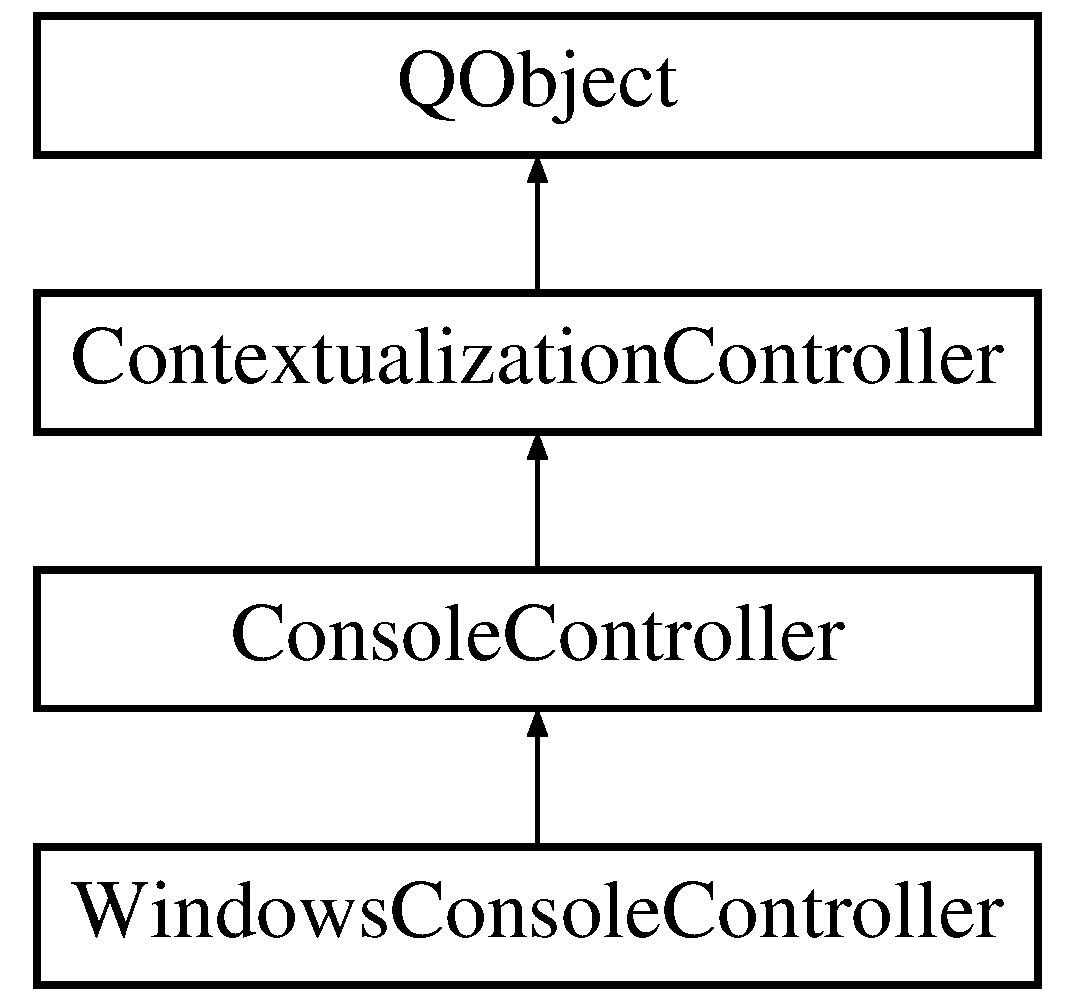
\includegraphics[height=4.000000cm]{classWindowsConsoleController}
\end{center}
\end{figure}
\subsection*{Public Member Functions}
\begin{DoxyCompactItemize}
\item 
\mbox{\Hypertarget{classWindowsConsoleController_ac2d015316b132fb43289d44277b33e3b}\label{classWindowsConsoleController_ac2d015316b132fb43289d44277b33e3b}} 
\mbox{\hyperlink{classWindowsConsoleController_ac2d015316b132fb43289d44277b33e3b}{Windows\+Console\+Controller}} ()
\begin{DoxyCompactList}\small\item\em Creates an empty \mbox{\hyperlink{classWindowsConsoleController}{Windows\+Console\+Controller}}. \end{DoxyCompactList}\item 
\mbox{\hyperlink{classWindowsConsoleController_a684161508236414615ee30bc9b29b79f}{Windows\+Console\+Controller}} (int argc, char $\ast$$\ast$argv)
\begin{DoxyCompactList}\small\item\em Creates a \mbox{\hyperlink{classWindowsConsoleController}{Windows\+Console\+Controller}} initialited with the parameter received in argv. \end{DoxyCompactList}\item 
Q\+String \mbox{\hyperlink{classWindowsConsoleController_ab536d94896c62a1920a6dbfd4b83c18b}{take\+Capture\+Area}} () override
\begin{DoxyCompactList}\small\item\em Starts a process that allow user capture an area of the screen. \end{DoxyCompactList}\item 
int \mbox{\hyperlink{classWindowsConsoleController_afca6af922fe103845177580d6af4859e}{generate\+Done\+Fp\+File}} () override
\begin{DoxyCompactList}\small\item\em Creates a copy of english\+Fp file in /tmp with only firmware strings with D\+O\+NE status. \end{DoxyCompactList}\end{DoxyCompactItemize}
\subsection*{Additional Inherited Members}


\subsection{Detailed Description}
This is the controller class that works a Windows C\+LI environment. 

Definition at line 20 of file windowsconsolecontroller.\+h.



\subsection{Constructor \& Destructor Documentation}
\mbox{\Hypertarget{classWindowsConsoleController_a684161508236414615ee30bc9b29b79f}\label{classWindowsConsoleController_a684161508236414615ee30bc9b29b79f}} 
\index{Windows\+Console\+Controller@{Windows\+Console\+Controller}!Windows\+Console\+Controller@{Windows\+Console\+Controller}}
\index{Windows\+Console\+Controller@{Windows\+Console\+Controller}!Windows\+Console\+Controller@{Windows\+Console\+Controller}}
\subsubsection{\texorpdfstring{Windows\+Console\+Controller()}{WindowsConsoleController()}}
{\footnotesize\ttfamily Windows\+Console\+Controller\+::\+Windows\+Console\+Controller (\begin{DoxyParamCaption}\item[{int}]{argc,  }\item[{char $\ast$$\ast$}]{argv }\end{DoxyParamCaption})}



Creates a \mbox{\hyperlink{classWindowsConsoleController}{Windows\+Console\+Controller}} initialited with the parameter received in argv. 


\begin{DoxyParams}{Parameters}
{\em argc} & Number of elements of argv. \\
\hline
{\em argv} & Parameters \\
\hline
\end{DoxyParams}


Definition at line 24 of file windowsconsolecontroller.\+cpp.



\subsection{Member Function Documentation}
\mbox{\Hypertarget{classWindowsConsoleController_afca6af922fe103845177580d6af4859e}\label{classWindowsConsoleController_afca6af922fe103845177580d6af4859e}} 
\index{Windows\+Console\+Controller@{Windows\+Console\+Controller}!generate\+Done\+Fp\+File@{generate\+Done\+Fp\+File}}
\index{generate\+Done\+Fp\+File@{generate\+Done\+Fp\+File}!Windows\+Console\+Controller@{Windows\+Console\+Controller}}
\subsubsection{\texorpdfstring{generate\+Done\+Fp\+File()}{generateDoneFpFile()}}
{\footnotesize\ttfamily int Windows\+Console\+Controller\+::generate\+Done\+Fp\+File (\begin{DoxyParamCaption}{ }\end{DoxyParamCaption})\hspace{0.3cm}{\ttfamily [override]}, {\ttfamily [virtual]}}



Creates a copy of english\+Fp file in /tmp with only firmware strings with D\+O\+NE status. 

If copy was created succesfully returns 0, otherwise returns the code error. \begin{DoxyReturn}{Returns}
Code error 
\end{DoxyReturn}


Reimplemented from \mbox{\hyperlink{classContextualizationController_af142a8bbd561278c3423ccad3b40c910}{Contextualization\+Controller}}.



Definition at line 34 of file windowsconsolecontroller.\+cpp.

\mbox{\Hypertarget{classWindowsConsoleController_ab536d94896c62a1920a6dbfd4b83c18b}\label{classWindowsConsoleController_ab536d94896c62a1920a6dbfd4b83c18b}} 
\index{Windows\+Console\+Controller@{Windows\+Console\+Controller}!take\+Capture\+Area@{take\+Capture\+Area}}
\index{take\+Capture\+Area@{take\+Capture\+Area}!Windows\+Console\+Controller@{Windows\+Console\+Controller}}
\subsubsection{\texorpdfstring{take\+Capture\+Area()}{takeCaptureArea()}}
{\footnotesize\ttfamily Q\+String Windows\+Console\+Controller\+::take\+Capture\+Area (\begin{DoxyParamCaption}{ }\end{DoxyParamCaption})\hspace{0.3cm}{\ttfamily [override]}, {\ttfamily [virtual]}}



Starts a process that allow user capture an area of the screen. 

The user have to select the area to capture with the mouse. Return the path where the capture is stored or an empty Q\+String if an error ocurred. \begin{DoxyReturn}{Returns}
Q\+String 
\end{DoxyReturn}


Implements \mbox{\hyperlink{classContextualizationController_a121919886590cd4955bbcc2d8b747b26}{Contextualization\+Controller}}.



Definition at line 29 of file windowsconsolecontroller.\+cpp.



The documentation for this class was generated from the following files\+:\begin{DoxyCompactItemize}
\item 
src/contextualization/controller/\mbox{\hyperlink{windowsconsolecontroller_8h}{windowsconsolecontroller.\+h}}\item 
src/contextualization/controller/\mbox{\hyperlink{windowsconsolecontroller_8cpp}{windowsconsolecontroller.\+cpp}}\end{DoxyCompactItemize}

\hypertarget{classWindowsGuiController}{}\section{Windows\+Gui\+Controller Class Reference}
\label{classWindowsGuiController}\index{Windows\+Gui\+Controller@{Windows\+Gui\+Controller}}


This is the controller class that works a G\+UI Windows environment.  




{\ttfamily \#include $<$windowsguicontroller.\+h$>$}

Inheritance diagram for Windows\+Gui\+Controller\+:\begin{figure}[H]
\begin{center}
\leavevmode
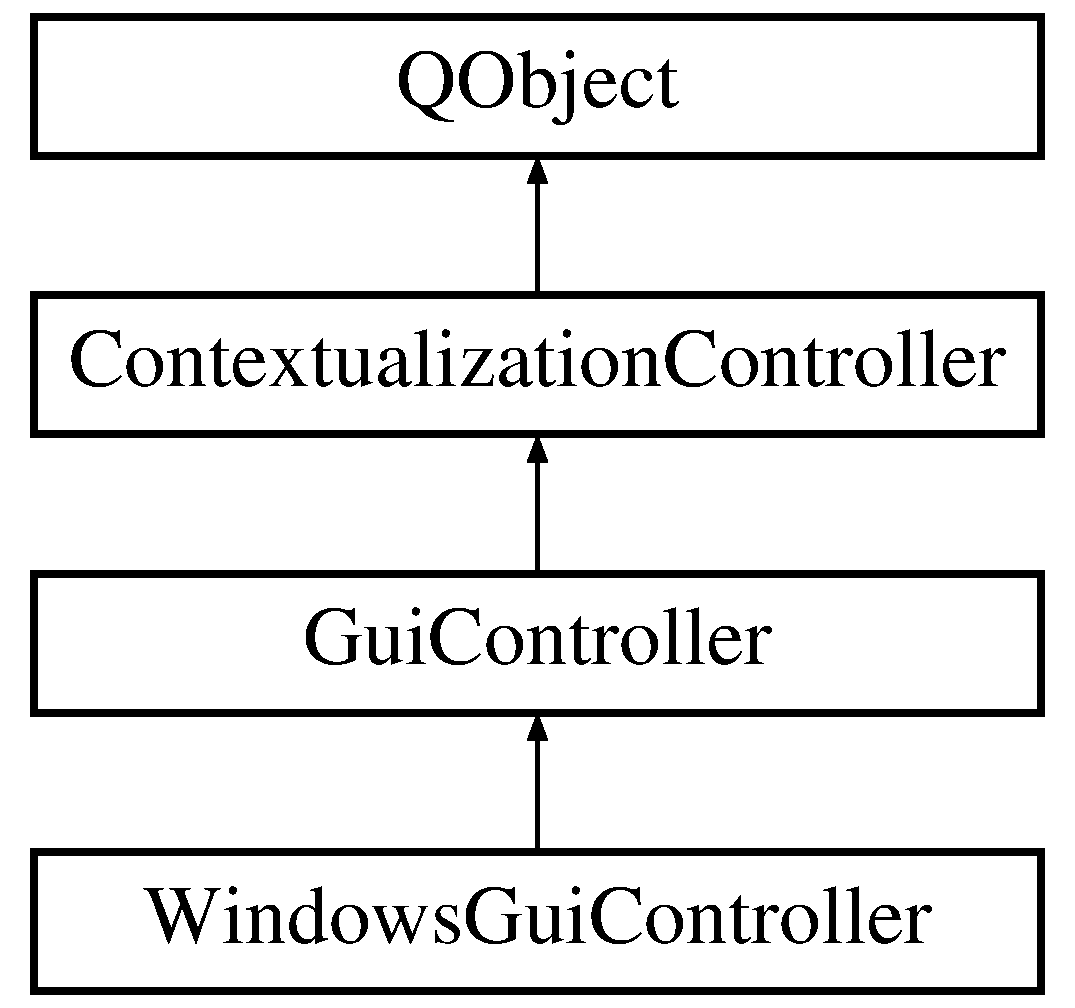
\includegraphics[height=4.000000cm]{classWindowsGuiController}
\end{center}
\end{figure}
\subsection*{Public Member Functions}
\begin{DoxyCompactItemize}
\item 
\mbox{\Hypertarget{classWindowsGuiController_ac6bbeedbefdf126c07e4b8a9b0f82d10}\label{classWindowsGuiController_ac6bbeedbefdf126c07e4b8a9b0f82d10}} 
{\bfseries Windows\+Gui\+Controller} (Q\+Quick\+Window $\ast$view=Q\+\_\+\+N\+U\+L\+L\+P\+TR, Q\+Object $\ast$parent=Q\+\_\+\+N\+U\+L\+L\+P\+TR)
\item 
Q\+String \mbox{\hyperlink{classWindowsGuiController_afcda369c002842873b3fb3cc3a593c06}{take\+Capture\+Area}} () override
\begin{DoxyCompactList}\small\item\em Starts a process that allow user capture an area of the screen. \end{DoxyCompactList}\item 
int \mbox{\hyperlink{classWindowsGuiController_aa78e32ce3635fc99f846d545d4a320b3}{generate\+Done\+Fp\+File}} () override
\begin{DoxyCompactList}\small\item\em Creates a copy of english\+Fp file in /tmp with only firmware strings with D\+O\+NE status. \end{DoxyCompactList}\end{DoxyCompactItemize}
\subsection*{Additional Inherited Members}


\subsection{Detailed Description}
This is the controller class that works a G\+UI Windows environment. 

Definition at line 20 of file windowsguicontroller.\+h.



\subsection{Member Function Documentation}
\mbox{\Hypertarget{classWindowsGuiController_aa78e32ce3635fc99f846d545d4a320b3}\label{classWindowsGuiController_aa78e32ce3635fc99f846d545d4a320b3}} 
\index{Windows\+Gui\+Controller@{Windows\+Gui\+Controller}!generate\+Done\+Fp\+File@{generate\+Done\+Fp\+File}}
\index{generate\+Done\+Fp\+File@{generate\+Done\+Fp\+File}!Windows\+Gui\+Controller@{Windows\+Gui\+Controller}}
\subsubsection{\texorpdfstring{generate\+Done\+Fp\+File()}{generateDoneFpFile()}}
{\footnotesize\ttfamily int Windows\+Gui\+Controller\+::generate\+Done\+Fp\+File (\begin{DoxyParamCaption}{ }\end{DoxyParamCaption})\hspace{0.3cm}{\ttfamily [override]}, {\ttfamily [virtual]}}



Creates a copy of english\+Fp file in /tmp with only firmware strings with D\+O\+NE status. 

If copy was created succesfully returns 0, otherwise returns the code error. \begin{DoxyReturn}{Returns}
Code error 
\end{DoxyReturn}


Reimplemented from \mbox{\hyperlink{classContextualizationController_af142a8bbd561278c3423ccad3b40c910}{Contextualization\+Controller}}.



Definition at line 29 of file windowsguicontroller.\+cpp.

\mbox{\Hypertarget{classWindowsGuiController_afcda369c002842873b3fb3cc3a593c06}\label{classWindowsGuiController_afcda369c002842873b3fb3cc3a593c06}} 
\index{Windows\+Gui\+Controller@{Windows\+Gui\+Controller}!take\+Capture\+Area@{take\+Capture\+Area}}
\index{take\+Capture\+Area@{take\+Capture\+Area}!Windows\+Gui\+Controller@{Windows\+Gui\+Controller}}
\subsubsection{\texorpdfstring{take\+Capture\+Area()}{takeCaptureArea()}}
{\footnotesize\ttfamily Q\+String Windows\+Gui\+Controller\+::take\+Capture\+Area (\begin{DoxyParamCaption}{ }\end{DoxyParamCaption})\hspace{0.3cm}{\ttfamily [override]}, {\ttfamily [virtual]}}



Starts a process that allow user capture an area of the screen. 

The user have to select the area to capture with the mouse. Return the path where the capture is stored or an empty Q\+String if an error ocurred. \begin{DoxyReturn}{Returns}
Q\+String 
\end{DoxyReturn}


Implements \mbox{\hyperlink{classContextualizationController_a121919886590cd4955bbcc2d8b747b26}{Contextualization\+Controller}}.



Definition at line 24 of file windowsguicontroller.\+cpp.



The documentation for this class was generated from the following files\+:\begin{DoxyCompactItemize}
\item 
src/contextualization/controller/\mbox{\hyperlink{windowsguicontroller_8h}{windowsguicontroller.\+h}}\item 
src/contextualization/controller/\mbox{\hyperlink{windowsguicontroller_8cpp}{windowsguicontroller.\+cpp}}\end{DoxyCompactItemize}

\chapter{File Documentation}
\hypertarget{consolecontroller_8cpp}{}\section{src/contextualization/controller/consolecontroller.cpp File Reference}
\label{consolecontroller_8cpp}\index{src/contextualization/controller/consolecontroller.\+cpp@{src/contextualization/controller/consolecontroller.\+cpp}}
{\ttfamily \#include \char`\"{}consolecontroller.\+h\char`\"{}}\newline


\subsection{Detailed Description}
\begin{DoxyAuthor}{Author}
Jorge Herrero Tardón (\href{mailto:jorgeht@usal.es}{\tt jorgeht@usal.\+es}) 
\end{DoxyAuthor}
\begin{DoxyDate}{Date}
20/02/2018 
\end{DoxyDate}
\begin{DoxyVersion}{Version}
1.\+0 
\end{DoxyVersion}

\hypertarget{consolecontroller_8h}{}\section{src/contextualization/controller/consolecontroller.h File Reference}
\label{consolecontroller_8h}\index{src/contextualization/controller/consolecontroller.\+h@{src/contextualization/controller/consolecontroller.\+h}}
{\ttfamily \#include $<$iostream$>$}\newline
{\ttfamily \#include $<$Q\+Variant$>$}\newline
{\ttfamily \#include $<$Q\+List$>$}\newline
{\ttfamily \#include $<$stdio.\+h$>$}\newline
{\ttfamily \#include $<$iomanip$>$}\newline
{\ttfamily \#include $<$string.\+h$>$}\newline
{\ttfamily \#include \char`\"{}contextualization/controller/contextualizationcontroller.\+h\char`\"{}}\newline
\subsection*{Classes}
\begin{DoxyCompactItemize}
\item 
class \mbox{\hyperlink{classConsoleController}{Console\+Controller}}
\begin{DoxyCompactList}\small\item\em The Console\+Contextualization\+Controller class is responsible for controll the Contextualization Tool application when is executed from a terminal (C\+LI). \end{DoxyCompactList}\end{DoxyCompactItemize}


\subsection{Detailed Description}
\begin{DoxyAuthor}{Author}
Jorge Herrero Tardón (\href{mailto:jorgeht@usal.es}{\tt jorgeht@usal.\+es}) 
\end{DoxyAuthor}
\begin{DoxyDate}{Date}
20/02/2018 
\end{DoxyDate}
\begin{DoxyVersion}{Version}
1.\+0 
\end{DoxyVersion}

\hypertarget{contextualizationcontroller_8cpp}{}\section{src/contextualization/controller/contextualizationcontroller.cpp File Reference}
\label{contextualizationcontroller_8cpp}\index{src/contextualization/controller/contextualizationcontroller.\+cpp@{src/contextualization/controller/contextualizationcontroller.\+cpp}}
{\ttfamily \#include \char`\"{}contextualizationcontroller.\+h\char`\"{}}\newline


\subsection{Detailed Description}
\begin{DoxyAuthor}{Author}
Jorge Herrero Tardón (\href{mailto:jorgeht@usal.es}{\tt jorgeht@usal.\+es}) 
\end{DoxyAuthor}
\begin{DoxyDate}{Date}
20/02/2018 
\end{DoxyDate}
\begin{DoxyVersion}{Version}
1.\+0 
\end{DoxyVersion}

\hypertarget{contextualizationcontroller_8h}{}\section{src/contextualization/controller/contextualizationcontroller.h File Reference}
\label{contextualizationcontroller_8h}\index{src/contextualization/controller/contextualizationcontroller.\+h@{src/contextualization/controller/contextualizationcontroller.\+h}}
{\ttfamily \#include $<$Q\+Object$>$}\newline
{\ttfamily \#include $<$Q\+String$>$}\newline
{\ttfamily \#include $<$Q\+String\+List$>$}\newline
{\ttfamily \#include $<$Q\+File$>$}\newline
{\ttfamily \#include $<$Q\+Standard\+Paths$>$}\newline
{\ttfamily \#include $<$Q\+Dir$>$}\newline
{\ttfamily \#include $<$Q\+Json\+Document$>$}\newline
{\ttfamily \#include $<$Q\+Json\+Object$>$}\newline
{\ttfamily \#include $<$Q\+Json\+Array$>$}\newline
{\ttfamily \#include $<$Q\+Regular\+Expression$>$}\newline
{\ttfamily \#include $<$Q\+Regular\+Expression\+Match$>$}\newline
{\ttfamily \#include $<$Q\+Image$>$}\newline
{\ttfamily \#include $<$Q\+Future$>$}\newline
{\ttfamily \#include $<$Qt\+Concurrent/\+Qt\+Concurrent$>$}\newline
{\ttfamily \#include \char`\"{}contextualization/model/contextualizationmodel.\+h\char`\"{}}\newline
{\ttfamily \#include \char`\"{}tools/utils.\+h\char`\"{}}\newline
{\ttfamily \#include \char`\"{}tools/log.\+h\char`\"{}}\newline
{\ttfamily \#include \char`\"{}optical\+\_\+character\+\_\+recognition/tesseractocr.\+h\char`\"{}}\newline
{\ttfamily \#include \char`\"{}storage/fpfileconnector.\+h\char`\"{}}\newline
{\ttfamily \#include \char`\"{}storage/mysqlconnector.\+h\char`\"{}}\newline
\subsection*{Classes}
\begin{DoxyCompactItemize}
\item 
class \mbox{\hyperlink{classContextualizationController}{Contextualization\+Controller}}
\begin{DoxyCompactList}\small\item\em This is the controller base class. \end{DoxyCompactList}\end{DoxyCompactItemize}


\subsection{Detailed Description}
\begin{DoxyAuthor}{Author}
Jorge Herrero Tardón (\href{mailto:jorgeht@usal.es}{\tt jorgeht@usal.\+es}) 
\end{DoxyAuthor}
\begin{DoxyDate}{Date}
20/02/2018 
\end{DoxyDate}
\begin{DoxyVersion}{Version}
1.\+0 
\end{DoxyVersion}

\hypertarget{guicontroller_8cpp}{}\section{src/contextualization/controller/guicontroller.cpp File Reference}
\label{guicontroller_8cpp}\index{src/contextualization/controller/guicontroller.\+cpp@{src/contextualization/controller/guicontroller.\+cpp}}
{\ttfamily \#include \char`\"{}guicontroller.\+h\char`\"{}}\newline


\subsection{Detailed Description}
\begin{DoxyAuthor}{Author}
Jorge Herrero Tardón (\href{mailto:jorgeht@usal.es}{\tt jorgeht@usal.\+es}) 
\end{DoxyAuthor}
\begin{DoxyDate}{Date}
20/02/2018 
\end{DoxyDate}
\begin{DoxyVersion}{Version}
1.\+0 
\end{DoxyVersion}

\hypertarget{guicontroller_8h}{}\section{src/contextualization/controller/guicontroller.h File Reference}
\label{guicontroller_8h}\index{src/contextualization/controller/guicontroller.\+h@{src/contextualization/controller/guicontroller.\+h}}
{\ttfamily \#include $<$Q\+Input\+Dialog$>$}\newline
{\ttfamily \#include $<$Q\+File\+Dialog$>$}\newline
{\ttfamily \#include $<$Q\+Application$>$}\newline
{\ttfamily \#include $<$Q\+Quick\+Window$>$}\newline
{\ttfamily \#include \char`\"{}contextualization/controller/contextualizationcontroller.\+h\char`\"{}}\newline
\subsection*{Classes}
\begin{DoxyCompactItemize}
\item 
class \mbox{\hyperlink{classGuiController}{Gui\+Controller}}
\begin{DoxyCompactList}\small\item\em This is the controller class that works a G\+UI environment. \end{DoxyCompactList}\end{DoxyCompactItemize}


\subsection{Detailed Description}
\begin{DoxyAuthor}{Author}
Jorge Herrero Tardón (\href{mailto:jorgeht@usal.es}{\tt jorgeht@usal.\+es}) 
\end{DoxyAuthor}
\begin{DoxyDate}{Date}
20/02/2018 
\end{DoxyDate}
\begin{DoxyVersion}{Version}
1.\+0 
\end{DoxyVersion}

\hypertarget{linuxconsolecontroller_8cpp}{}\section{src/contextualization/controller/linuxconsolecontroller.cpp File Reference}
\label{linuxconsolecontroller_8cpp}\index{src/contextualization/controller/linuxconsolecontroller.\+cpp@{src/contextualization/controller/linuxconsolecontroller.\+cpp}}
{\ttfamily \#include \char`\"{}linuxconsolecontroller.\+h\char`\"{}}\newline


\subsection{Detailed Description}
\begin{DoxyAuthor}{Author}
Jorge Herrero Tardón (\href{mailto:jorgeht@usal.es}{\tt jorgeht@usal.\+es}) 
\end{DoxyAuthor}
\begin{DoxyDate}{Date}
20/02/2018 
\end{DoxyDate}
\begin{DoxyVersion}{Version}
1.\+0 
\end{DoxyVersion}

\hypertarget{linuxconsolecontroller_8h}{}\section{src/contextualization/controller/linuxconsolecontroller.h File Reference}
\label{linuxconsolecontroller_8h}\index{src/contextualization/controller/linuxconsolecontroller.\+h@{src/contextualization/controller/linuxconsolecontroller.\+h}}
{\ttfamily \#include \char`\"{}consolecontroller.\+h\char`\"{}}\newline
\subsection*{Classes}
\begin{DoxyCompactItemize}
\item 
class \mbox{\hyperlink{classLinuxConsoleController}{Linux\+Console\+Controller}}
\begin{DoxyCompactList}\small\item\em This is the controller class that works a linux C\+LI environment. \end{DoxyCompactList}\end{DoxyCompactItemize}


\subsection{Detailed Description}
\begin{DoxyAuthor}{Author}
Jorge Herrero Tardón (\href{mailto:jorgeht@usal.es}{\tt jorgeht@usal.\+es}) 
\end{DoxyAuthor}
\begin{DoxyDate}{Date}
20/02/2018 
\end{DoxyDate}
\begin{DoxyVersion}{Version}
1.\+0 
\end{DoxyVersion}

\hypertarget{linuxguicontroller_8cpp}{}\section{src/contextualization/controller/linuxguicontroller.cpp File Reference}
\label{linuxguicontroller_8cpp}\index{src/contextualization/controller/linuxguicontroller.\+cpp@{src/contextualization/controller/linuxguicontroller.\+cpp}}
{\ttfamily \#include \char`\"{}linuxguicontroller.\+h\char`\"{}}\newline


\subsection{Detailed Description}
\begin{DoxyAuthor}{Author}
Jorge Herrero Tardón (\href{mailto:jorgeht@usal.es}{\tt jorgeht@usal.\+es}) 
\end{DoxyAuthor}
\begin{DoxyDate}{Date}
20/02/2018 
\end{DoxyDate}
\begin{DoxyVersion}{Version}
1.\+0 
\end{DoxyVersion}

\hypertarget{linuxguicontroller_8h}{}\section{src/contextualization/controller/linuxguicontroller.h File Reference}
\label{linuxguicontroller_8h}\index{src/contextualization/controller/linuxguicontroller.\+h@{src/contextualization/controller/linuxguicontroller.\+h}}
{\ttfamily \#include \char`\"{}guicontroller.\+h\char`\"{}}\newline
\subsection*{Classes}
\begin{DoxyCompactItemize}
\item 
class \mbox{\hyperlink{classLinuxGuiController}{Linux\+Gui\+Controller}}
\begin{DoxyCompactList}\small\item\em This is the controller class that works a linux G\+UI environment. \end{DoxyCompactList}\end{DoxyCompactItemize}


\subsection{Detailed Description}
\begin{DoxyAuthor}{Author}
Jorge Herrero Tardón (\href{mailto:jorgeht@usal.es}{\tt jorgeht@usal.\+es}) 
\end{DoxyAuthor}
\begin{DoxyDate}{Date}
20/02/2018 
\end{DoxyDate}
\begin{DoxyVersion}{Version}
1.\+0 
\end{DoxyVersion}

\hypertarget{windowsconsolecontroller_8cpp}{}\section{src/contextualization/controller/windowsconsolecontroller.cpp File Reference}
\label{windowsconsolecontroller_8cpp}\index{src/contextualization/controller/windowsconsolecontroller.\+cpp@{src/contextualization/controller/windowsconsolecontroller.\+cpp}}
{\ttfamily \#include \char`\"{}windowsconsolecontroller.\+h\char`\"{}}\newline


\subsection{Detailed Description}
\begin{DoxyAuthor}{Author}
Jorge Herrero Tardón (\href{mailto:jorgeht@usal.es}{\tt jorgeht@usal.\+es}) 
\end{DoxyAuthor}
\begin{DoxyDate}{Date}
20/02/2018 
\end{DoxyDate}
\begin{DoxyVersion}{Version}
1.\+0 
\end{DoxyVersion}

\hypertarget{windowsconsolecontroller_8h}{}\section{src/contextualization/controller/windowsconsolecontroller.h File Reference}
\label{windowsconsolecontroller_8h}\index{src/contextualization/controller/windowsconsolecontroller.\+h@{src/contextualization/controller/windowsconsolecontroller.\+h}}
{\ttfamily \#include \char`\"{}consolecontroller.\+h\char`\"{}}\newline
\subsection*{Classes}
\begin{DoxyCompactItemize}
\item 
class \mbox{\hyperlink{classWindowsConsoleController}{Windows\+Console\+Controller}}
\begin{DoxyCompactList}\small\item\em This is the controller class that works a Windows C\+LI environment. \end{DoxyCompactList}\end{DoxyCompactItemize}


\subsection{Detailed Description}
\begin{DoxyAuthor}{Author}
Jorge Herrero Tardón (\href{mailto:jorgeht@usal.es}{\tt jorgeht@usal.\+es}) 
\end{DoxyAuthor}
\begin{DoxyDate}{Date}
20/02/2018 
\end{DoxyDate}
\begin{DoxyVersion}{Version}
1.\+0 
\end{DoxyVersion}

\hypertarget{windowsguicontroller_8cpp}{}\section{src/contextualization/controller/windowsguicontroller.cpp File Reference}
\label{windowsguicontroller_8cpp}\index{src/contextualization/controller/windowsguicontroller.\+cpp@{src/contextualization/controller/windowsguicontroller.\+cpp}}
{\ttfamily \#include \char`\"{}windowsguicontroller.\+h\char`\"{}}\newline


\subsection{Detailed Description}
\begin{DoxyAuthor}{Author}
Jorge Herrero Tardón (\href{mailto:jorgeht@usal.es}{\tt jorgeht@usal.\+es}) 
\end{DoxyAuthor}
\begin{DoxyDate}{Date}
20/02/2018 
\end{DoxyDate}
\begin{DoxyVersion}{Version}
1.\+0 
\end{DoxyVersion}

\hypertarget{windowsguicontroller_8h}{}\section{src/contextualization/controller/windowsguicontroller.h File Reference}
\label{windowsguicontroller_8h}\index{src/contextualization/controller/windowsguicontroller.\+h@{src/contextualization/controller/windowsguicontroller.\+h}}
{\ttfamily \#include \char`\"{}guicontroller.\+h\char`\"{}}\newline
\subsection*{Classes}
\begin{DoxyCompactItemize}
\item 
class \mbox{\hyperlink{classWindowsGuiController}{Windows\+Gui\+Controller}}
\begin{DoxyCompactList}\small\item\em This is the controller class that works a G\+UI Windows environment. \end{DoxyCompactList}\end{DoxyCompactItemize}


\subsection{Detailed Description}
\begin{DoxyAuthor}{Author}
Jorge Herrero Tardón (\href{mailto:jorgeht@usal.es}{\tt jorgeht@usal.\+es}) 
\end{DoxyAuthor}
\begin{DoxyDate}{Date}
20/02/2018 
\end{DoxyDate}
\begin{DoxyVersion}{Version}
1.\+0 
\end{DoxyVersion}

\hypertarget{contextualizationmodel_8cpp}{}\section{src/contextualization/model/contextualizationmodel.cpp File Reference}
\label{contextualizationmodel_8cpp}\index{src/contextualization/model/contextualizationmodel.\+cpp@{src/contextualization/model/contextualizationmodel.\+cpp}}
{\ttfamily \#include \char`\"{}contextualizationmodel.\+h\char`\"{}}\newline


\subsection{Detailed Description}
\begin{DoxyAuthor}{Author}
Jorge Herrero Tardón (\href{mailto:jorgeht@usal.es}{\tt jorgeht@usal.\+es}) 
\end{DoxyAuthor}
\begin{DoxyDate}{Date}
20/02/2018 
\end{DoxyDate}
\begin{DoxyVersion}{Version}
1.\+0 
\end{DoxyVersion}

\hypertarget{contextualizationmodel_8h}{}\section{src/contextualization/model/contextualizationmodel.h File Reference}
\label{contextualizationmodel_8h}\index{src/contextualization/model/contextualizationmodel.\+h@{src/contextualization/model/contextualizationmodel.\+h}}
{\ttfamily \#include $<$Q\+Object$>$}\newline
{\ttfamily \#include $<$Q\+String$>$}\newline
{\ttfamily \#include $<$Q\+List$>$}\newline
{\ttfamily \#include $<$Q\+Dir$>$}\newline
{\ttfamily \#include $<$Q\+Json\+Document$>$}\newline
{\ttfamily \#include $<$Q\+Json\+Object$>$}\newline
{\ttfamily \#include \char`\"{}firmwarestring.\+h\char`\"{}}\newline
{\ttfamily \#include \char`\"{}src/tools/log.\+h\char`\"{}}\newline
\subsection*{Classes}
\begin{DoxyCompactItemize}
\item 
class \mbox{\hyperlink{classContextualizationModel}{Contextualization\+Model}}
\begin{DoxyCompactList}\small\item\em This is the model class of a M\+VC architecture on Contextualization Tool app. \end{DoxyCompactList}\end{DoxyCompactItemize}


\subsection{Detailed Description}
\begin{DoxyAuthor}{Author}
Jorge Herrero Tardón (\href{mailto:jorgeht@usal.es}{\tt jorgeht@usal.\+es}) 
\end{DoxyAuthor}
\begin{DoxyDate}{Date}
20/02/2018 
\end{DoxyDate}
\begin{DoxyVersion}{Version}
1.\+0 
\end{DoxyVersion}

\hypertarget{firmwarestring_8cpp}{}\section{src/contextualization/model/firmwarestring.cpp File Reference}
\label{firmwarestring_8cpp}\index{src/contextualization/model/firmwarestring.\+cpp@{src/contextualization/model/firmwarestring.\+cpp}}
{\ttfamily \#include \char`\"{}firmwarestring.\+h\char`\"{}}\newline


\subsection{Detailed Description}
\begin{DoxyAuthor}{Author}
Jorge Herrero Tardón (\href{mailto:jorgeht@usal.es}{\tt jorgeht@usal.\+es}) 
\end{DoxyAuthor}
\begin{DoxyDate}{Date}
20/02/2018 
\end{DoxyDate}
\begin{DoxyVersion}{Version}
1.\+0 
\end{DoxyVersion}

\hypertarget{firmwarestring_8h}{}\section{src/contextualization/model/firmwarestring.h File Reference}
\label{firmwarestring_8h}\index{src/contextualization/model/firmwarestring.\+h@{src/contextualization/model/firmwarestring.\+h}}
{\ttfamily \#include \char`\"{}string.\+h\char`\"{}}\newline
\subsection*{Classes}
\begin{DoxyCompactItemize}
\item 
class \mbox{\hyperlink{classFirmwareString}{Firmware\+String}}
\begin{DoxyCompactList}\small\item\em This a representation of a Firmware \mbox{\hyperlink{classString}{String}} used in HP company. \end{DoxyCompactList}\end{DoxyCompactItemize}


\subsection{Detailed Description}
\begin{DoxyAuthor}{Author}
Jorge Herrero Tardón (\href{mailto:jorgeht@usal.es}{\tt jorgeht@usal.\+es}) 
\end{DoxyAuthor}
\begin{DoxyDate}{Date}
20/02/2018 
\end{DoxyDate}
\begin{DoxyVersion}{Version}
1.\+0 
\end{DoxyVersion}

\hypertarget{string_8cpp}{}\section{src/contextualization/model/string.cpp File Reference}
\label{string_8cpp}\index{src/contextualization/model/string.\+cpp@{src/contextualization/model/string.\+cpp}}
{\ttfamily \#include \char`\"{}string.\+h\char`\"{}}\newline


\subsection{Detailed Description}
\begin{DoxyAuthor}{Author}
Jorge Herrero Tardón (\href{mailto:jorgeht@usal.es}{\tt jorgeht@usal.\+es}) 
\end{DoxyAuthor}
\begin{DoxyDate}{Date}
20/02/2018 
\end{DoxyDate}
\begin{DoxyVersion}{Version}
1.\+0 
\end{DoxyVersion}

\hypertarget{string_8h}{}\section{src/contextualization/model/string.h File Reference}
\label{string_8h}\index{src/contextualization/model/string.\+h@{src/contextualization/model/string.\+h}}
{\ttfamily \#include $<$Q\+String$>$}\newline
{\ttfamily \#include $<$Q\+Json\+Document$>$}\newline
{\ttfamily \#include $<$Q\+Json\+Object$>$}\newline
{\ttfamily \#include $<$Q\+Regular\+Expression$>$}\newline
{\ttfamily \#include \char`\"{}tools/log.\+h\char`\"{}}\newline
\subsection*{Classes}
\begin{DoxyCompactItemize}
\item 
class \mbox{\hyperlink{classString}{String}}
\begin{DoxyCompactList}\small\item\em This is the representation of a string with their properties. \end{DoxyCompactList}\end{DoxyCompactItemize}


\subsection{Detailed Description}
\begin{DoxyAuthor}{Author}
Jorge Herrero Tardón (\href{mailto:jorgeht@usal.es}{\tt jorgeht@usal.\+es}) 
\end{DoxyAuthor}
\begin{DoxyDate}{Date}
20/02/2018 
\end{DoxyDate}
\begin{DoxyVersion}{Version}
1.\+0 
\end{DoxyVersion}

\hypertarget{main_8cpp}{}\section{src/main.cpp File Reference}
\label{main_8cpp}\index{src/main.\+cpp@{src/main.\+cpp}}


This main file to exec program.  


{\ttfamily \#include $<$Q\+Application$>$}\newline
{\ttfamily \#include $<$Q\+Qml\+Application\+Engine$>$}\newline
{\ttfamily \#include $<$Q\+Qml\+Context$>$}\newline
{\ttfamily \#include \char`\"{}tools/hpcontextualizationfactory.\+h\char`\"{}}\newline
{\ttfamily \#include $<$Q\+Debug$>$}\newline
\subsection*{Functions}
\begin{DoxyCompactItemize}
\item 
int \mbox{\hyperlink{main_8cpp_a0ddf1224851353fc92bfbff6f499fa97}{main}} (int argc, char $\ast$argv\mbox{[}$\,$\mbox{]})
\end{DoxyCompactItemize}


\subsection{Detailed Description}
This main file to exec program. 

\begin{DoxyAuthor}{Author}
Jorge Herrero Tardón (\href{mailto:jorgeht@usal.es}{\tt jorgeht@usal.\+es}) 
\end{DoxyAuthor}
\begin{DoxyDate}{Date}
20/02/2018 
\end{DoxyDate}
\begin{DoxyVersion}{Version}
1.\+0 
\end{DoxyVersion}


\subsection{Function Documentation}
\mbox{\Hypertarget{main_8cpp_a0ddf1224851353fc92bfbff6f499fa97}\label{main_8cpp_a0ddf1224851353fc92bfbff6f499fa97}} 
\index{main.\+cpp@{main.\+cpp}!main@{main}}
\index{main@{main}!main.\+cpp@{main.\+cpp}}
\subsubsection{\texorpdfstring{main()}{main()}}
{\footnotesize\ttfamily int main (\begin{DoxyParamCaption}\item[{int}]{argc,  }\item[{char $\ast$}]{argv\mbox{[}$\,$\mbox{]} }\end{DoxyParamCaption})}

The Gui\+Contextualization\+Controller class is registered as a type, which is accessible from Q\+ML by importing the U\+RL, \char`\"{}io.\+controllers.\+guicontroller 1.\+0\char`\"{}.

Definition at line 16 of file main.\+cpp.


\hypertarget{ocr_8cpp}{}\section{src/optical\+\_\+character\+\_\+recognition/ocr.cpp File Reference}
\label{ocr_8cpp}\index{src/optical\+\_\+character\+\_\+recognition/ocr.\+cpp@{src/optical\+\_\+character\+\_\+recognition/ocr.\+cpp}}
{\ttfamily \#include \char`\"{}ocr.\+h\char`\"{}}\newline


\subsection{Detailed Description}
\begin{DoxyAuthor}{Author}
Jorge Herrero Tardón (\href{mailto:jorgeht@usal.es}{\tt jorgeht@usal.\+es}) 
\end{DoxyAuthor}
\begin{DoxyDate}{Date}
20/02/2018 
\end{DoxyDate}
\begin{DoxyVersion}{Version}
1.\+0 
\end{DoxyVersion}

\hypertarget{ocr_8h}{}\section{src/optical\+\_\+character\+\_\+recognition/ocr.h File Reference}
\label{ocr_8h}\index{src/optical\+\_\+character\+\_\+recognition/ocr.\+h@{src/optical\+\_\+character\+\_\+recognition/ocr.\+h}}
{\ttfamily \#include $<$Q\+String$>$}\newline
{\ttfamily \#include $<$Q\+String\+List$>$}\newline
{\ttfamily \#include $<$Q\+Dir$>$}\newline
{\ttfamily \#include $<$Q\+File$>$}\newline
{\ttfamily \#include $<$Q\+File\+Info$>$}\newline
{\ttfamily \#include $<$Q\+Image$>$}\newline
{\ttfamily \#include $<$Q\+Regular\+Expression$>$}\newline
{\ttfamily \#include \char`\"{}tools/log.\+h\char`\"{}}\newline
\subsection*{Classes}
\begin{DoxyCompactItemize}
\item 
class \mbox{\hyperlink{classOcr}{Ocr}}
\begin{DoxyCompactList}\small\item\em This is an interface for a optical character recognition api. \end{DoxyCompactList}\end{DoxyCompactItemize}


\subsection{Detailed Description}
\begin{DoxyAuthor}{Author}
Jorge Herrero Tardón (\href{mailto:jorgeht@usal.es}{\tt jorgeht@usal.\+es}) 
\end{DoxyAuthor}
\begin{DoxyDate}{Date}
20/02/2018 
\end{DoxyDate}
\begin{DoxyVersion}{Version}
1.\+0 
\end{DoxyVersion}

\hypertarget{tesseractocr_8cpp}{}\section{src/optical\+\_\+character\+\_\+recognition/tesseractocr.cpp File Reference}
\label{tesseractocr_8cpp}\index{src/optical\+\_\+character\+\_\+recognition/tesseractocr.\+cpp@{src/optical\+\_\+character\+\_\+recognition/tesseractocr.\+cpp}}
{\ttfamily \#include \char`\"{}tesseractocr.\+h\char`\"{}}\newline


\subsection{Detailed Description}
\begin{DoxyAuthor}{Author}
Jorge Herrero Tardón (\href{mailto:jorgeht@usal.es}{\tt jorgeht@usal.\+es}) 
\end{DoxyAuthor}
\begin{DoxyDate}{Date}
20/02/2018 
\end{DoxyDate}
\begin{DoxyVersion}{Version}
1.\+0 
\end{DoxyVersion}

\hypertarget{tesseractocr_8h}{}\section{src/optical\+\_\+character\+\_\+recognition/tesseractocr.h File Reference}
\label{tesseractocr_8h}\index{src/optical\+\_\+character\+\_\+recognition/tesseractocr.\+h@{src/optical\+\_\+character\+\_\+recognition/tesseractocr.\+h}}
{\ttfamily \#include $<$leptonica/allheaders.\+h$>$}\newline
{\ttfamily \#include \char`\"{}baseapi.\+h\char`\"{}}\newline
{\ttfamily \#include \char`\"{}genericvector.\+h\char`\"{}}\newline
{\ttfamily \#include \char`\"{}ocr.\+h\char`\"{}}\newline
{\ttfamily \#include \char`\"{}tools/utils.\+h\char`\"{}}\newline
{\ttfamily \#include \char`\"{}tools/log.\+h\char`\"{}}\newline
\subsection*{Classes}
\begin{DoxyCompactItemize}
\item 
class \mbox{\hyperlink{classTesseractOcr}{Tesseract\+Ocr}}
\begin{DoxyCompactList}\small\item\em This is a tool to detect string on images using tesseract api (\href{https://github.com/tesseract-ocr/tesseract}{\tt https\+://github.\+com/tesseract-\/ocr/tesseract}). \end{DoxyCompactList}\end{DoxyCompactItemize}


\subsection{Detailed Description}
\begin{DoxyAuthor}{Author}
Jorge Herrero Tardón (\href{mailto:jorgeht@usal.es}{\tt jorgeht@usal.\+es}) 
\end{DoxyAuthor}
\begin{DoxyDate}{Date}
20/02/2018 
\end{DoxyDate}
\begin{DoxyVersion}{Version}
1.\+0 
\end{DoxyVersion}

\hypertarget{databaseconnectorabstract_8cpp}{}\section{src/storage/databaseconnectorabstract.cpp File Reference}
\label{databaseconnectorabstract_8cpp}\index{src/storage/databaseconnectorabstract.\+cpp@{src/storage/databaseconnectorabstract.\+cpp}}
{\ttfamily \#include \char`\"{}databaseconnectorabstract.\+h\char`\"{}}\newline


\subsection{Detailed Description}
\begin{DoxyAuthor}{Author}
Jorge Herrero Tardón (\href{mailto:jorgeht@usal.es}{\tt jorgeht@usal.\+es}) 
\end{DoxyAuthor}
\begin{DoxyDate}{Date}
20/02/2018 
\end{DoxyDate}
\begin{DoxyVersion}{Version}
1.\+0 
\end{DoxyVersion}

\hypertarget{databaseconnectorabstract_8h}{}\section{src/storage/databaseconnectorabstract.h File Reference}
\label{databaseconnectorabstract_8h}\index{src/storage/databaseconnectorabstract.\+h@{src/storage/databaseconnectorabstract.\+h}}
{\ttfamily \#include \char`\"{}contextualization/model/string.\+h\char`\"{}}\newline
{\ttfamily \#include \char`\"{}tools/log.\+h\char`\"{}}\newline
{\ttfamily \#include \char`\"{}tools/utils.\+h\char`\"{}}\newline
\subsection*{Classes}
\begin{DoxyCompactItemize}
\item 
class \mbox{\hyperlink{classDatabaseConnectorAbstract}{Database\+Connector\+Abstract}}
\begin{DoxyCompactList}\small\item\em This is an interface to access a different data bases. \end{DoxyCompactList}\end{DoxyCompactItemize}


\subsection{Detailed Description}
\begin{DoxyAuthor}{Author}
Jorge Herrero Tardón (\href{mailto:jorgeht@usal.es}{\tt jorgeht@usal.\+es}) 
\end{DoxyAuthor}
\begin{DoxyDate}{Date}
20/02/2018 
\end{DoxyDate}
\begin{DoxyVersion}{Version}
1.\+0 
\end{DoxyVersion}

\hypertarget{fpfileconnector_8h}{}\section{src/storage/fpfileconnector.h File Reference}
\label{fpfileconnector_8h}\index{src/storage/fpfileconnector.\+h@{src/storage/fpfileconnector.\+h}}
{\ttfamily \#include $<$Q\+File$>$}\newline
{\ttfamily \#include $<$Q\+File\+Info$>$}\newline
{\ttfamily \#include $<$Q\+Dir$>$}\newline
{\ttfamily \#include \char`\"{}databaseconnectorabstract.\+h\char`\"{}}\newline
{\ttfamily \#include \char`\"{}contextualization/model/firmwarestring.\+h\char`\"{}}\newline
{\ttfamily \#include \char`\"{}tools/utils.\+h\char`\"{}}\newline
\subsection*{Classes}
\begin{DoxyCompactItemize}
\item 
class \mbox{\hyperlink{classFpFileConnector}{Fp\+File\+Connector}}
\begin{DoxyCompactList}\small\item\em This is a class to access a database saved as fp file by HP company. \end{DoxyCompactList}\end{DoxyCompactItemize}


\subsection{Detailed Description}
\begin{DoxyAuthor}{Author}
Jorge Herrero Tardón (\href{mailto:jorgeht@usal.es}{\tt jorgeht@usal.\+es}) 
\end{DoxyAuthor}
\begin{DoxyDate}{Date}
20/02/2018 
\end{DoxyDate}
\begin{DoxyVersion}{Version}
1.\+0 
\end{DoxyVersion}

\hypertarget{mysqlconnector_8cpp}{}\section{src/storage/mysqlconnector.cpp File Reference}
\label{mysqlconnector_8cpp}\index{src/storage/mysqlconnector.\+cpp@{src/storage/mysqlconnector.\+cpp}}
{\ttfamily \#include \char`\"{}mysqlconnector.\+h\char`\"{}}\newline


\subsection{Detailed Description}
\begin{DoxyAuthor}{Author}
Jorge Herrero Tardón (\href{mailto:jorgeht@usal.es}{\tt jorgeht@usal.\+es}) 
\end{DoxyAuthor}
\begin{DoxyDate}{Date}
20/02/2018 
\end{DoxyDate}
\begin{DoxyVersion}{Version}
1.\+0 
\end{DoxyVersion}

\hypertarget{mysqlconnector_8h}{}\section{src/storage/mysqlconnector.h File Reference}
\label{mysqlconnector_8h}\index{src/storage/mysqlconnector.\+h@{src/storage/mysqlconnector.\+h}}
{\ttfamily \#include $<$Qt\+Sql/\+Q\+Sql\+Database$>$}\newline
{\ttfamily \#include $<$Qt\+Sql/\+Q\+Sql\+Query$>$}\newline
{\ttfamily \#include $<$Qt\+Sql/\+Q\+Sql\+Error$>$}\newline
{\ttfamily \#include \char`\"{}contextualization/model/firmwarestring.\+h\char`\"{}}\newline
{\ttfamily \#include \char`\"{}databaseconnectorabstract.\+h\char`\"{}}\newline
\subsection*{Classes}
\begin{DoxyCompactItemize}
\item 
class \mbox{\hyperlink{classMySqlConnector}{My\+Sql\+Connector}}
\begin{DoxyCompactList}\small\item\em This is a class to access a My\+S\+QL database. \end{DoxyCompactList}\end{DoxyCompactItemize}


\subsection{Detailed Description}
\begin{DoxyAuthor}{Author}
Jorge Herrero Tardón (\href{mailto:jorgeht@usal.es}{\tt jorgeht@usal.\+es}) 
\end{DoxyAuthor}
\begin{DoxyDate}{Date}
20/02/2018 
\end{DoxyDate}
\begin{DoxyVersion}{Version}
1.\+0 
\end{DoxyVersion}

\hypertarget{contextualizationfactoryabstract_8cpp}{}\section{src/tools/contextualizationfactoryabstract.cpp File Reference}
\label{contextualizationfactoryabstract_8cpp}\index{src/tools/contextualizationfactoryabstract.\+cpp@{src/tools/contextualizationfactoryabstract.\+cpp}}
{\ttfamily \#include \char`\"{}contextualizationfactoryabstract.\+h\char`\"{}}\newline


\subsection{Detailed Description}
\begin{DoxyAuthor}{Author}
Jorge Herrero Tardón (\href{mailto:jorgeht@usal.es}{\tt jorgeht@usal.\+es}) 
\end{DoxyAuthor}
\begin{DoxyDate}{Date}
20/02/2018 
\end{DoxyDate}
\begin{DoxyVersion}{Version}
1.\+0 
\end{DoxyVersion}

\hypertarget{contextualizationfactoryabstract_8h}{}\section{src/tools/contextualizationfactoryabstract.h File Reference}
\label{contextualizationfactoryabstract_8h}\index{src/tools/contextualizationfactoryabstract.\+h@{src/tools/contextualizationfactoryabstract.\+h}}
{\ttfamily \#include $<$Q\+Sys\+Info$>$}\newline
{\ttfamily \#include \char`\"{}contextualization/controller/contextualizationcontroller.\+h\char`\"{}}\newline
\subsection*{Classes}
\begin{DoxyCompactItemize}
\item 
class \mbox{\hyperlink{classContextualizationFactoryAbstract}{Contextualization\+Factory\+Abstract}}
\begin{DoxyCompactList}\small\item\em This is a interface factory to create a concrete class of \mbox{\hyperlink{classContextualizationController}{Contextualization\+Controller}}. \end{DoxyCompactList}\end{DoxyCompactItemize}


\subsection{Detailed Description}
\begin{DoxyAuthor}{Author}
Jorge Herrero Tardón (\href{mailto:jorgeht@usal.es}{\tt jorgeht@usal.\+es}) 
\end{DoxyAuthor}
\begin{DoxyDate}{Date}
20/02/2018 
\end{DoxyDate}
\begin{DoxyVersion}{Version}
1.\+0 
\end{DoxyVersion}

\hypertarget{hpcontextualizationfactory_8cpp}{}\section{src/tools/hpcontextualizationfactory.cpp File Reference}
\label{hpcontextualizationfactory_8cpp}\index{src/tools/hpcontextualizationfactory.\+cpp@{src/tools/hpcontextualizationfactory.\+cpp}}
{\ttfamily \#include \char`\"{}hpcontextualizationfactory.\+h\char`\"{}}\newline


\subsection{Detailed Description}
\begin{DoxyAuthor}{Author}
Jorge Herrero Tardón (\href{mailto:jorgeht@usal.es}{\tt jorgeht@usal.\+es}) 
\end{DoxyAuthor}
\begin{DoxyDate}{Date}
20/02/2018 
\end{DoxyDate}
\begin{DoxyVersion}{Version}
1.\+0 
\end{DoxyVersion}

\hypertarget{hpcontextualizationfactory_8h}{}\section{src/tools/hpcontextualizationfactory.h File Reference}
\label{hpcontextualizationfactory_8h}\index{src/tools/hpcontextualizationfactory.\+h@{src/tools/hpcontextualizationfactory.\+h}}
{\ttfamily \#include \char`\"{}contextualizationfactoryabstract.\+h\char`\"{}}\newline
{\ttfamily \#include \char`\"{}contextualization/controller/linuxconsolecontroller.\+h\char`\"{}}\newline
{\ttfamily \#include \char`\"{}contextualization/controller/linuxguicontroller.\+h\char`\"{}}\newline
{\ttfamily \#include \char`\"{}contextualization/controller/windowsconsolecontroller.\+h\char`\"{}}\newline
{\ttfamily \#include \char`\"{}contextualization/controller/windowsguicontroller.\+h\char`\"{}}\newline
{\ttfamily \#include \char`\"{}tools/utils.\+h\char`\"{}}\newline
\subsection*{Classes}
\begin{DoxyCompactItemize}
\item 
class \mbox{\hyperlink{classHpContextualizationFactory}{Hp\+Contextualization\+Factory}}
\begin{DoxyCompactList}\small\item\em This is a factory to create a concrete class of \mbox{\hyperlink{classContextualizationController}{Contextualization\+Controller}} specific for HP company. \end{DoxyCompactList}\end{DoxyCompactItemize}


\subsection{Detailed Description}
\begin{DoxyAuthor}{Author}
Jorge Herrero Tardón (\href{mailto:jorgeht@usal.es}{\tt jorgeht@usal.\+es}) 
\end{DoxyAuthor}
\begin{DoxyDate}{Date}
20/02/2018 
\end{DoxyDate}
\begin{DoxyVersion}{Version}
1.\+0 
\end{DoxyVersion}

\hypertarget{log_8cpp}{}\section{src/tools/log.cpp File Reference}
\label{log_8cpp}\index{src/tools/log.\+cpp@{src/tools/log.\+cpp}}
{\ttfamily \#include \char`\"{}log.\+h\char`\"{}}\newline


\subsection{Detailed Description}
\begin{DoxyAuthor}{Author}
Jorge Herrero Tardón (\href{mailto:jorgeht@usal.es}{\tt jorgeht@usal.\+es}) 
\end{DoxyAuthor}
\begin{DoxyDate}{Date}
20/02/2018 
\end{DoxyDate}
\begin{DoxyVersion}{Version}
1.\+0 
\end{DoxyVersion}

\hypertarget{log_8h}{}\section{src/tools/log.h File Reference}
\label{log_8h}\index{src/tools/log.\+h@{src/tools/log.\+h}}
{\ttfamily \#include $<$Q\+String$>$}\newline
{\ttfamily \#include $<$Q\+File$>$}\newline
{\ttfamily \#include $<$Q\+Text\+Stream$>$}\newline
{\ttfamily \#include $<$Q\+Date$>$}\newline
{\ttfamily \#include $<$Q\+Standard\+Paths$>$}\newline
{\ttfamily \#include $<$Q\+Debug$>$}\newline
\subsection*{Classes}
\begin{DoxyCompactItemize}
\item 
class \mbox{\hyperlink{classLog}{Log}}
\begin{DoxyCompactList}\small\item\em This is a static class to write logs in different channels. \end{DoxyCompactList}\end{DoxyCompactItemize}


\subsection{Detailed Description}
\begin{DoxyAuthor}{Author}
Jorge Herrero Tardón (\href{mailto:jorgeht@usal.es}{\tt jorgeht@usal.\+es}) 
\end{DoxyAuthor}
\begin{DoxyDate}{Date}
20/02/2018 
\end{DoxyDate}
\begin{DoxyVersion}{Version}
1.\+0 
\end{DoxyVersion}

\hypertarget{utils_8cpp}{}\section{src/tools/utils.cpp File Reference}
\label{utils_8cpp}\index{src/tools/utils.\+cpp@{src/tools/utils.\+cpp}}
{\ttfamily \#include \char`\"{}utils.\+h\char`\"{}}\newline


\subsection{Detailed Description}
\begin{DoxyAuthor}{Author}
Jorge Herrero Tardón (\href{mailto:jorgeht@usal.es}{\tt jorgeht@usal.\+es}) 
\end{DoxyAuthor}
\begin{DoxyDate}{Date}
20/02/2018 
\end{DoxyDate}
\begin{DoxyVersion}{Version}
1.\+0 
\end{DoxyVersion}

\hypertarget{utils_8h}{}\section{src/tools/utils.h File Reference}
\label{utils_8h}\index{src/tools/utils.\+h@{src/tools/utils.\+h}}
{\ttfamily \#include $<$Q\+Dir$>$}\newline
{\ttfamily \#include $<$Q\+File$>$}\newline
{\ttfamily \#include $<$Q\+Message\+Box$>$}\newline
{\ttfamily \#include $<$Q\+Process$>$}\newline
{\ttfamily \#include $<$Q\+Progress\+Dialog$>$}\newline
{\ttfamily \#include $<$Q\+String$>$}\newline
{\ttfamily \#include $<$Q\+Thread$>$}\newline
{\ttfamily \#include $<$Q\+Future$>$}\newline
{\ttfamily \#include $<$Qt\+Concurrent/\+Qt\+Concurrent$>$}\newline
{\ttfamily \#include $<$Q\+Date\+Time$>$}\newline
\subsection*{Classes}
\begin{DoxyCompactItemize}
\item 
class \mbox{\hyperlink{classUtils}{Utils}}
\begin{DoxyCompactList}\small\item\em This is static class with a lot of different utilities. \end{DoxyCompactList}\end{DoxyCompactItemize}


\subsection{Detailed Description}
\begin{DoxyAuthor}{Author}
Jorge Herrero Tardón (\href{mailto:jorgeht@usal.es}{\tt jorgeht@usal.\+es}) 
\end{DoxyAuthor}
\begin{DoxyDate}{Date}
20/02/2018 
\end{DoxyDate}
\begin{DoxyVersion}{Version}
1.\+0 
\end{DoxyVersion}

%--- End generated contents ---

% Index
\backmatter
\newpage
\phantomsection
\clearemptydoublepage
\addcontentsline{toc}{chapter}{\indexname}
\printindex

\end{document}
